\documentclass[12pt,a4paper]{jarticle}

\usepackage{graphicx}
\usepackage{fancyhdr}
\usepackage{lastpage}
\usepackage{fancyhdr}
\usepackage{ascmac}
\usepackage[dvipdfmx]{graphicx}
\usepackage{here}
\usepackage{float}
\usepackage{framed}
\usepackage{array}
\usepackage[top=30truemm,bottom=30truemm,left=25truemm,right=25truemm]{geometry}
\pagestyle{fancy}
\lhead{\scriptsize Webプログラミング \quad -レポート課題 (第9回)-}
\rhead{\scriptsize 学籍番号:201711466 \quad 氏名:平井李音}
\cfoot{\thepage{}/{}\pageref{LastPage}}
\renewcommand{\thesection}{(\arabic{section})}
\renewcommand{\thesubsection}{\arabic{subsection}}

\begin{document}
\begin{ttfamily}

\section{アプリケーションの概要、特徴、工夫した点等の解説}
\subsection{概要}
このアプリケーションは、小説や漫画といった物語を作る上で、その世界特有の用語や登場キャラクターについてまとめるためのものです。
\subsection{特徴}
似たようなものとして@Wikiなどがあるが、それよりも簡単に編集が行える。
\subsection{工夫した点}
\subsubsection{パスワード}
作った世界、用語、キャラクターに任意でパスワードを設けることが出来る。
\par 世界にパスワードを設けることで、パスワードを知っている人だけに限定公開することが出来る。
\par 用語やキャラクターにパスワードを設けることで、勝手に内容を編集されることを防ぐことが出来る。
\subsubsection{セッション管理}
どのプログラムでも共通して使用する、作った世界に割り当てた「id」と「name」セッションで管理して一々HTML側で受け渡さなくて済むようにしている。
\subsubsection{同名項目作成の制限}
同名の世界、用語、キャラクターが作れないようにしてある。
\subsubsection{入力制限}
HTMLで表示しているため、HTMLのタグを入力されると困るため、語尾が「\_create2」になっているプログラム内で正規表現で「<.*>」を含む内容の入力を受け付けないようにしてある。
\subsubsection{改行}
正規表現によって、改行文字を「\verb|\|n」から「</br>」に置き換えることで、改行が行えるようにした。

\newpage
\section{ファイル間の関連、データ形式、プログラム等の解説}
\subsection{ファイル間の関連}
 \ \\
\begin{figure}[h]
  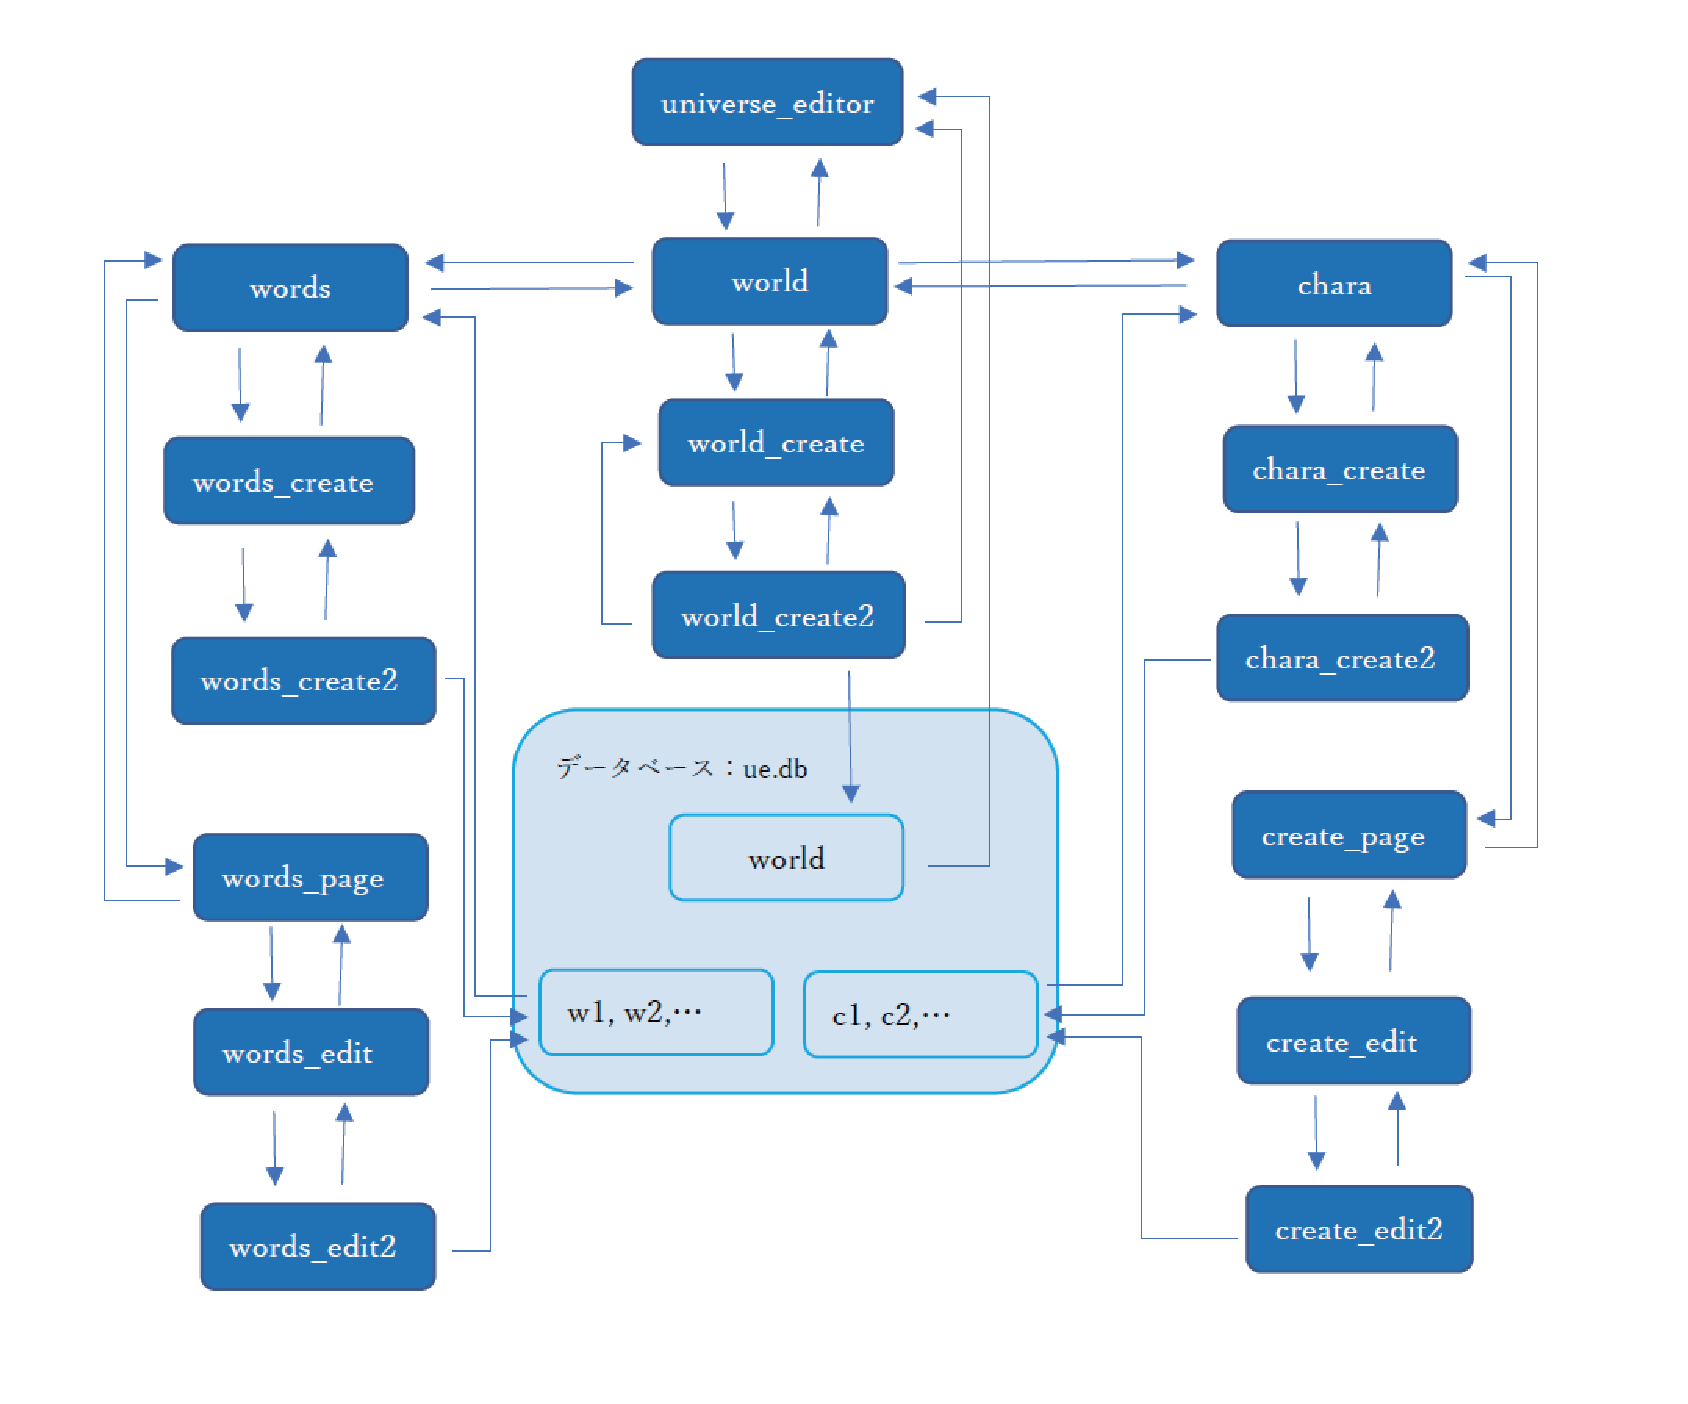
\includegraphics[width = 180mm]{10-2.eps}
  \centering
  \caption{ファイル間の関連}
\end{figure}
 \ \\
\subsection{データ形式}
使用しているデータは全てue.db形式で保存している。
\par テーブルは、「world」「w1, w2, ...」「c1, c2, ...」の3種類存在する。
\par worldテーブルの構成は、\\
 \ \ \ CREATE TABLE world (\\
 \ \ \ \ \ id INTEGER PRIMARY KEY,\\
 \ \ \ \ \ name TEXT NOT NULL,\\
 \ \ \ \ \ creator TEXT NOT NULL,\\
 \ \ \ \ \ summary TEXT NOT NULL,\\
 \ \ \ \ \ pass TEXT\\
 \ \ \ );\\
となっている。
\par w○テーブルの構成は、\\
 \ \ \ CREATE TABLE w○ (\\
 \ \ \ \ \ wid INTEGER PRIMARY KEY,\\
 \ \ \ \ \ creator TEXT NOT NULL,\\
 \ \ \ \ \ word TEXT NOT NULL,\\
 \ \ \ \ \ ruby TEXT NOT NULL,\\
 \ \ \ \ \ content TEXT NOT NULL,\\
 \ \ \ \ \ relation TEXT,\\
 \ \ \ \ \ pass TEXT\\
 \ \ \ );\\
となっている。
\par c○テーブルの構成は、\\
 \ \ \ CREATE TABLE c○ (\\
 \ \ \ \ \ cid INTEGER PRIMARY KEY,\\
 \ \ \ \ \ creator TEXT NOT NULL,\\
 \ \ \ \ \ chara TEXT NOT NULL,\\
 \ \ \ \ \ ruby TEXT NOT NULL,\\
 \ \ \ \ \ age INTEGER NOT NULL,\\
 \ \ \ \ \ sex TEXT NOT NULL,\\
 \ \ \ \ \ height INTEGER NOT NULL,\\
 \ \ \ \ \ weight INTEGER NOT NULL,\\
 \ \ \ \ \ content TEXT NOT NULL,\\
 \ \ \ \ \ relation TEXT,\\
 \ \ \ \ \ pass TEXT\\
 \ \ \ );\\
となっている。
\subsection{プログラムの解説}
このアプリケーションは基本的に、ホーム部分(universe\_editor, words, chara など)→○○\_create(もしくは○○\_edit)→ ○○\_create2(もしくは○○\_edit2)によって成立している。
\par ホーム部分がデータベースから該当するテーブルからデータを取得し、箇条書き形式表示する。また、これをリンク化してクリックすることで、詳細ページ(words\_page、chara\_page)に移動し、詳細な内容を見ることが出来る。
\par ○○\_createは単なる入力ホームであり、入力された内容を対応する○○\_create2に渡す。
\par ○○\_create2は○○\_createから渡されたデータをデータベースに追加・編集する役割を持つ。追加・編集する過程で正規表現により、HTMLのタグが入力されることを防いだり、改行文字を置き換えることでHTML上で改行されて表示されたりする機能を持つ。
\par なお、ソースコードはレポート末尾に掲載し、ソースコード内のコメントにて詳細を説明する。

\newpage
\section{スクリーンショットを使った実行例とその説明}
\begin{figure}[htbp]
  \begin{center}
    \begin{tabular}{c}

      % 1 ホーム画面
      \begin{minipage}{0.53\hsize}
        \begin{center}
          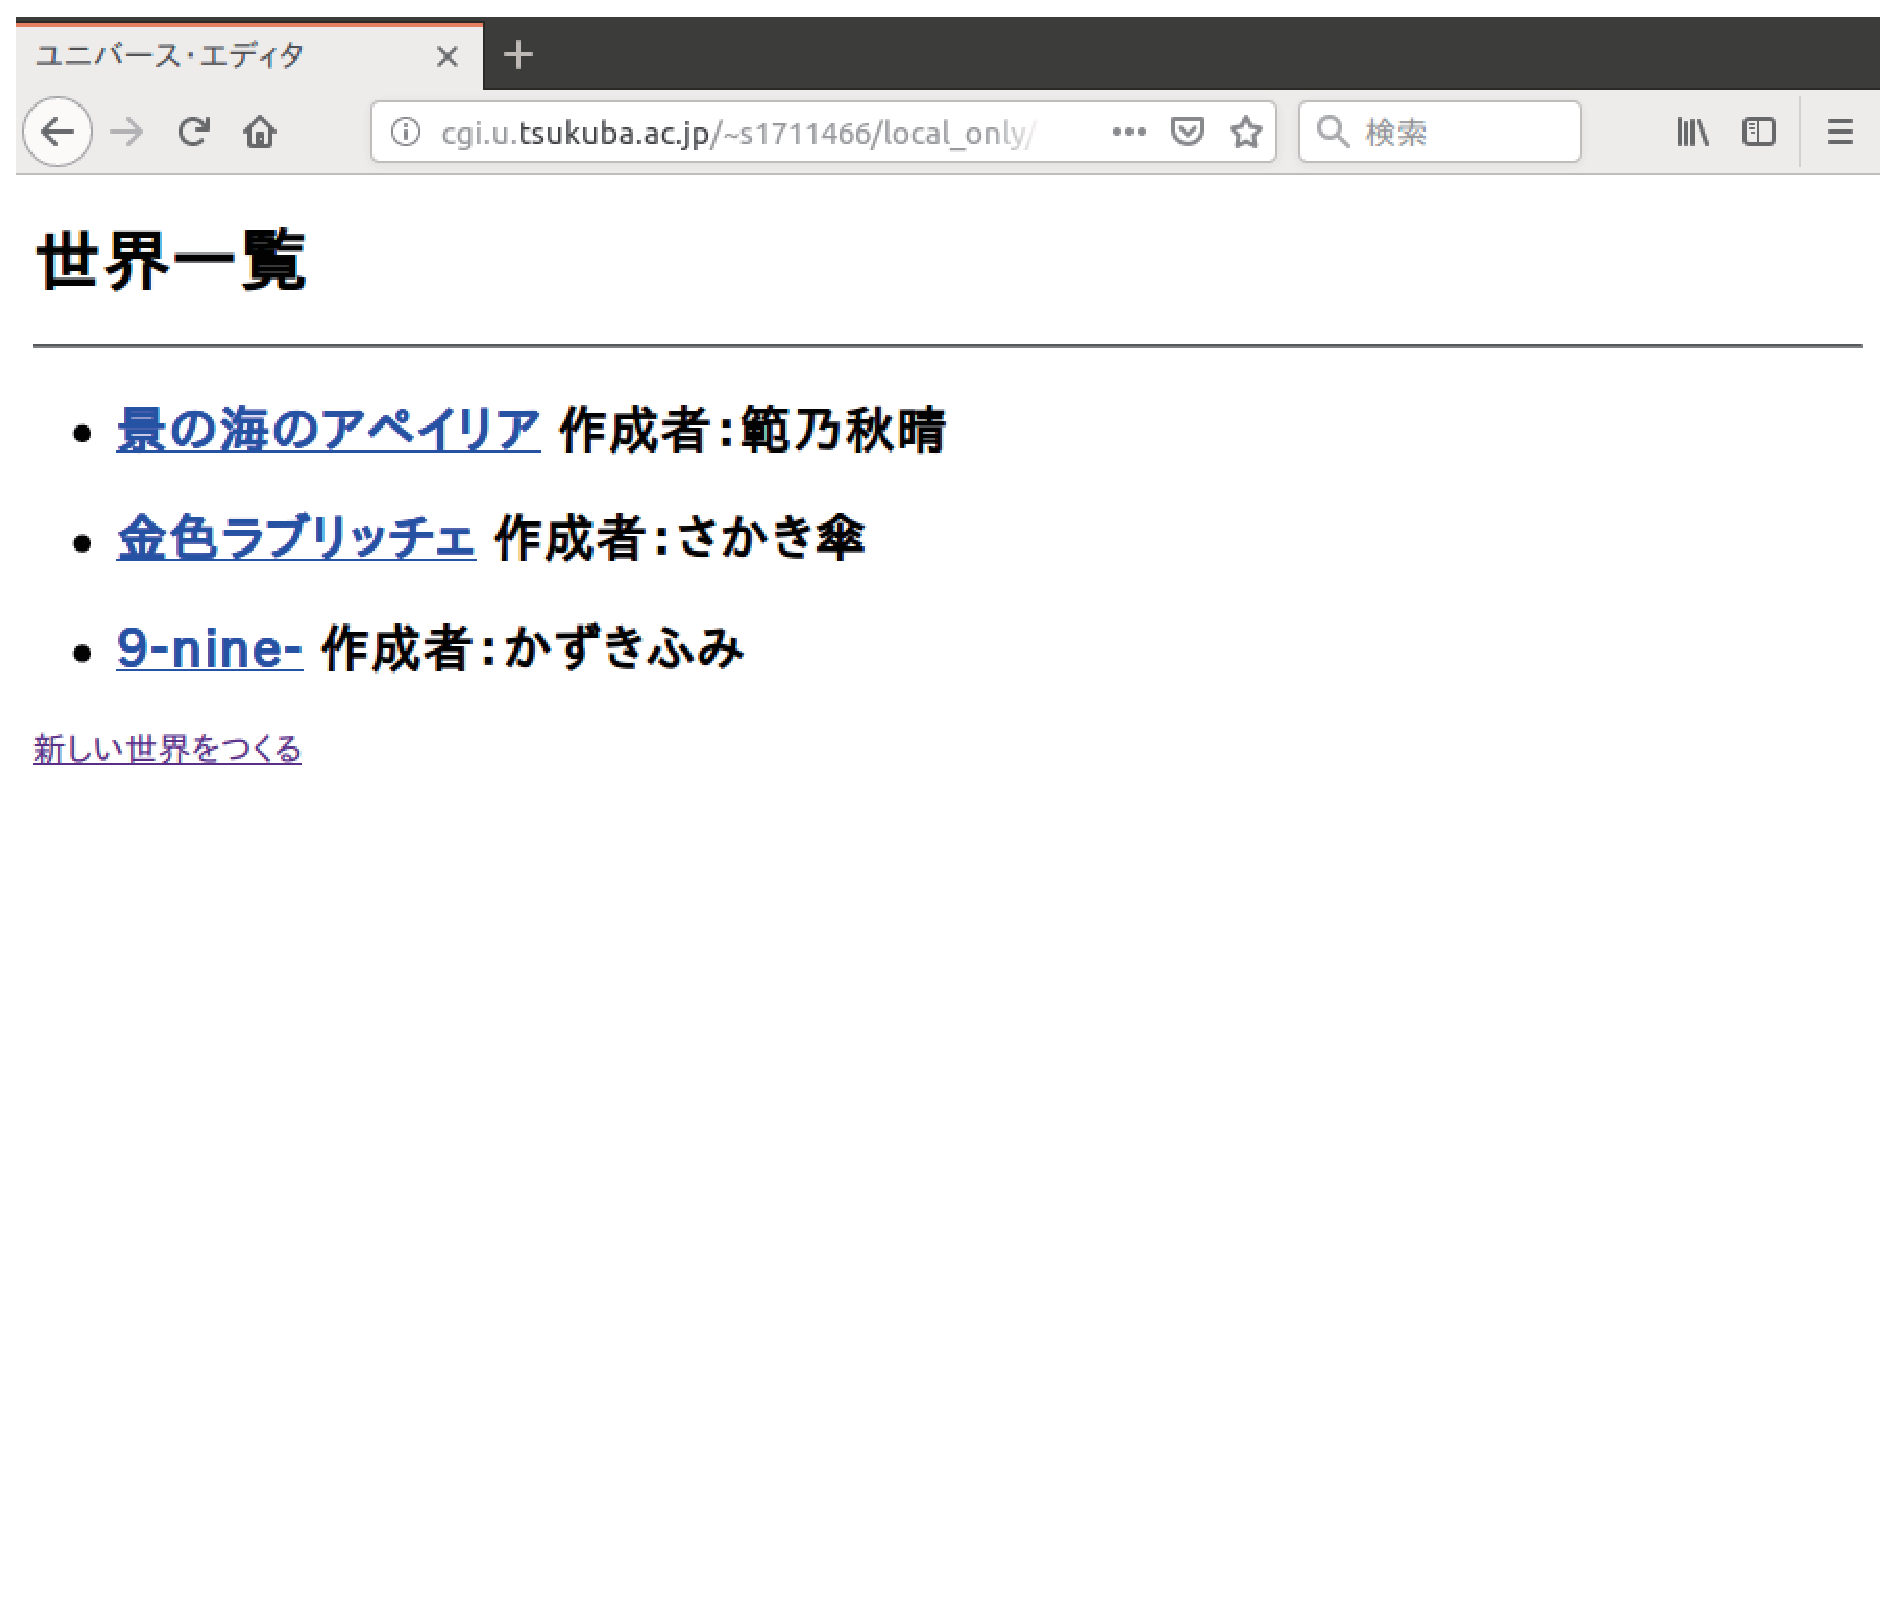
\includegraphics[width=7.0cm]{10-3-1.eps}
          \hspace{1.6cm} [1]ホーム画面
        \end{center}
      \end{minipage}

      % 2 
      \begin{minipage}{0.53\hsize}
        \begin{center}
          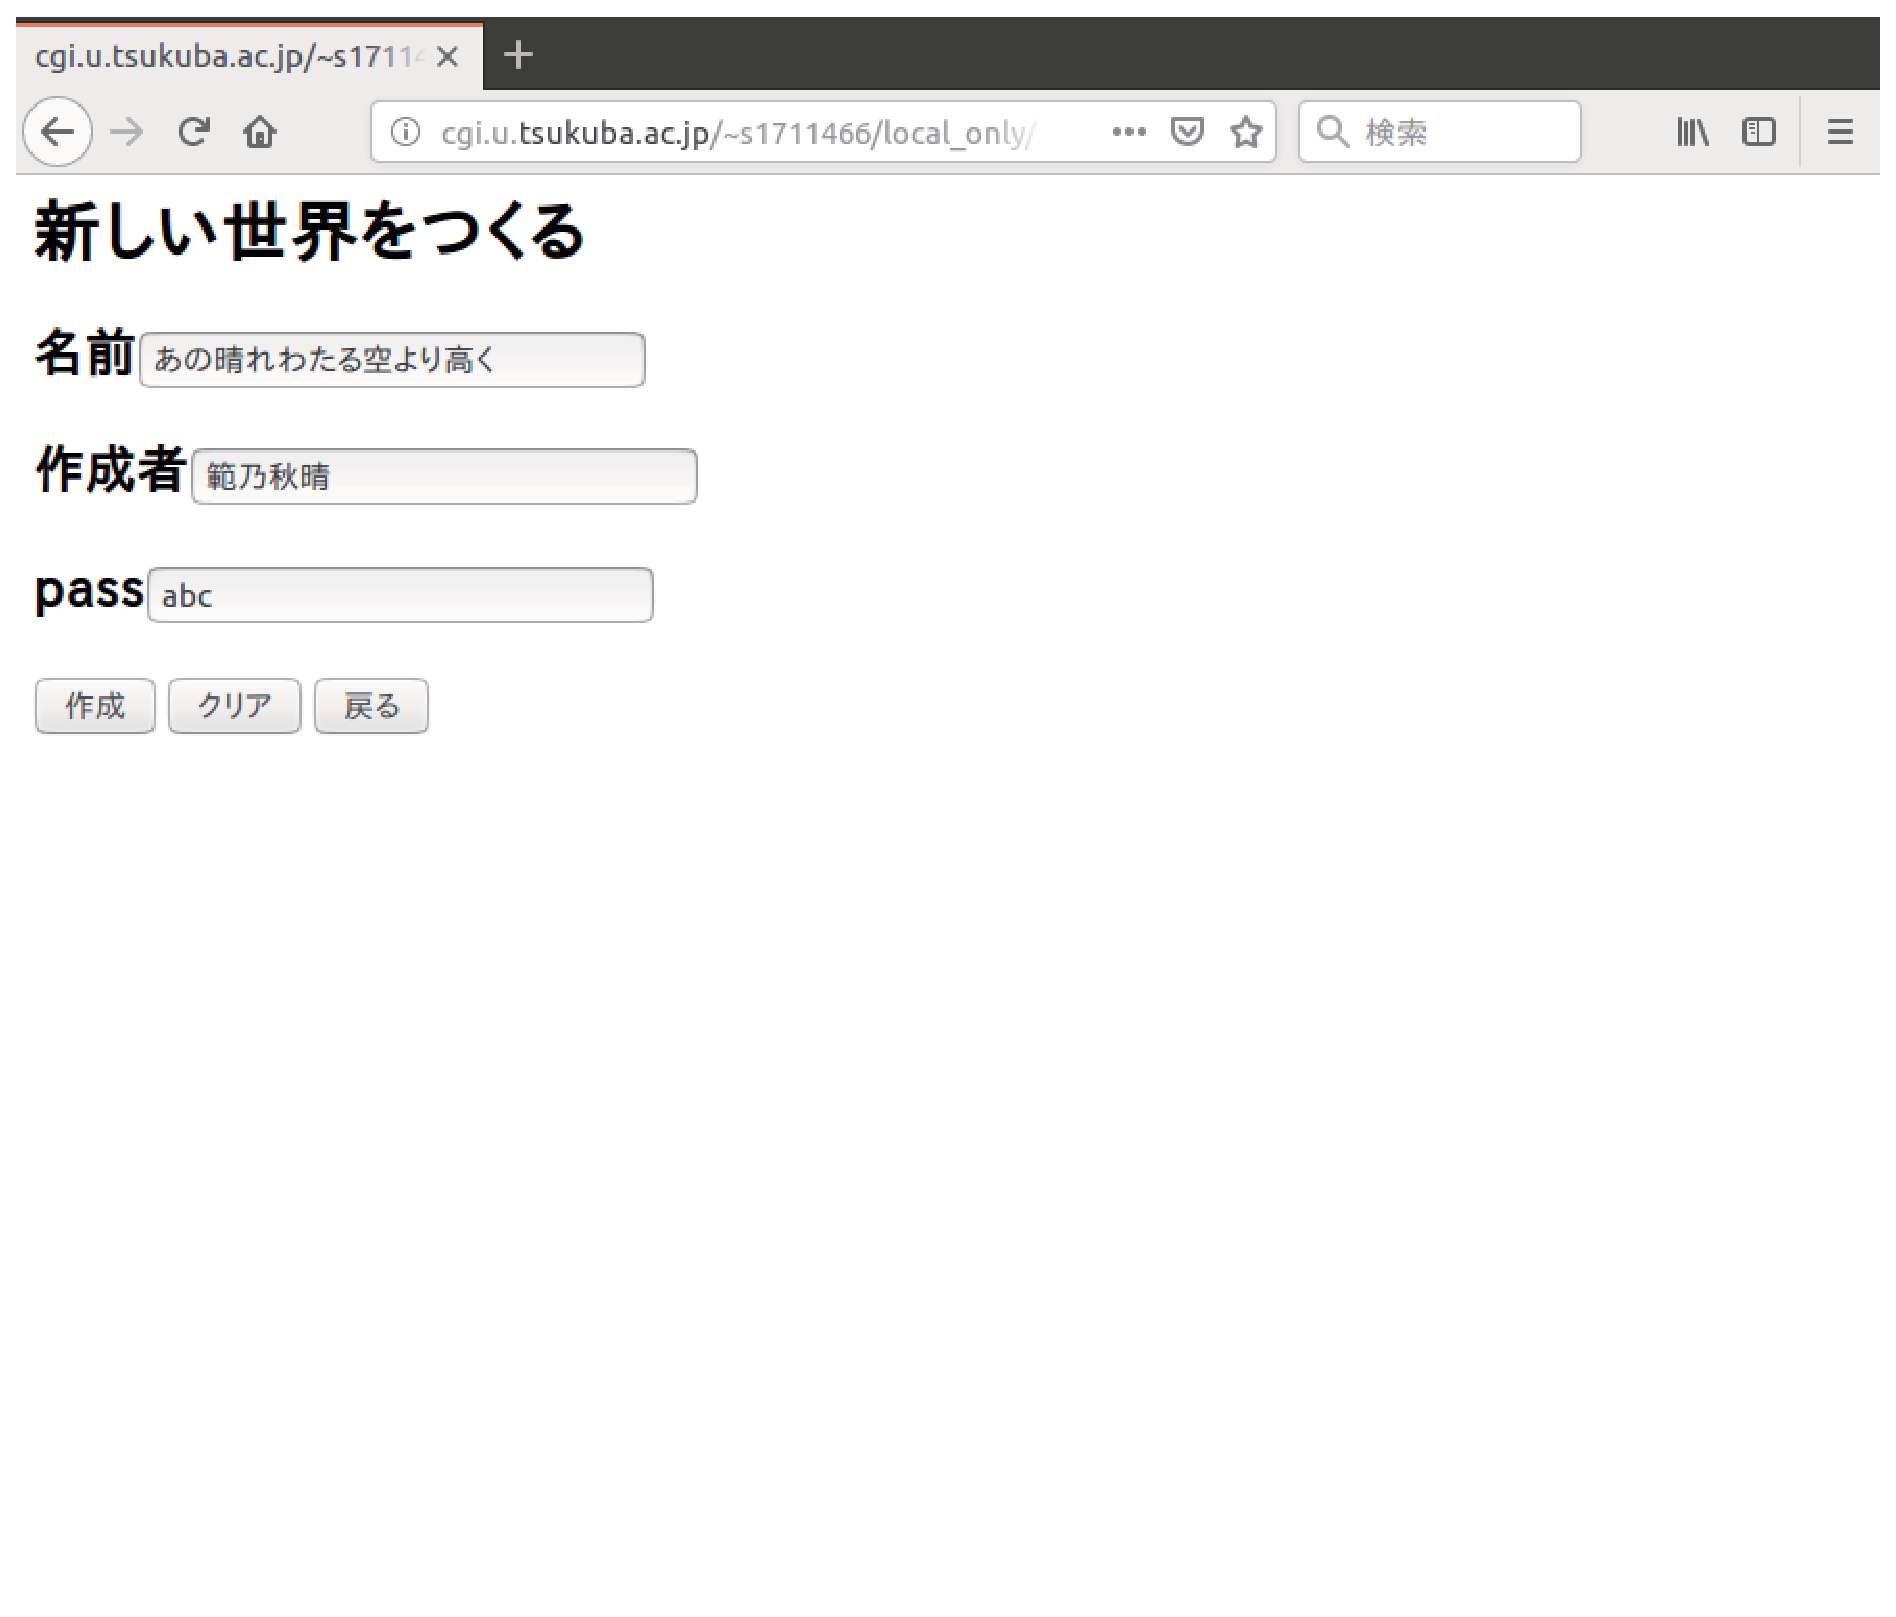
\includegraphics[width=7.0cm]{10-3-2.eps}
          \hspace{1.6cm} [2]新しい世界をつくる
        \end{center}
      \end{minipage}

      \begin{minipage}{0.55\hsize}
        \vspace{90mm}
      \end{minipage} \\
 
      % 3
      \begin{minipage}{0.53\hsize}
        \begin{center}
          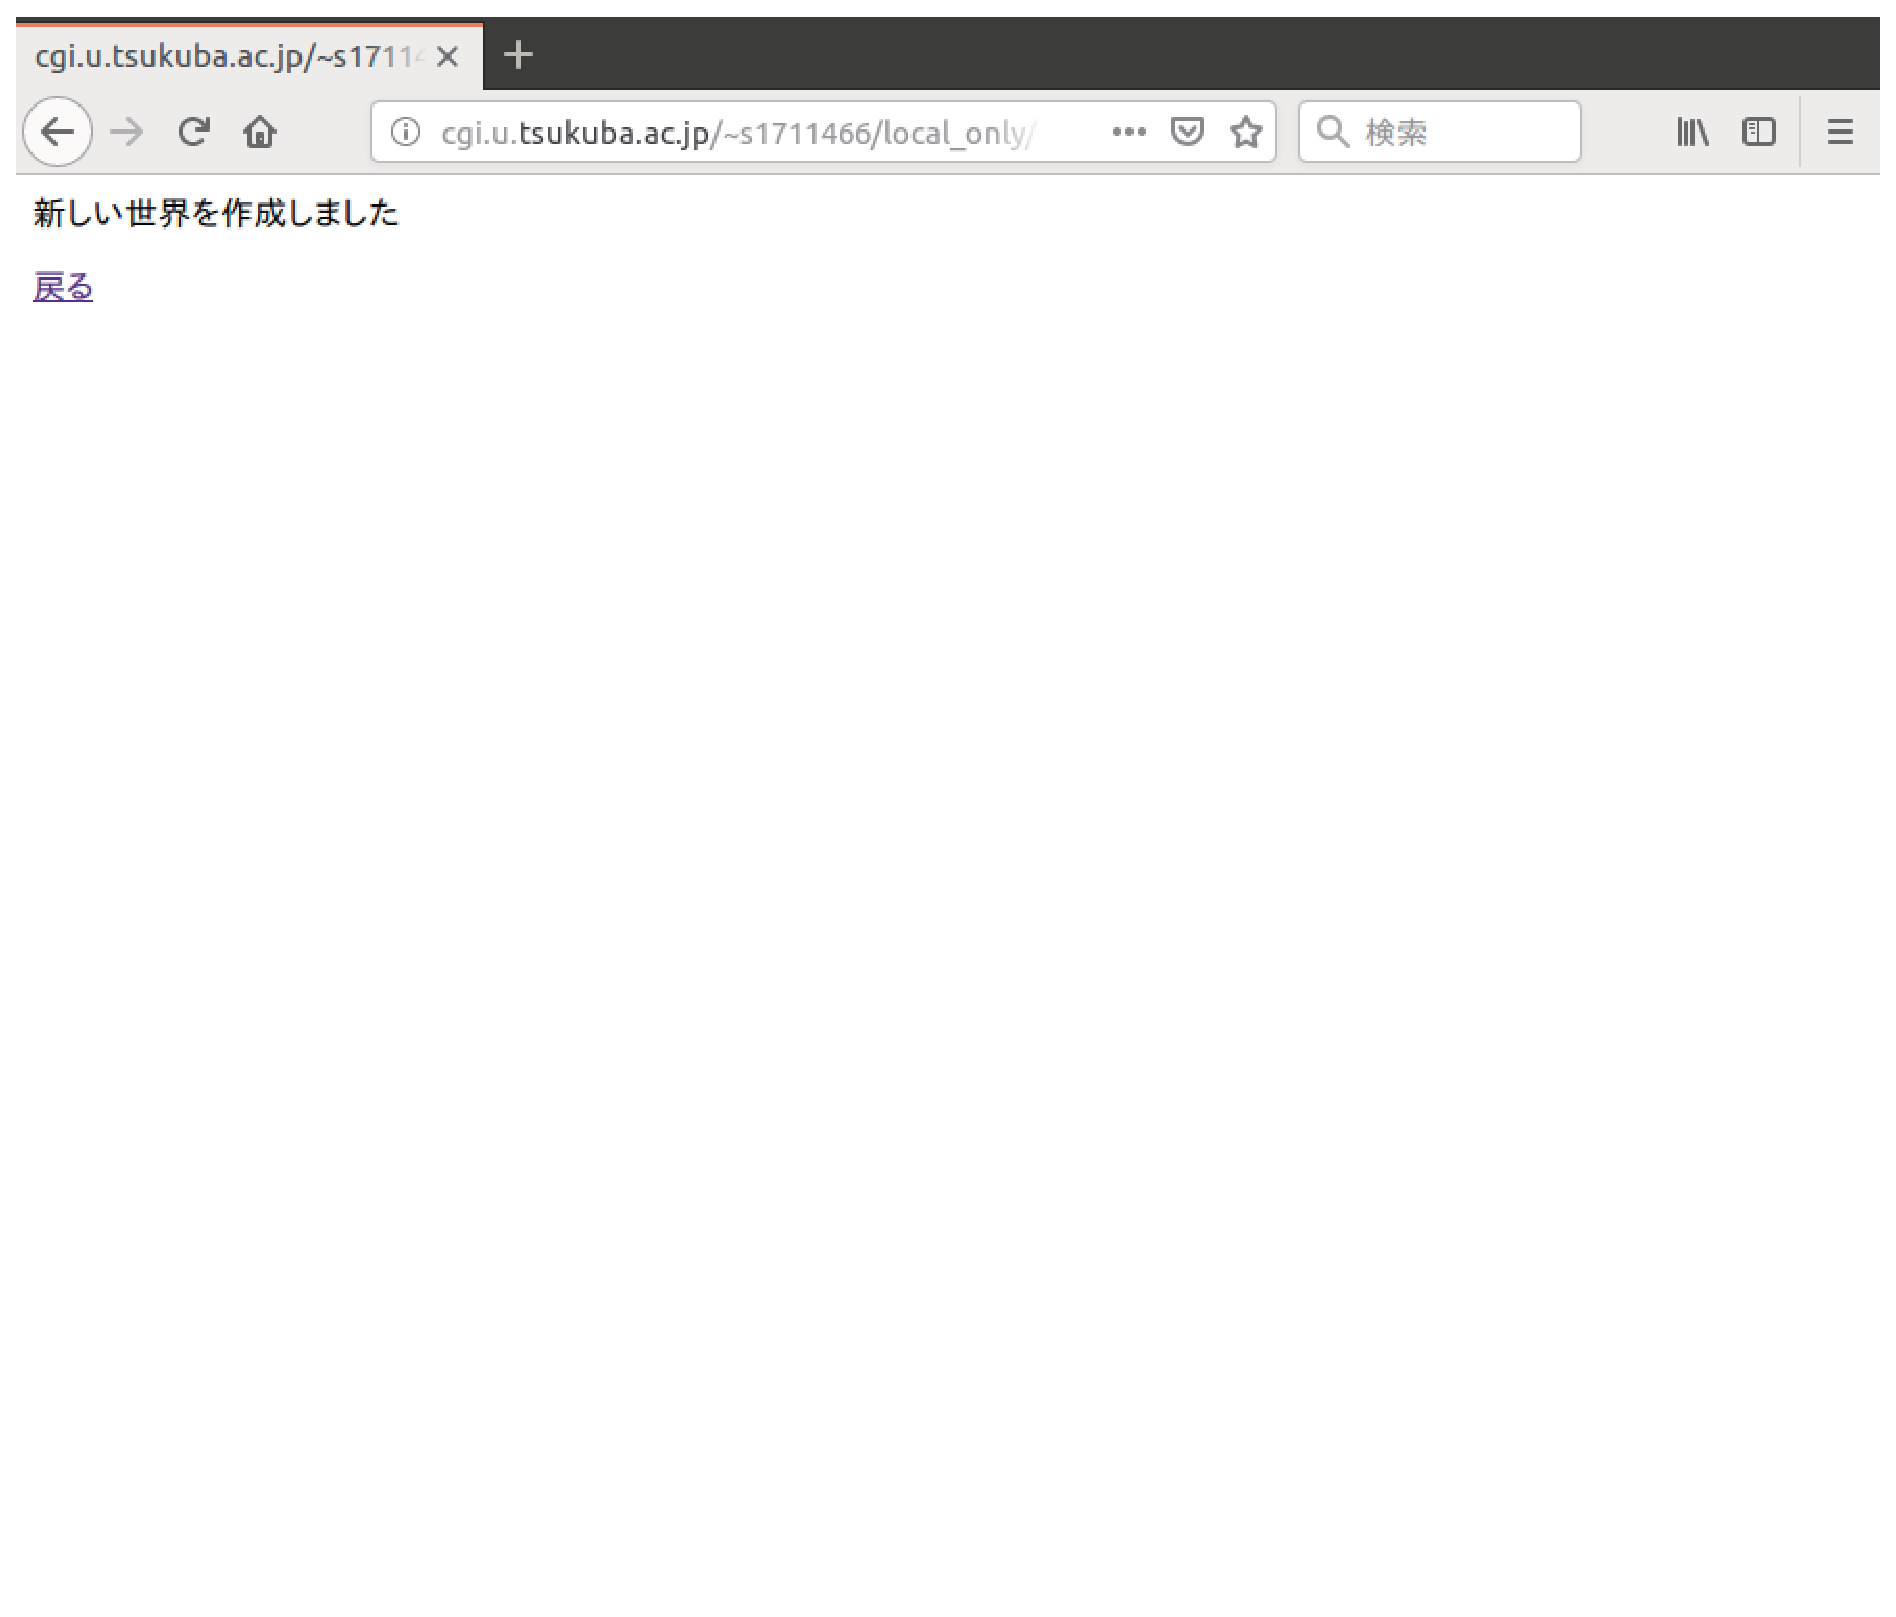
\includegraphics[width=7.0cm]{10-3-3.eps}
          \hspace{1.0cm} [3]作成完了
        \end{center}
      \end{minipage}

      % 4
      \begin{minipage}{0.53\hsize}
        \begin{center}
          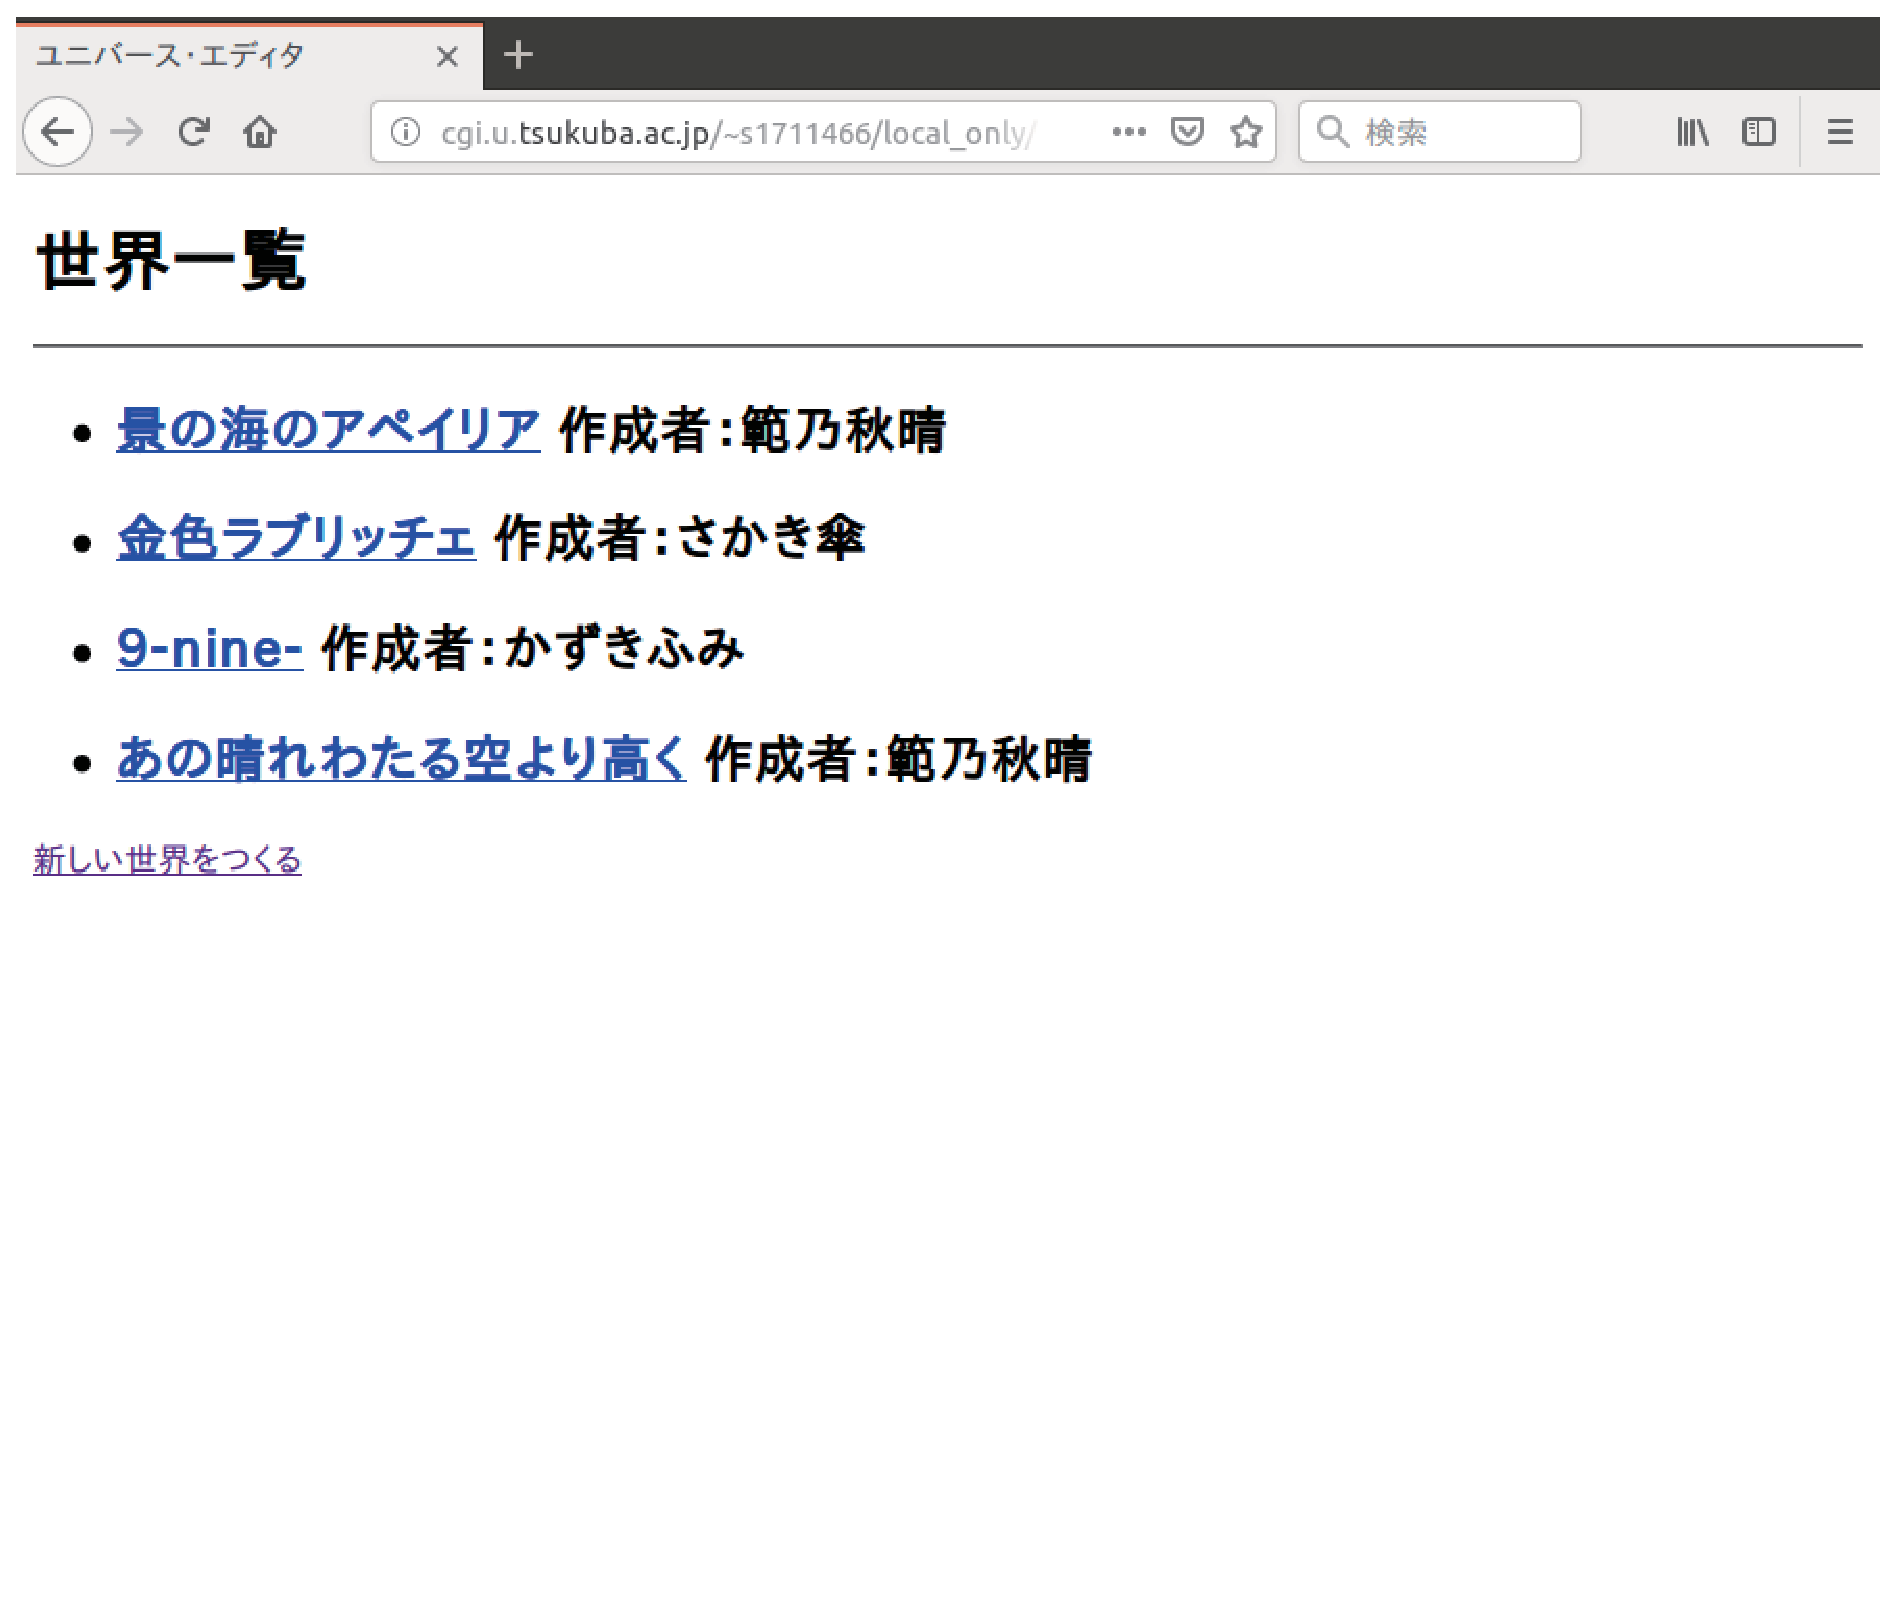
\includegraphics[width=7.0cm]{10-3-4.eps}
          \hspace{1.6cm} [4]新しい世界が追加されたホーム画面
        \end{center}
      \end{minipage}\\

    \end{tabular}
    \caption{世界の作成関連の動作画面}
    \label{fig:a}
  \end{center}
\end{figure}

\begin{figure}[htbp]
  \begin{center}
    \begin{tabular}{c}

      % 1 ホーム画面
      \begin{minipage}{0.55\hsize}
        \begin{center}
          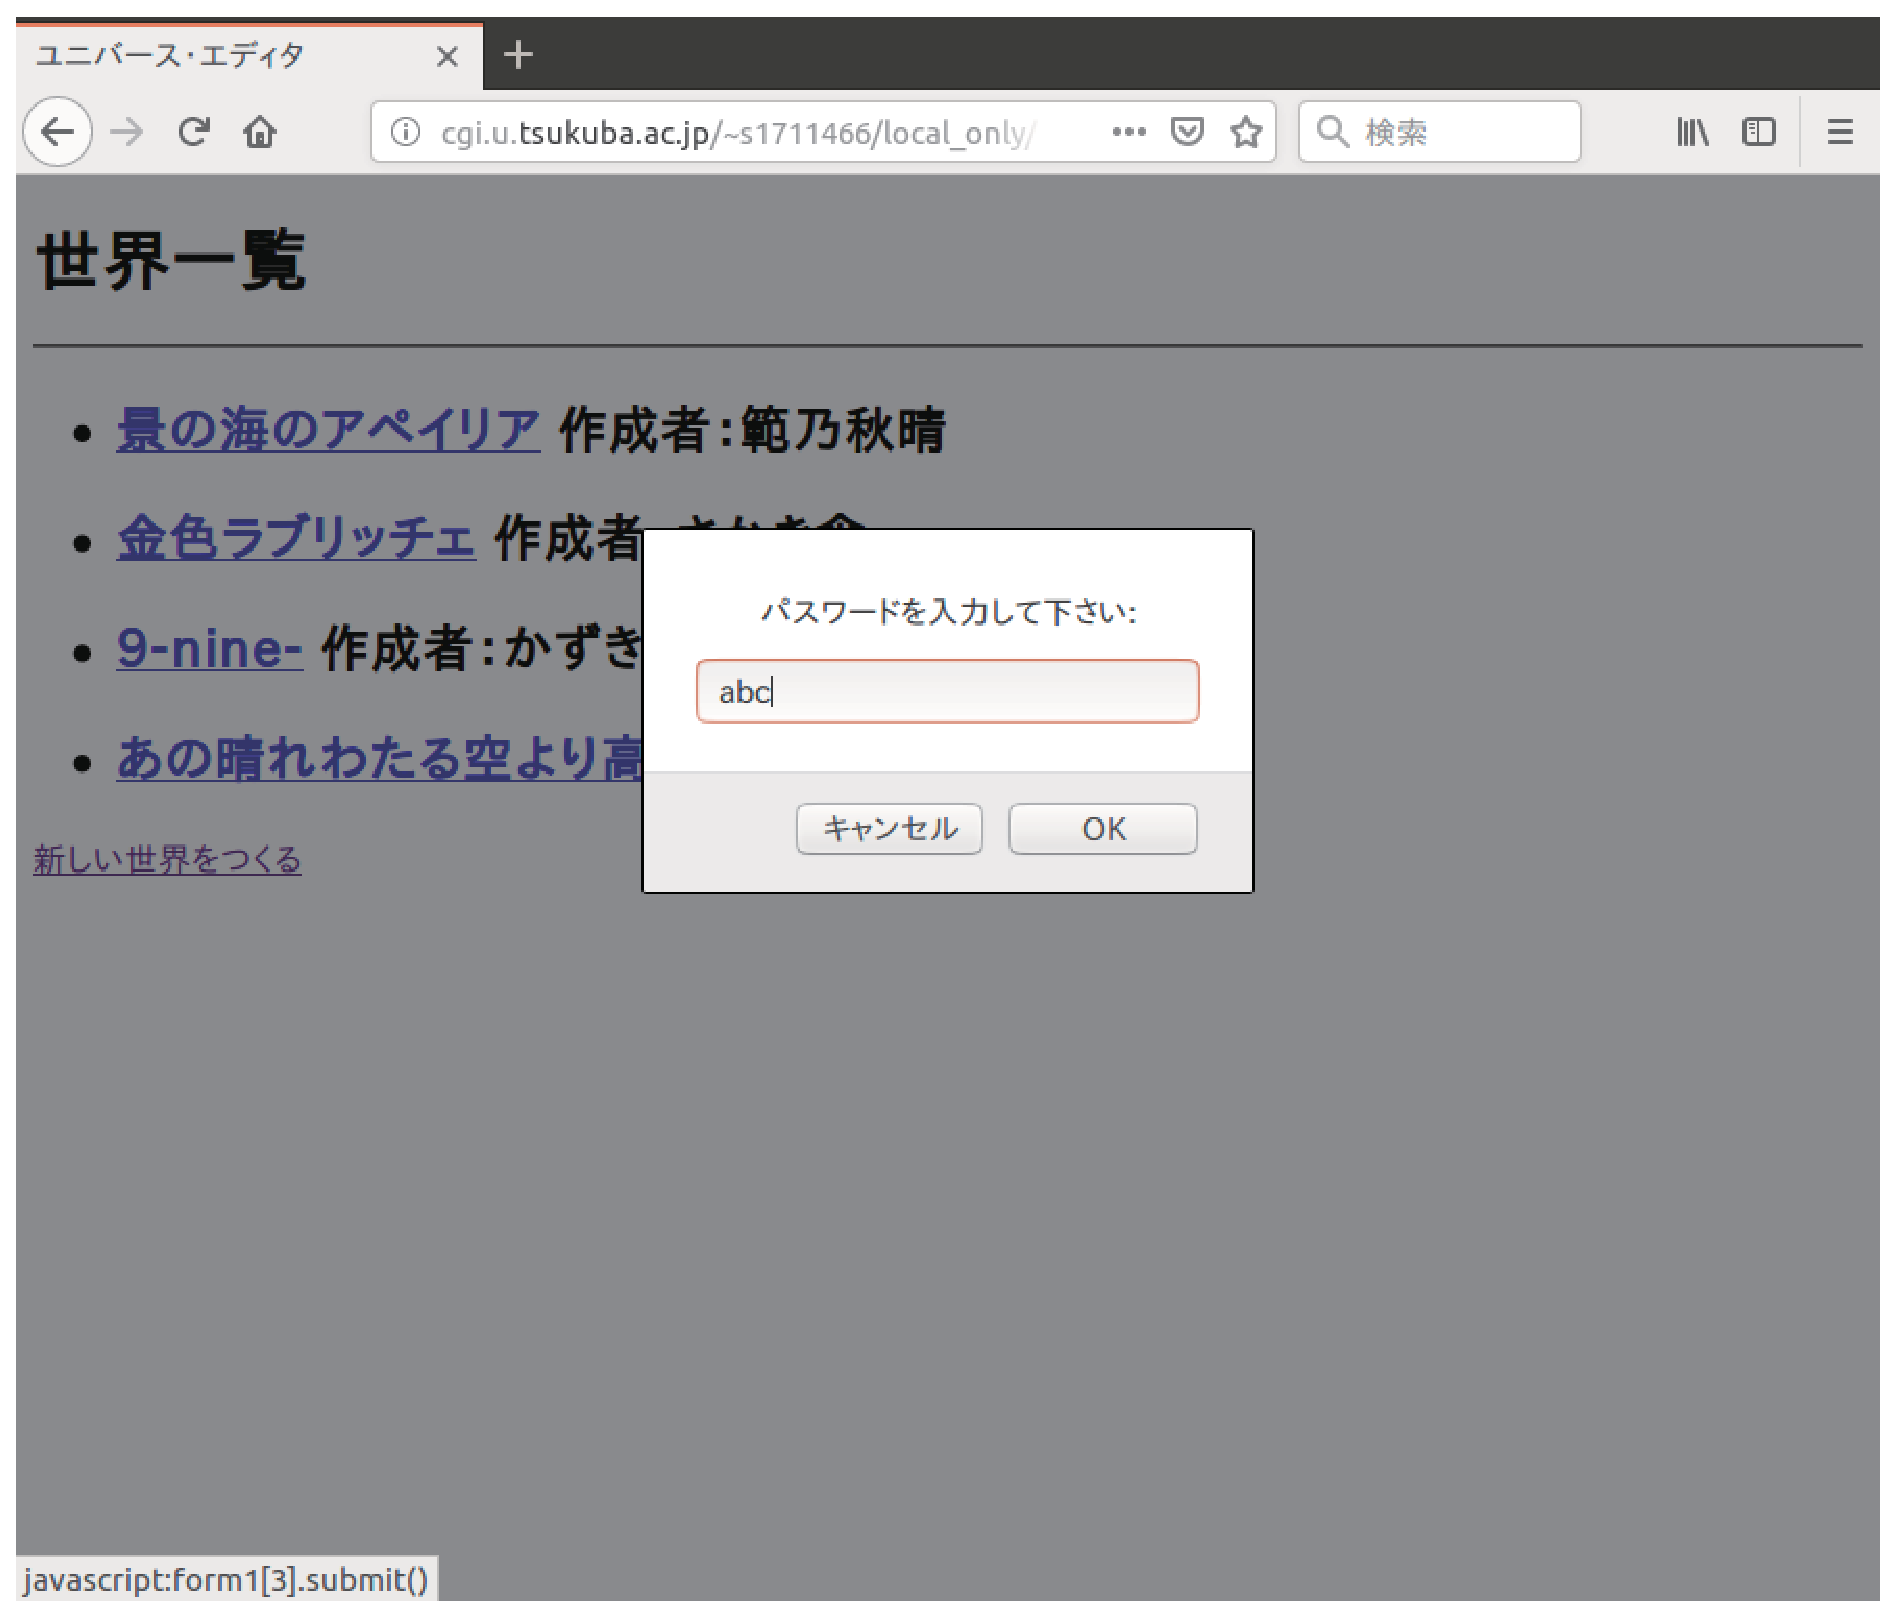
\includegraphics[width=7.0cm]{10-3-5.eps}
          \hspace{1.6cm} [1]パスワード要求
        \end{center}
      \end{minipage}

      % 2 
      \begin{minipage}{0.55\hsize}
        \begin{center}
          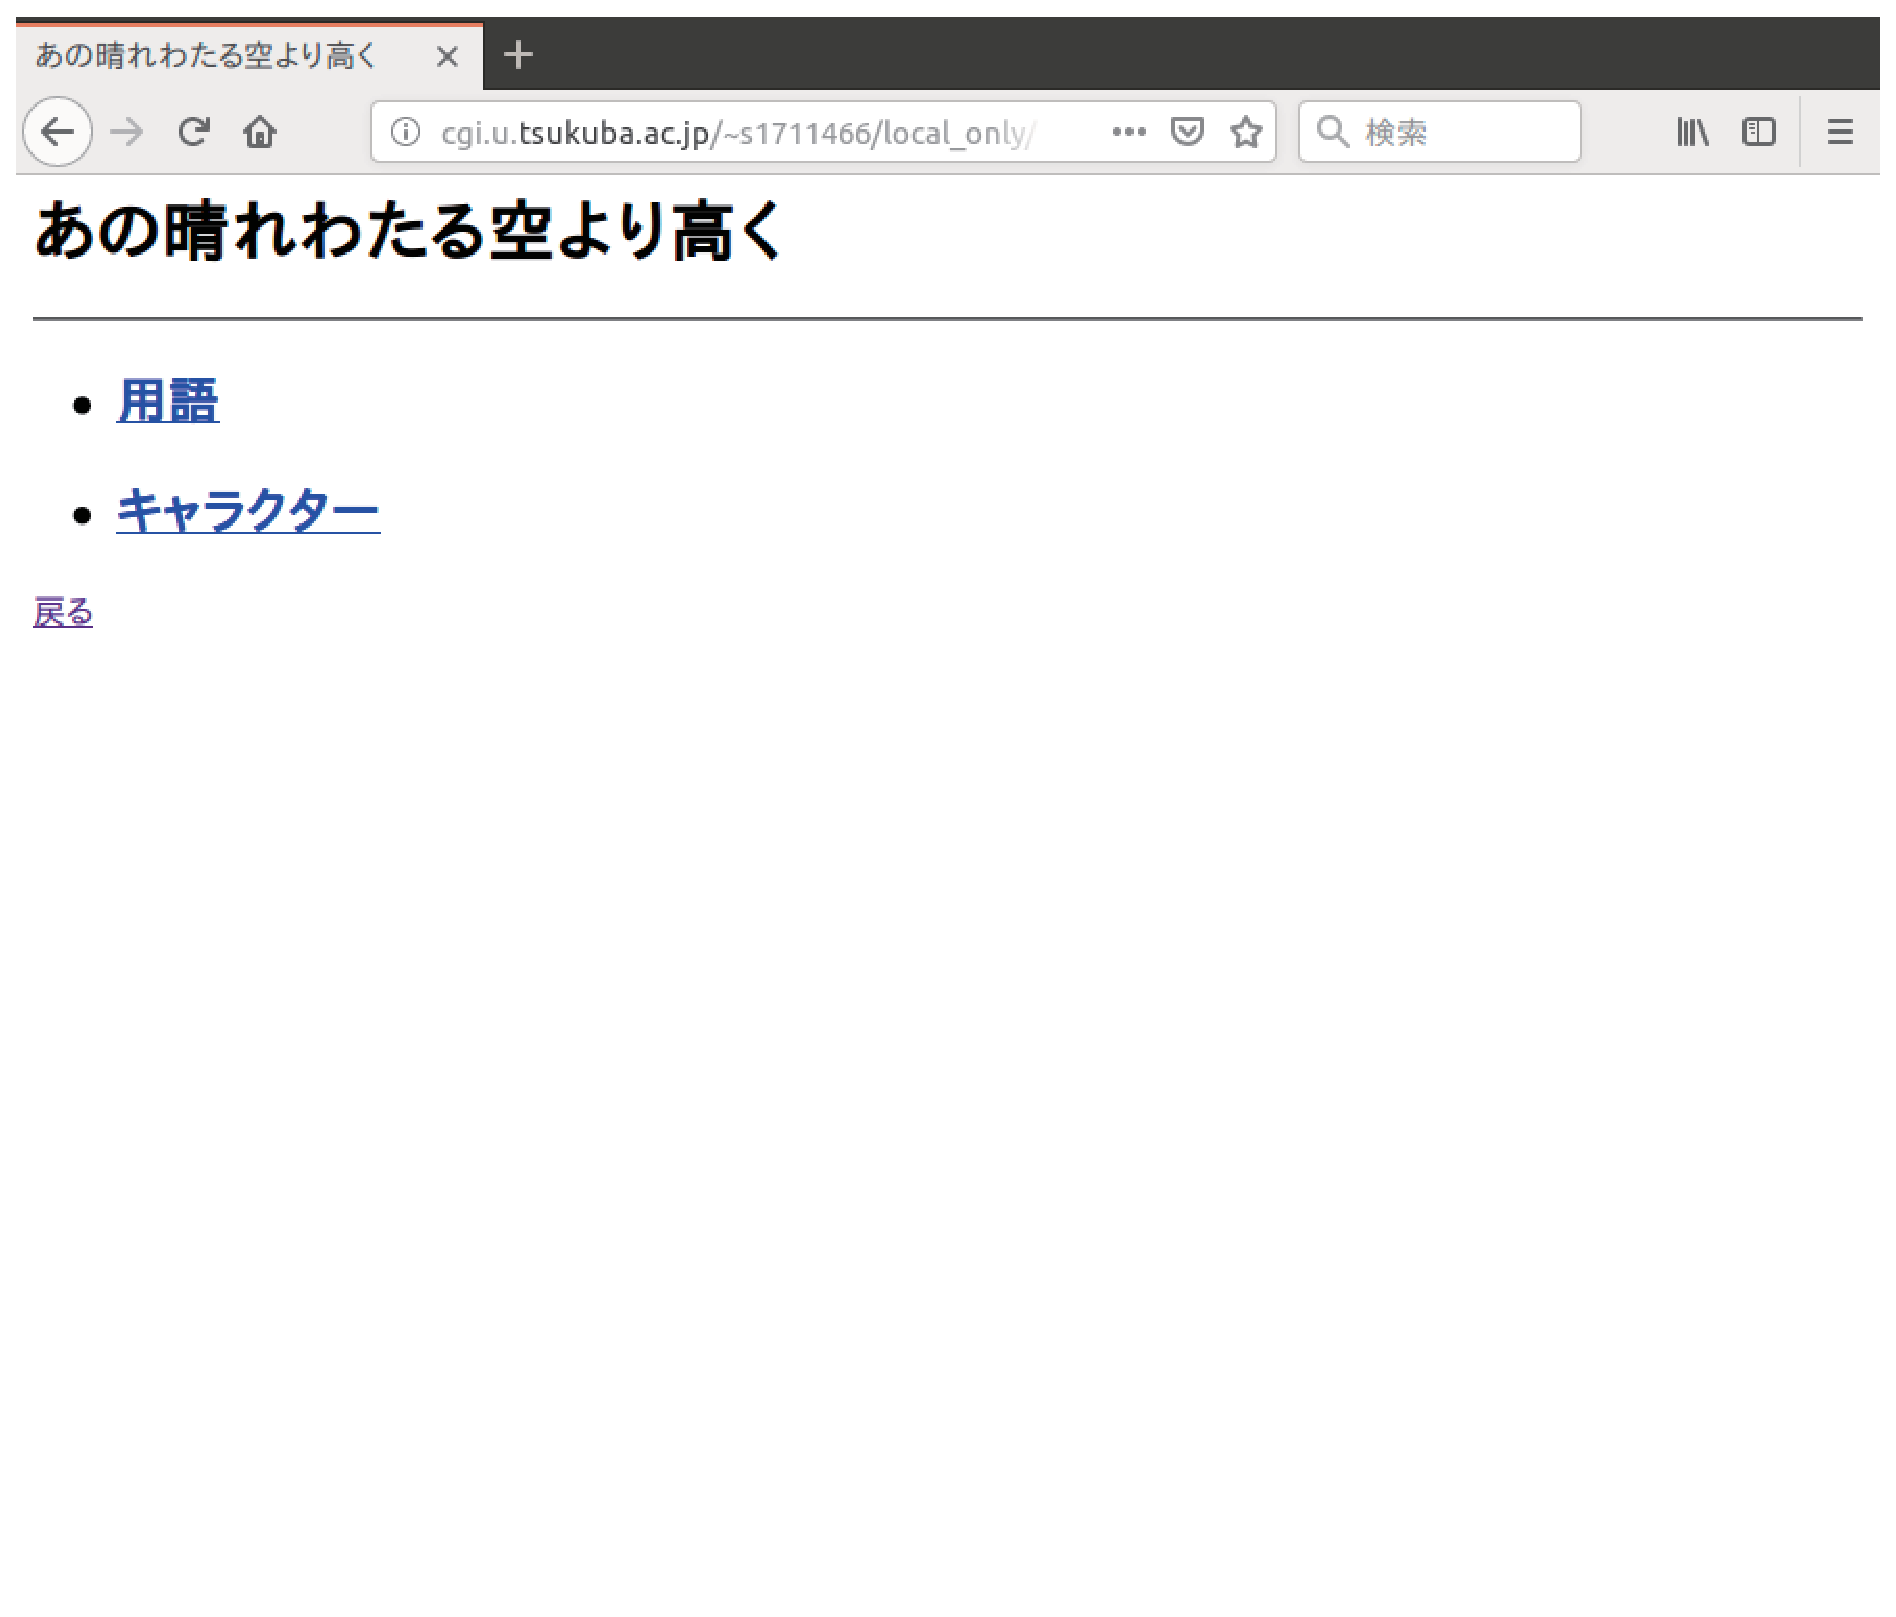
\includegraphics[width=6.7cm]{10-3-6.eps}
          \hspace{1.6cm} [2]世界の個別ページ
        \end{center}
      \end{minipage}

    \end{tabular}
    \caption{世界関係の動作画面}
    \label{fig:b}
  \end{center}
\end{figure}

\begin{figure}[htbp]
  \begin{center}
    \begin{tabular}{c}

      % 1 ホーム画面
      \begin{minipage}{0.55\hsize}
        \begin{center}
          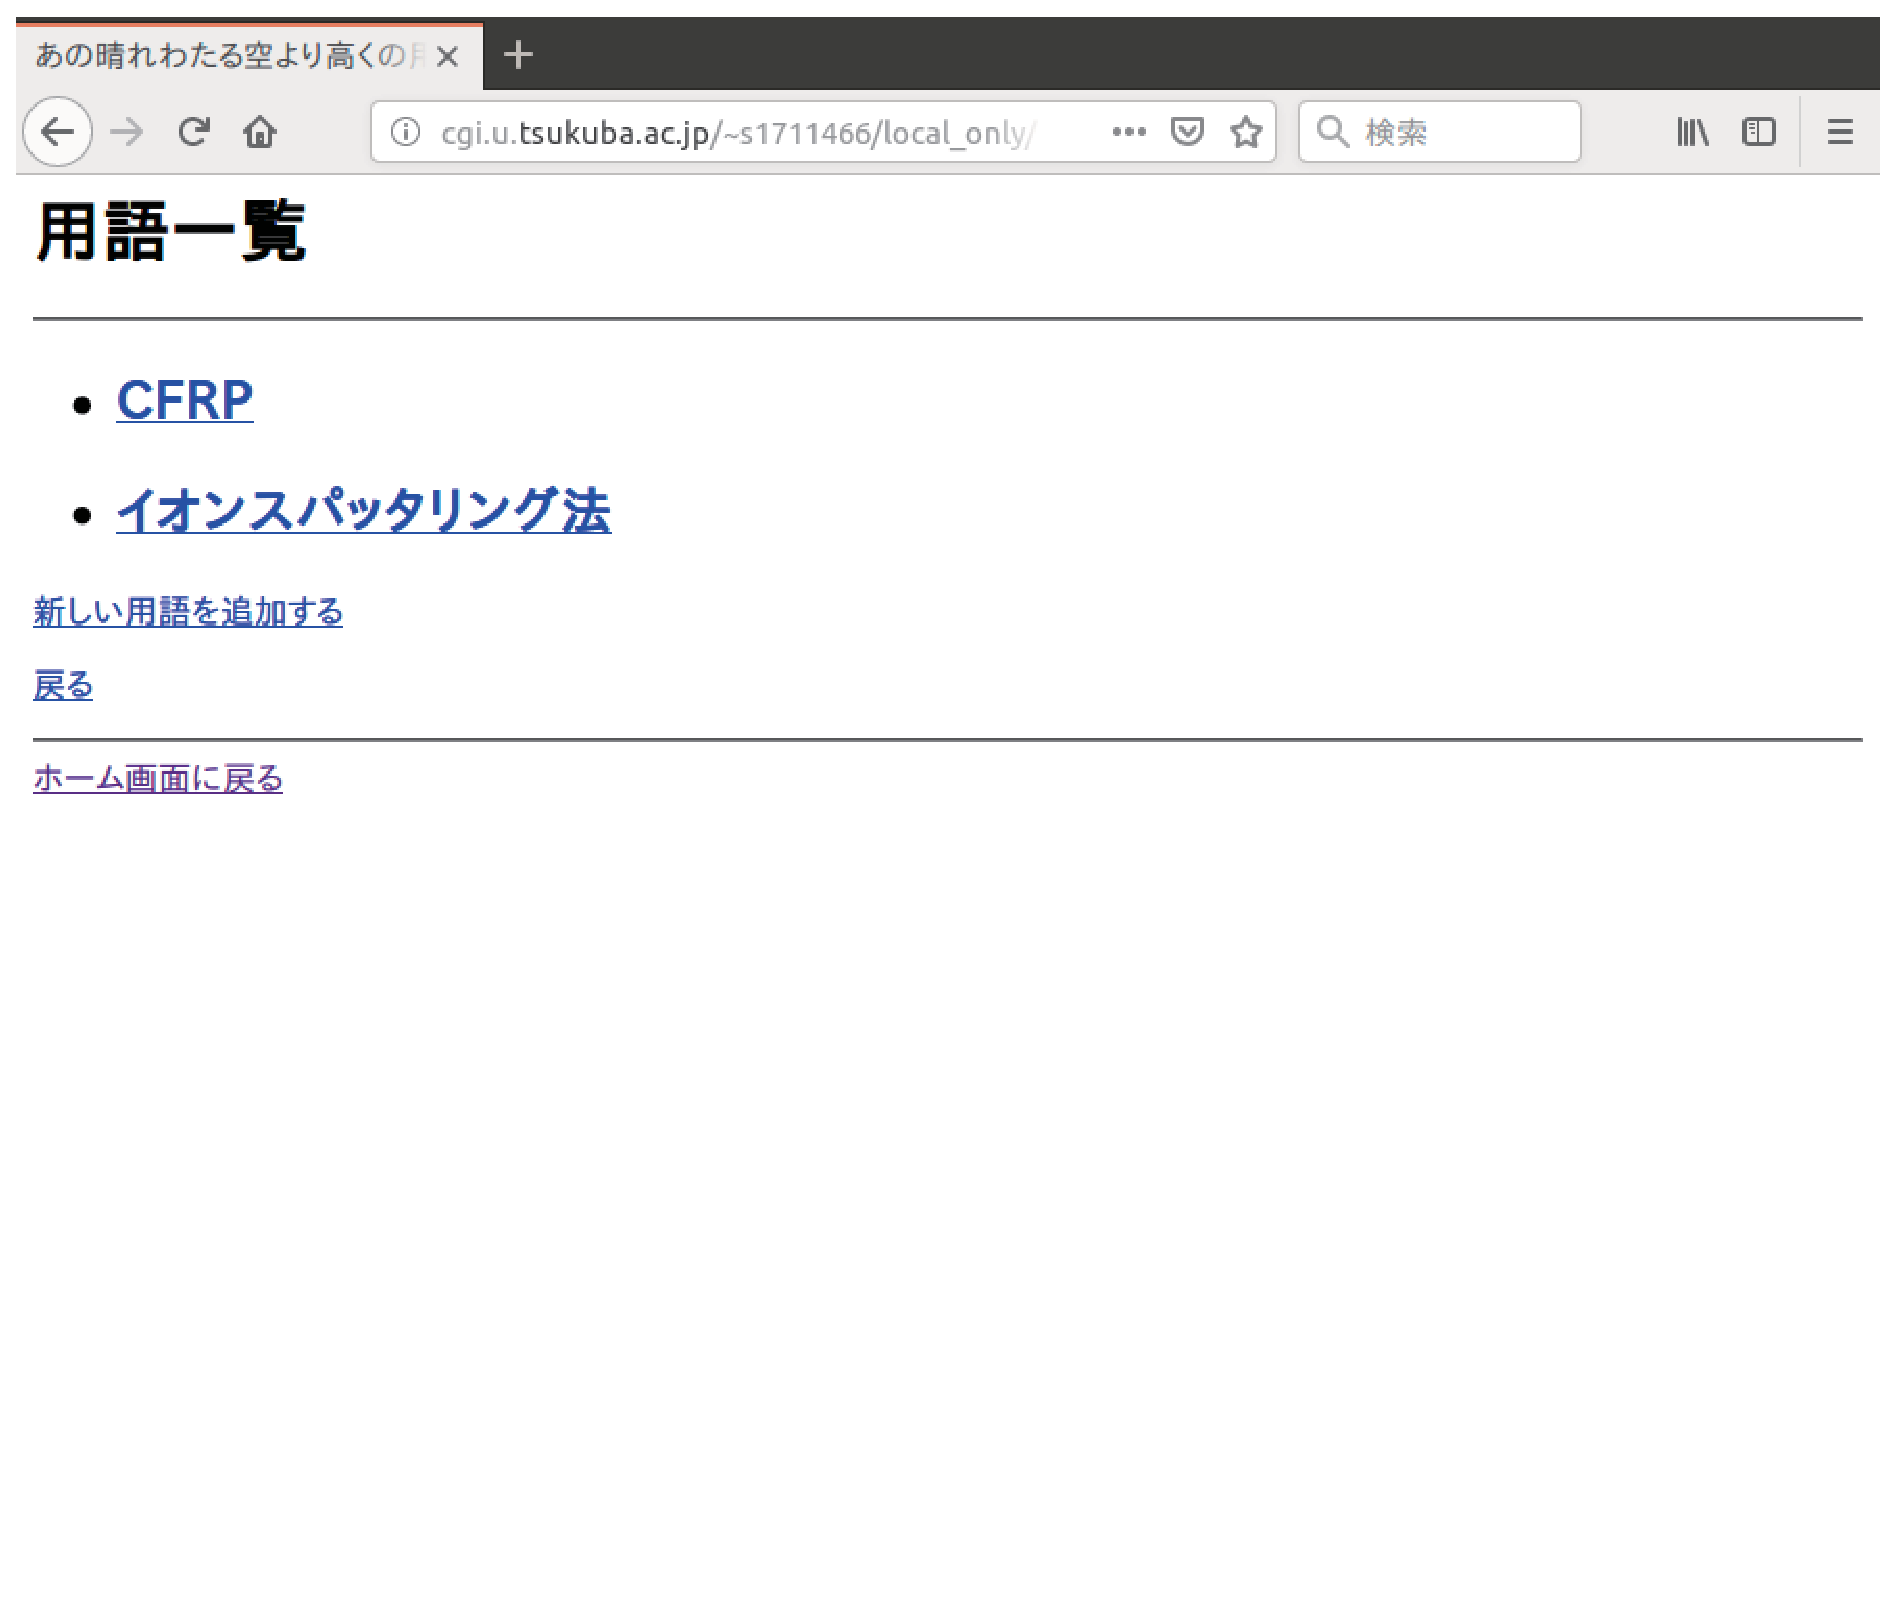
\includegraphics[width=7.0cm]{10-3-7.eps}
          \hspace{1.6cm} [1]用語一覧
        \end{center}
      \end{minipage}

      % 2 
      \begin{minipage}{0.55\hsize}
        \begin{center}
          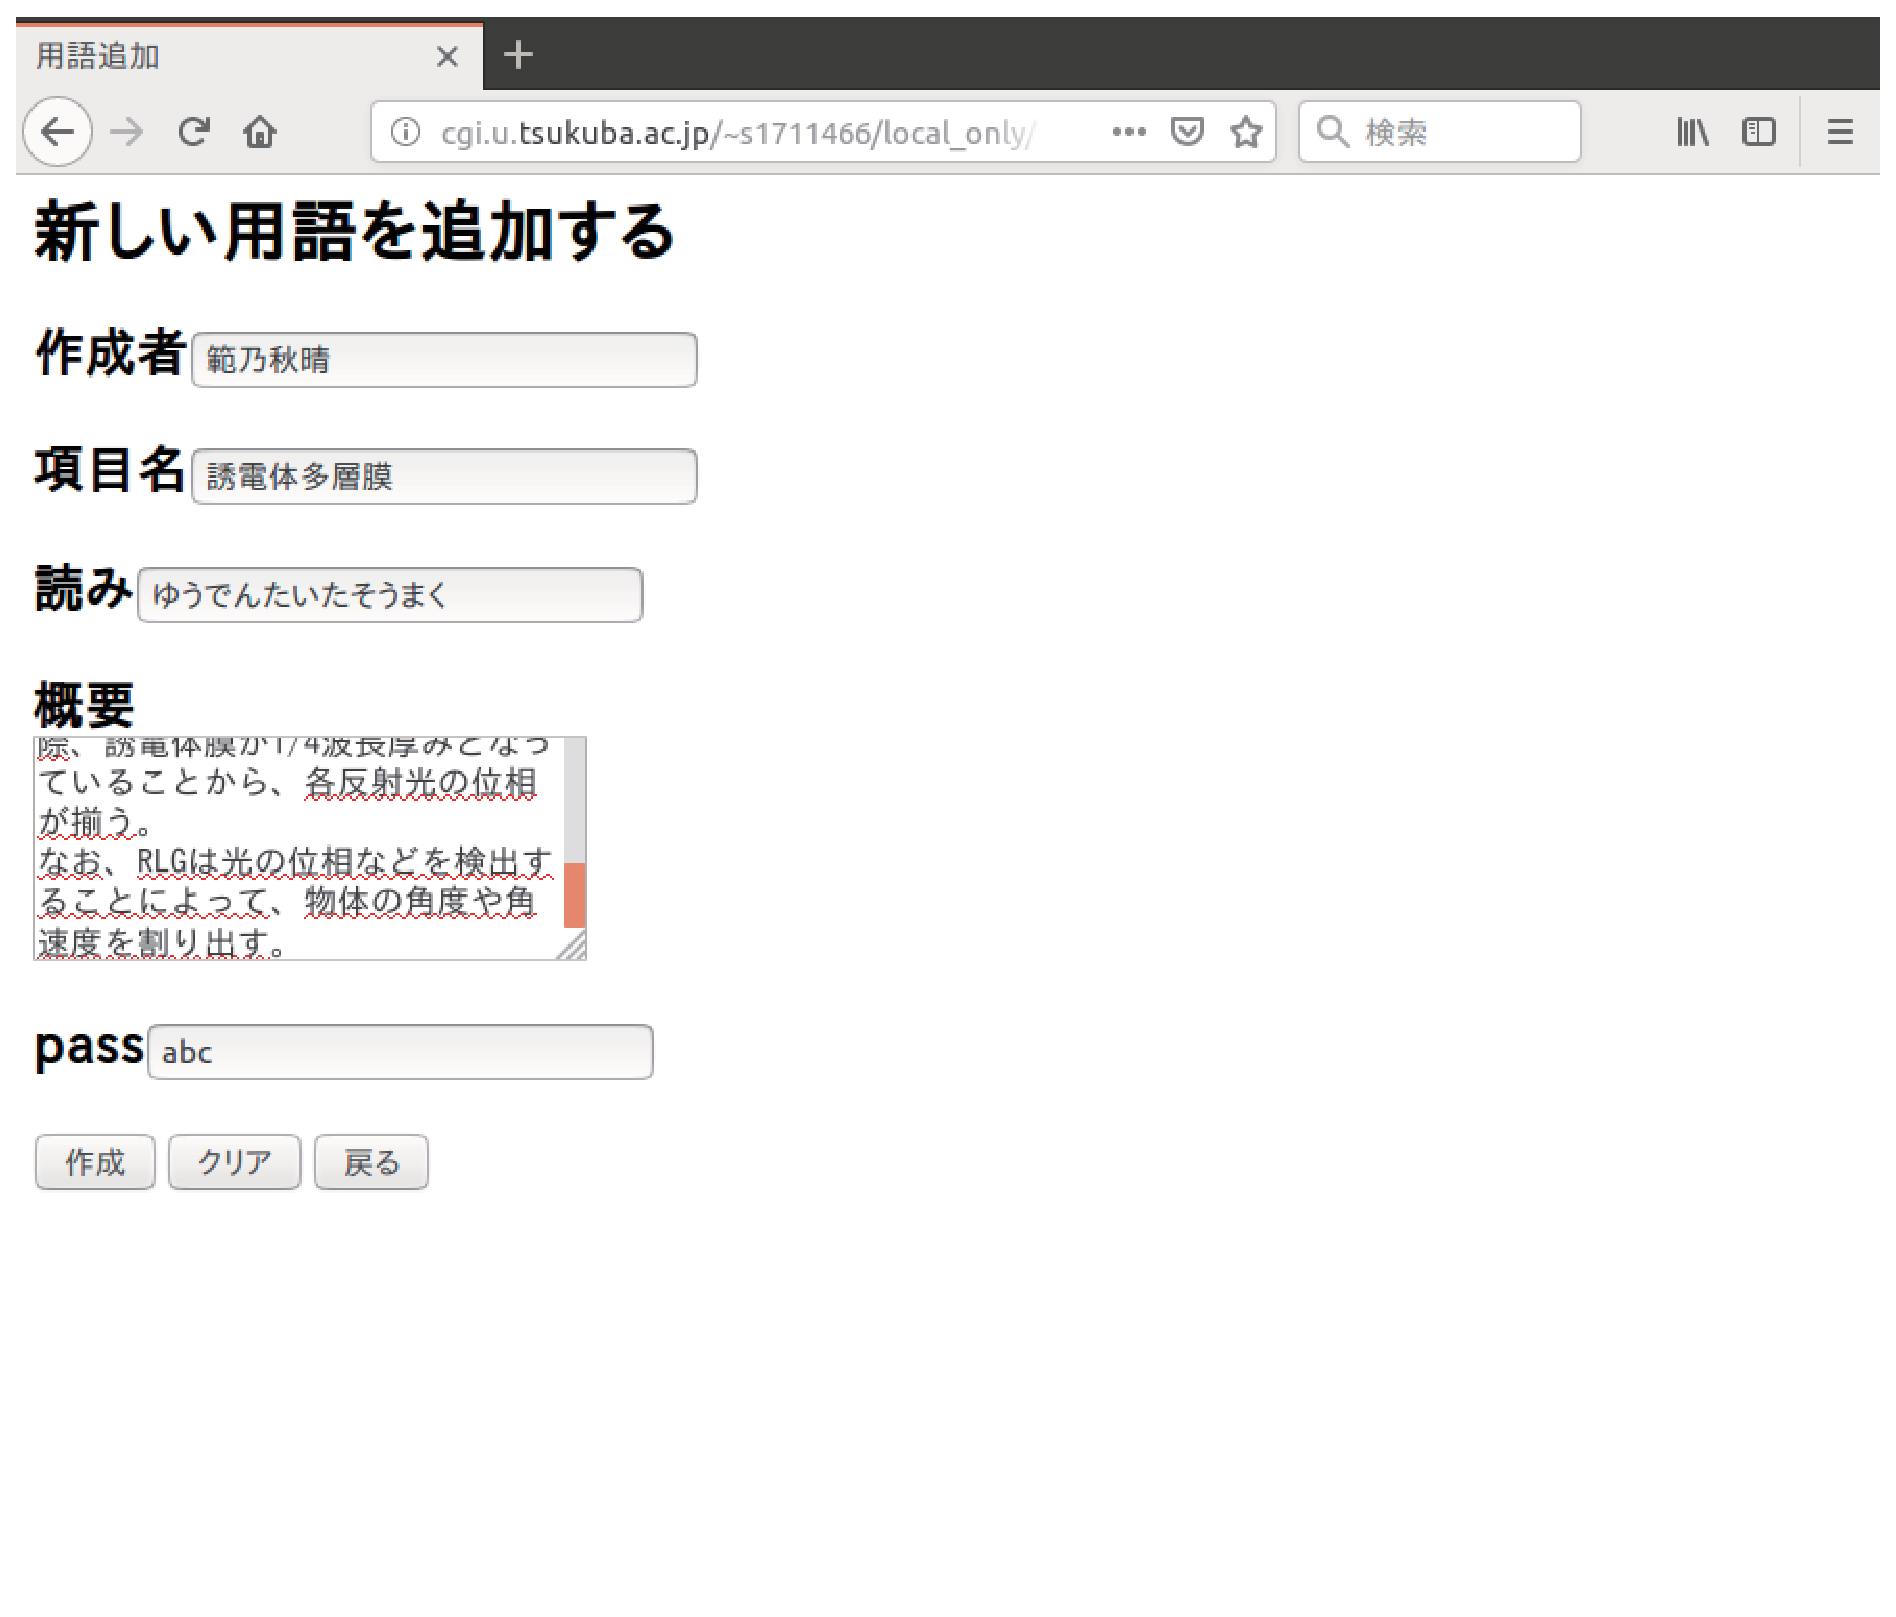
\includegraphics[width=6.7cm]{10-3-8.eps}
          \hspace{1.6cm} [2]新しい用語を追加する
        \end{center}
      \end{minipage}

      \begin{minipage}{0.55\hsize}
        \vspace{30mm}
      \end{minipage} \\
 
      % 3
      \begin{minipage}{0.5\hsize}
        \begin{center}
          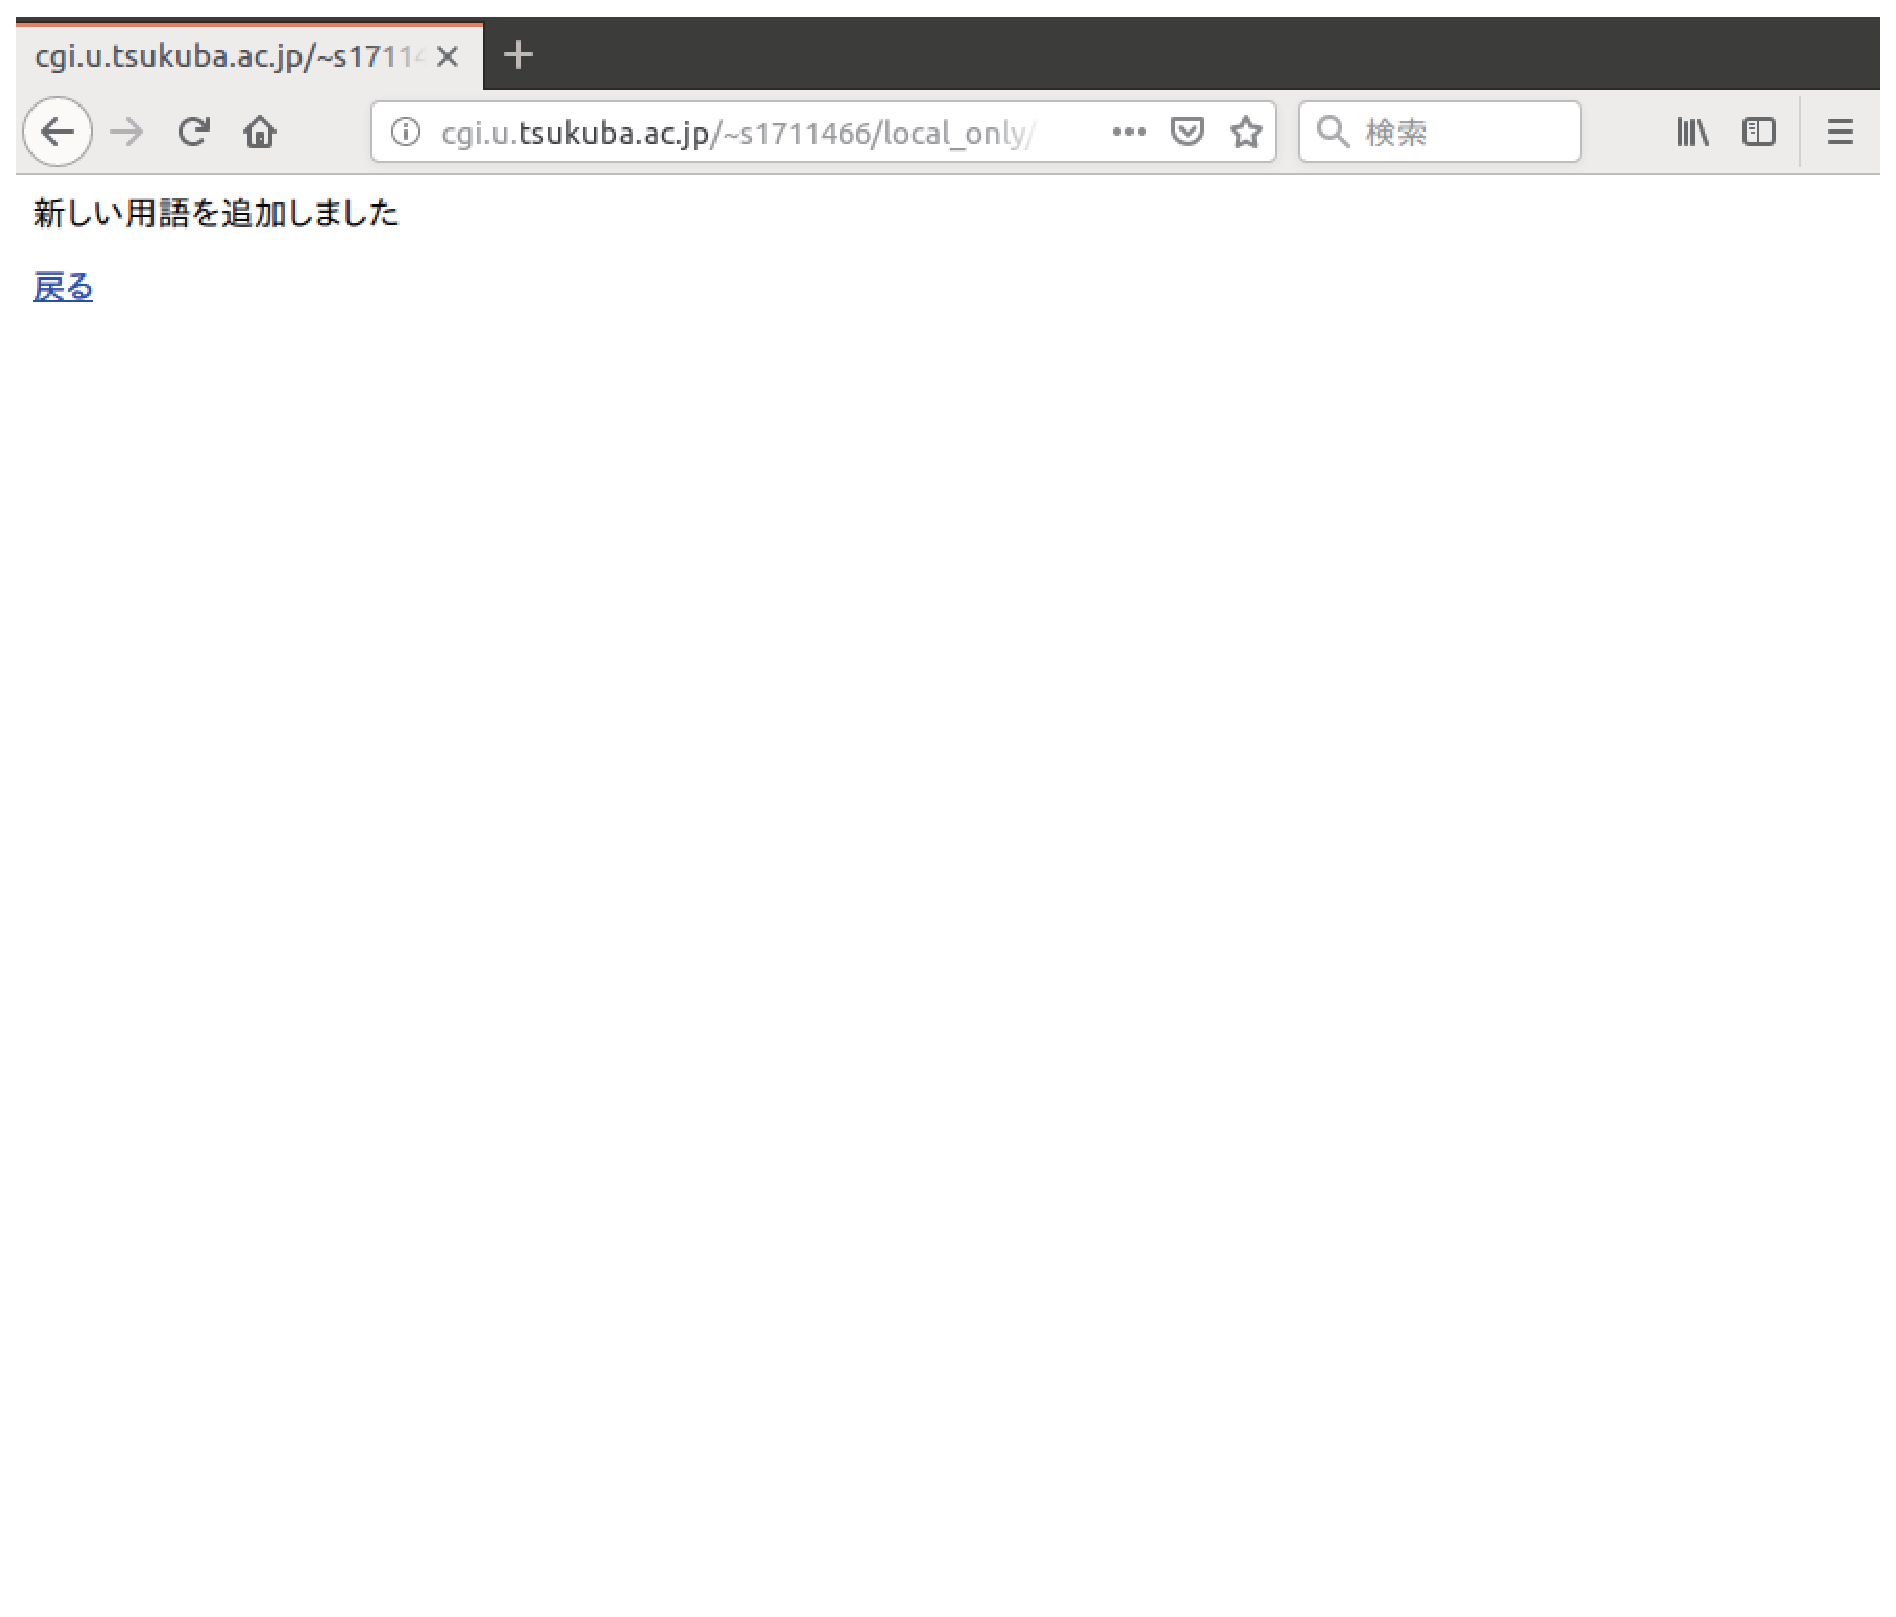
\includegraphics[width=6.7cm]{10-3-9.eps}
          \hspace{1.6cm} [3]追加完了
        \end{center}
      \end{minipage}

      % 4
      \begin{minipage}{0.55\hsize}
        \begin{center}
          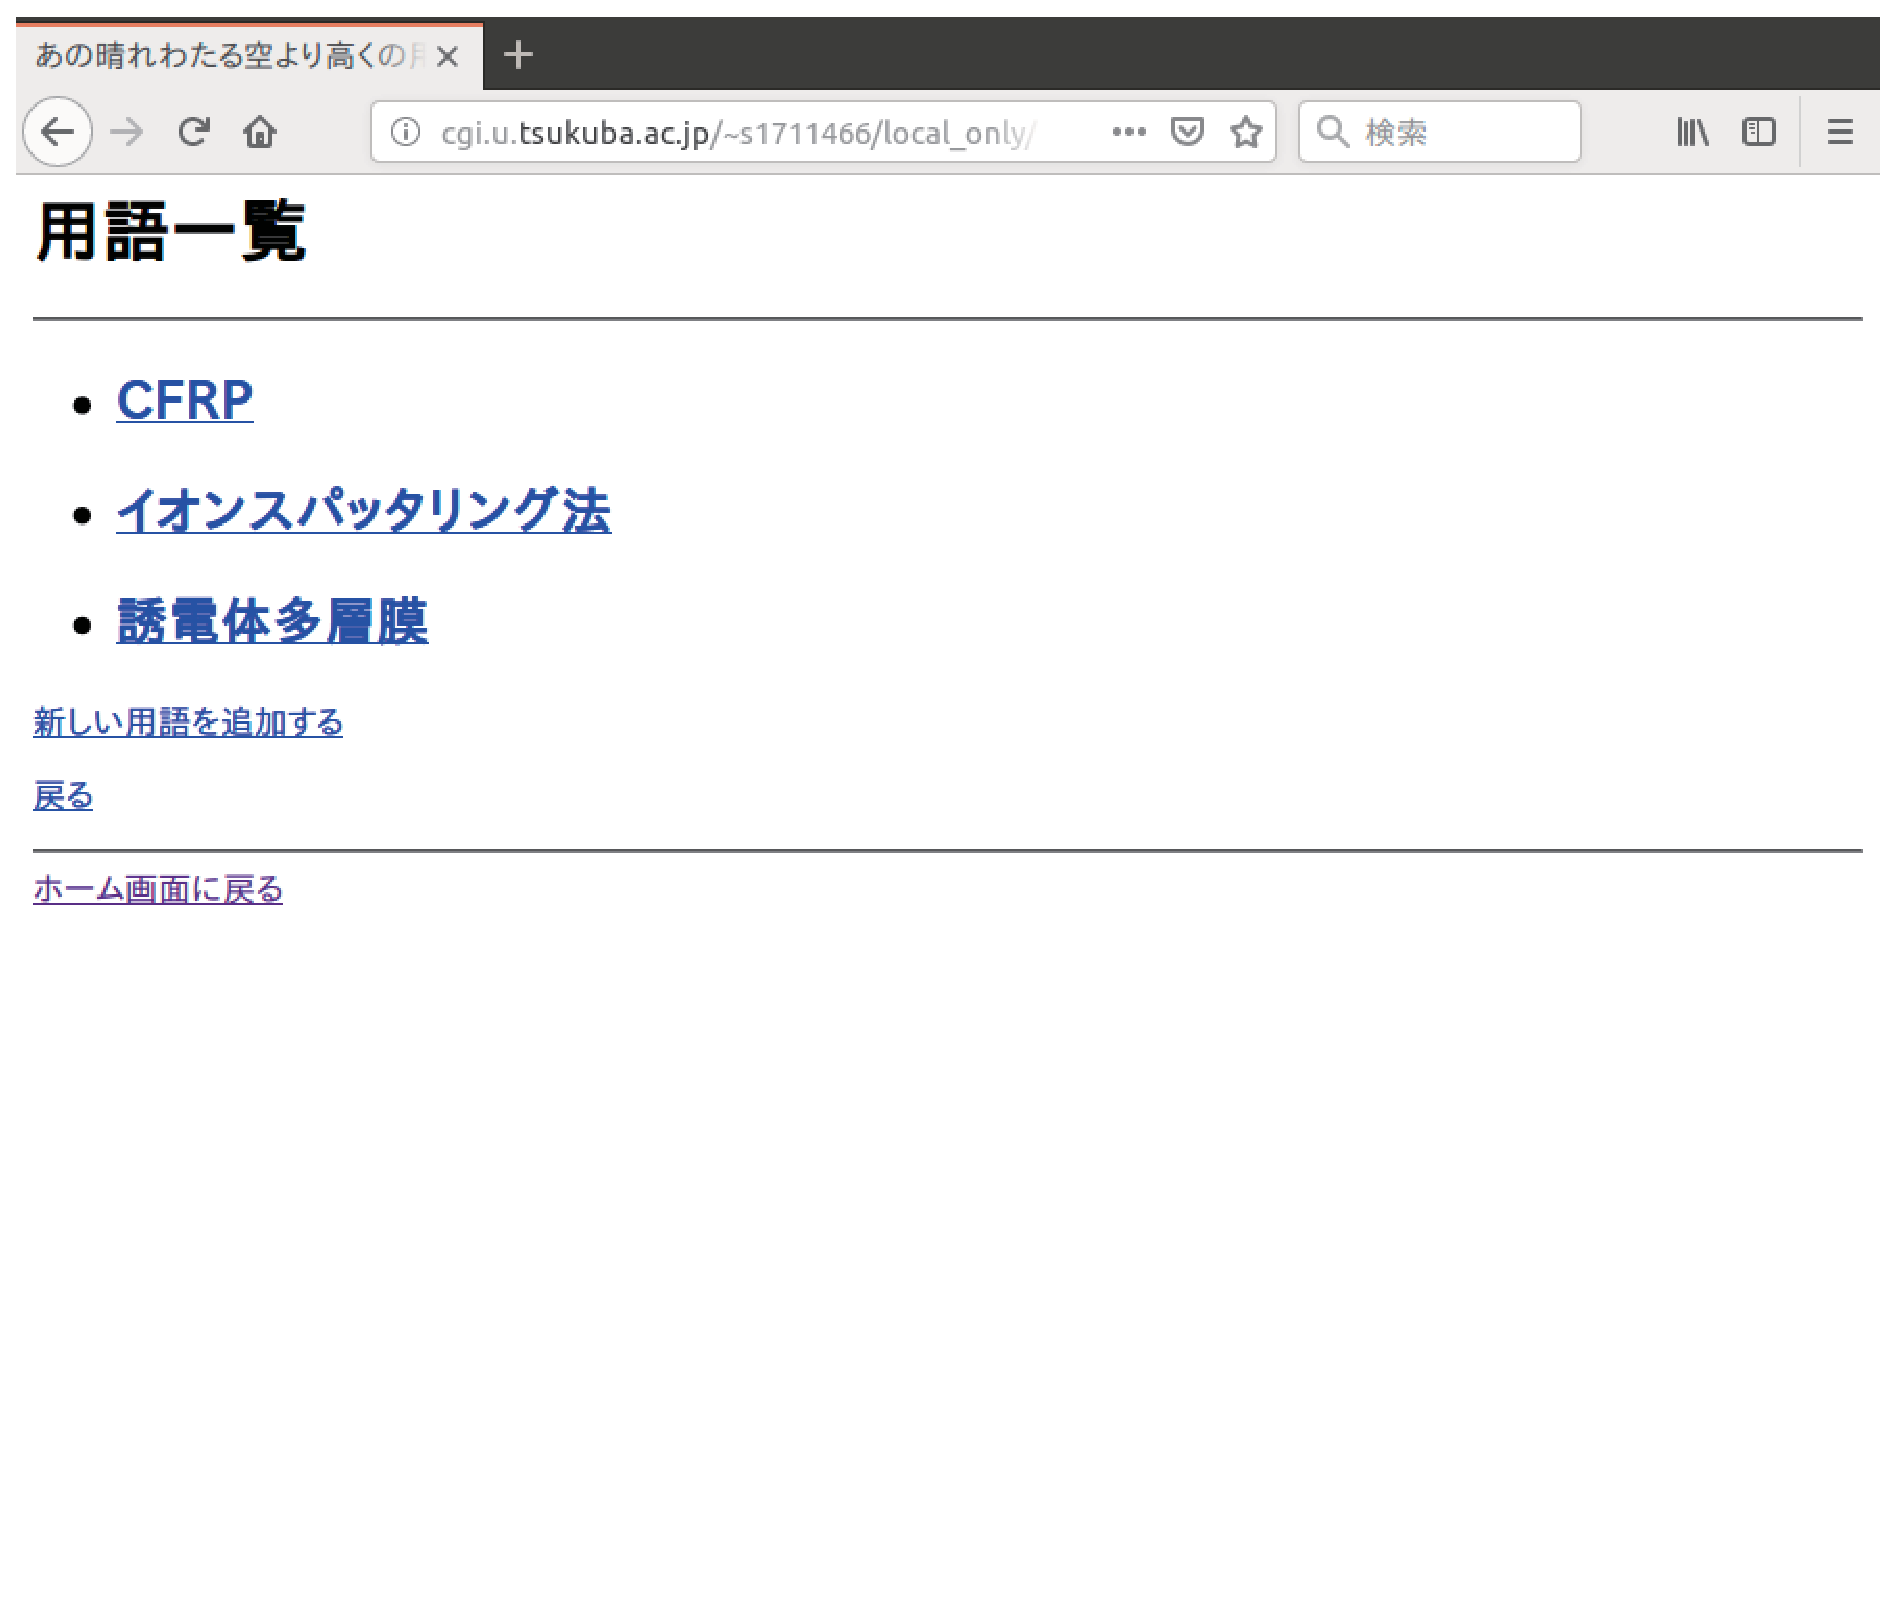
\includegraphics[width=6.7cm]{10-3-10.eps}
          \hspace{1.6cm} [4]新しい用語追加後の用語一覧
        \end{center}
      \end{minipage}

    \end{tabular}
    \caption{用語一覧及び追加関係の動作画面}
    \label{fig:b}
  \end{center}
\end{figure}

\begin{figure}[htbp]
  \begin{center}
    \begin{tabular}{c}

      % 1 ホーム画面
      \begin{minipage}{0.55\hsize}
        \begin{center}
          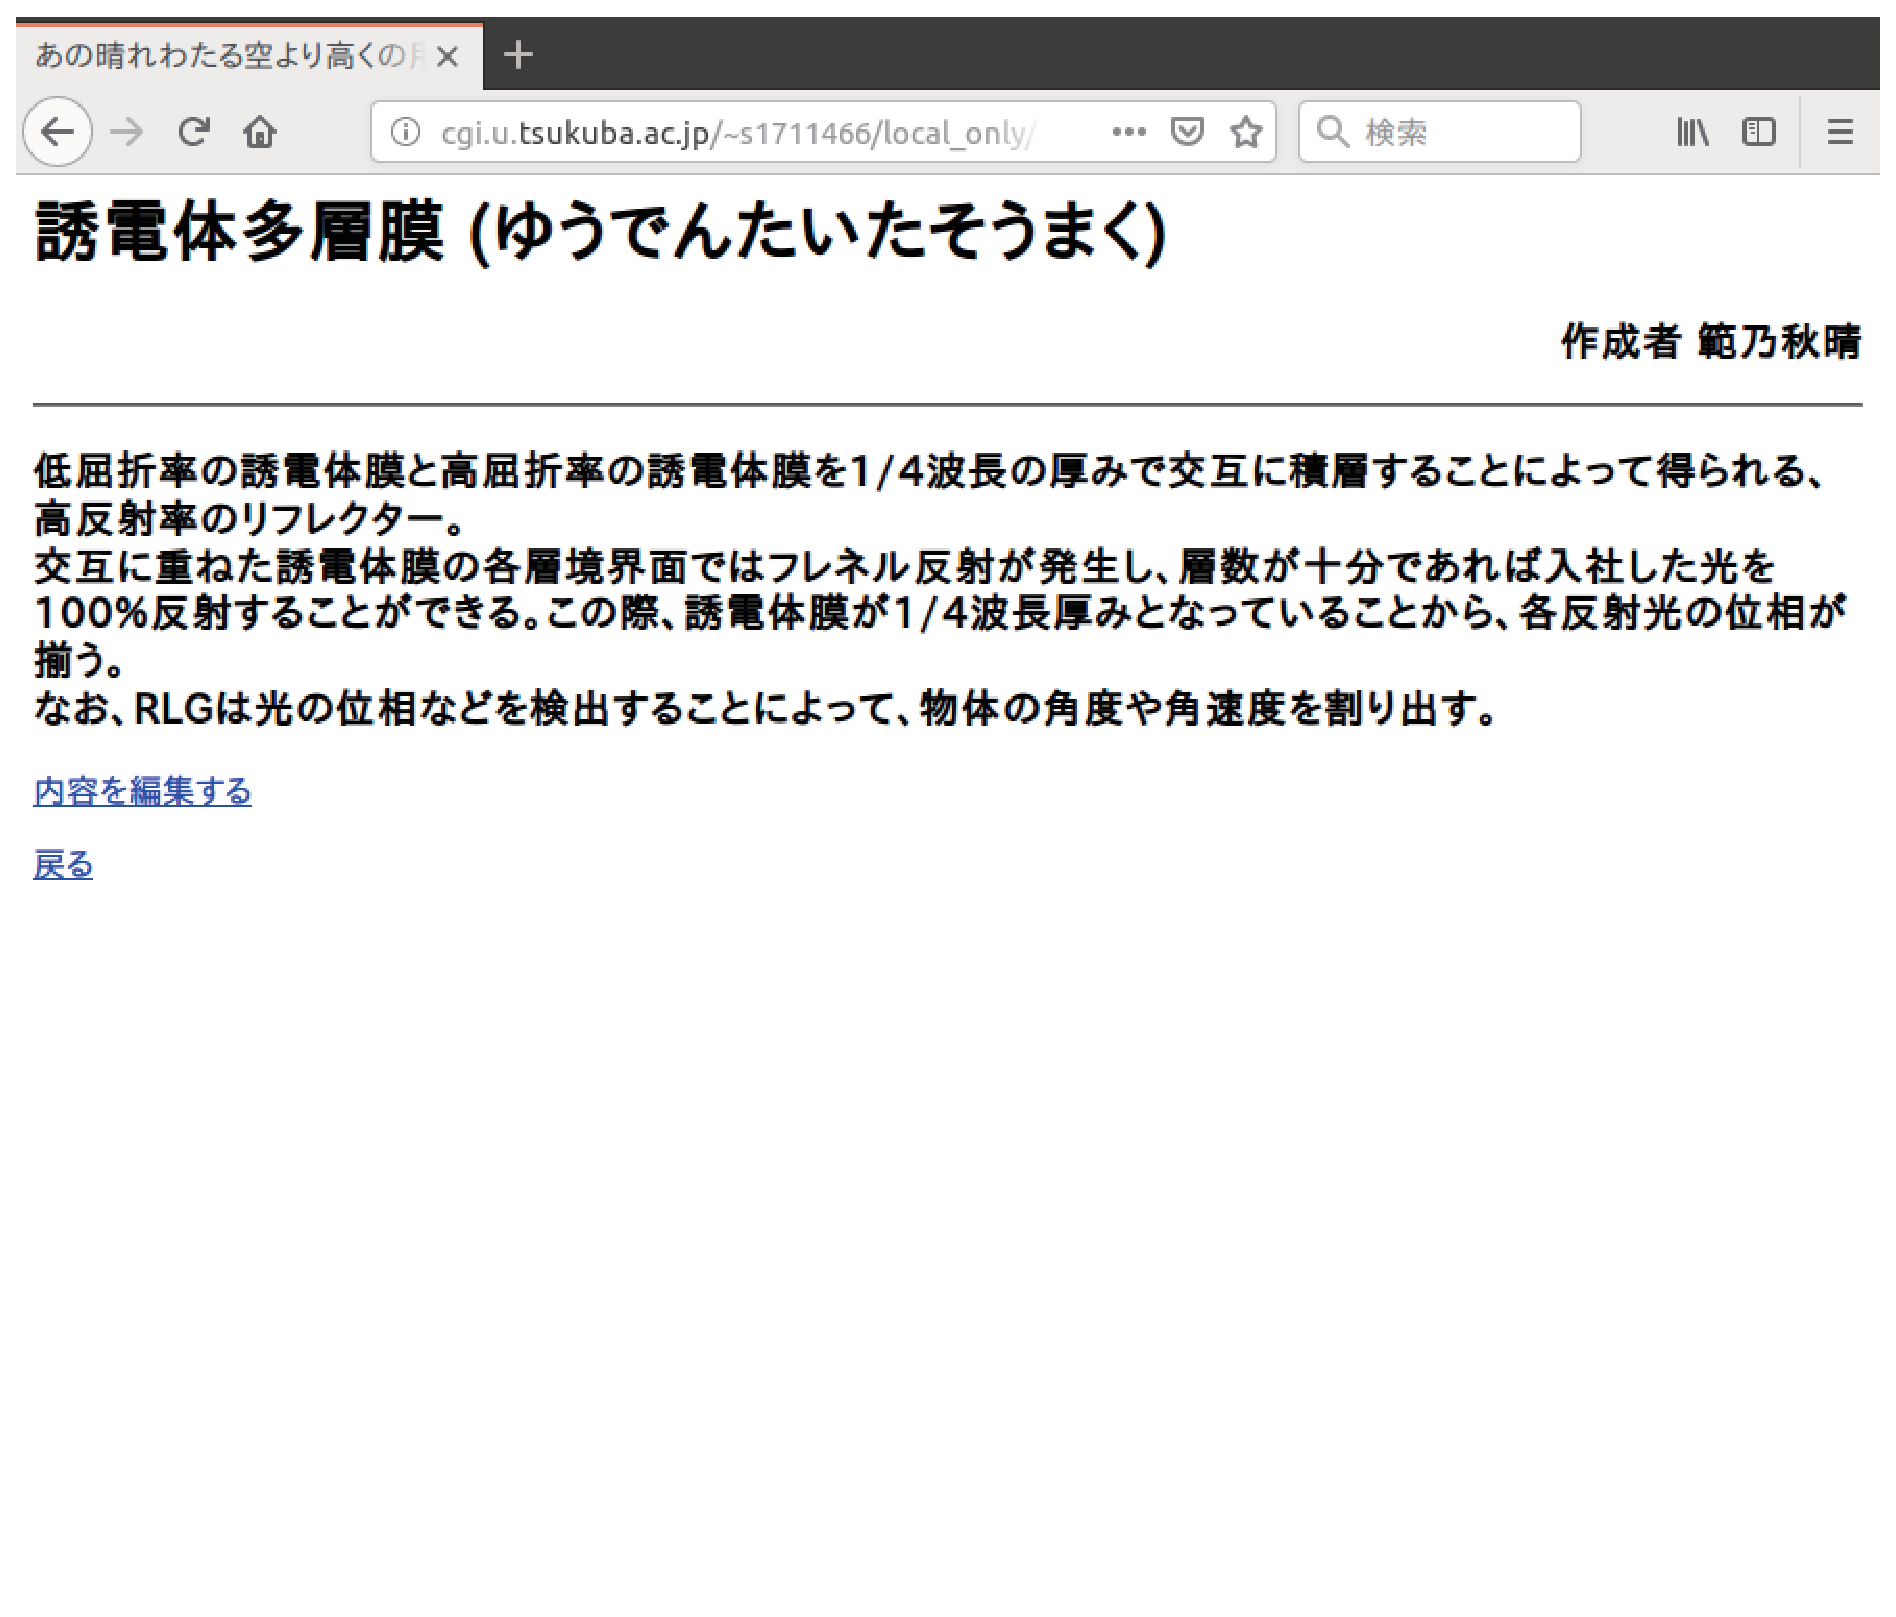
\includegraphics[width=7.0cm]{10-3-11.eps}
          \hspace{1.6cm} [1]用語の個別ページ
        \end{center}
      \end{minipage}

      % 2 
      \begin{minipage}{0.55\hsize}
        \begin{center}
          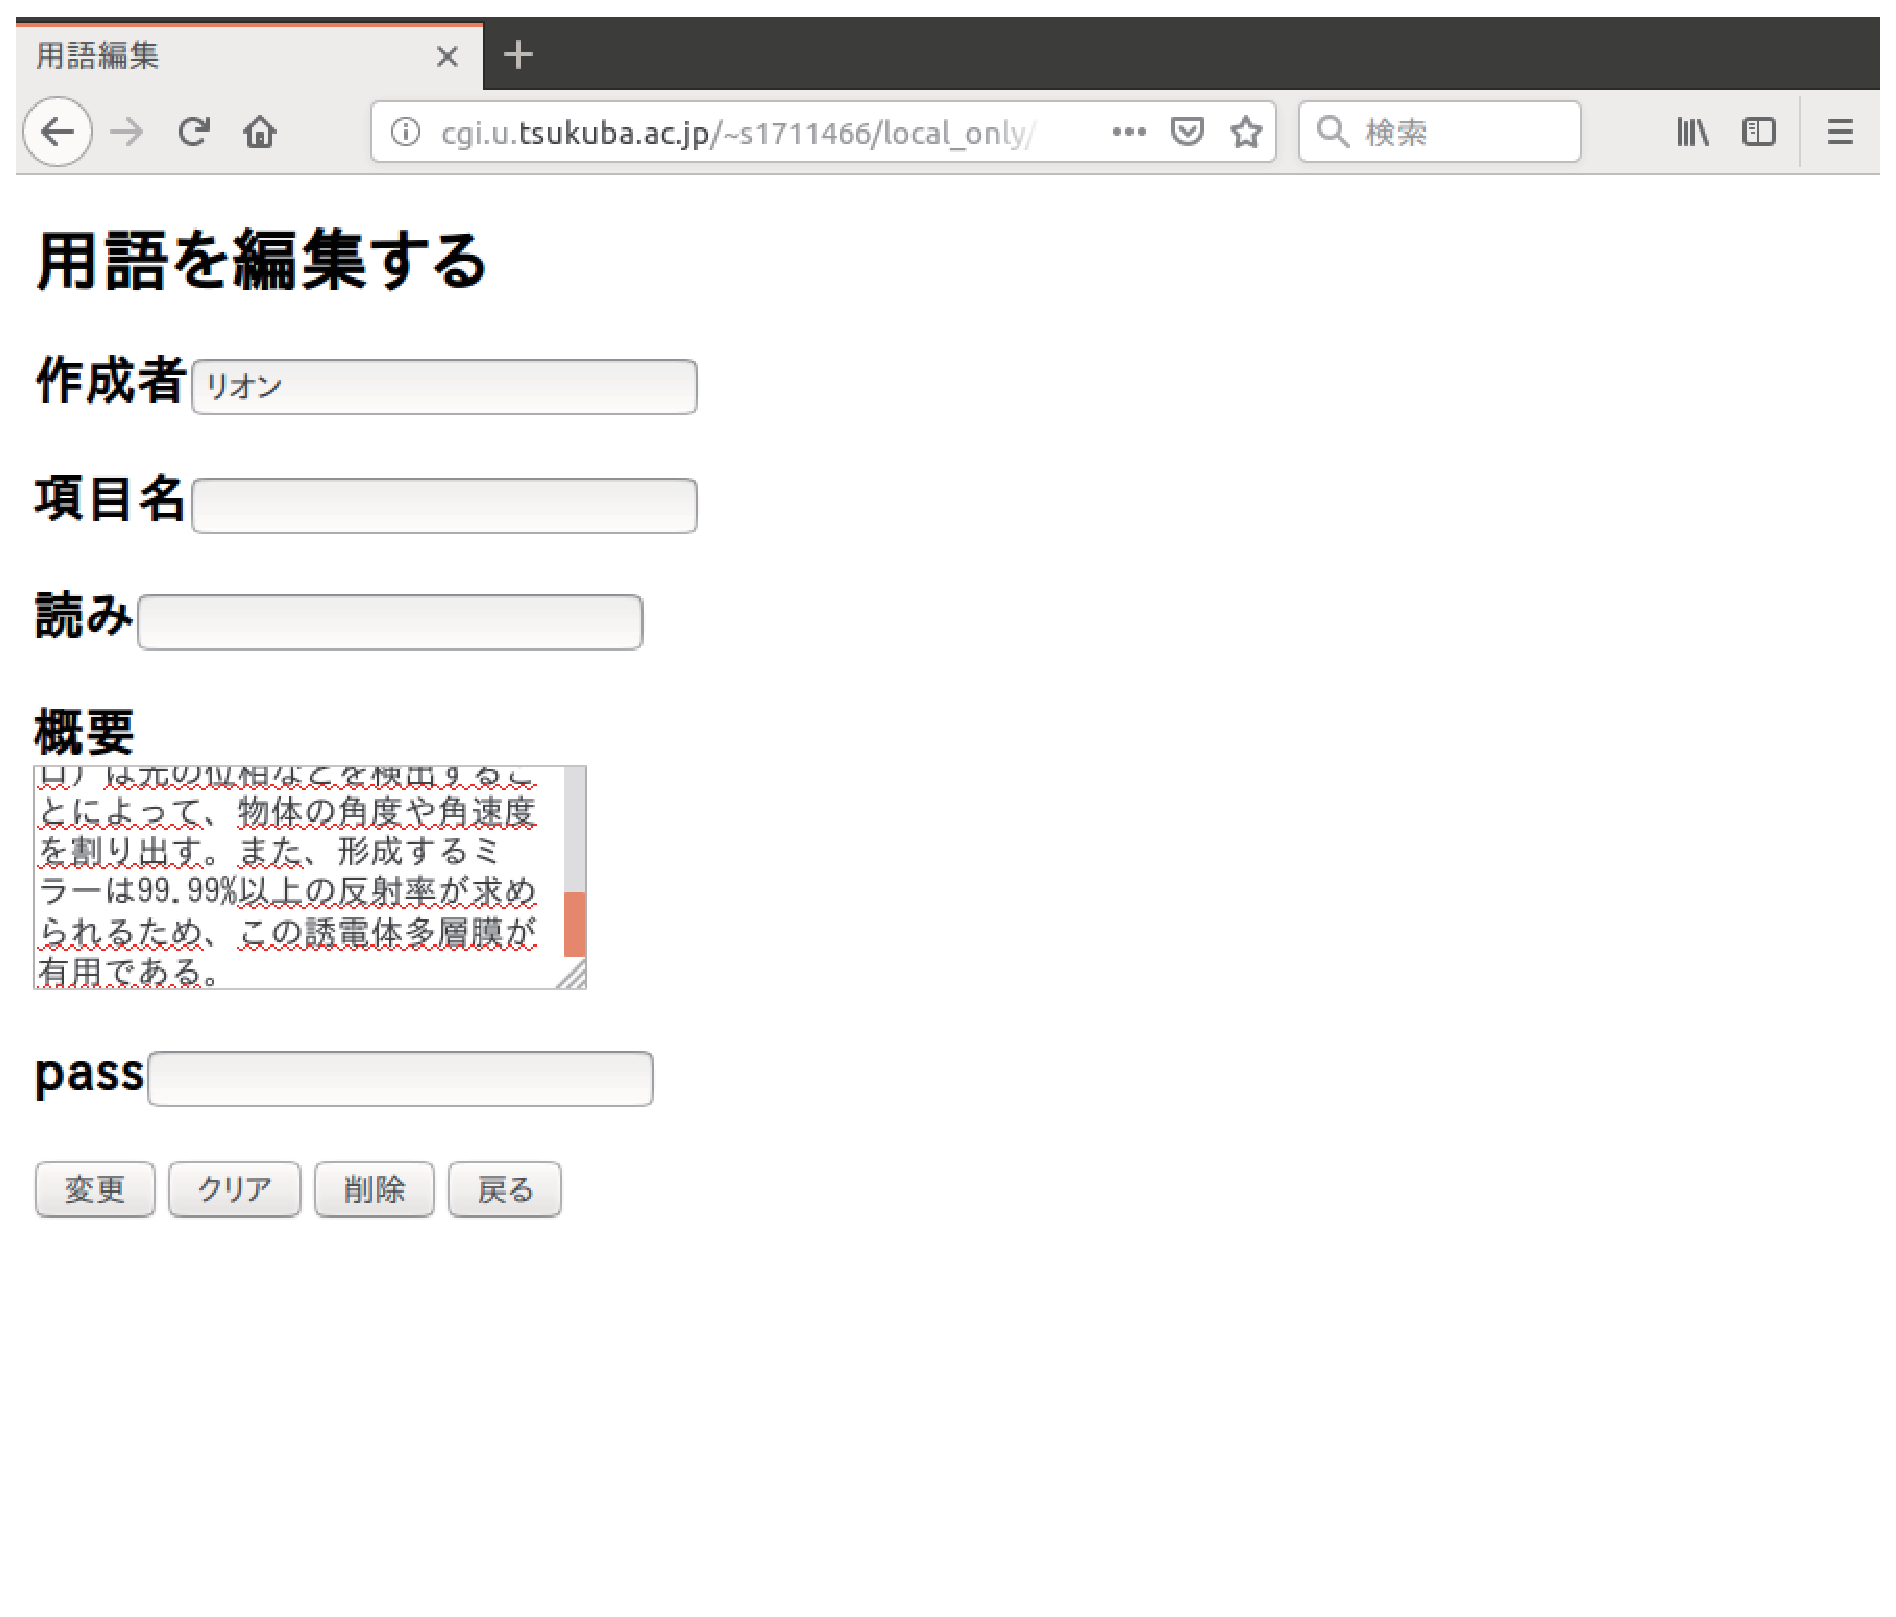
\includegraphics[width=6.7cm]{10-3-12.eps}
          \hspace{1.6cm} [2]用語の内容を編集する
        \end{center}
      \end{minipage}

      \begin{minipage}{0.55\hsize}
        \vspace{30mm}
      \end{minipage} \\
 
      % 3
      \begin{minipage}{0.5\hsize}
        \begin{center}
          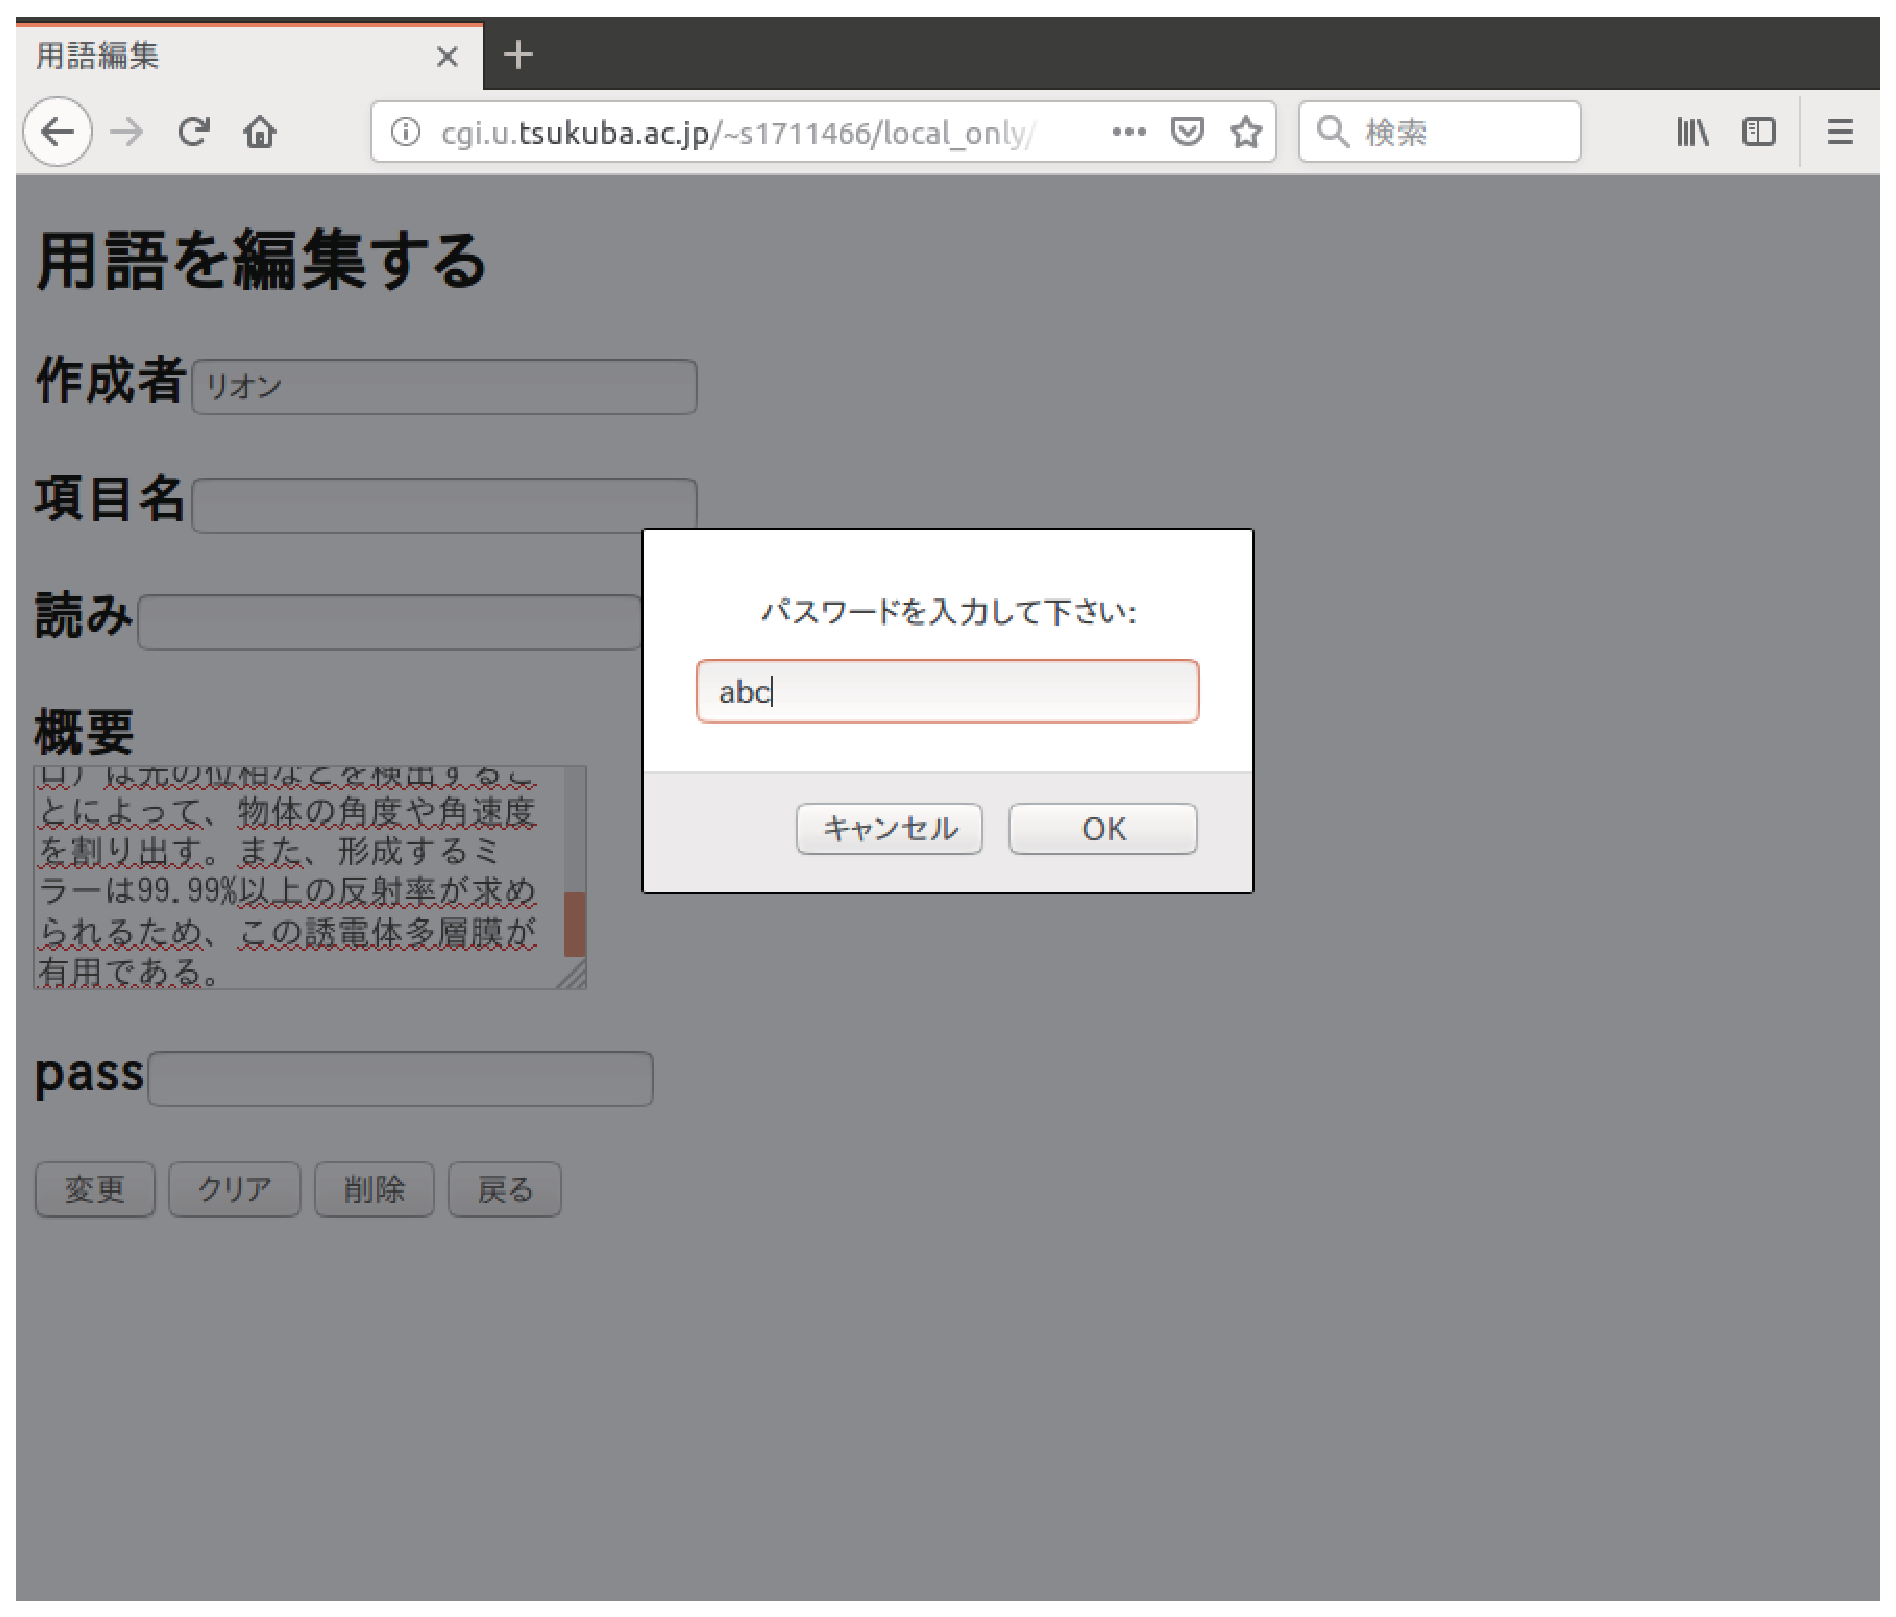
\includegraphics[width=6.7cm]{10-3-13.eps}
          \hspace{1.6cm} [3]パスワード要求
        \end{center}
      \end{minipage}

      % 4
      \begin{minipage}{0.55\hsize}
        \begin{center}
          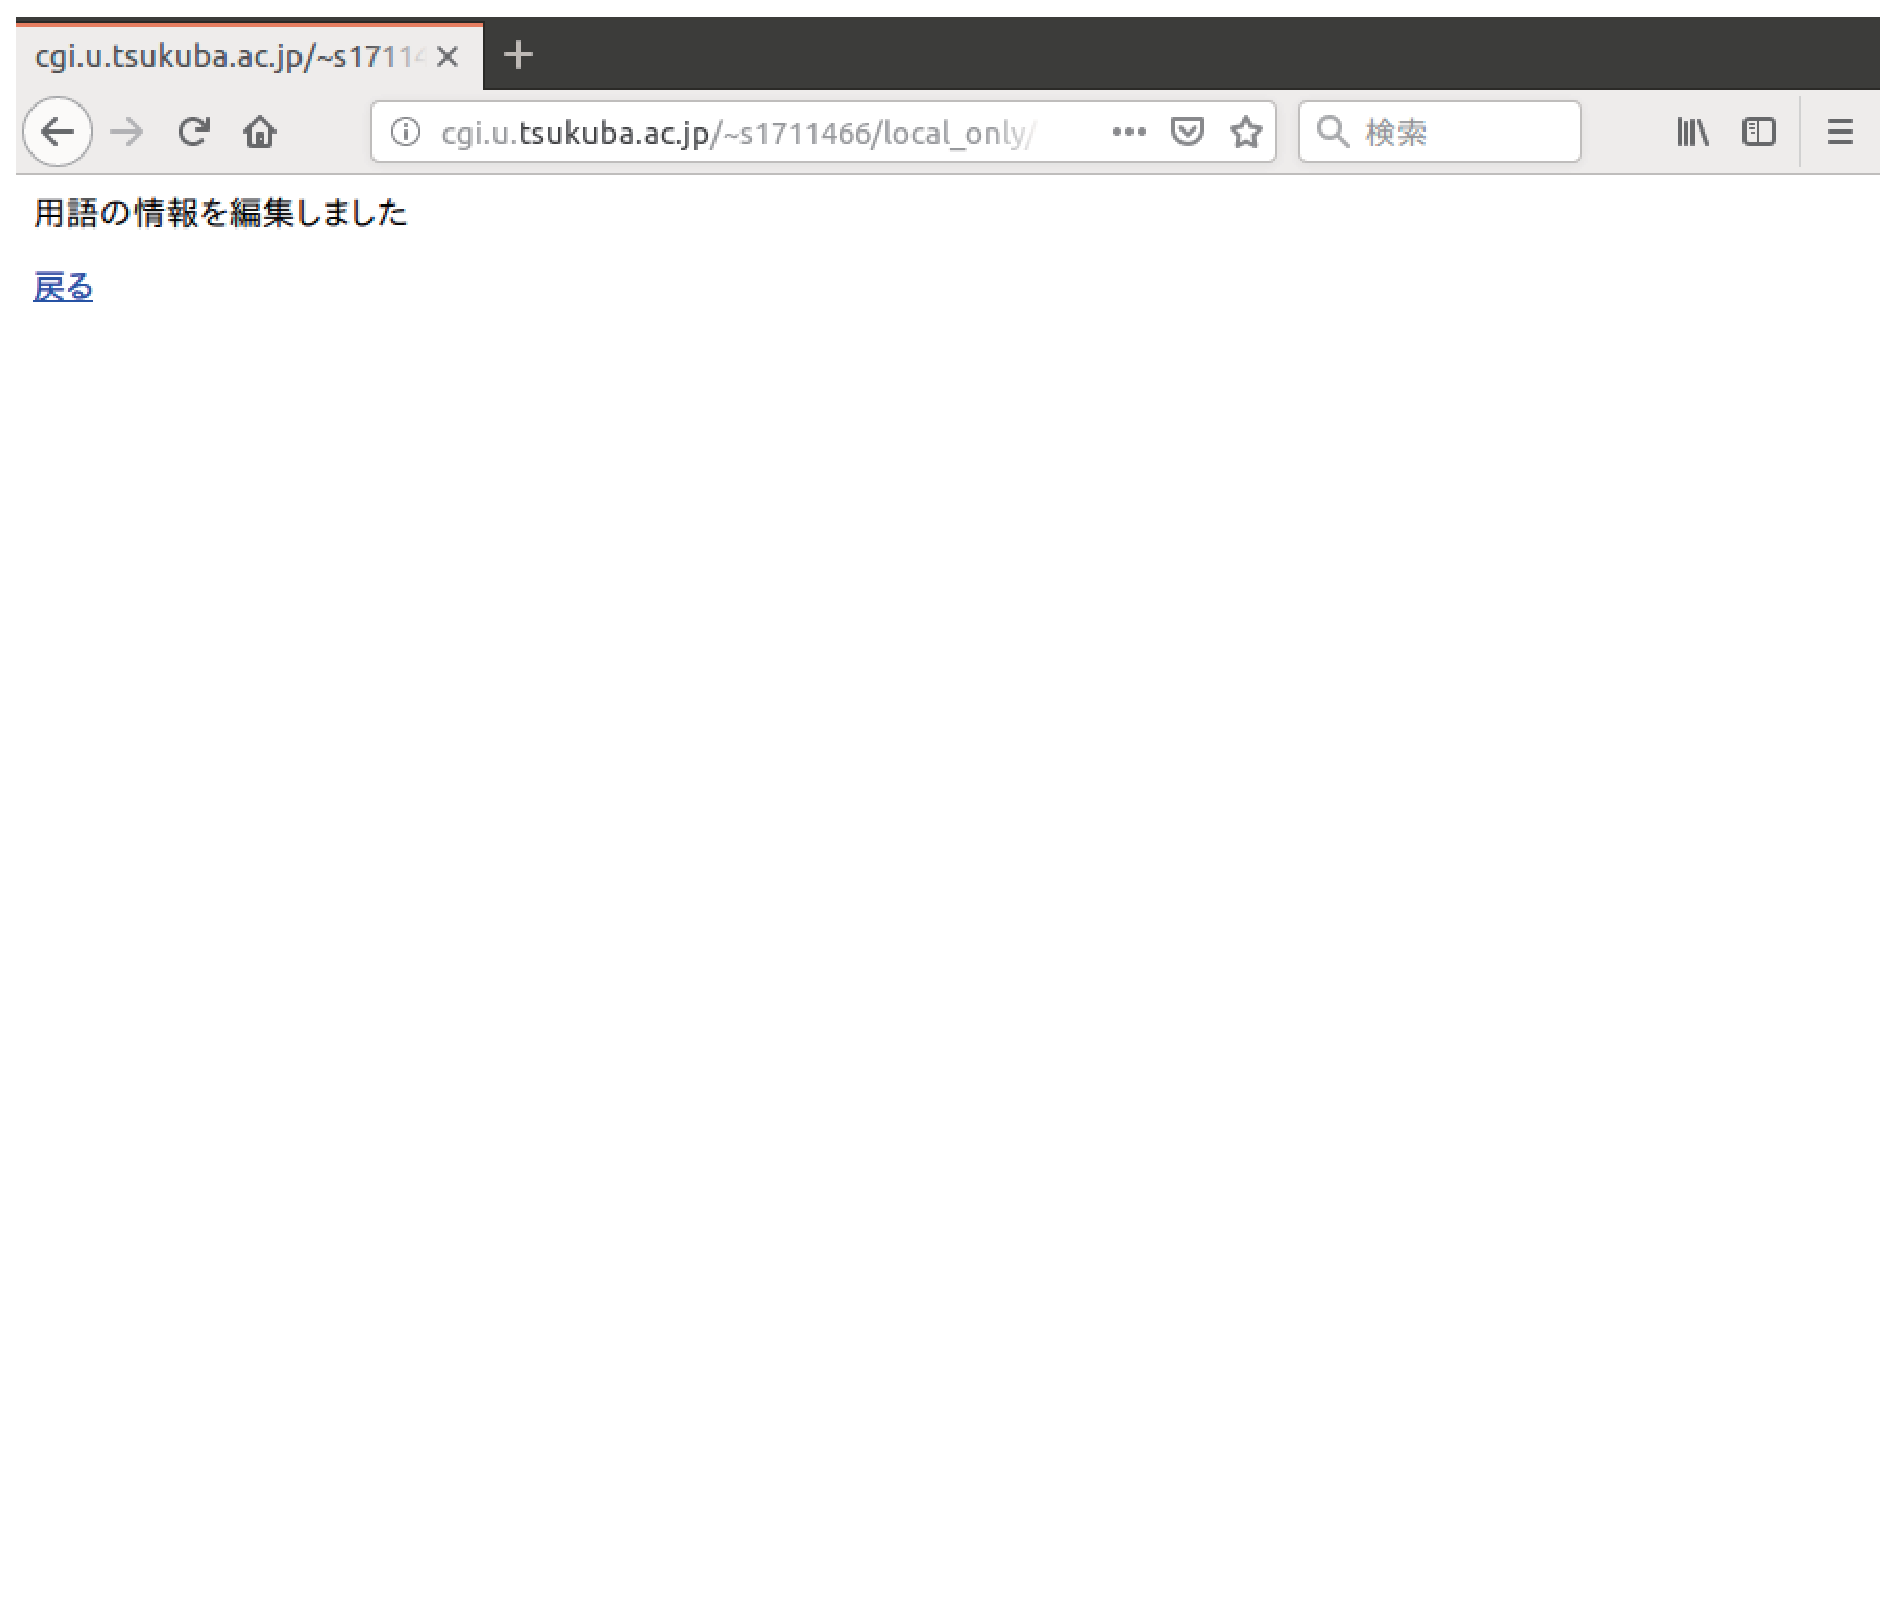
\includegraphics[width=6.7cm]{10-3-14.eps}
          \hspace{1.6cm} [4]編集完了
        \end{center}
      \end{minipage}

      \begin{minipage}{0.55\hsize}
        \vspace{90mm}
      \end{minipage} \\

      % 5
      \begin{minipage}{0.55\hsize}
        \begin{center}
          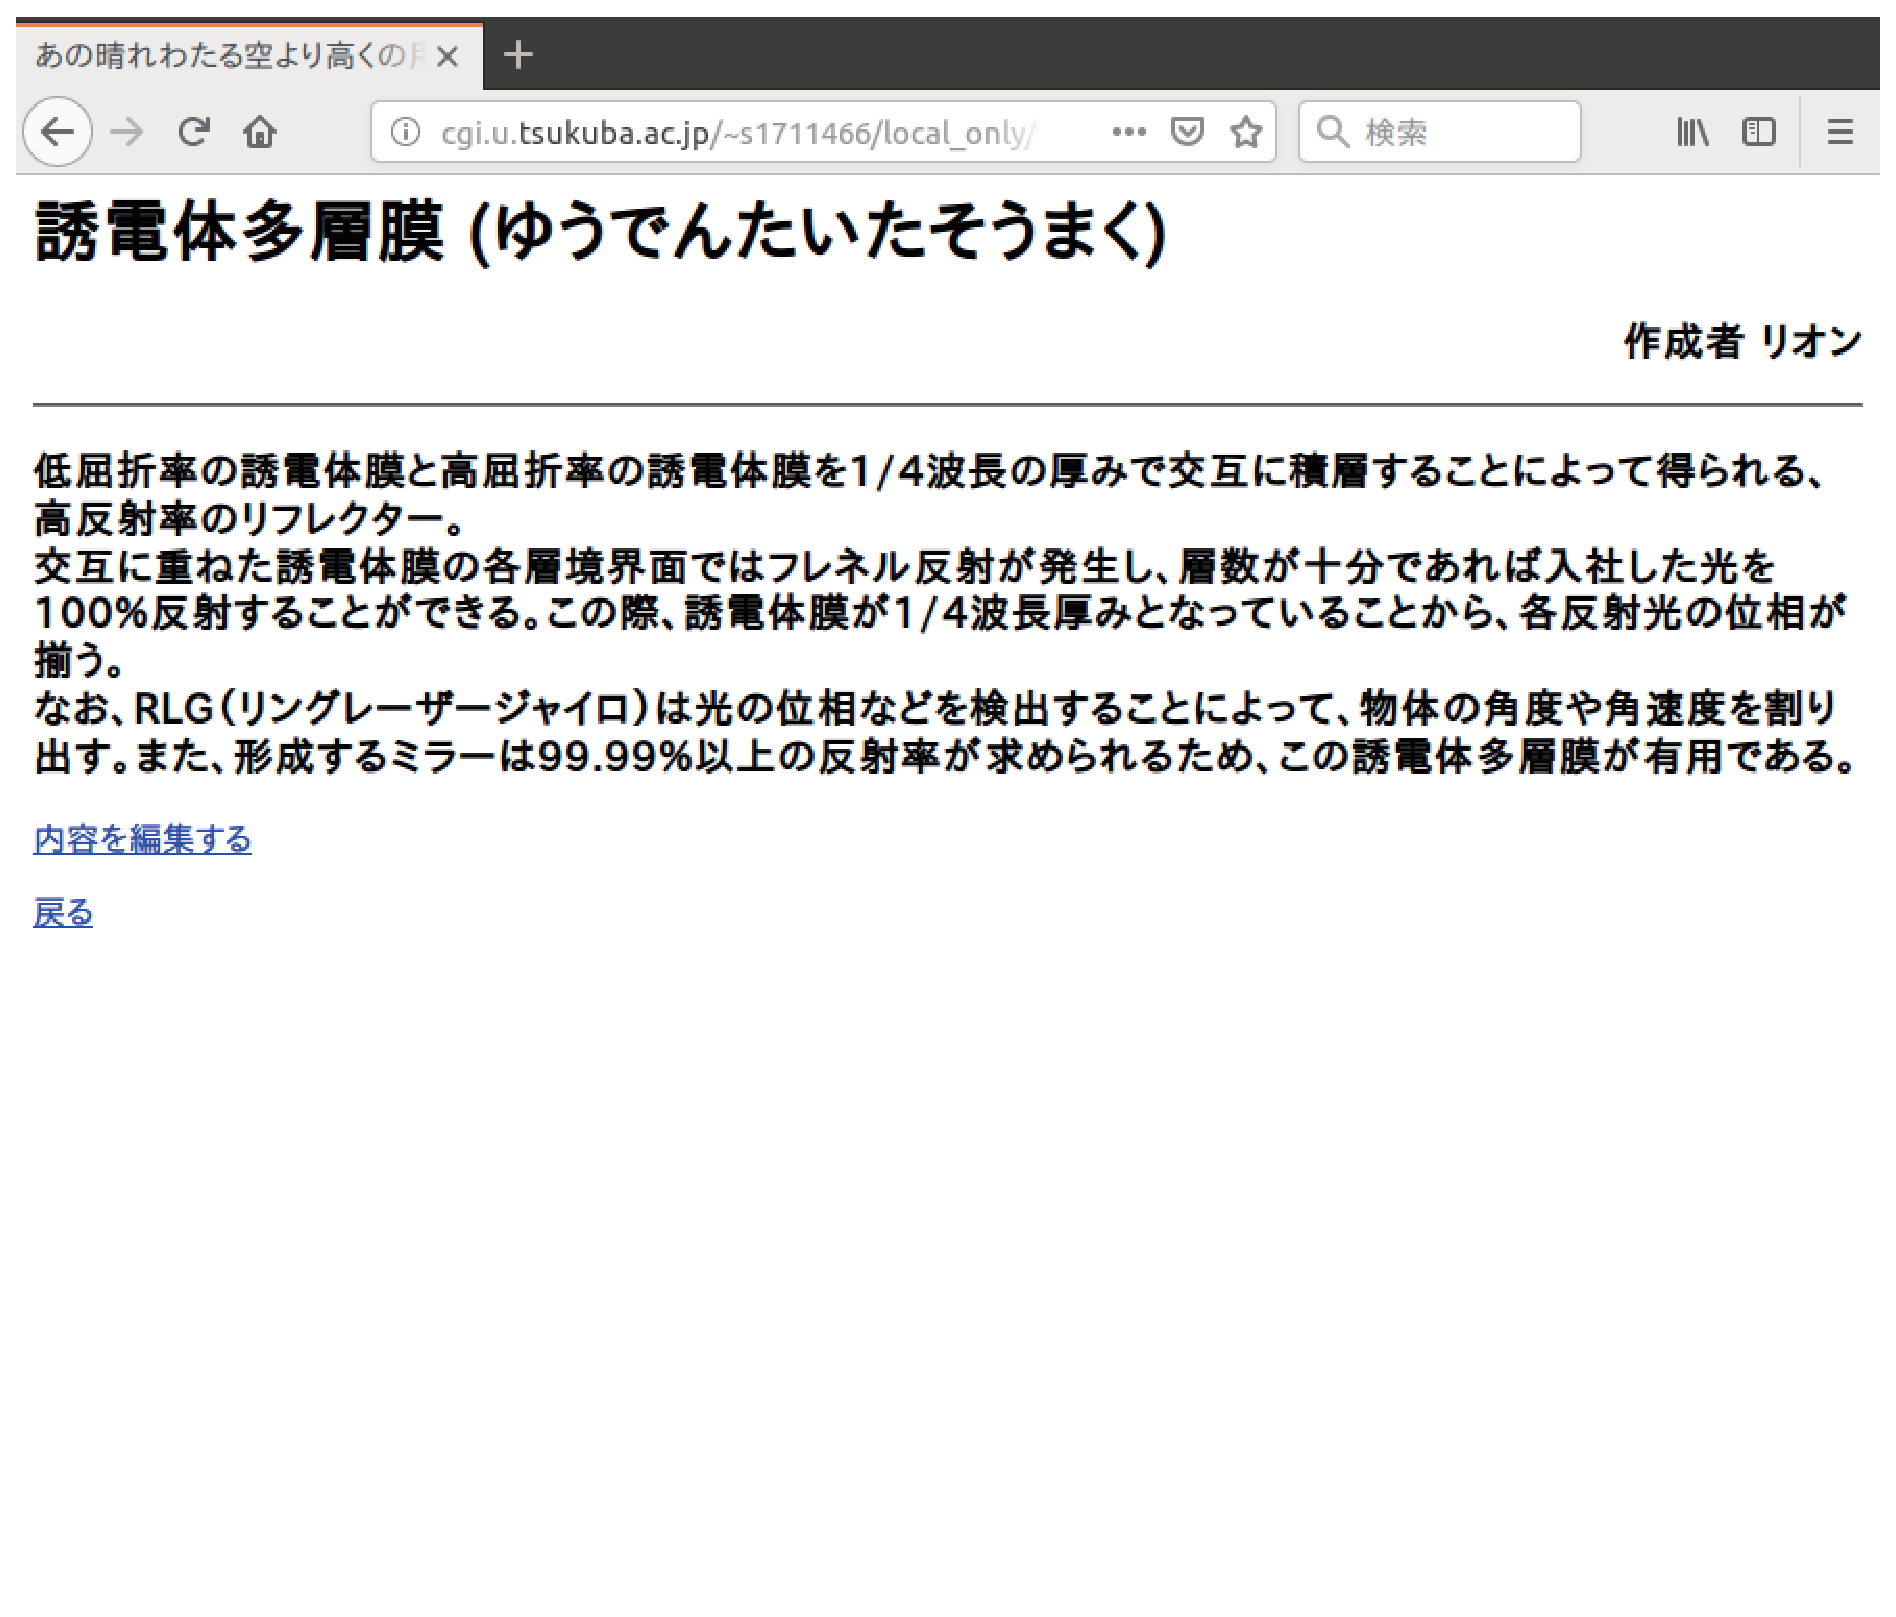
\includegraphics[width=6.7cm]{10-3-15.eps}
          \hspace{1.6cm} [5]内容編集後の用語の個別ページ
        \end{center}
      \end{minipage}

    \end{tabular}
    \caption{用語の編集関係の動作画面}
    \label{fig:b}
  \end{center}
\end{figure}

\begin{figure}[htbp]
  \begin{center}
    \begin{tabular}{c}

      % 1 ホーム画面
      \begin{minipage}{0.55\hsize}
        \begin{center}
          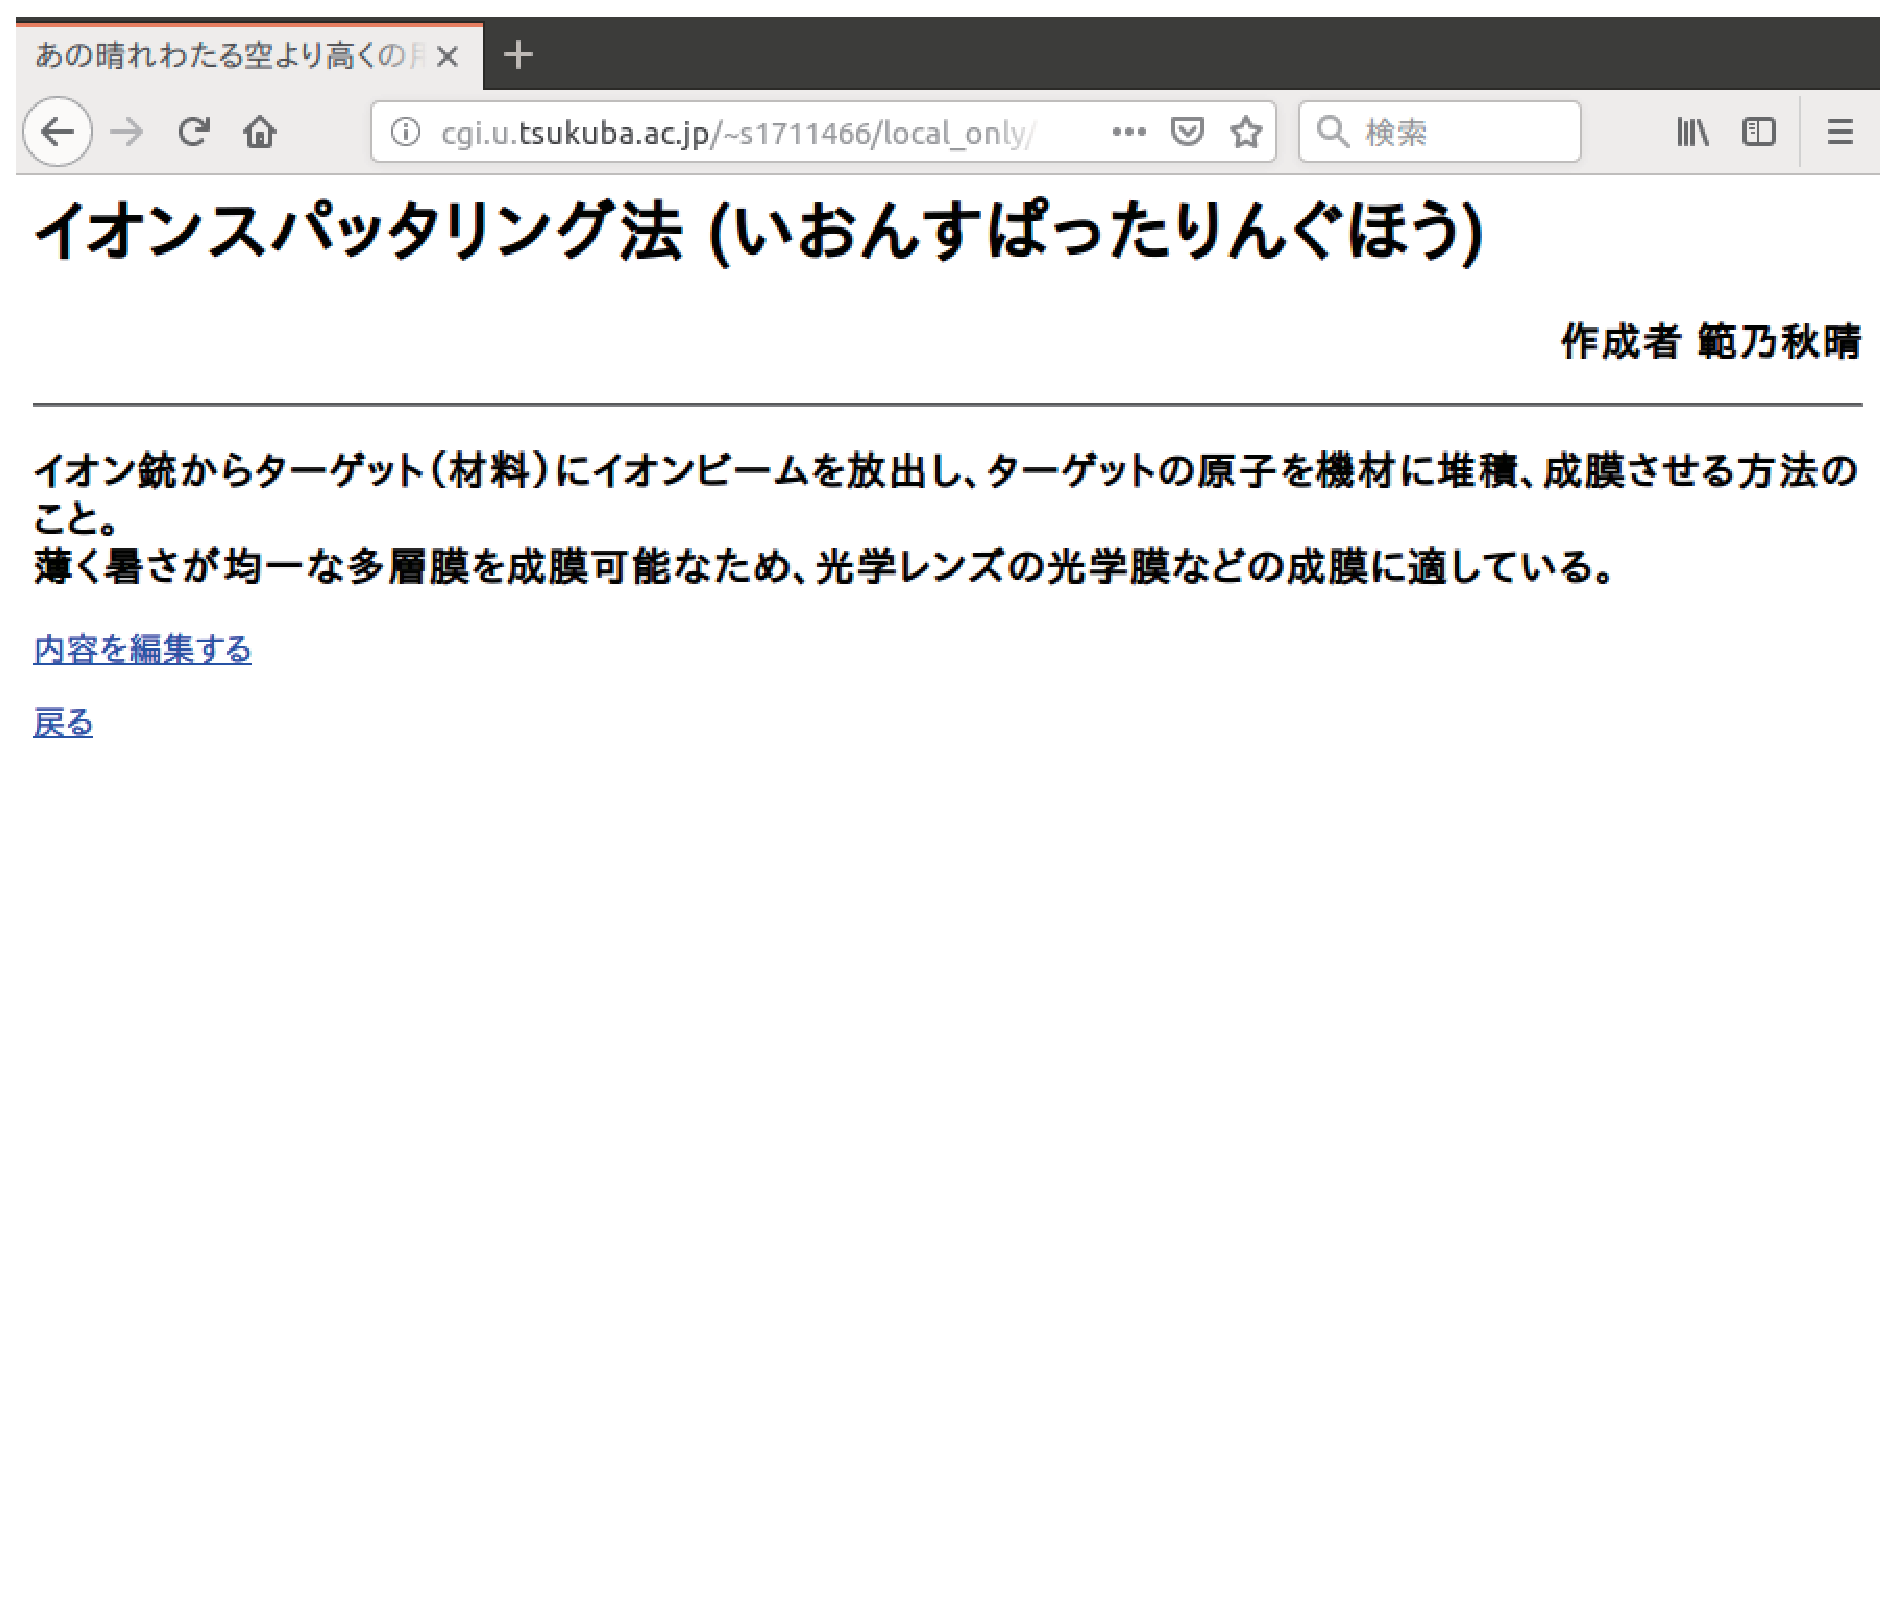
\includegraphics[width=7.0cm]{10-3-16.eps}
          \hspace{1.6cm} [1]用語の個別ページ
        \end{center}
      \end{minipage}

      % 2 
      \begin{minipage}{0.55\hsize}
        \begin{center}
          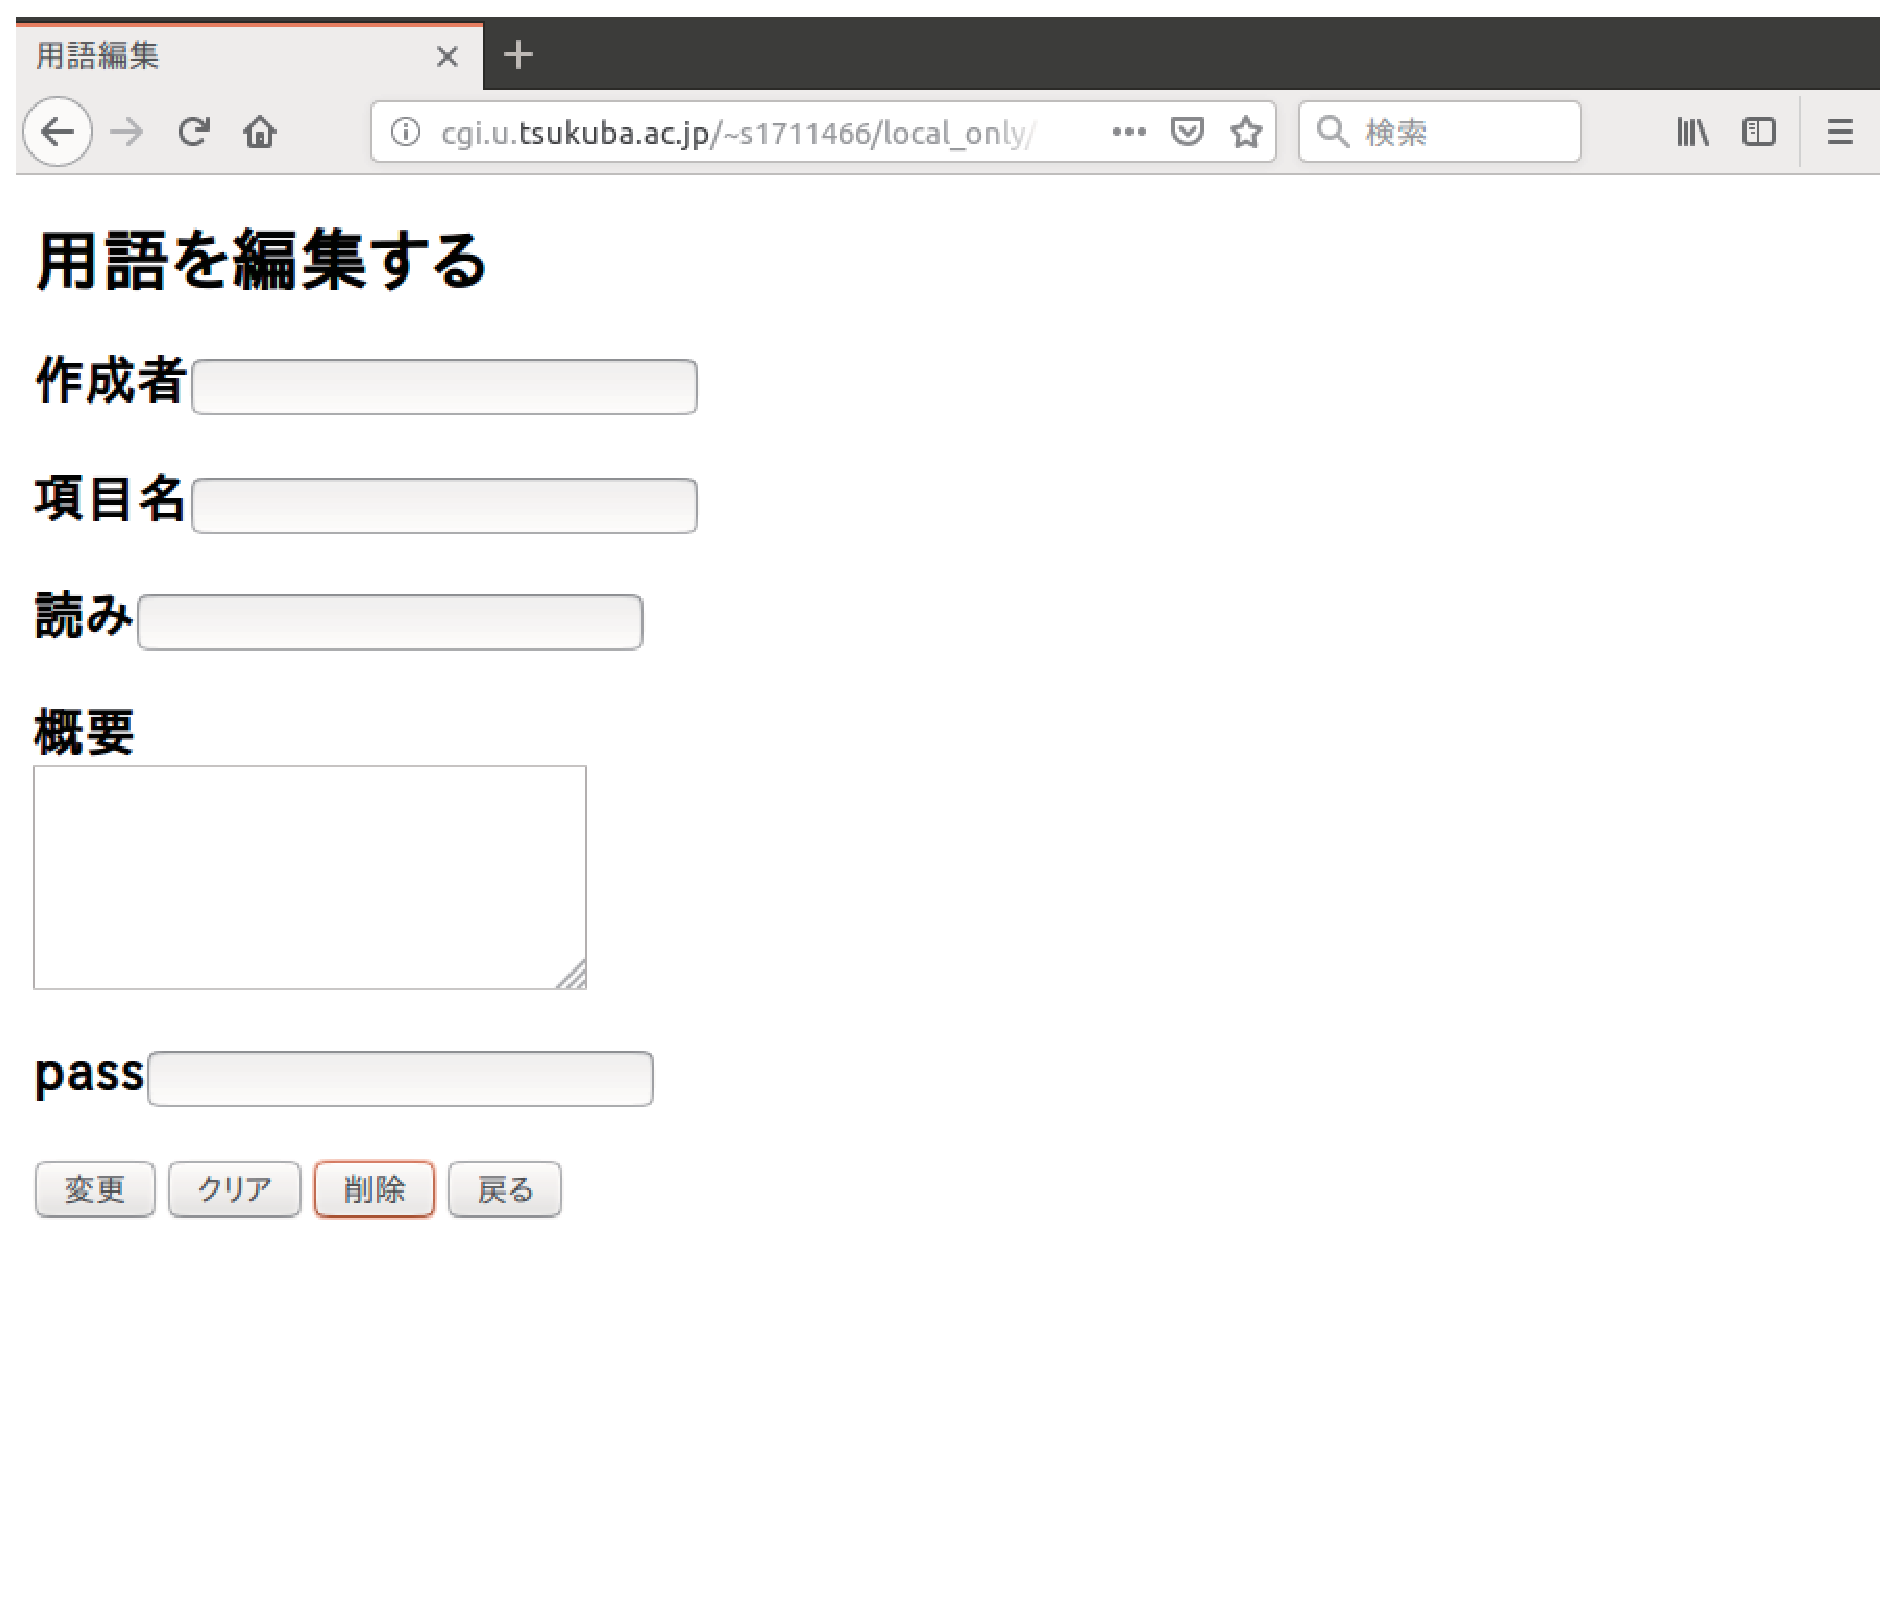
\includegraphics[width=6.7cm]{10-3-17.eps}
          \hspace{1.6cm} [2]用語を削除する
        \end{center}
      \end{minipage}

      \begin{minipage}{0.55\hsize}
        \vspace{30mm}
      \end{minipage} \\
 
      % 3
      \begin{minipage}{0.5\hsize}
        \begin{center}
          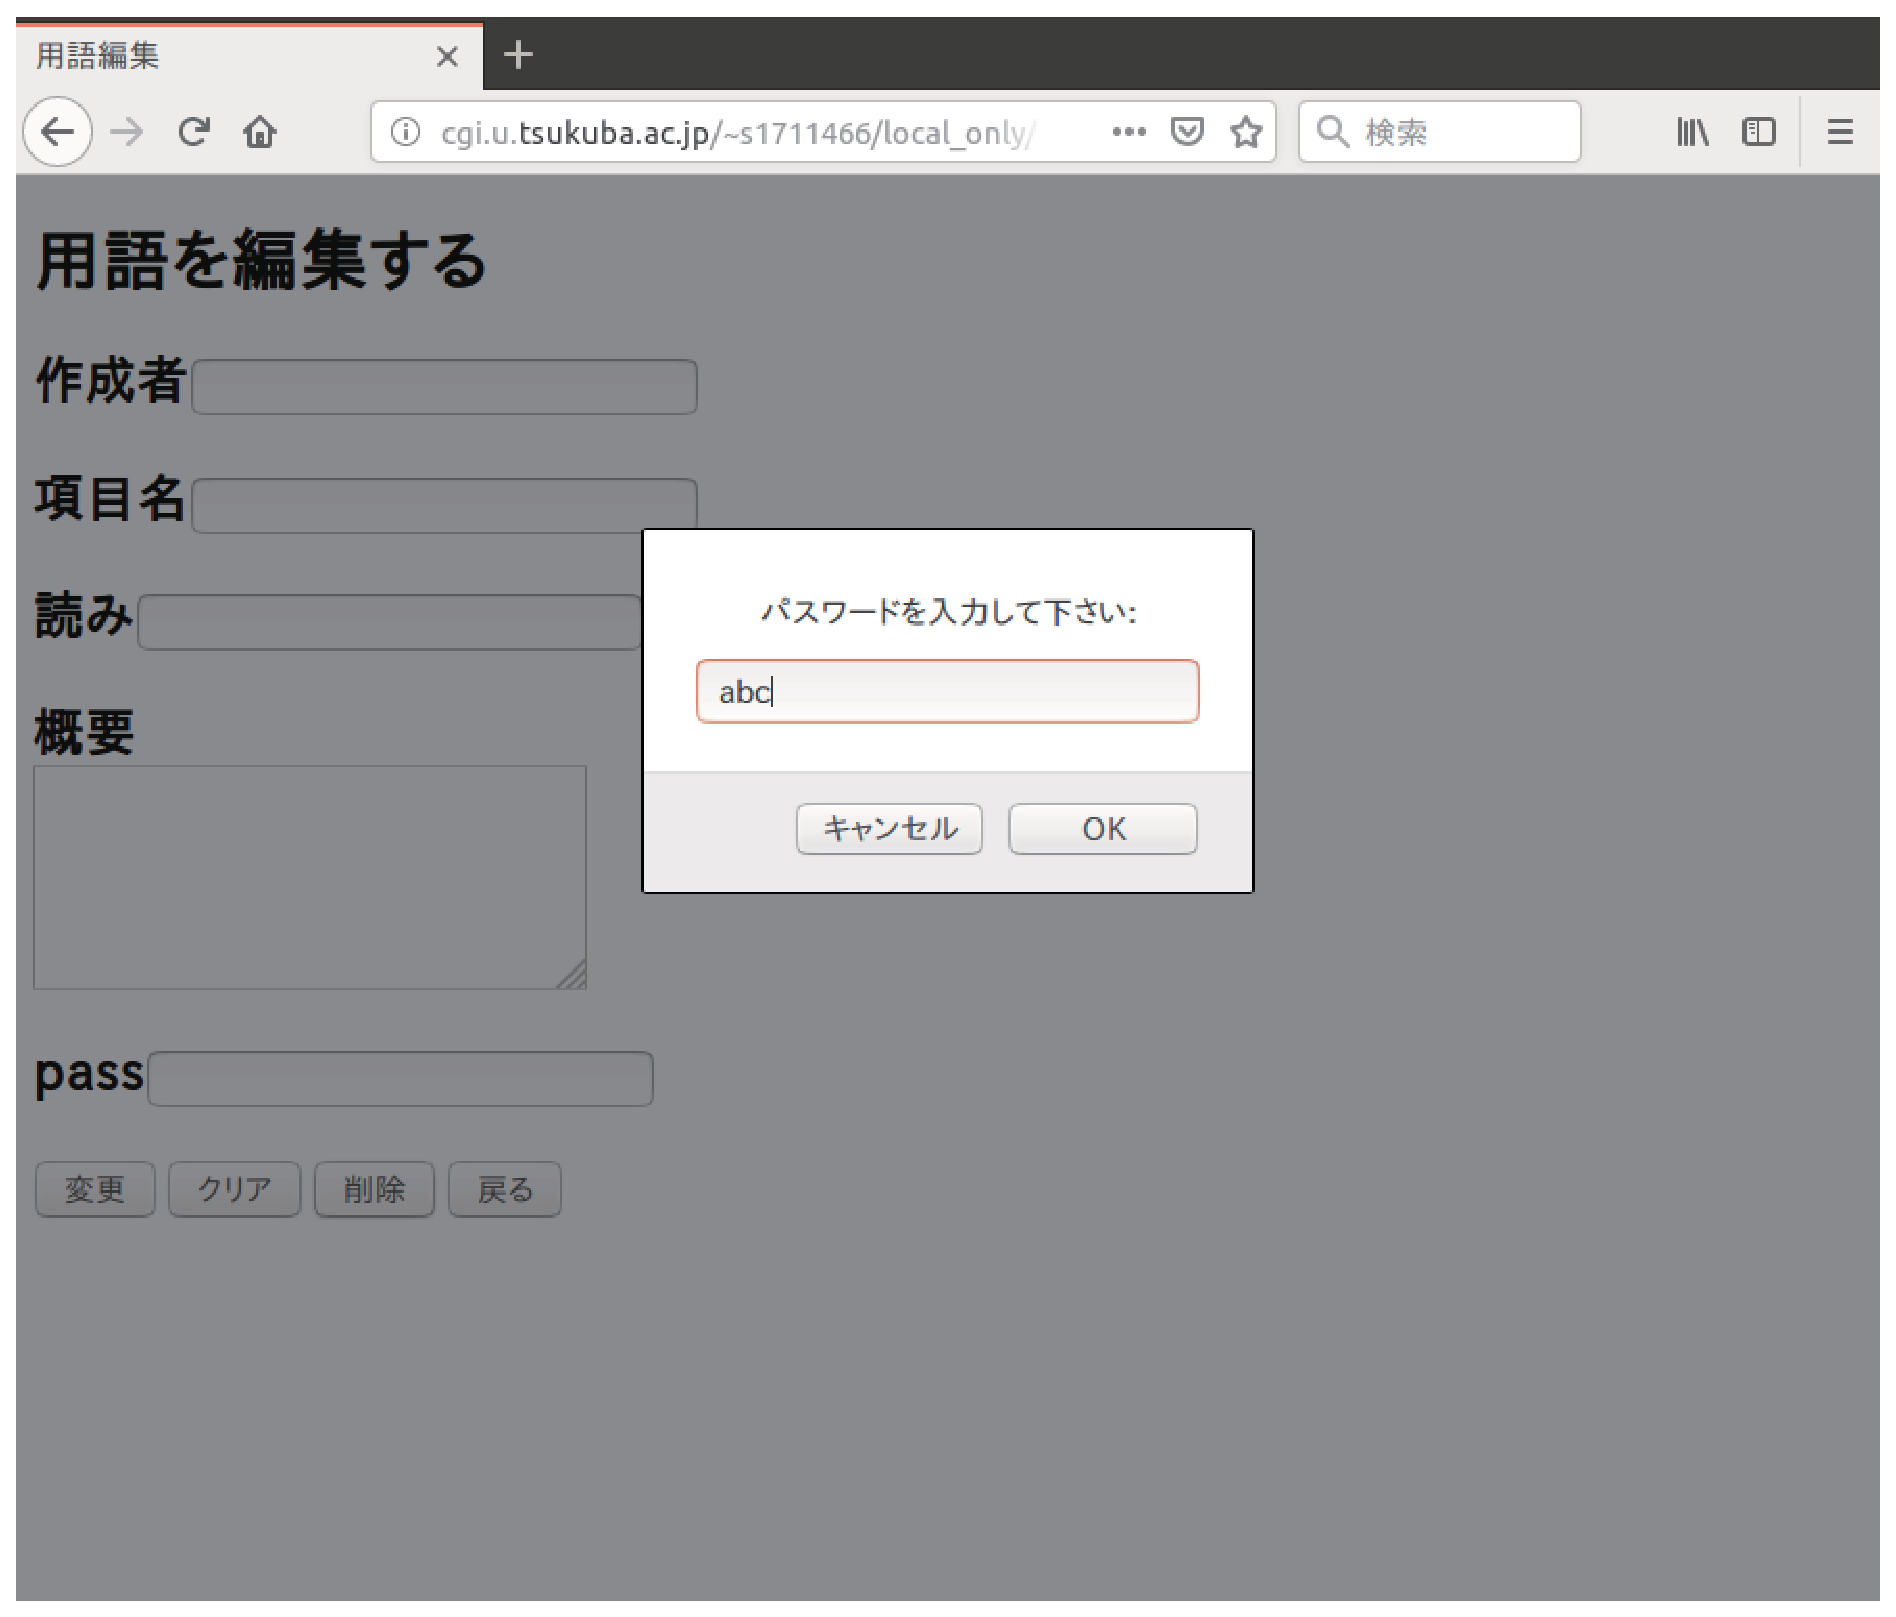
\includegraphics[width=6.7cm]{10-3-18.eps}
          \hspace{1.6cm} [3]パスワード要求
        \end{center}
      \end{minipage}

      % 4
      \begin{minipage}{0.55\hsize}
        \begin{center}
          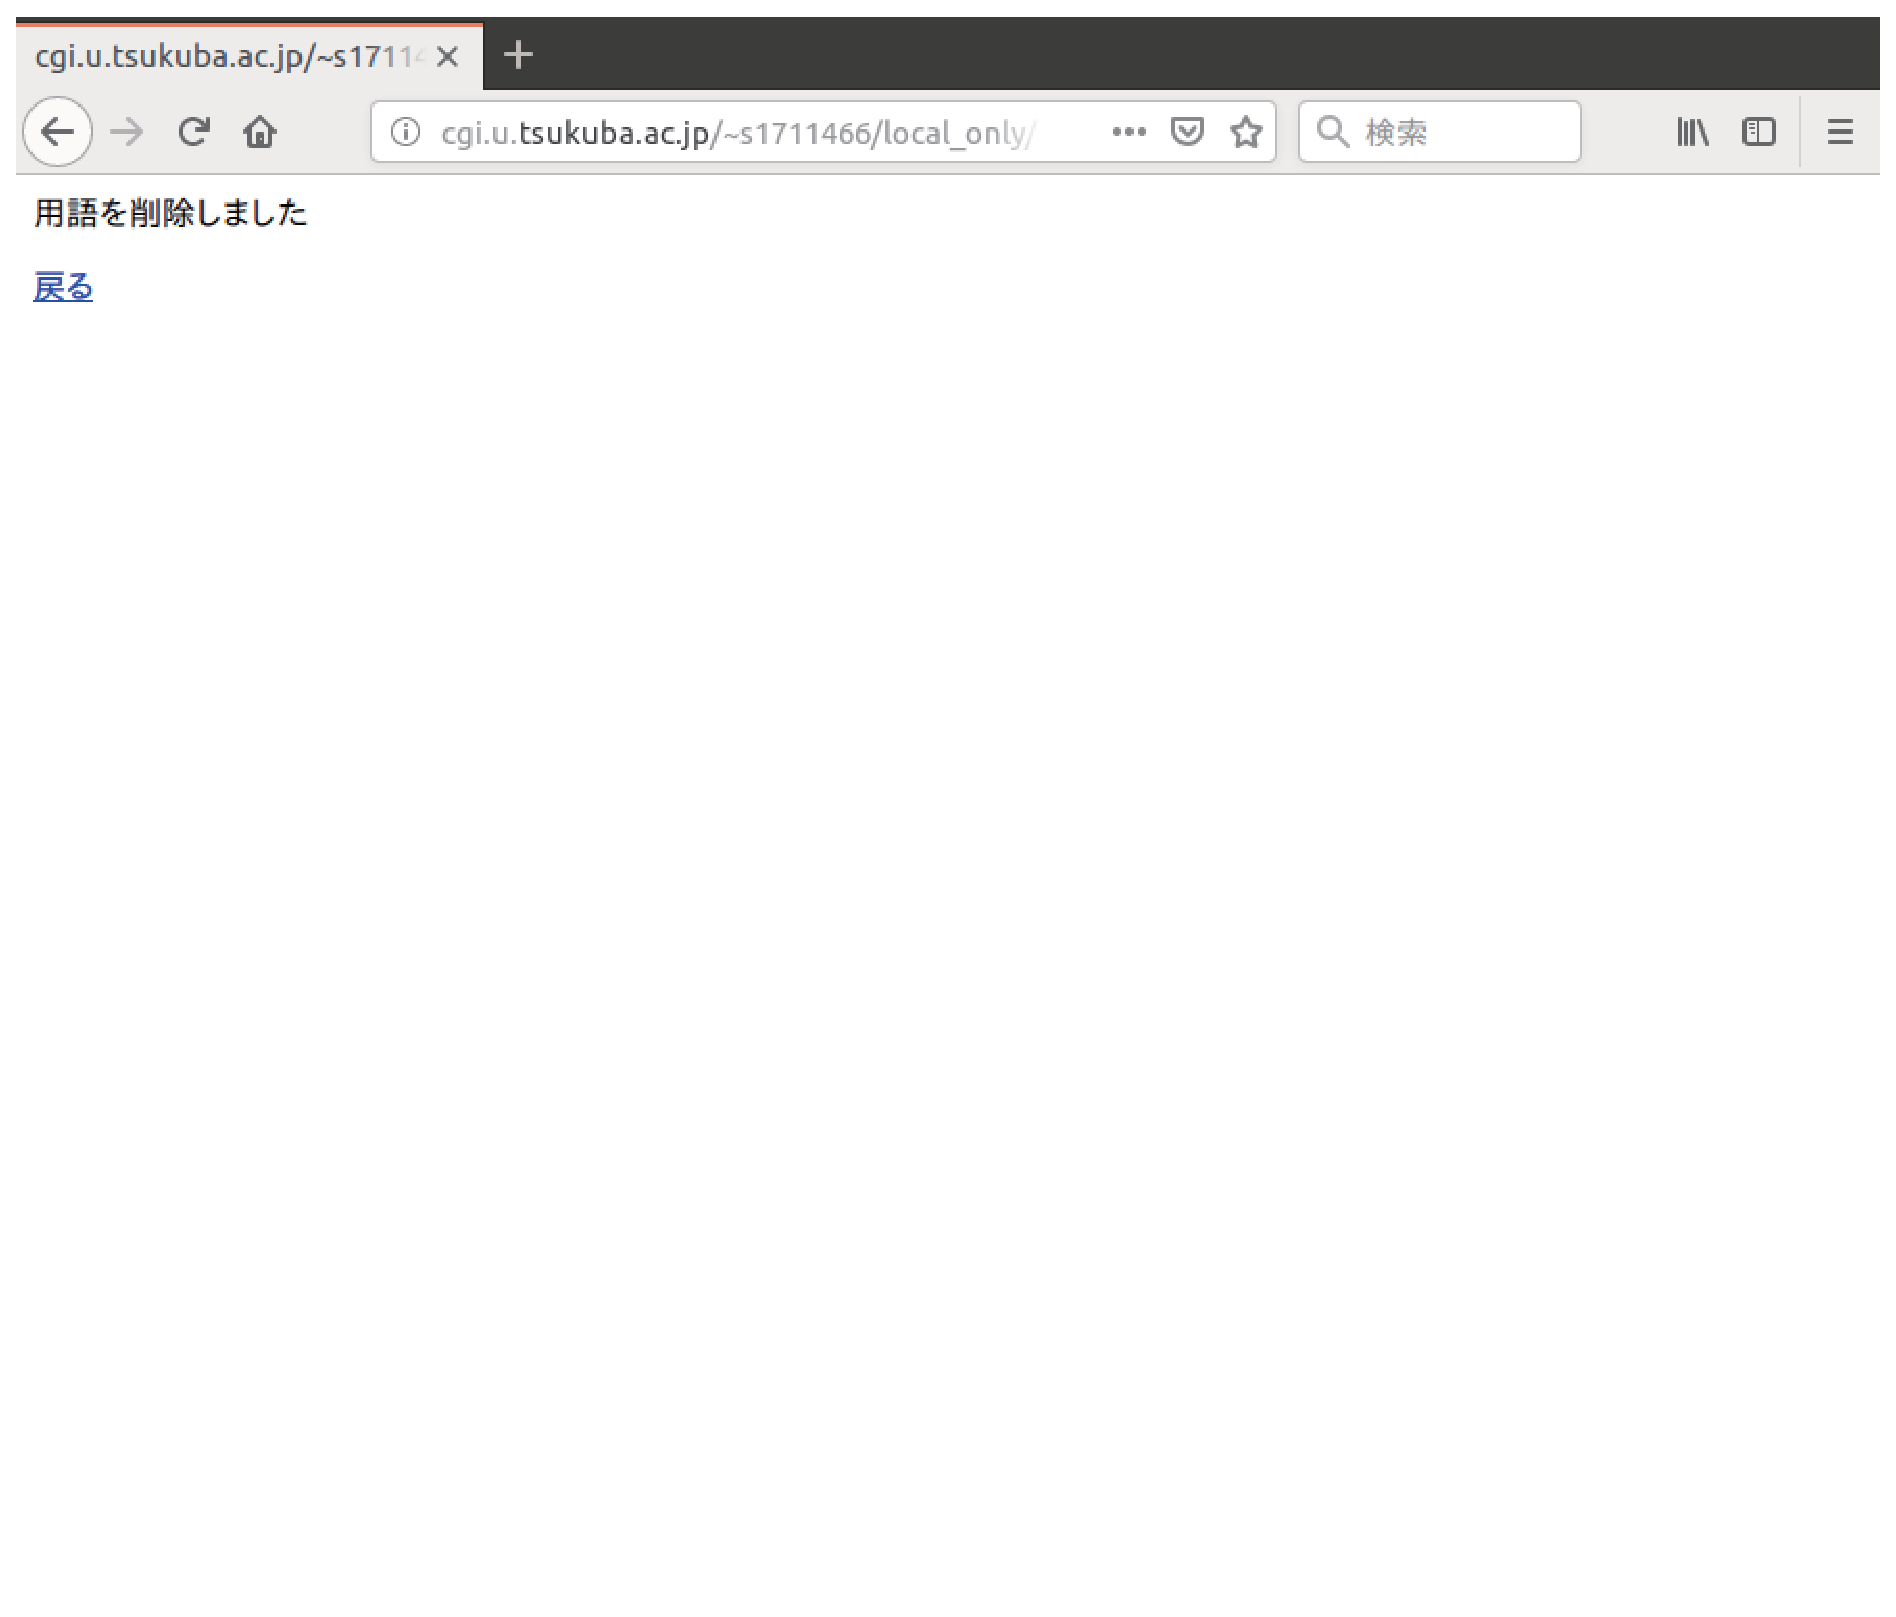
\includegraphics[width=6.7cm]{10-3-19.eps}
          \hspace{1.6cm} [4]削除完了
        \end{center}
      \end{minipage}

      \begin{minipage}{0.55\hsize}
        \vspace{90mm}
      \end{minipage} \\

      % 5
      \begin{minipage}{0.55\hsize}
        \begin{center}
          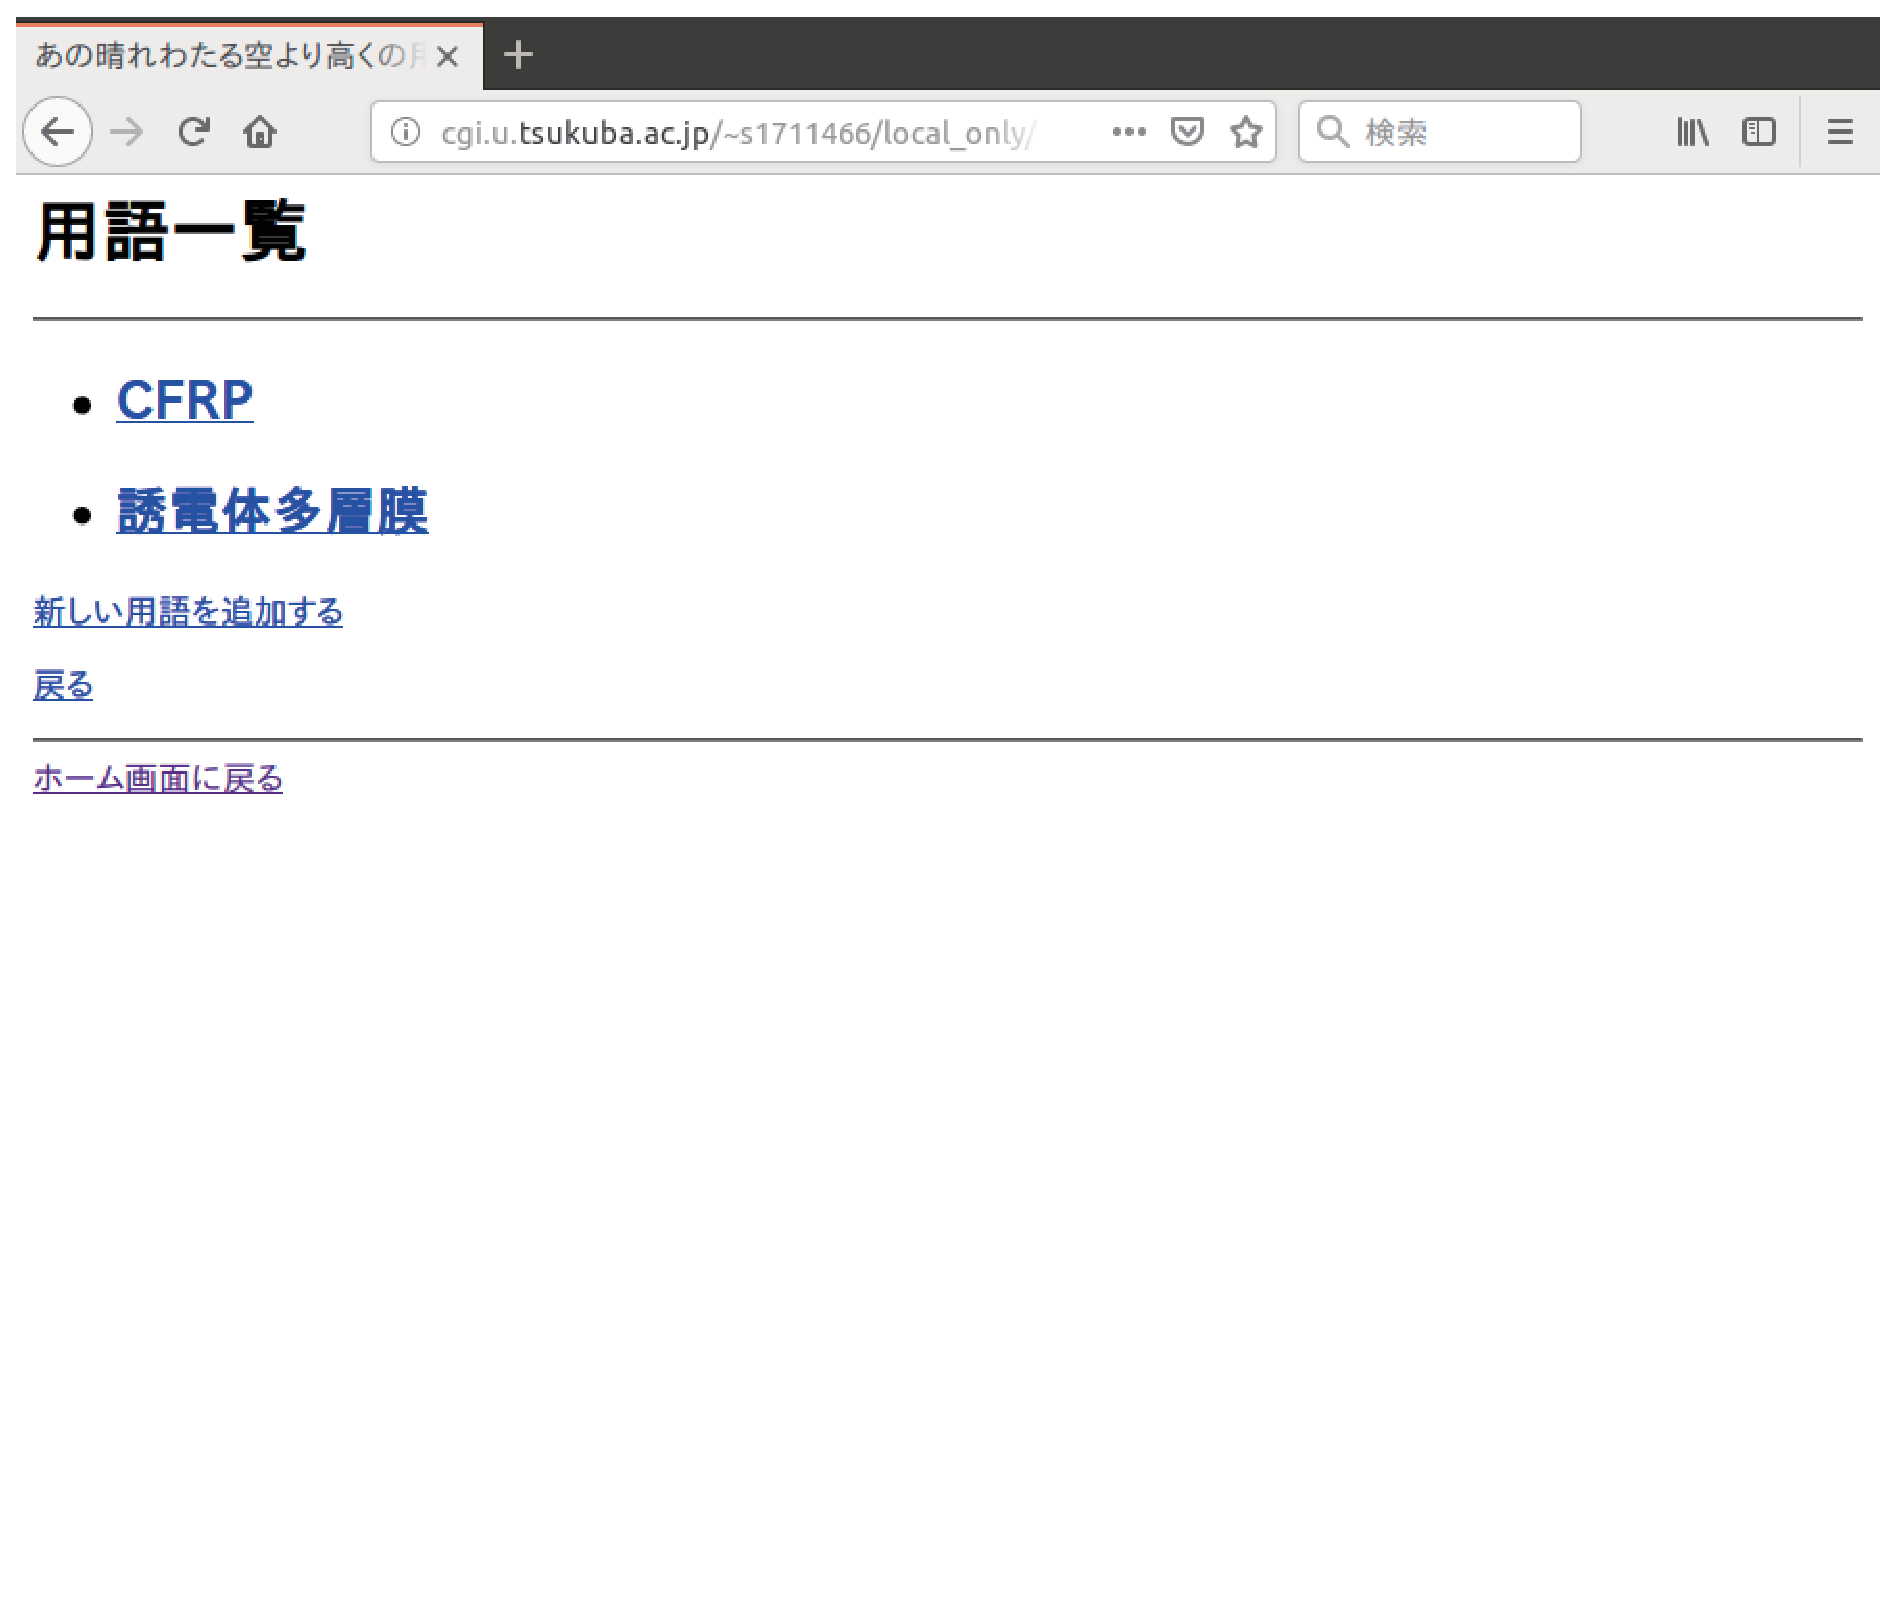
\includegraphics[width=6.7cm]{10-3-20.eps}
          \hspace{1.6cm} [5]内容削除後の用語一覧のページ
        \end{center}
      \end{minipage}

    \end{tabular}
    \caption{用語の削除関係の動作画面}
    \label{fig:b}
  \end{center}
\end{figure}

\begin{figure}[htbp]
  \begin{center}
    \begin{tabular}{c}

      % 1 ホーム画面
      \begin{minipage}{0.55\hsize}
        \begin{center}
          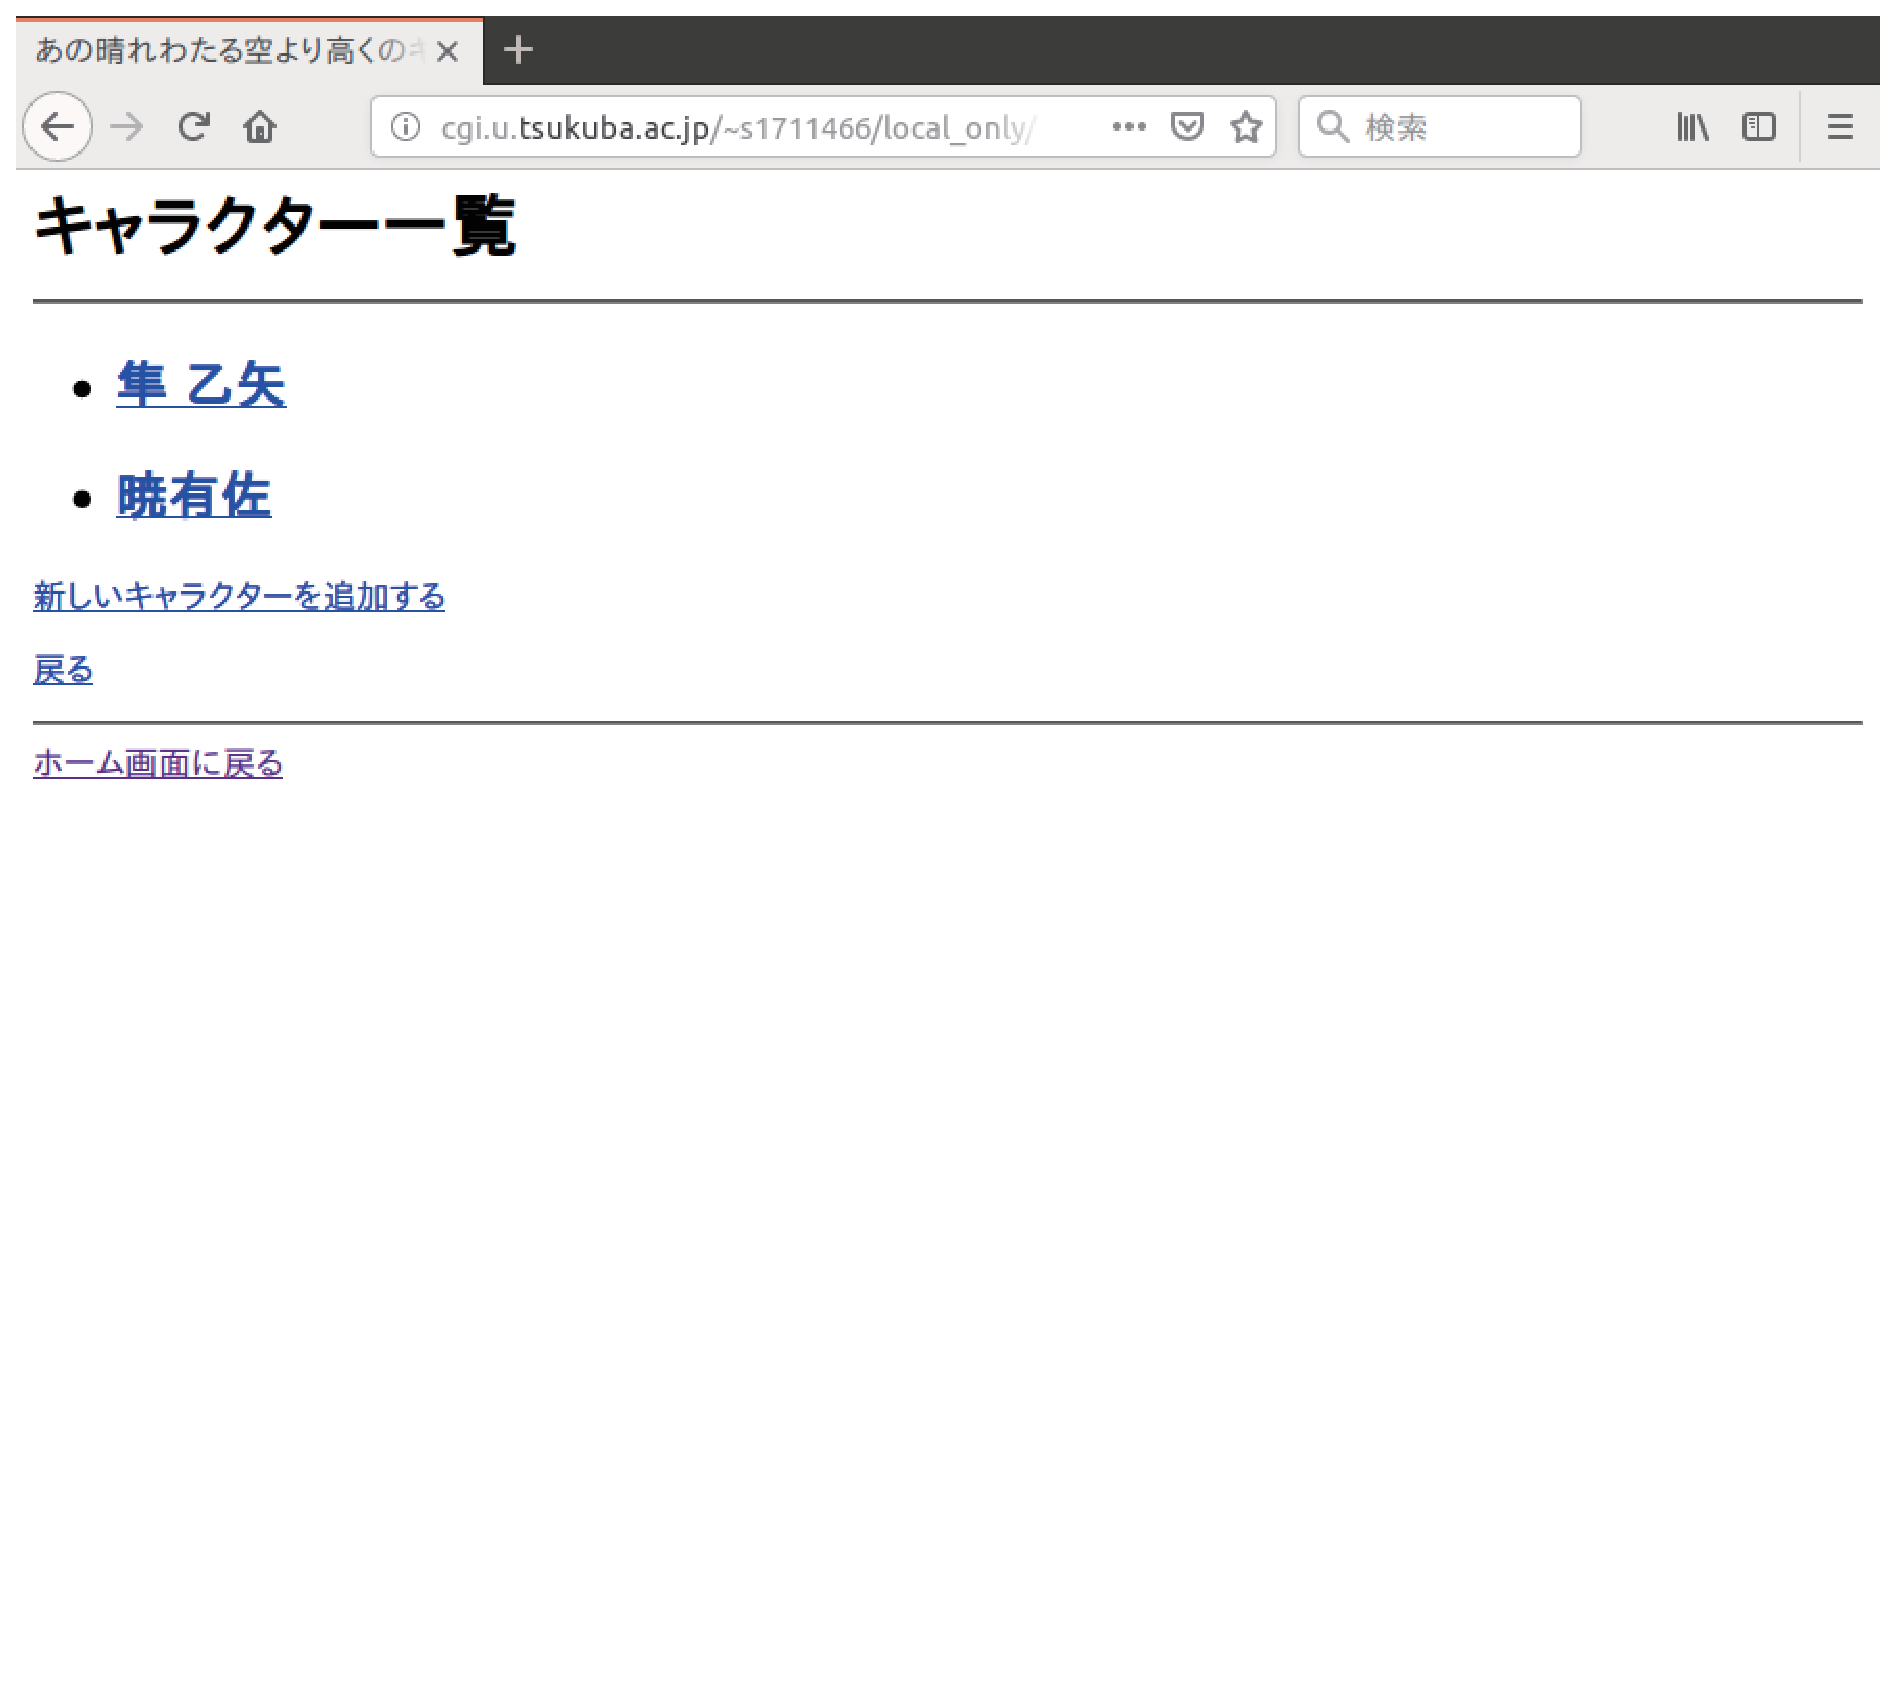
\includegraphics[width=7.0cm]{10-3-21.eps}
          \hspace{1.6cm} [1]キャラクター一覧
        \end{center}
      \end{minipage}

      % 2 
      \begin{minipage}{0.55\hsize}
        \begin{center}
          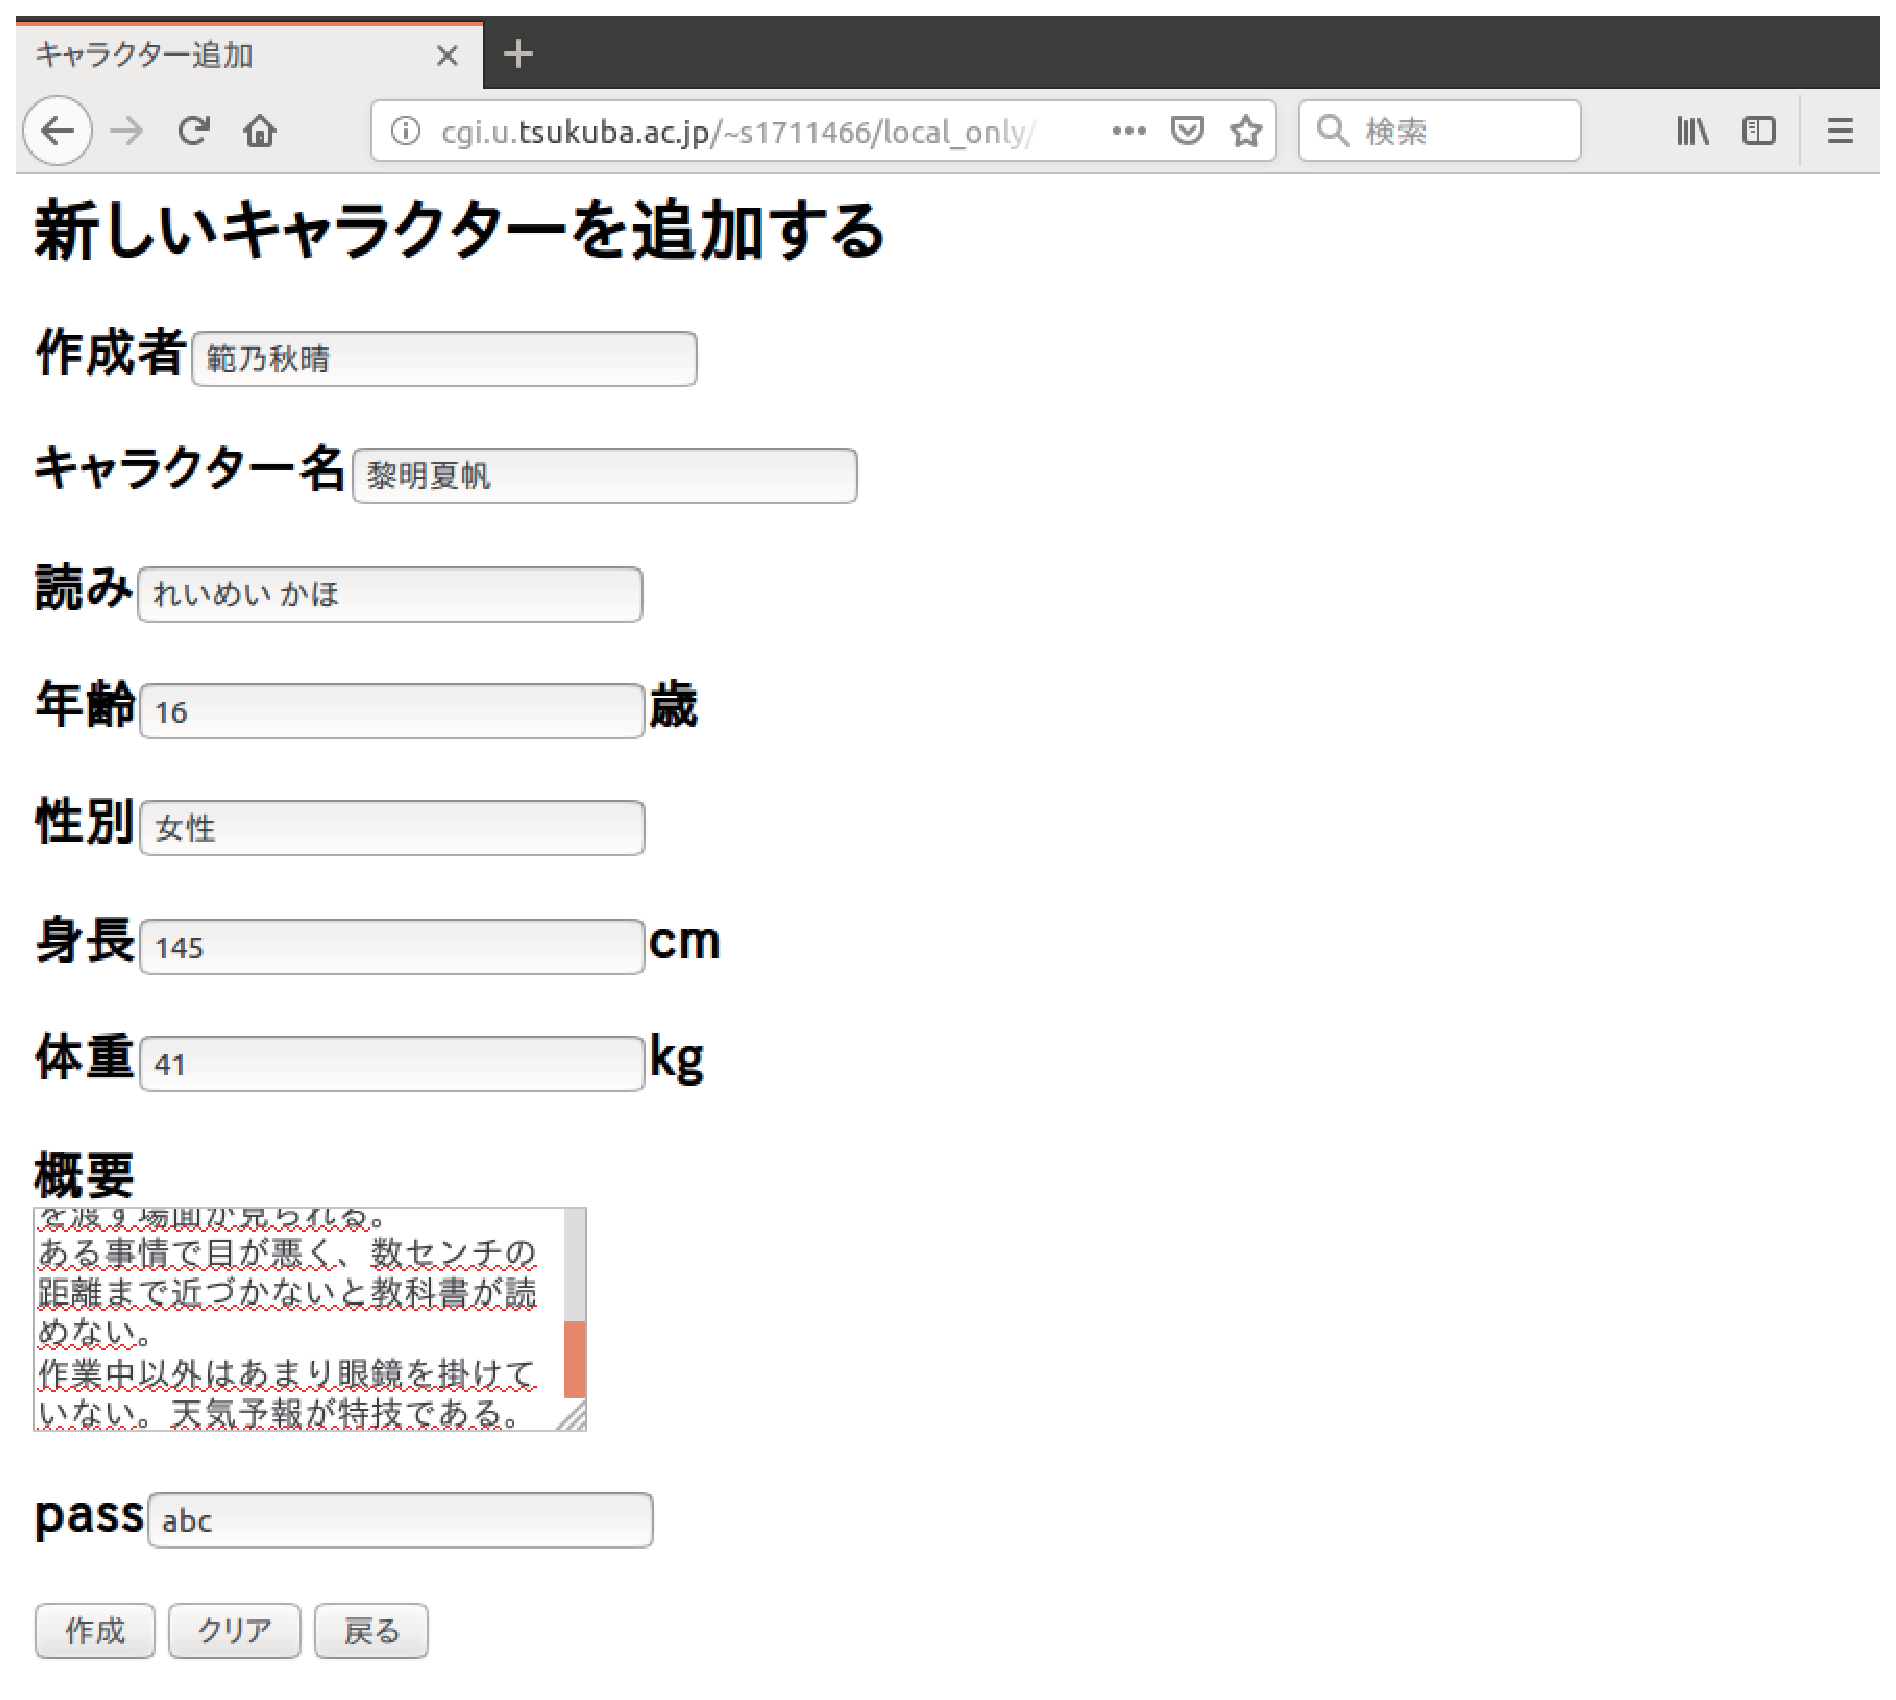
\includegraphics[width=6.7cm]{10-3-22.eps}
          \hspace{1.6cm} [2]新しいキャラクターを追加する
        \end{center}
      \end{minipage}

      \begin{minipage}{0.55\hsize}
        \vspace{30mm}
      \end{minipage} \\
 
      % 3
      \begin{minipage}{0.5\hsize}
        \begin{center}
          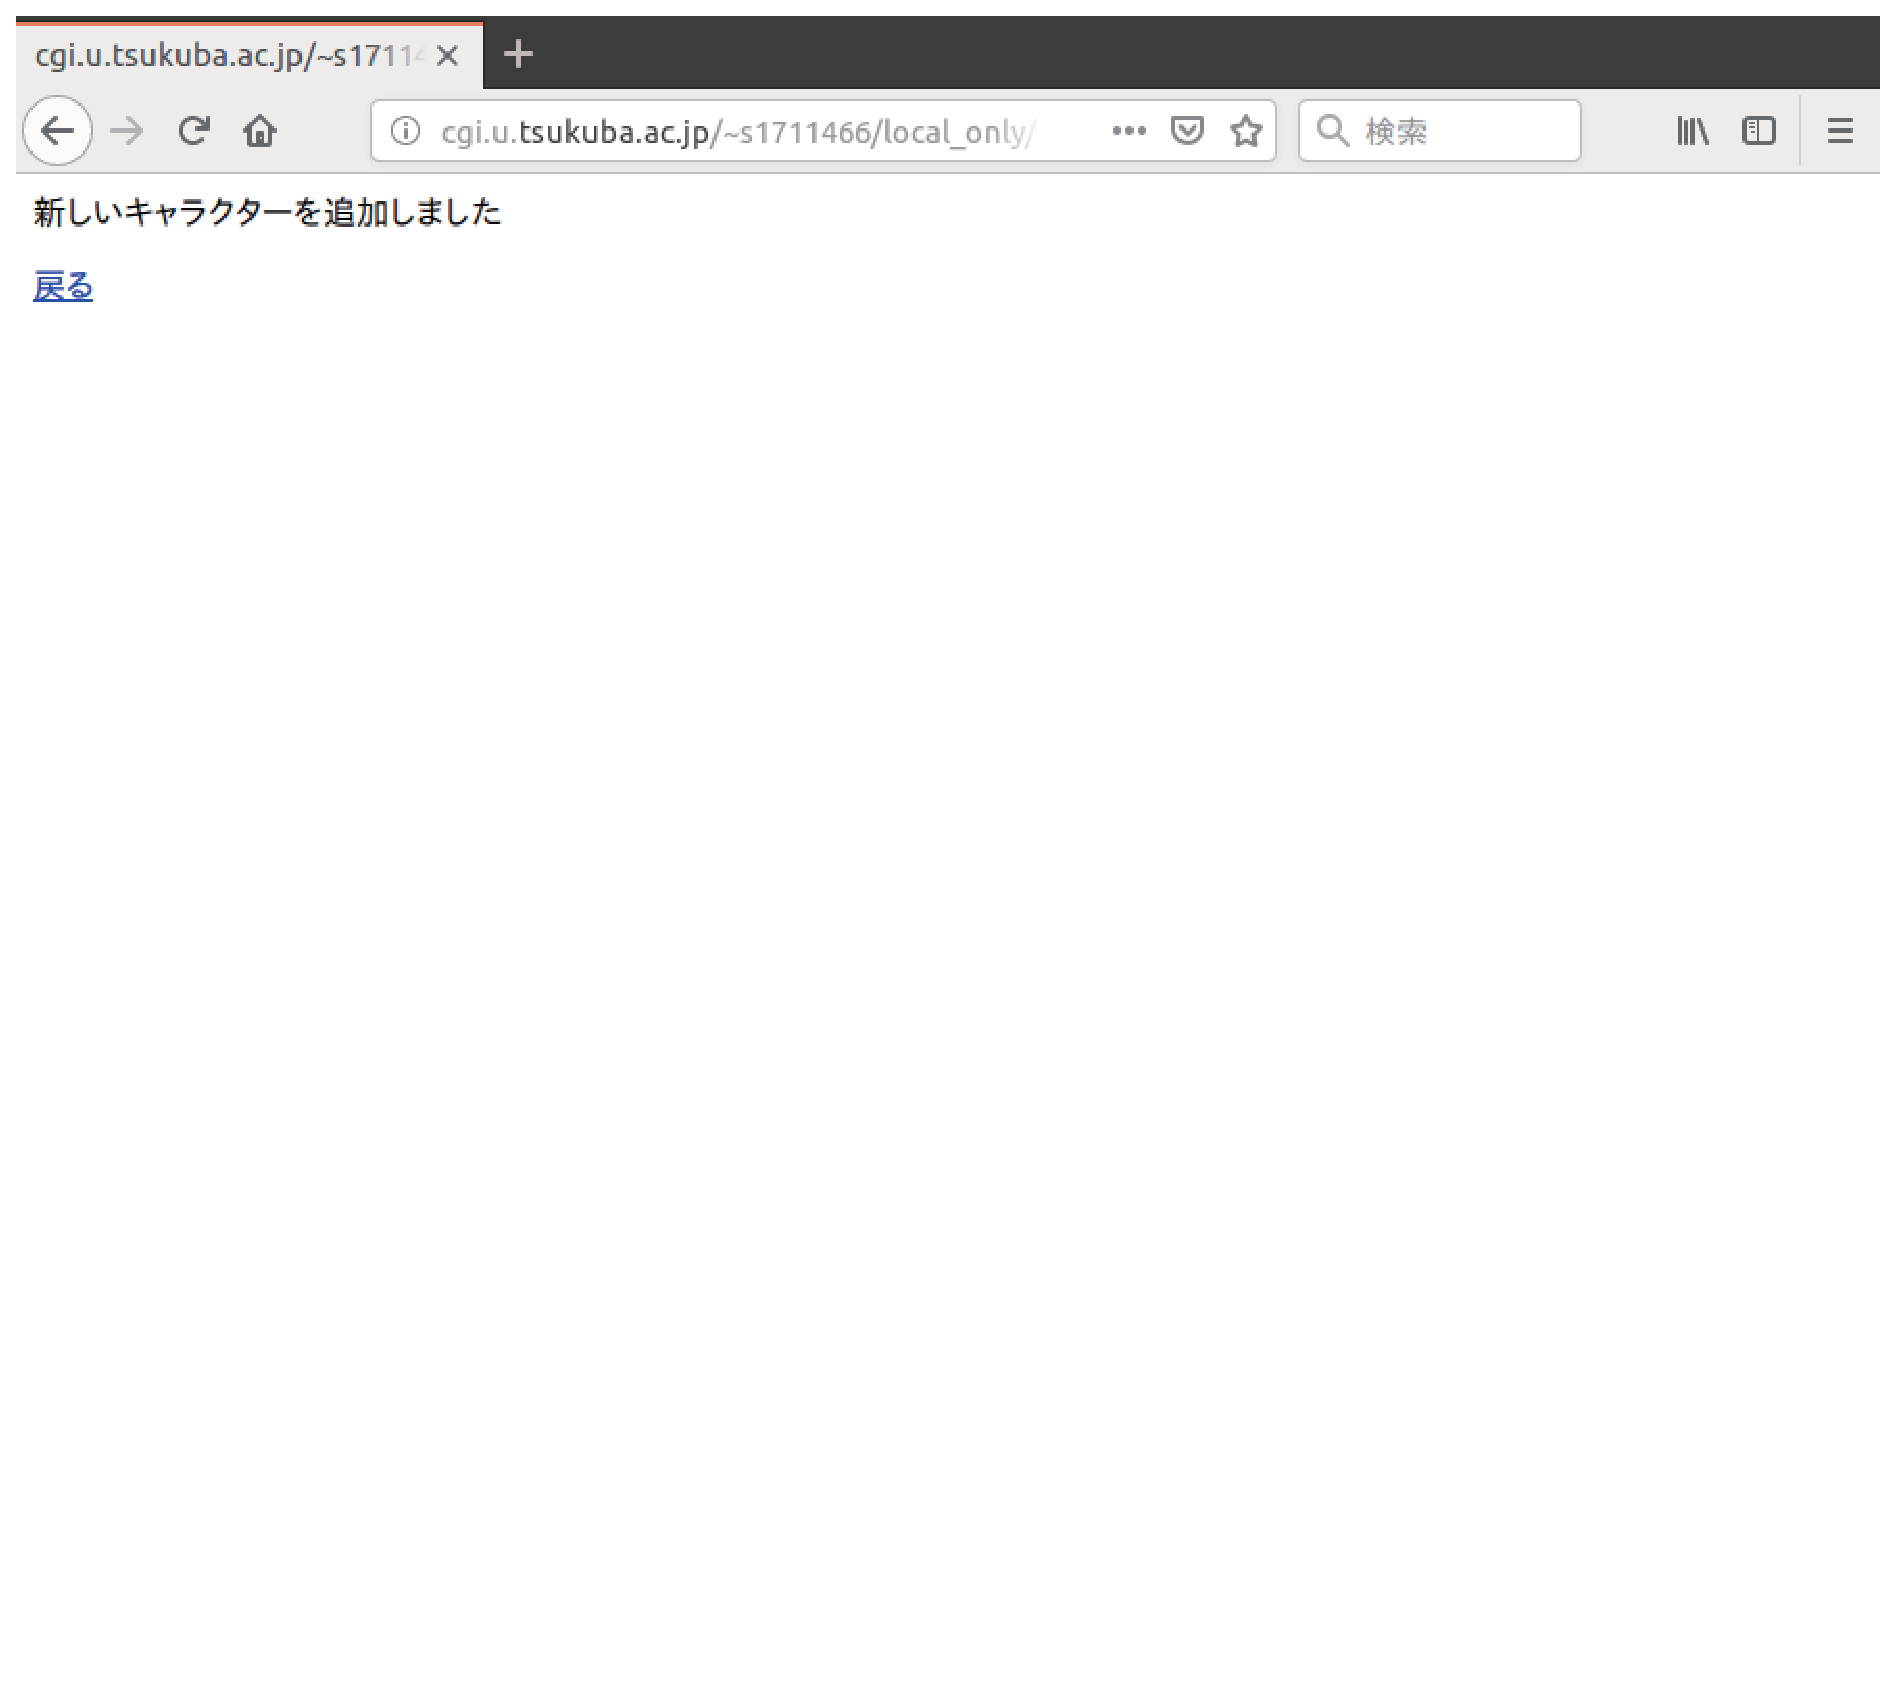
\includegraphics[width=6.7cm]{10-3-23.eps}
          \hspace{1.6cm} [3]追加完了
        \end{center}
      \end{minipage}

      % 4
      \begin{minipage}{0.55\hsize}
        \begin{center}
          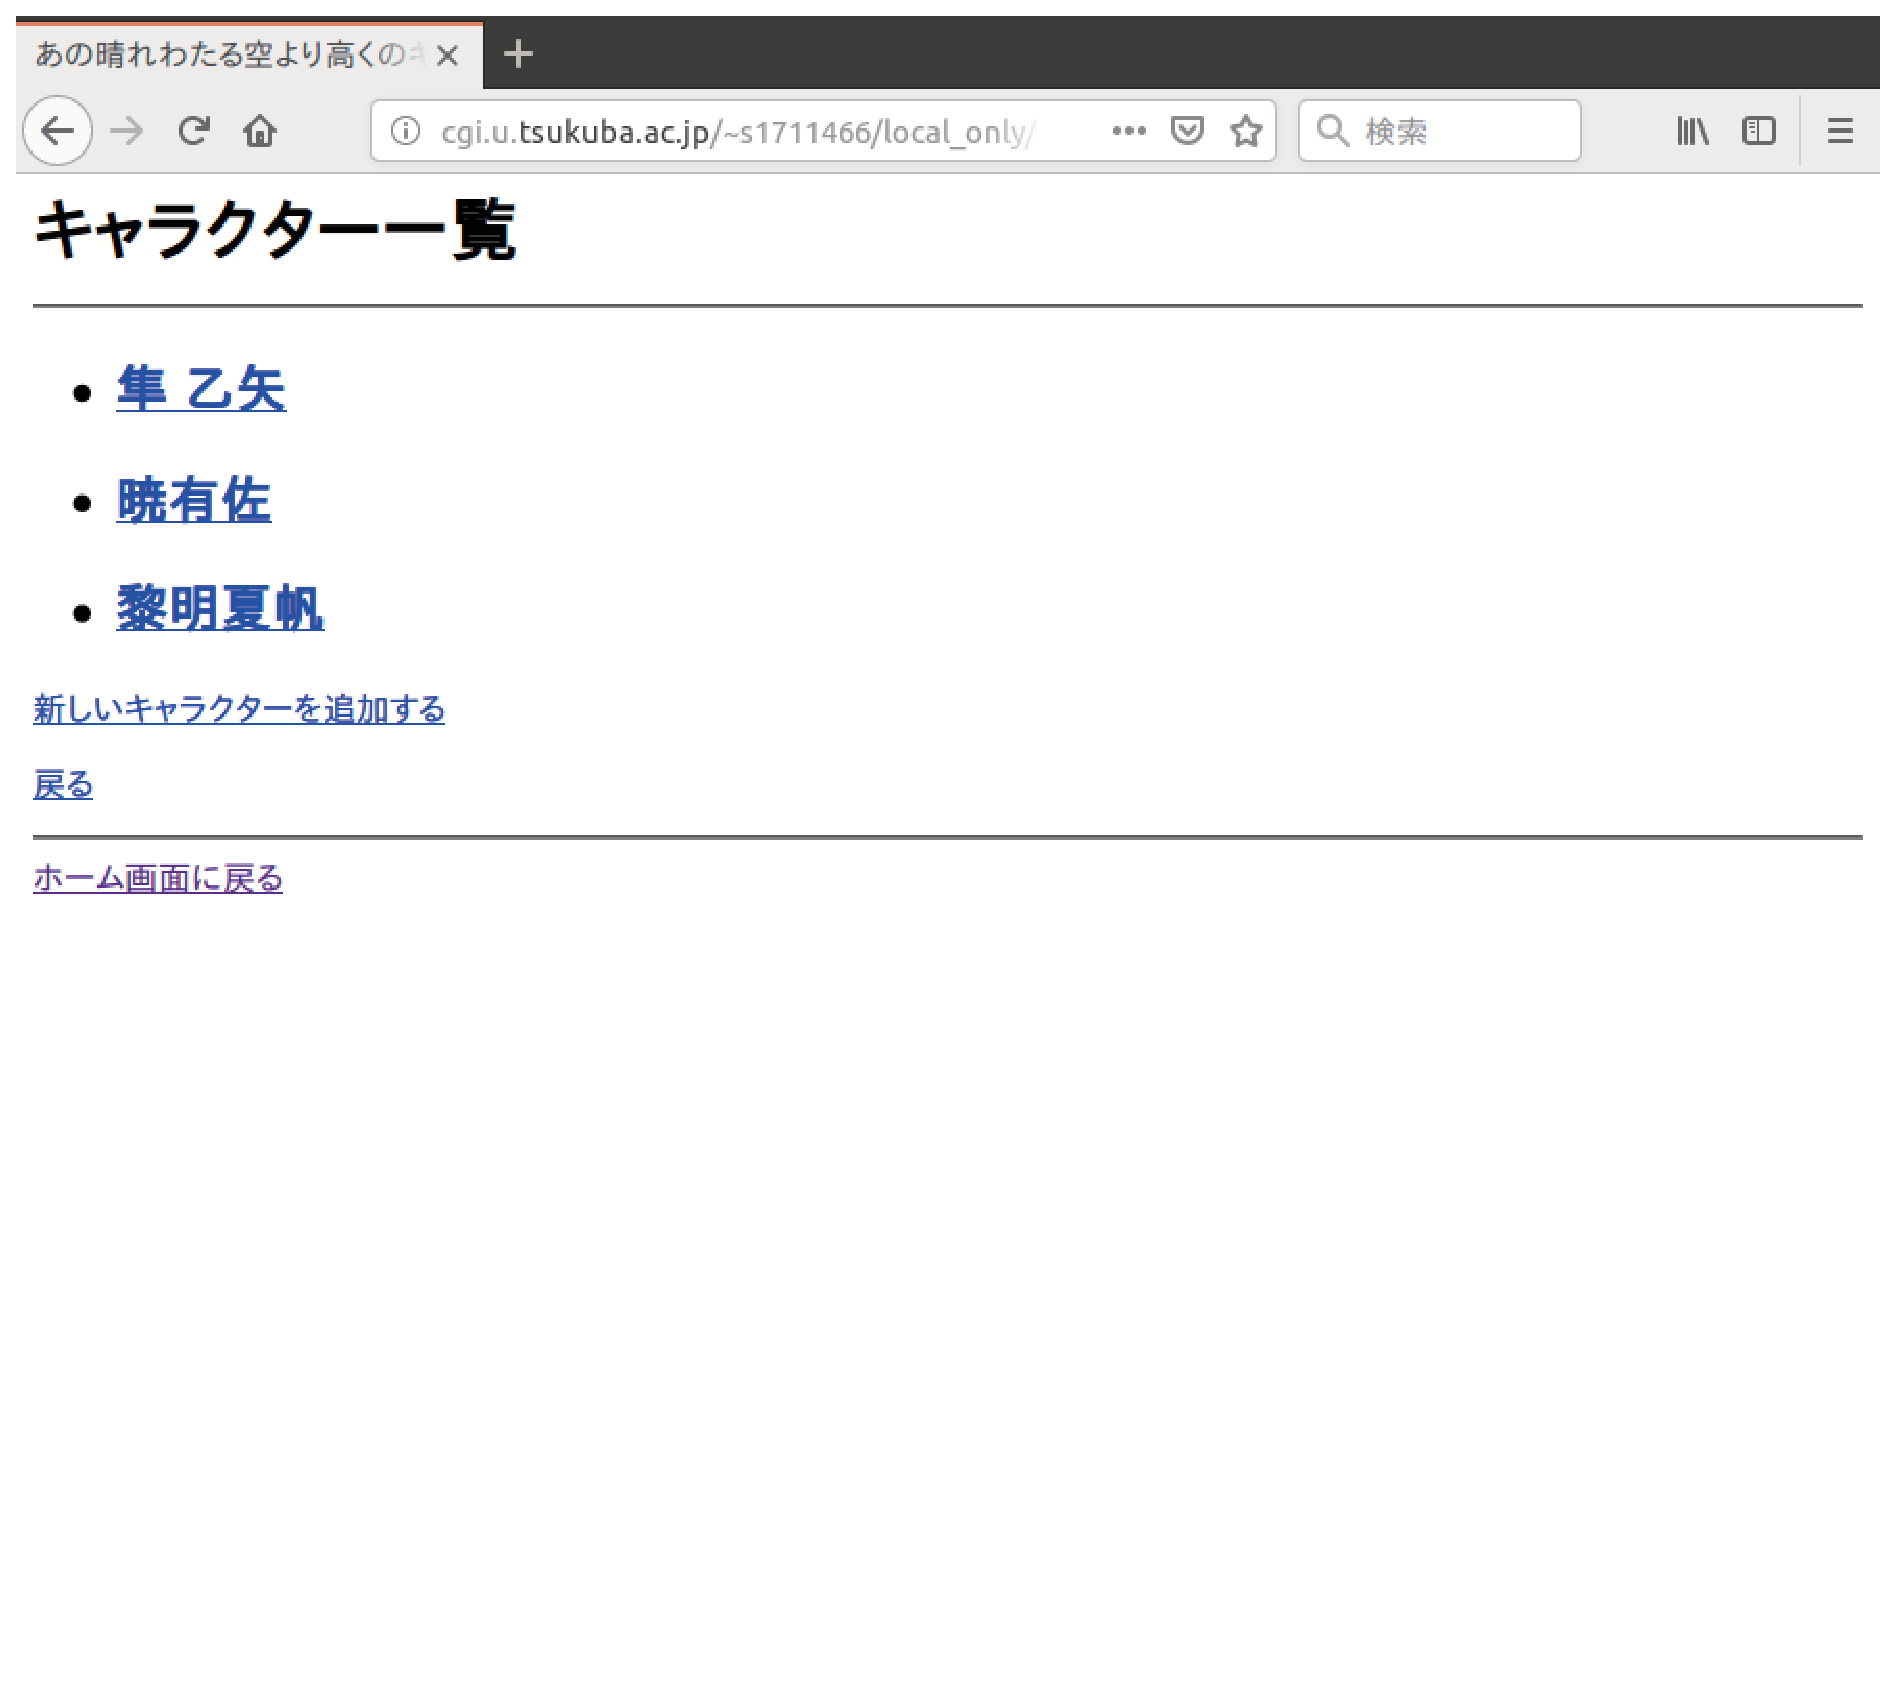
\includegraphics[width=6.7cm]{10-3-24.eps}
          \hspace{1.6cm} [4]新しい用語追加後のキャラクター一覧
        \end{center}
      \end{minipage}

    \end{tabular}
    \caption{キャラクター一覧及び追加関係の動作画面}
    \label{fig:b}
  \end{center}
\end{figure}

\begin{figure}[htbp]
  \begin{center}
    \begin{tabular}{c}

      % 1 ホーム画面
      \begin{minipage}{0.55\hsize}
        \begin{center}
          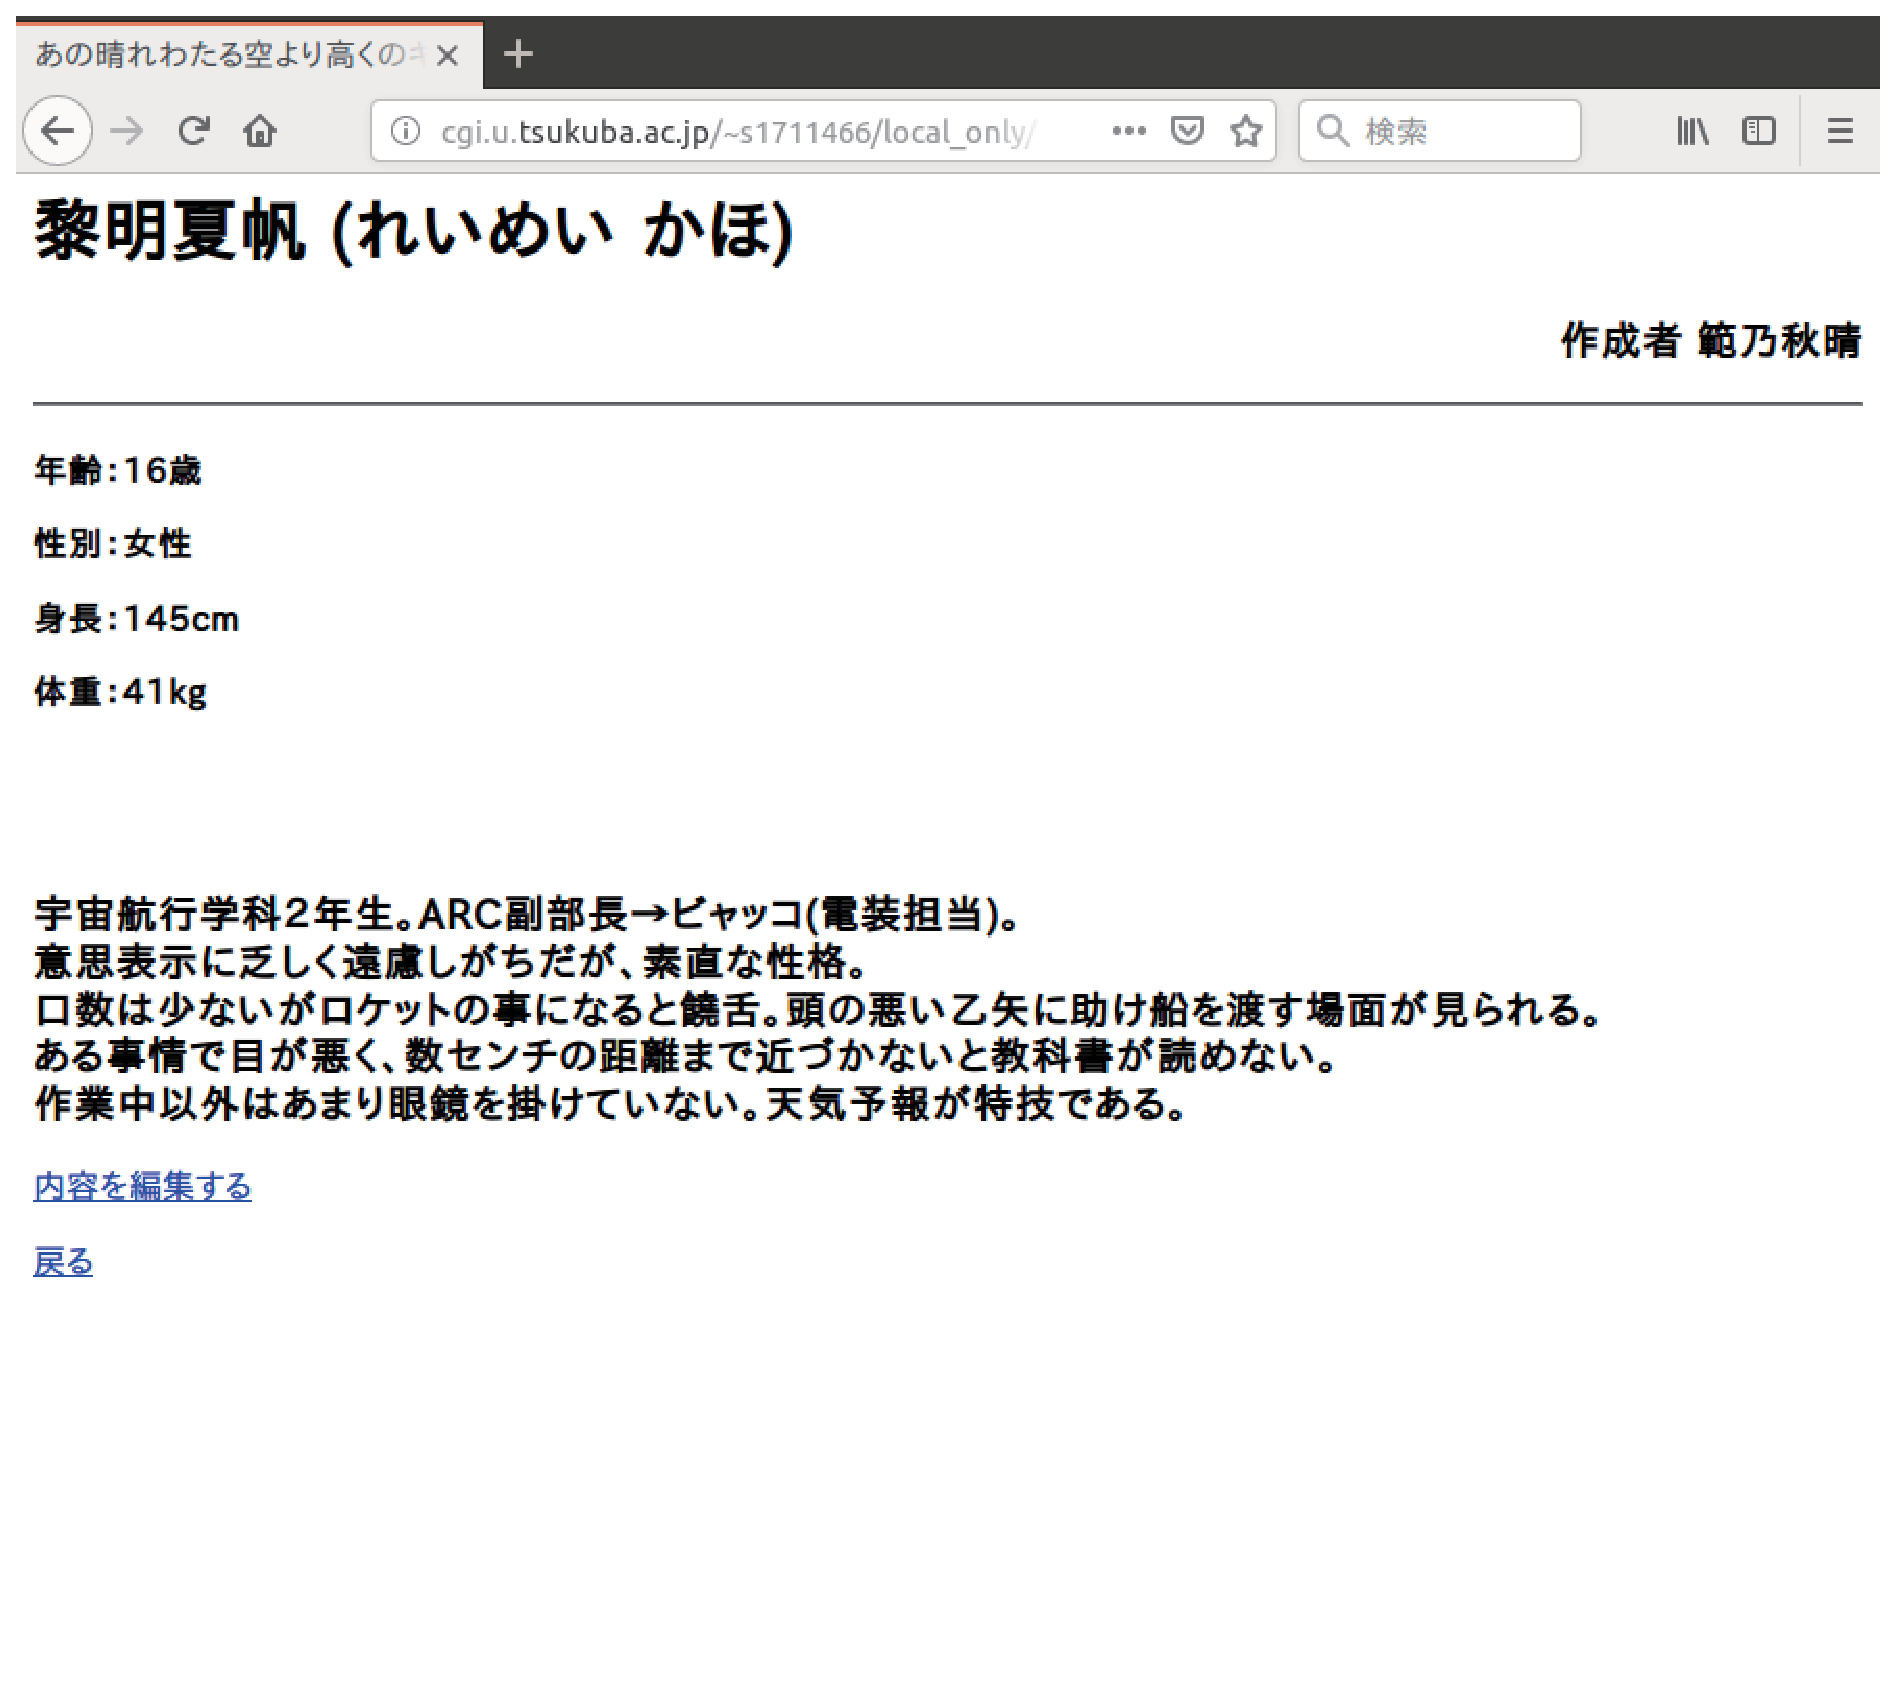
\includegraphics[width=7.0cm]{10-3-25.eps}
          \hspace{1.6cm} [1]キャラクターの個別ページ
        \end{center}
      \end{minipage}

      % 2 
      \begin{minipage}{0.55\hsize}
        \begin{center}
          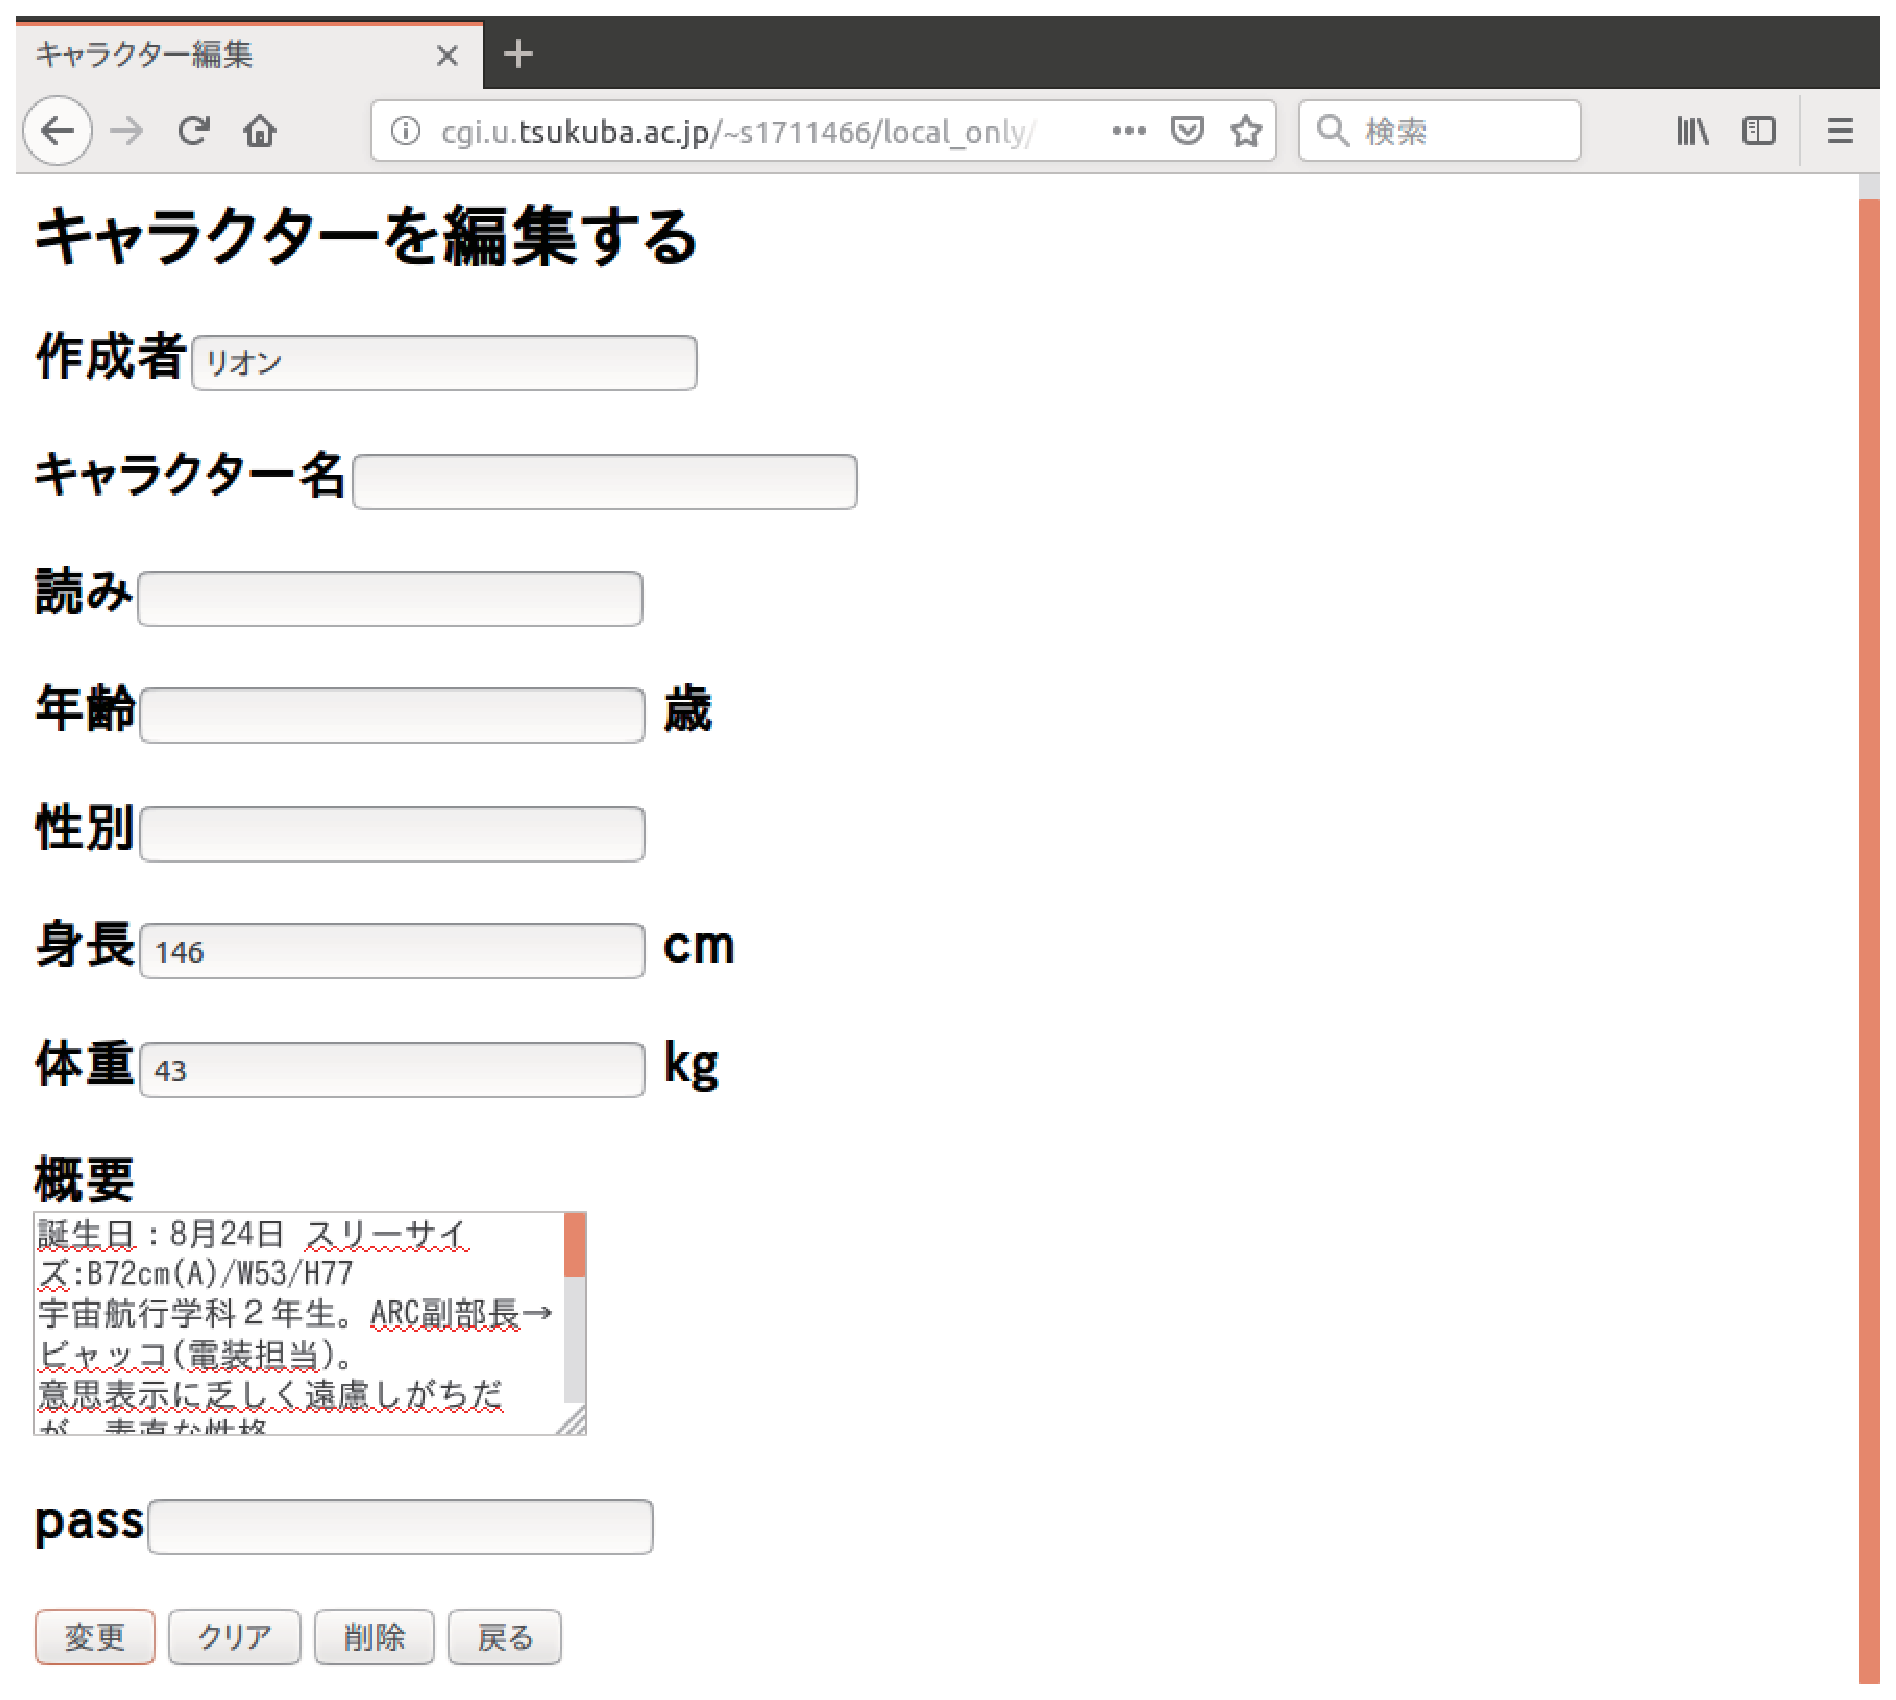
\includegraphics[width=6.7cm]{10-3-26.eps}
          \hspace{1.6cm} [2]キャラクターの内容を編集する
        \end{center}
      \end{minipage}

      \begin{minipage}{0.55\hsize}
        \vspace{30mm}
      \end{minipage} \\
 
      % 3
      \begin{minipage}{0.5\hsize}
        \begin{center}
          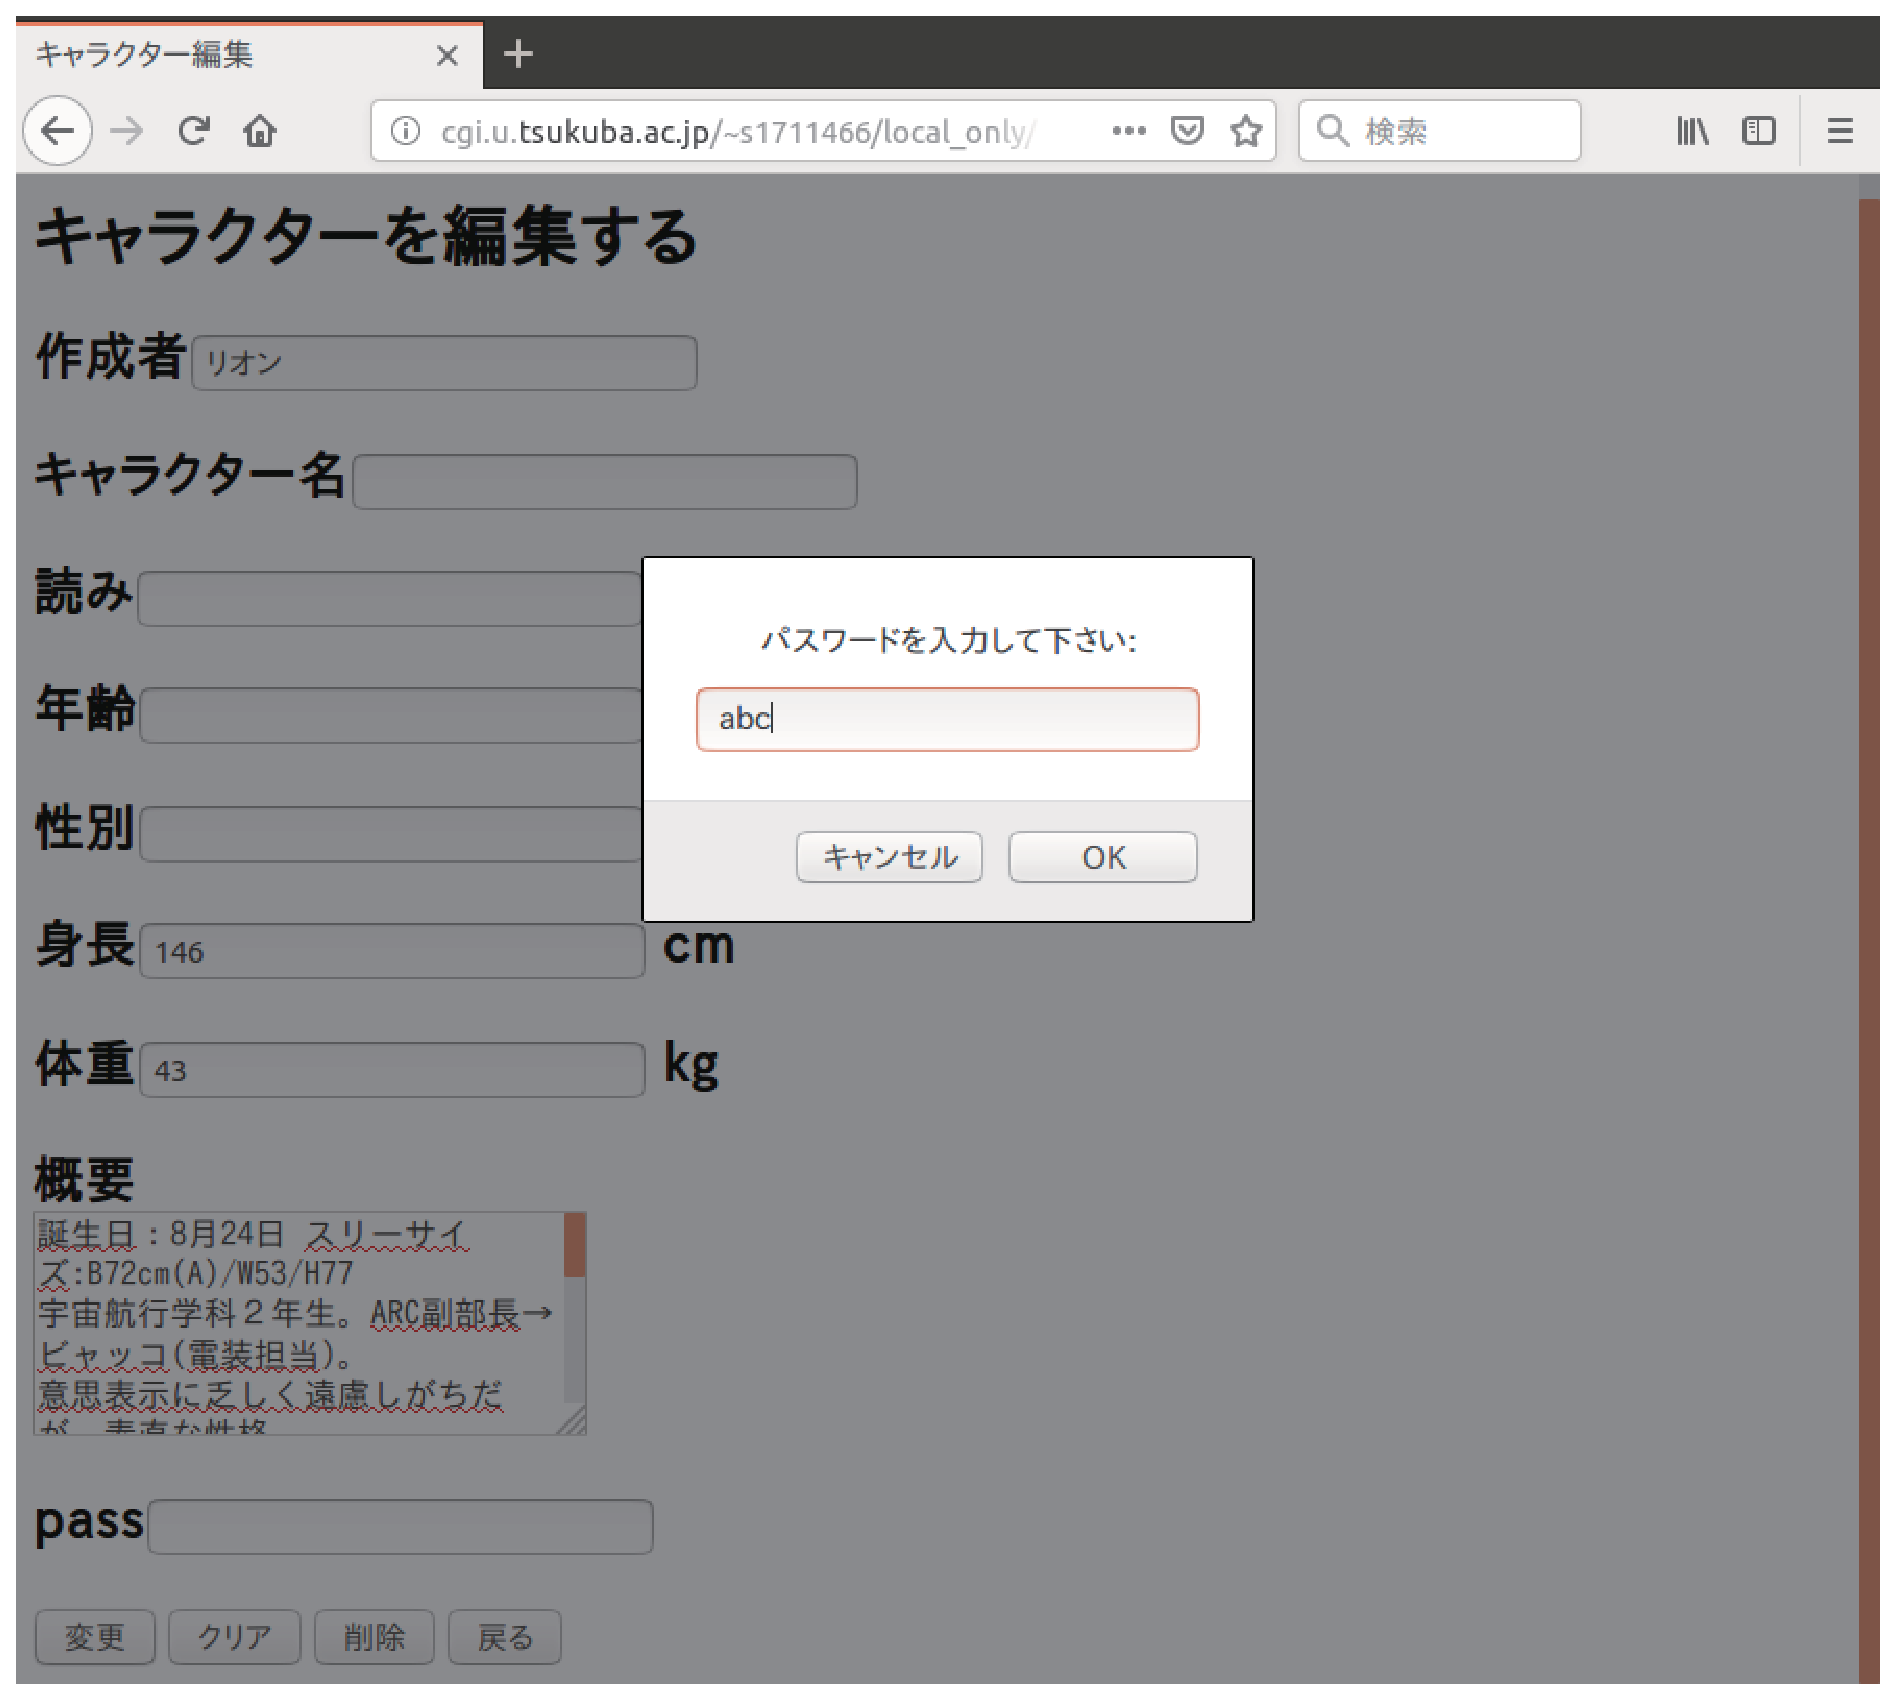
\includegraphics[width=6.7cm]{10-3-27.eps}
          \hspace{1.6cm} [3]パスワード要求
        \end{center}
      \end{minipage}

      % 4
      \begin{minipage}{0.55\hsize}
        \begin{center}
          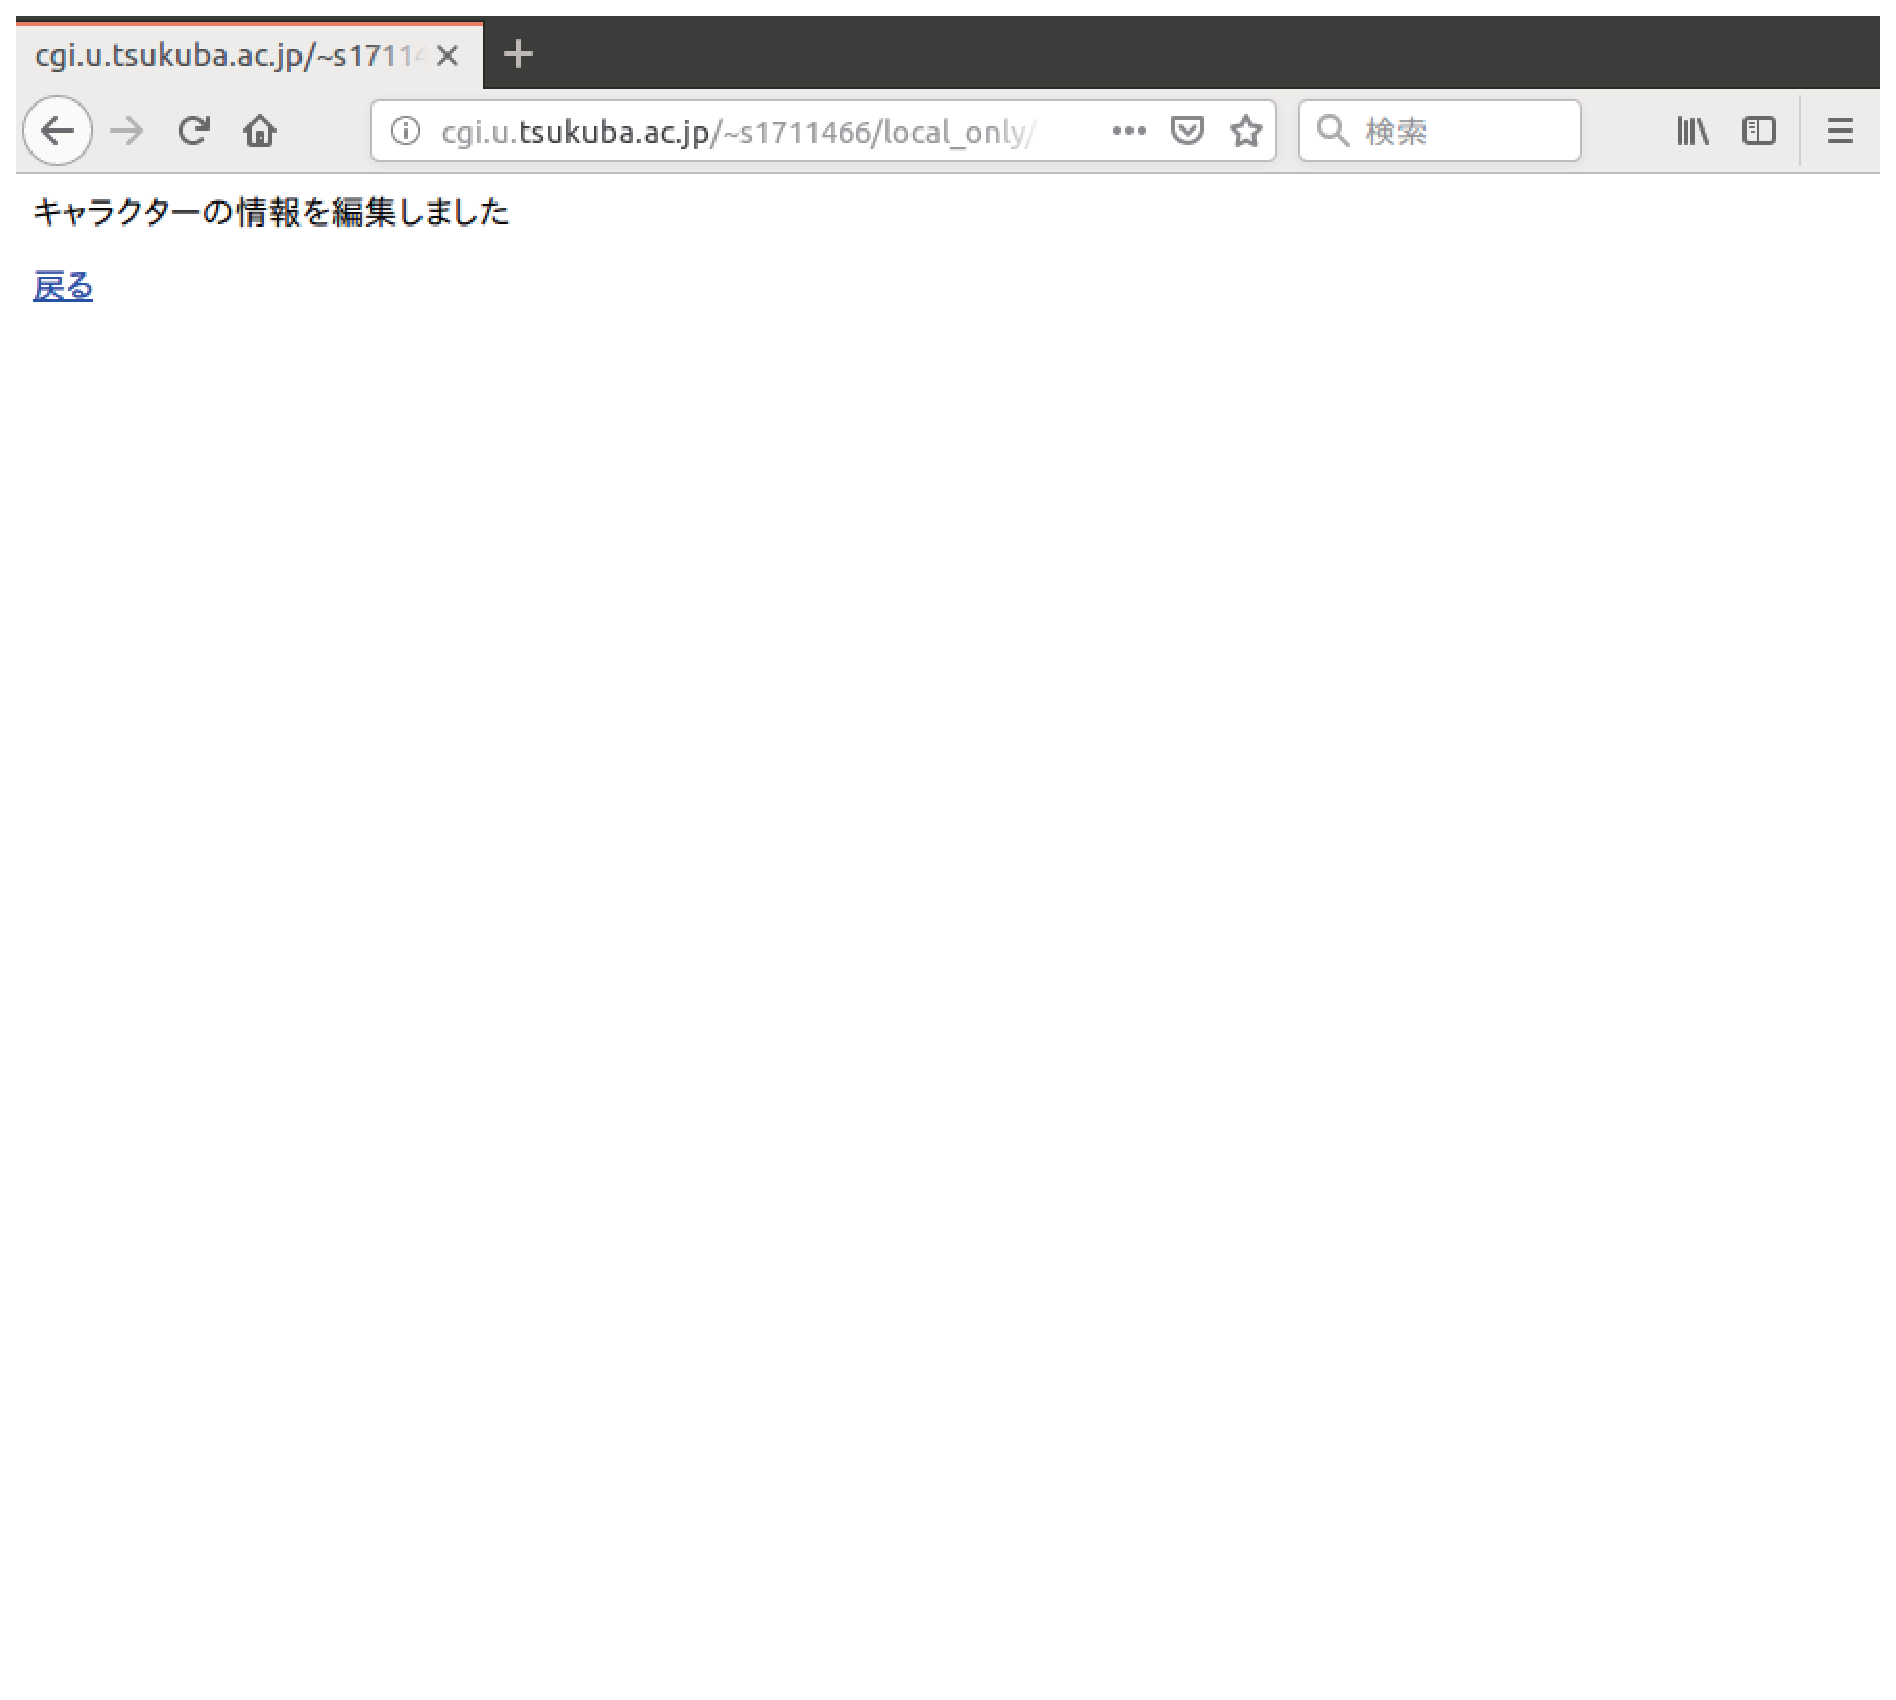
\includegraphics[width=6.7cm]{10-3-28.eps}
          \hspace{1.6cm} [4]編集完了
        \end{center}
      \end{minipage}

      \begin{minipage}{0.55\hsize}
        \vspace{90mm}
      \end{minipage} \\

      % 5
      \begin{minipage}{0.55\hsize}
        \begin{center}
          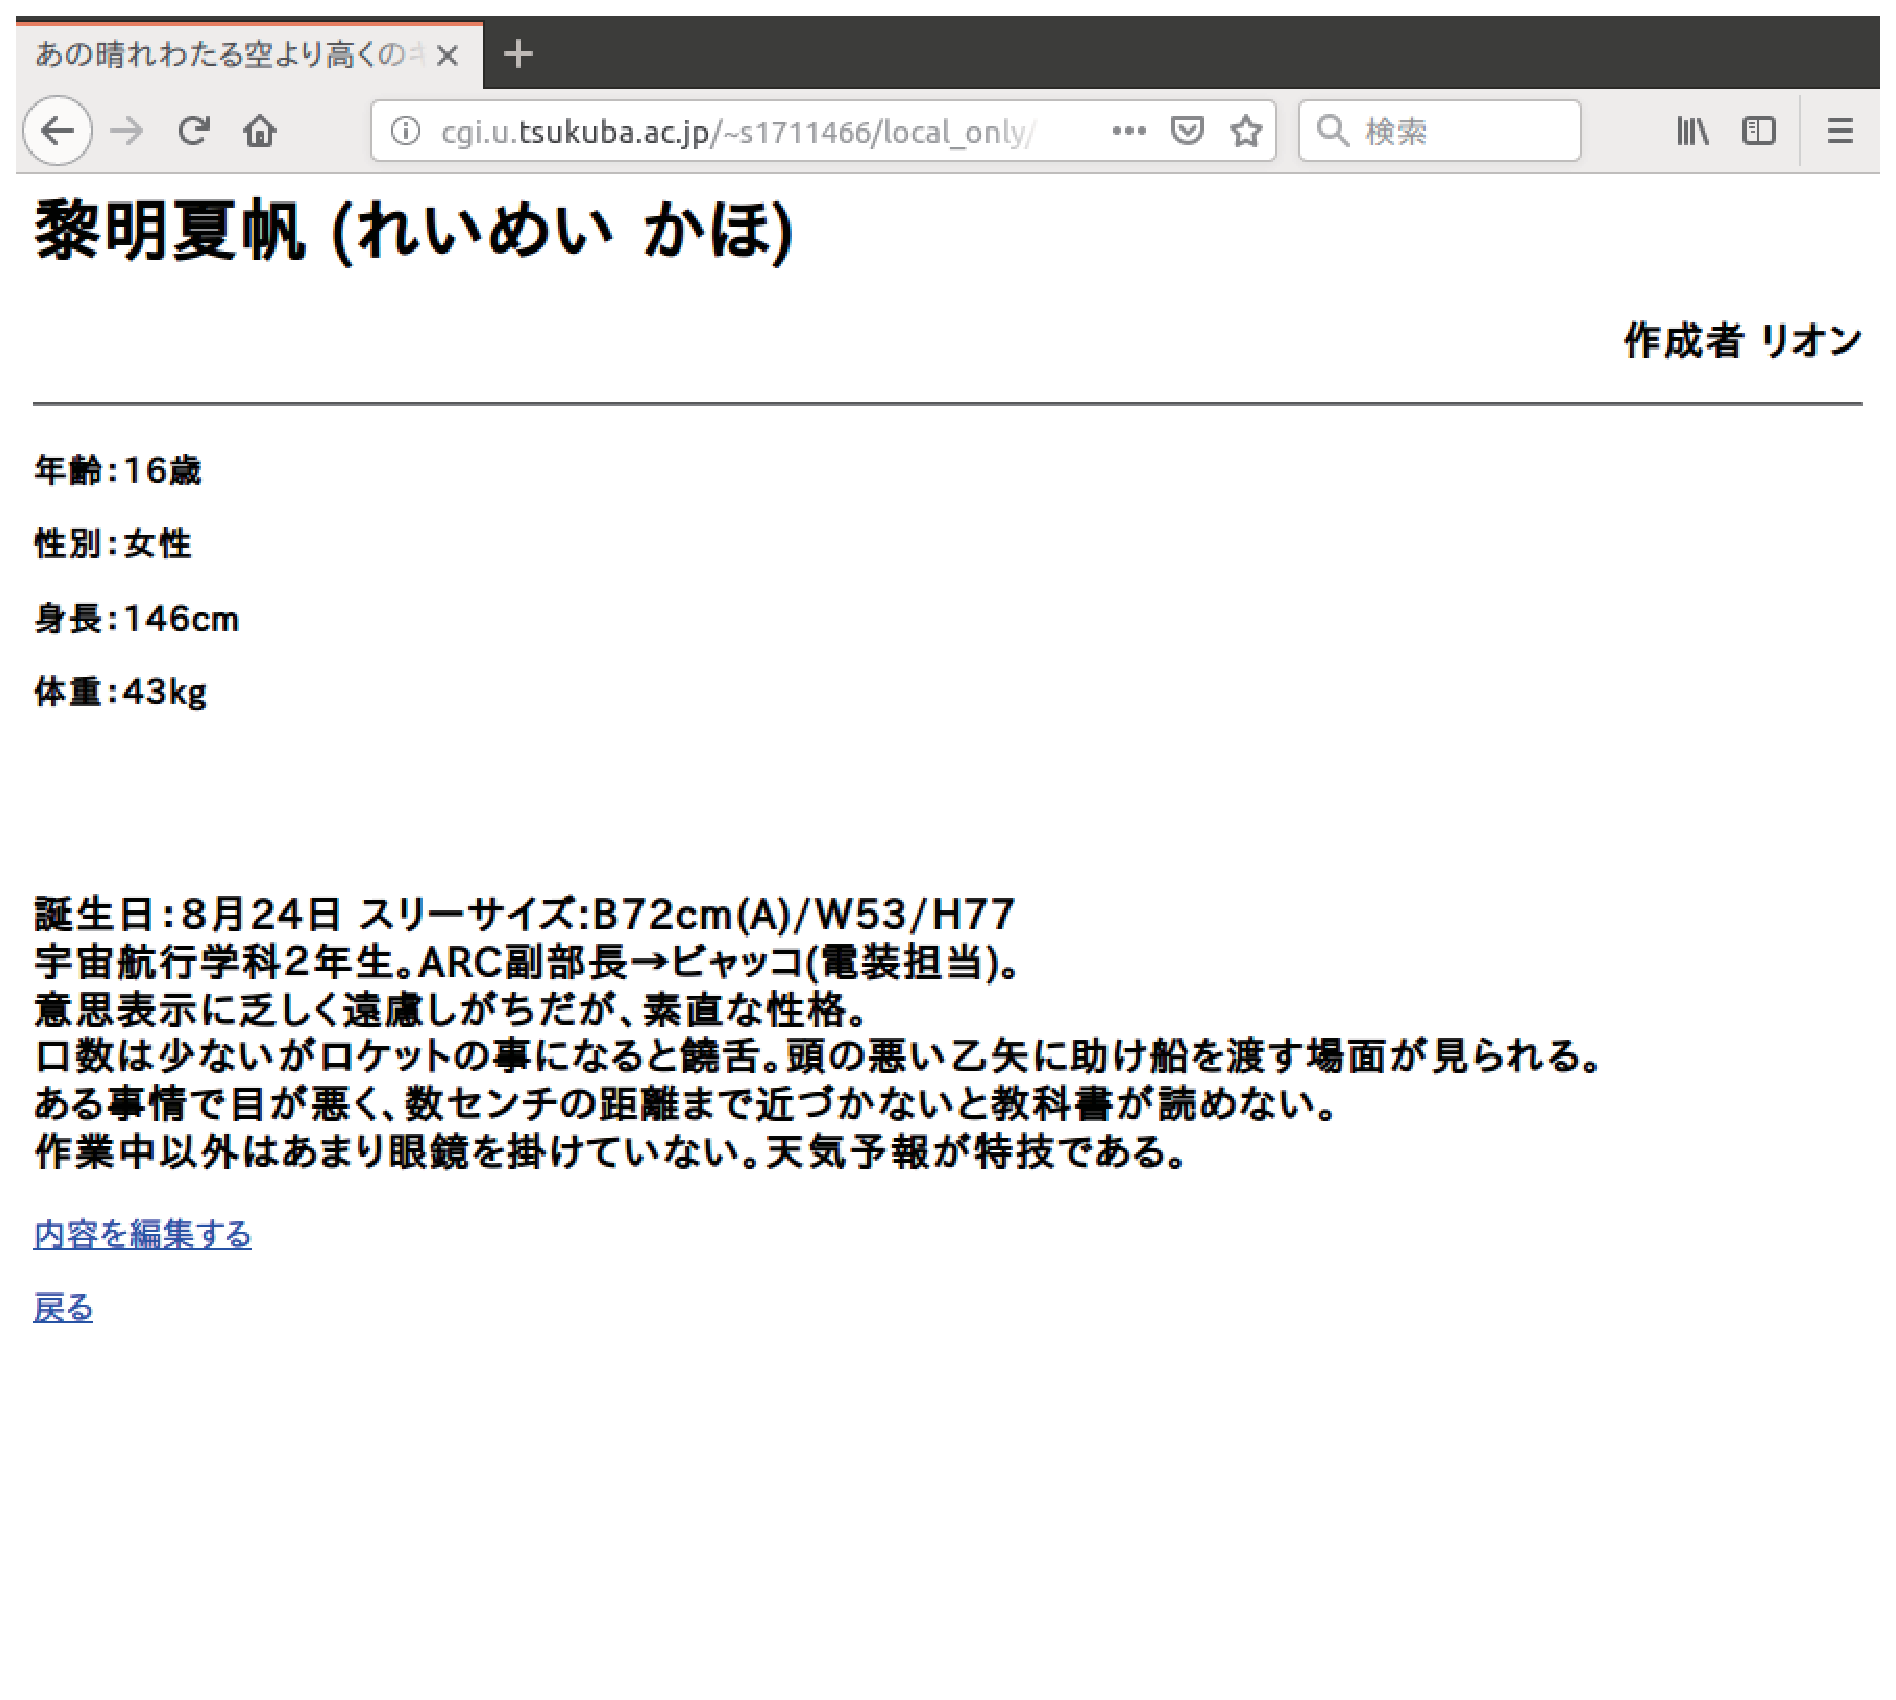
\includegraphics[width=6.7cm]{10-3-29.eps}
          \hspace{1.6cm} [5]内容編集後のキャラクターの個別ページ
        \end{center}
      \end{minipage}

    \end{tabular}
    \caption{キャラクターの編集関係の動作画面}
    \label{fig:b}
  \end{center}
\end{figure}

\begin{figure}[htbp]
  \begin{center}
    \begin{tabular}{c}

      % 1 ホーム画面
      \begin{minipage}{0.55\hsize}
        \begin{center}
          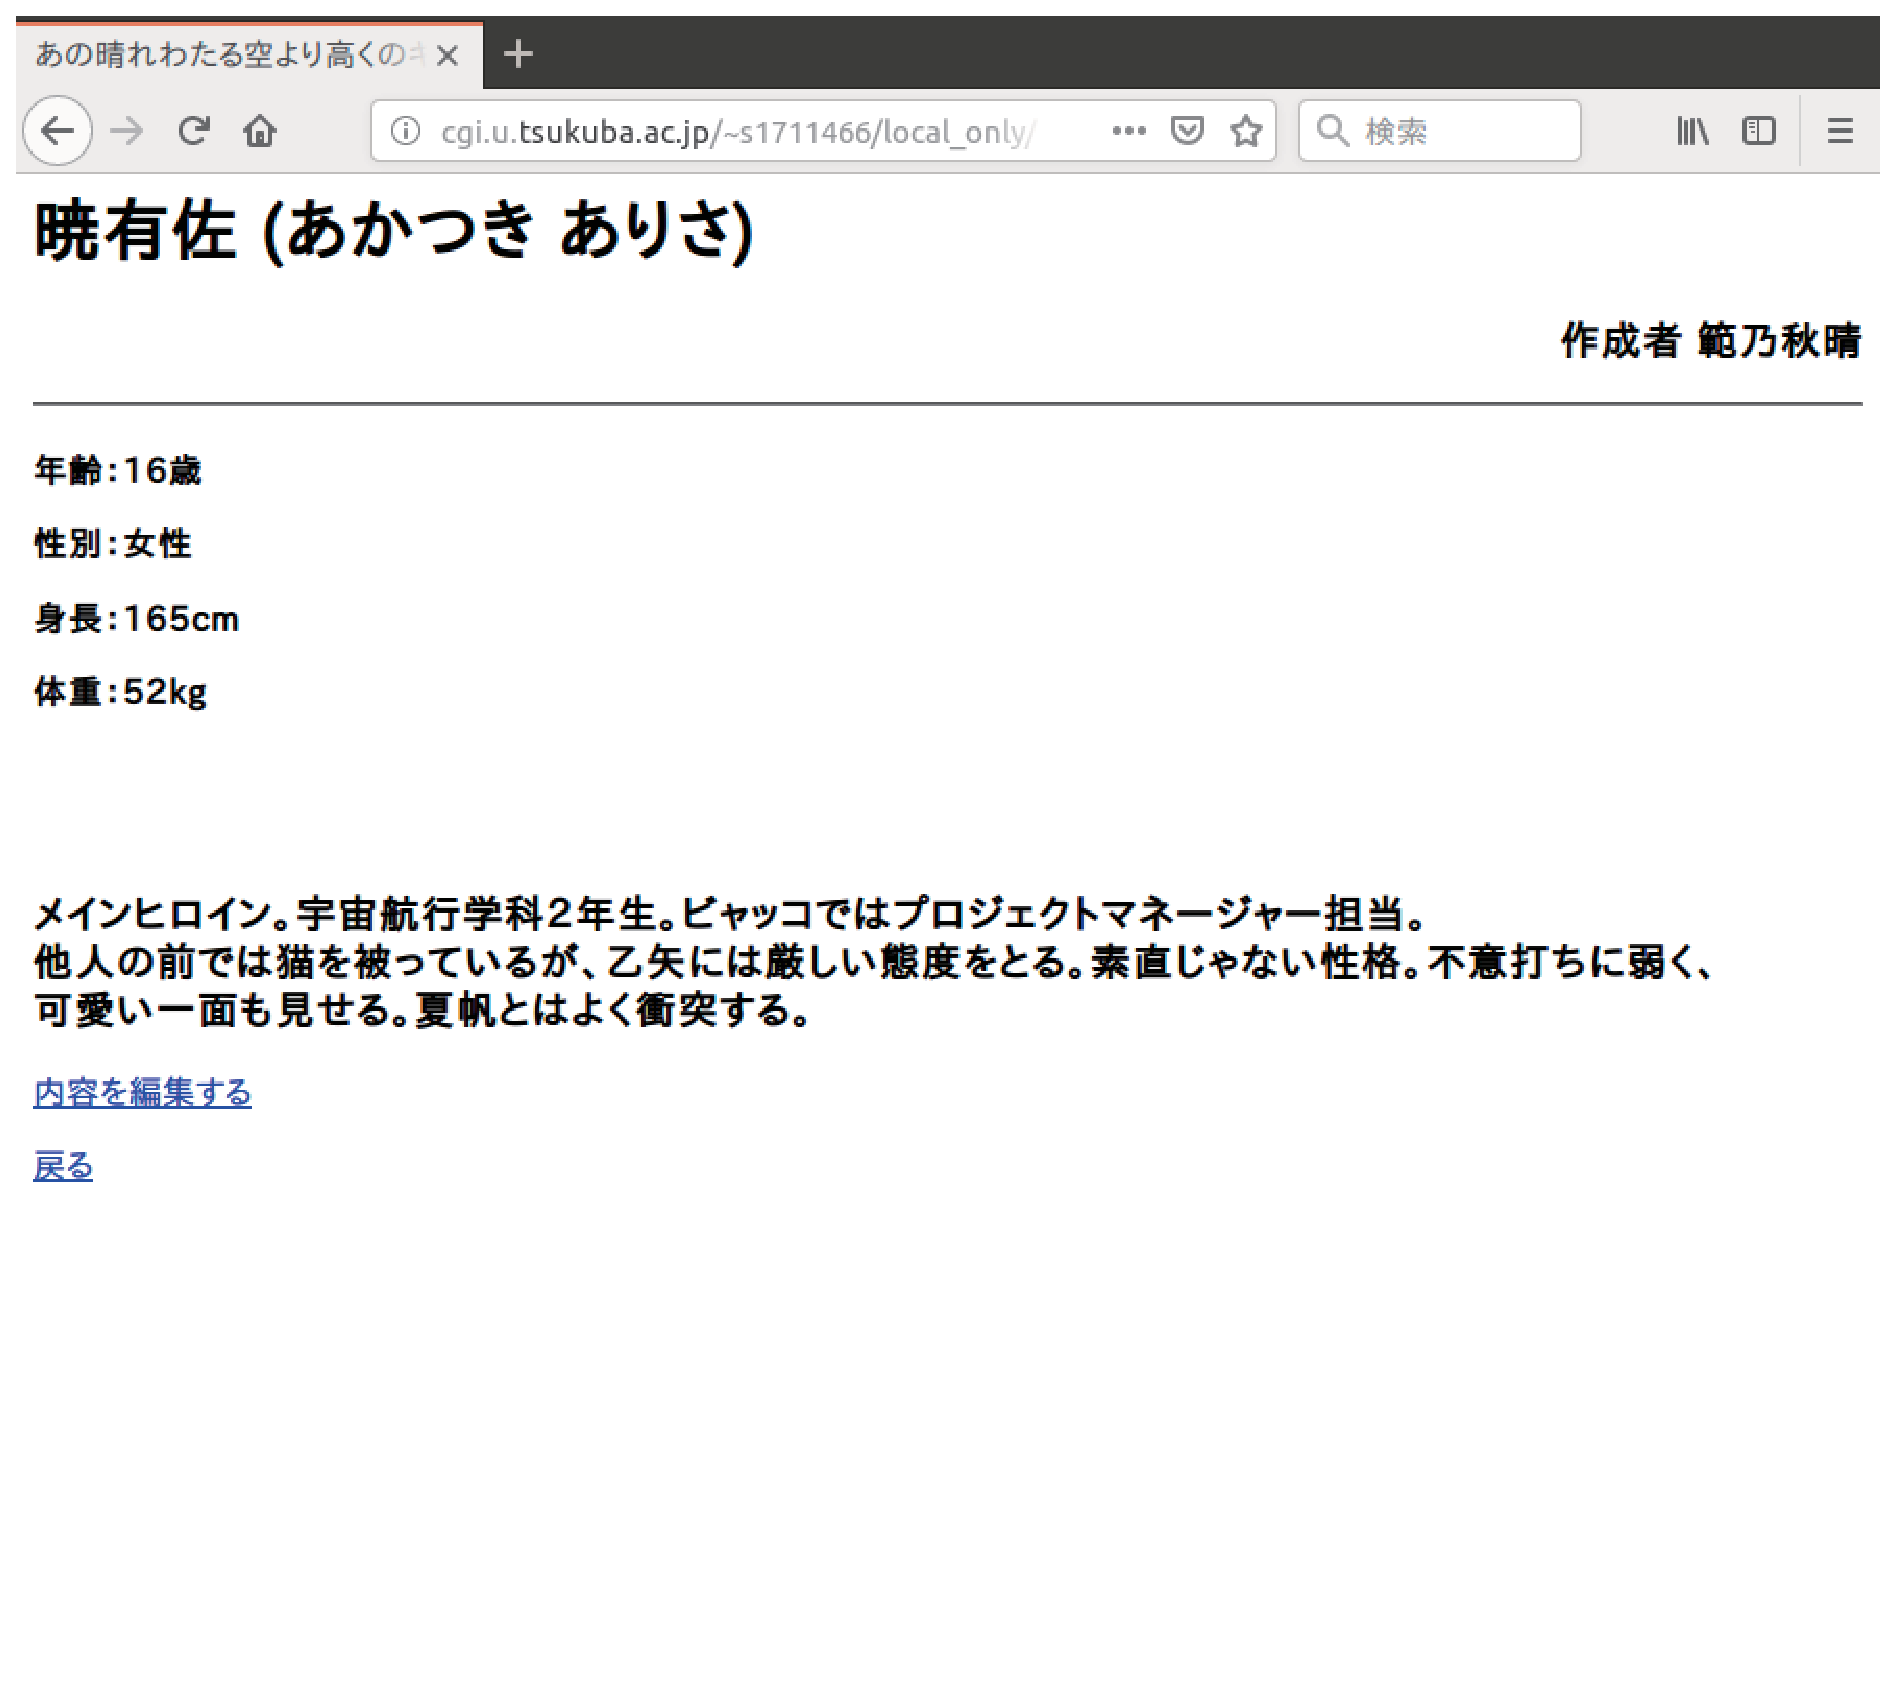
\includegraphics[width=7.0cm]{10-3-30.eps}
          \hspace{1.6cm} [1]キャラクターの個別ページ
        \end{center}
      \end{minipage}

      % 2 
      \begin{minipage}{0.55\hsize}
        \begin{center}
          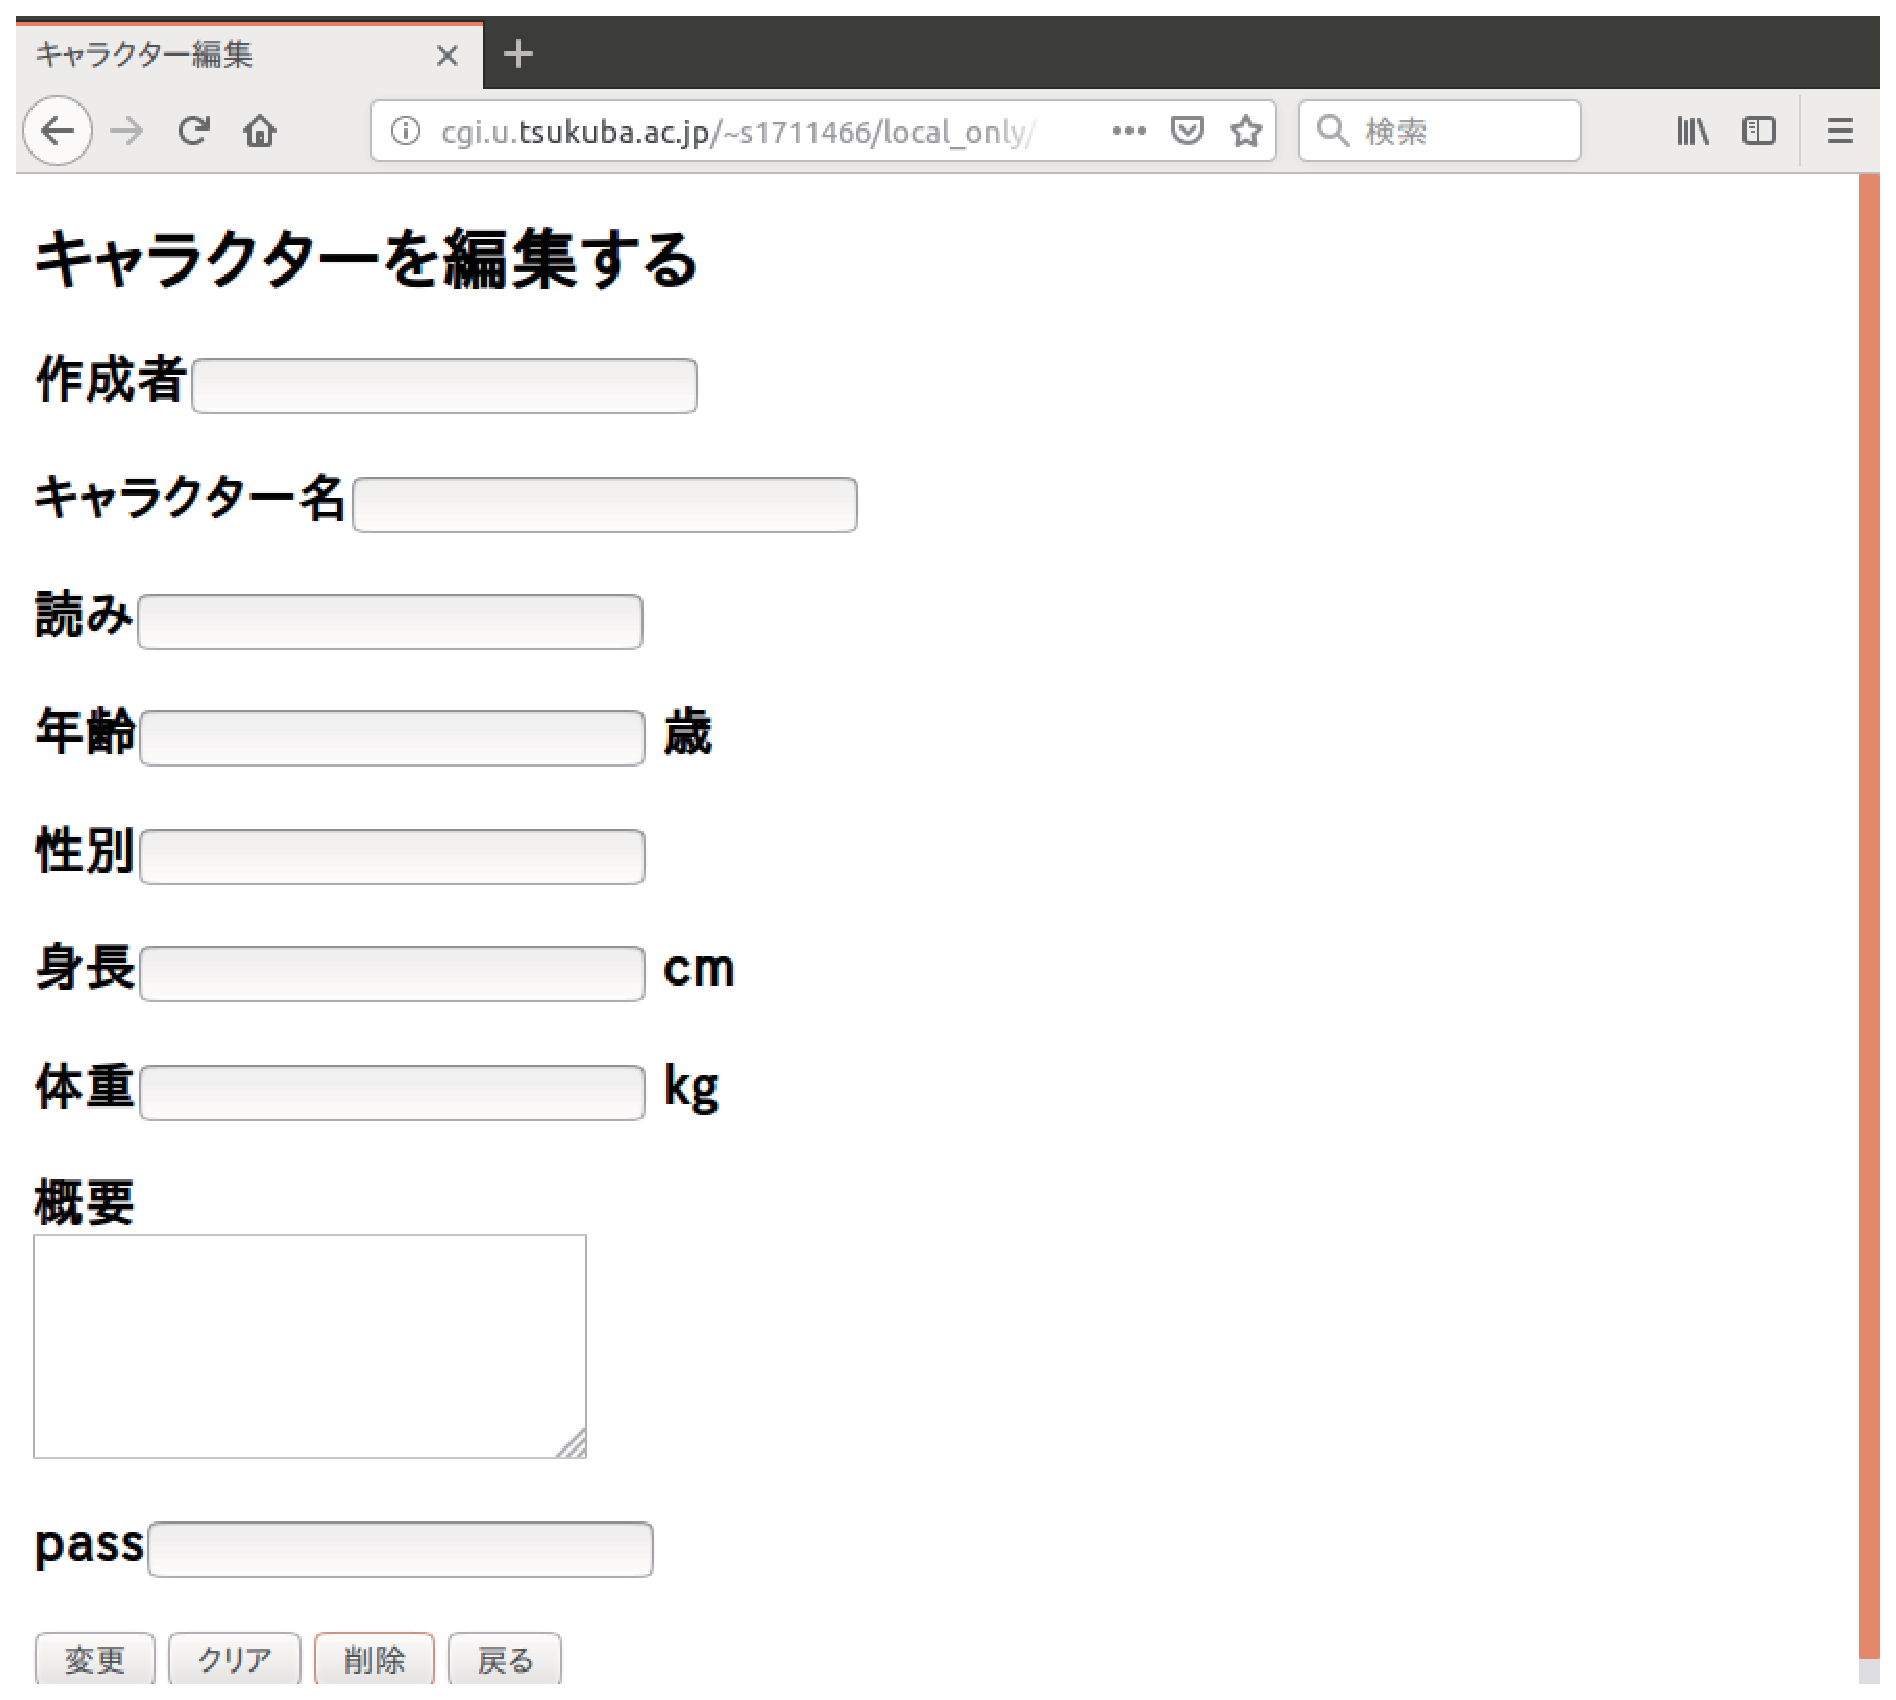
\includegraphics[width=6.7cm]{10-3-31.eps}
          \hspace{1.6cm} [2]キャラクターを削除する
        \end{center}
      \end{minipage}

      \begin{minipage}{0.55\hsize}
        \vspace{30mm}
      \end{minipage} \\
 
      % 3
      \begin{minipage}{0.5\hsize}
        \begin{center}
          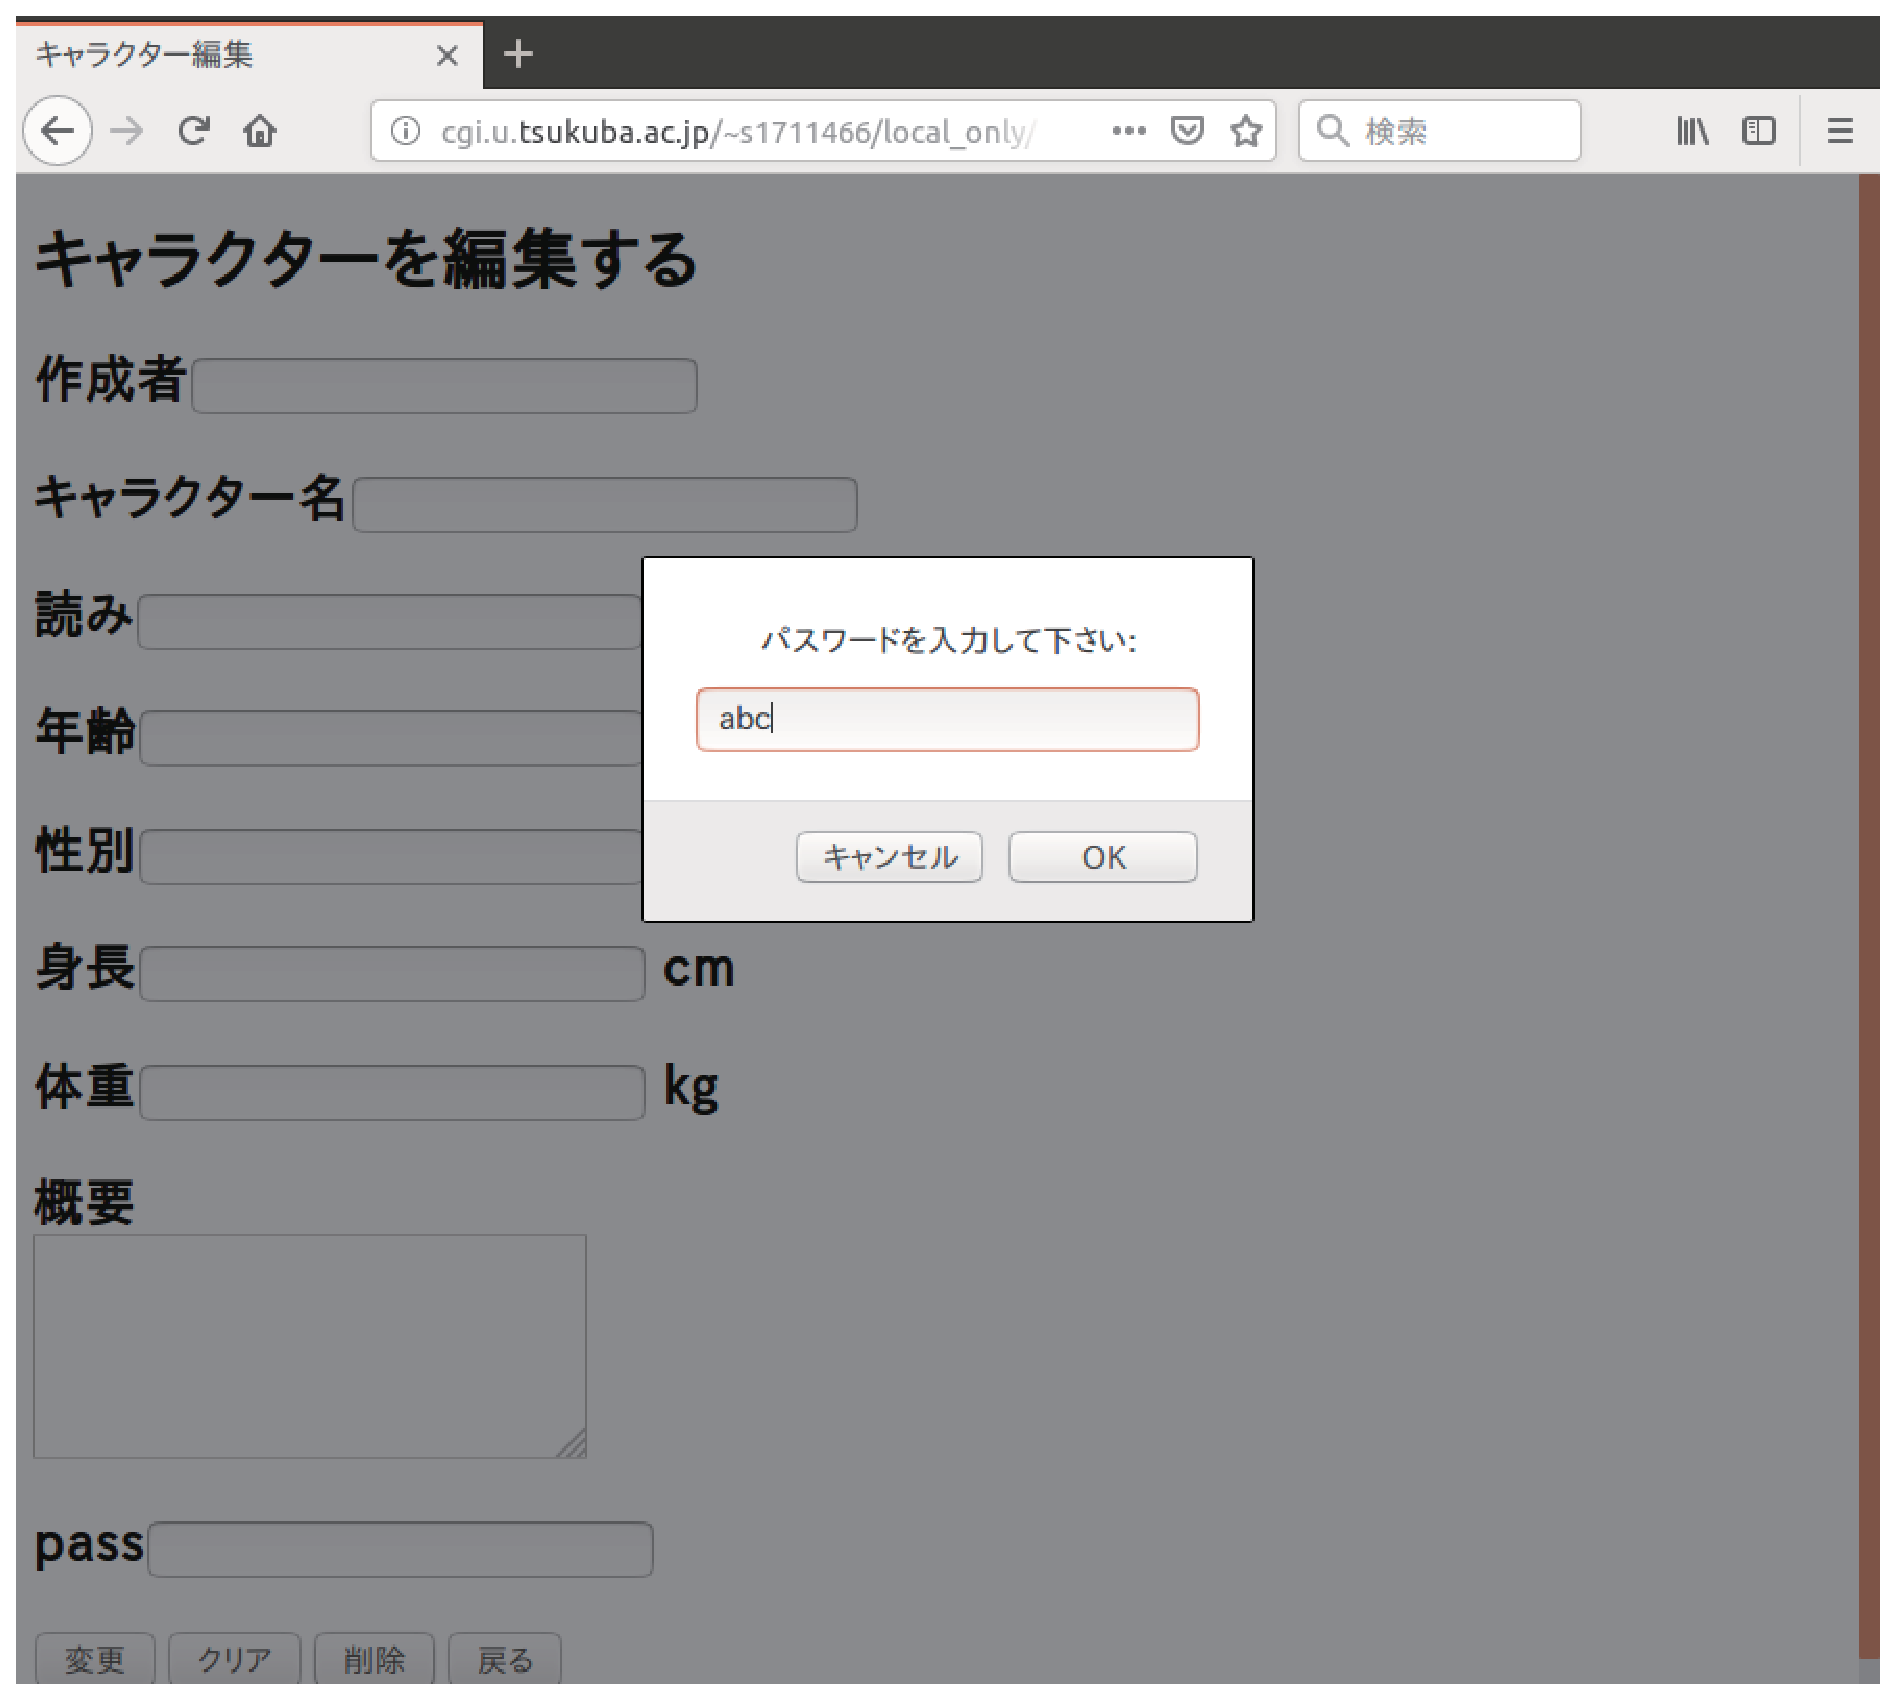
\includegraphics[width=6.7cm]{10-3-32.eps}
          \hspace{1.6cm} [3]パスワード要求
        \end{center}
      \end{minipage}

      % 4
      \begin{minipage}{0.55\hsize}
        \begin{center}
          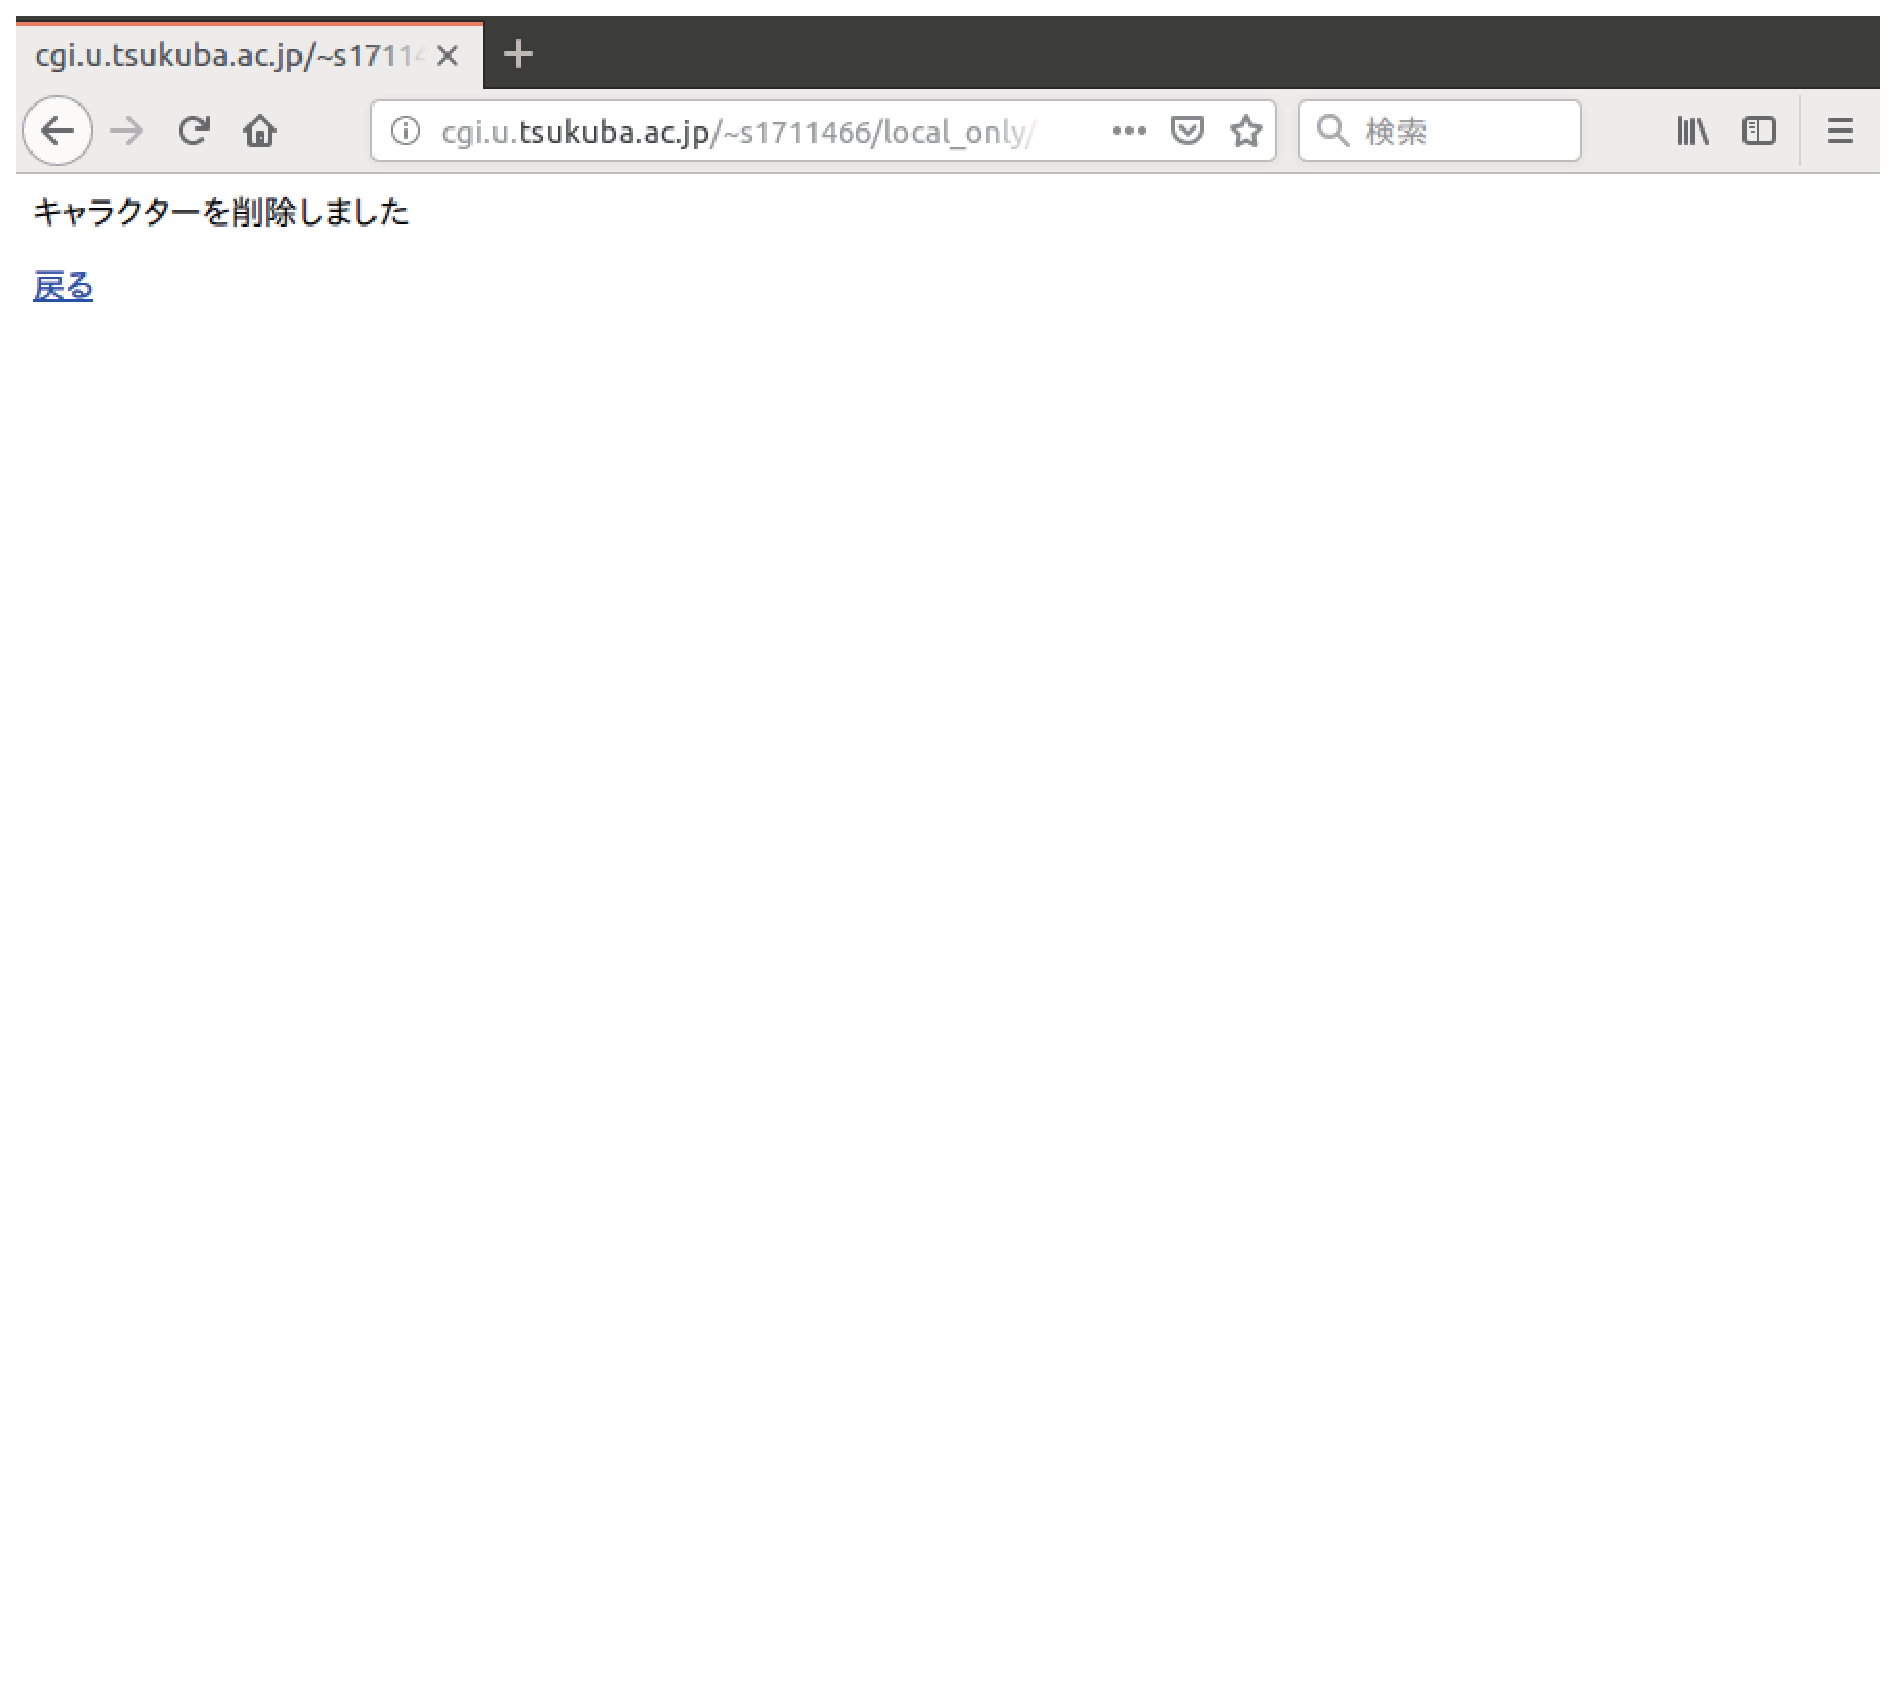
\includegraphics[width=6.7cm]{10-3-33.eps}
          \hspace{1.6cm} [4]削除完了
        \end{center}
      \end{minipage}

      \begin{minipage}{0.55\hsize}
        \vspace{90mm}
      \end{minipage} \\

      % 5
      \begin{minipage}{0.55\hsize}
        \begin{center}
          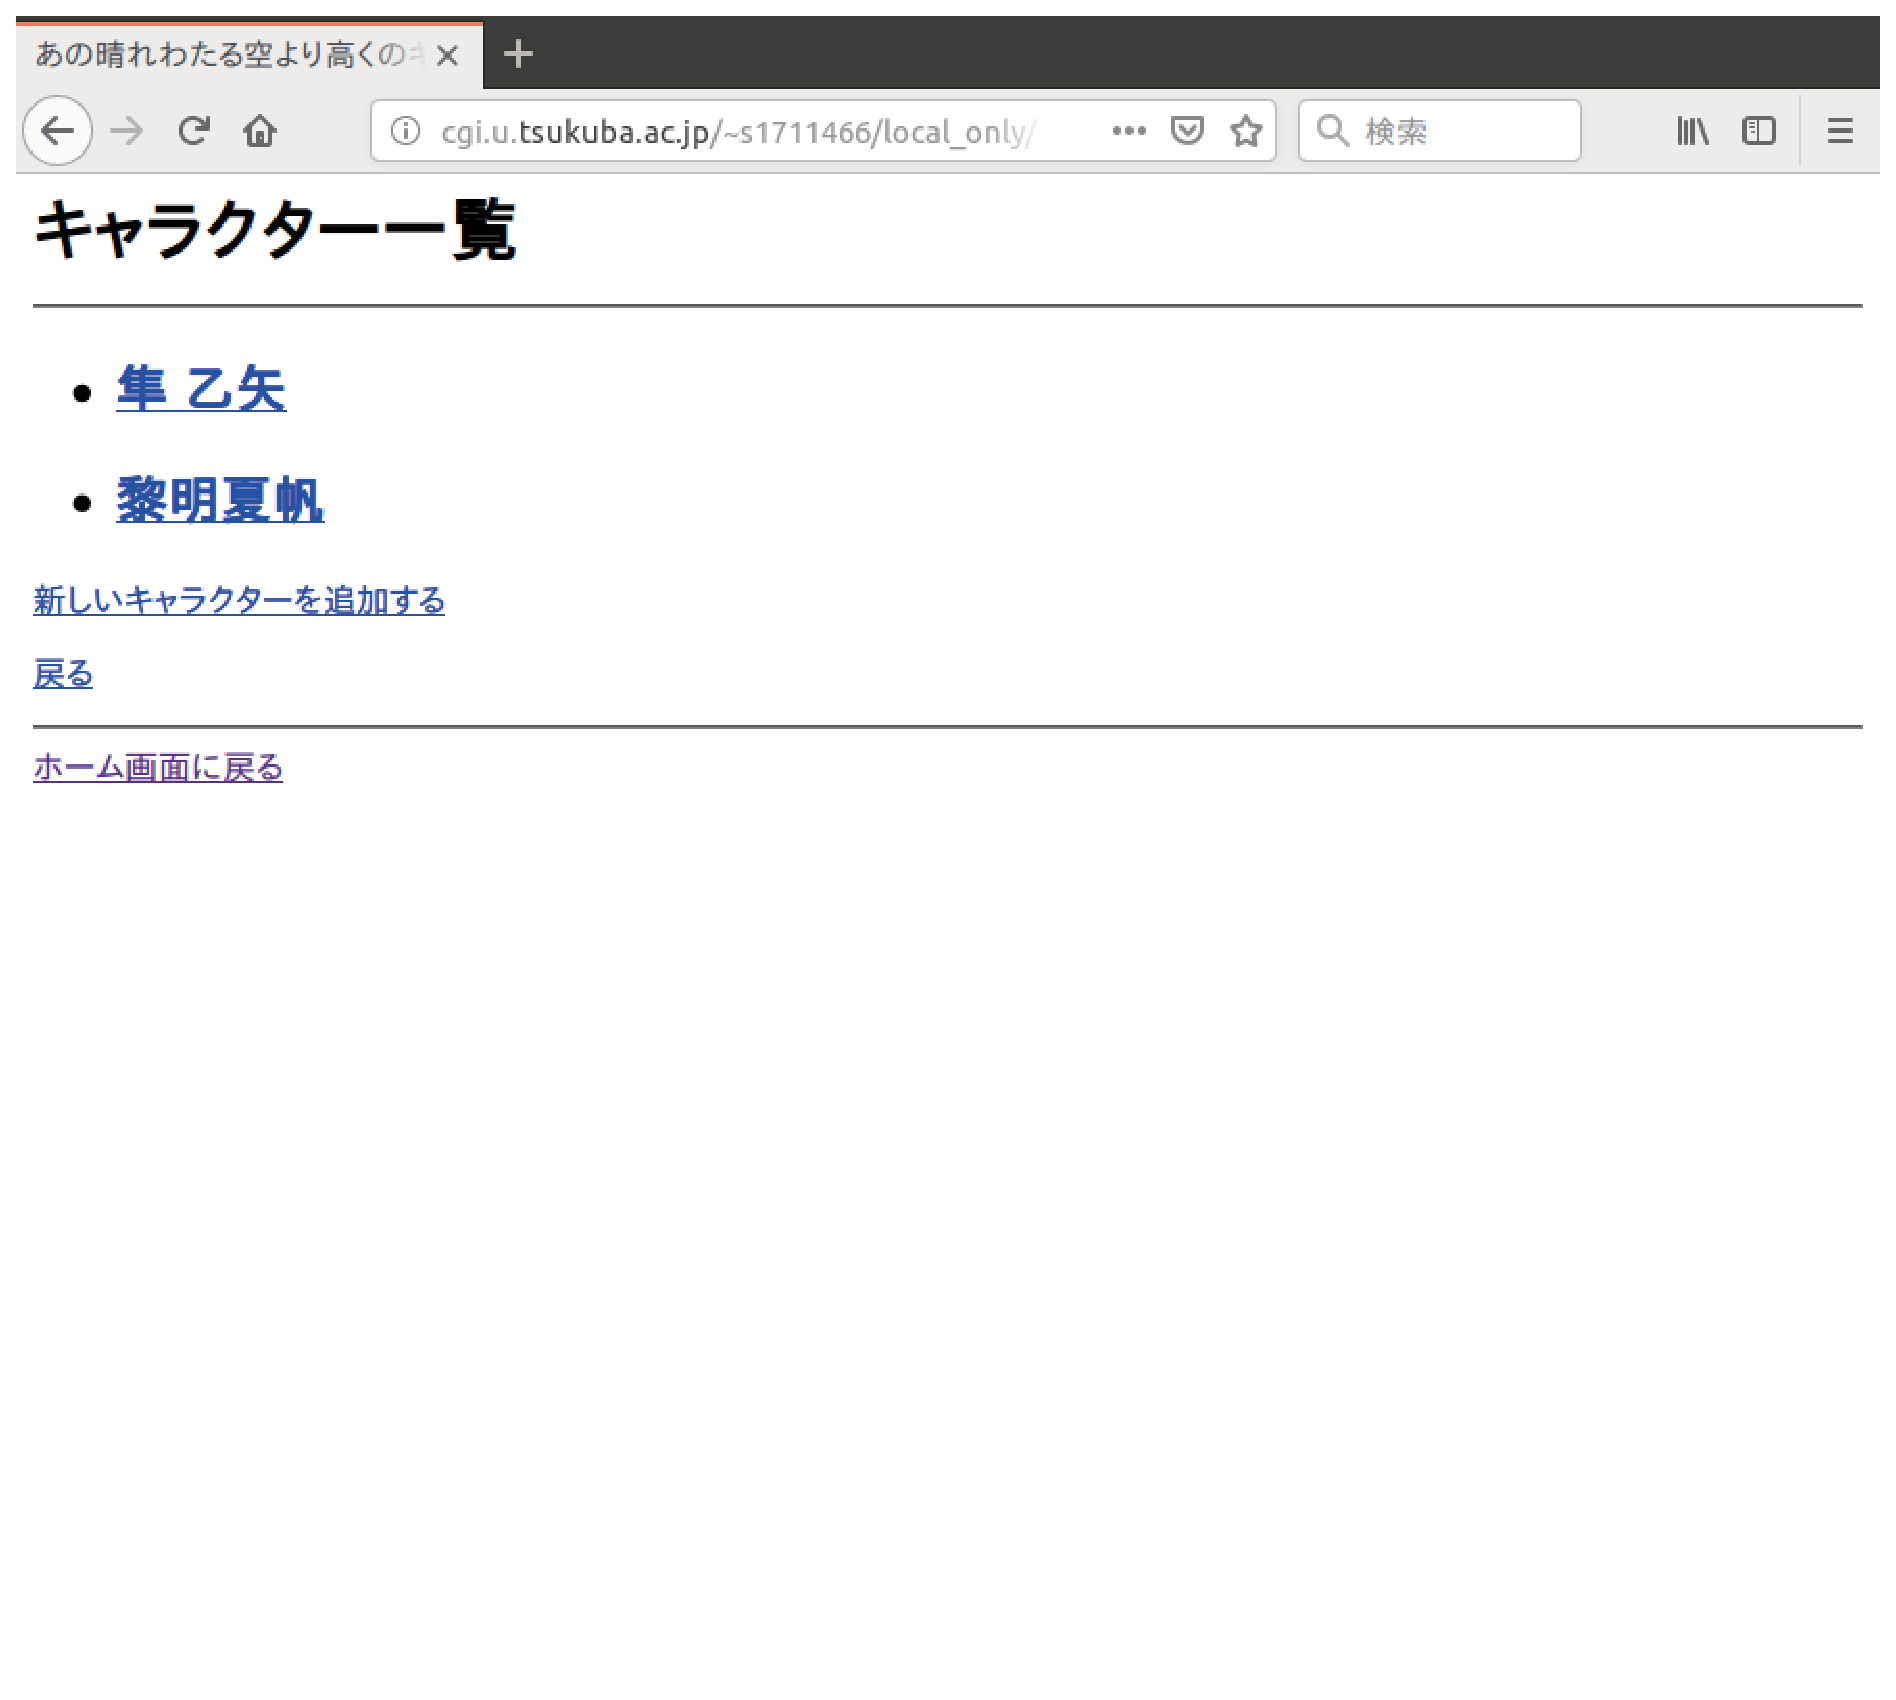
\includegraphics[width=6.7cm]{10-3-34.eps}
          \hspace{1.6cm} [5]内容削除後のキャラクター一覧のページ
        \end{center}
      \end{minipage}

    \end{tabular}
    \caption{用語の削除関係の動作画面}
    \label{fig:b}
  \end{center}
\end{figure}

\begin{figure}[htbp]
  \begin{center}
    \begin{tabular}{c}

      % 1 ホーム画面
      \begin{minipage}{0.55\hsize}
        \begin{center}
          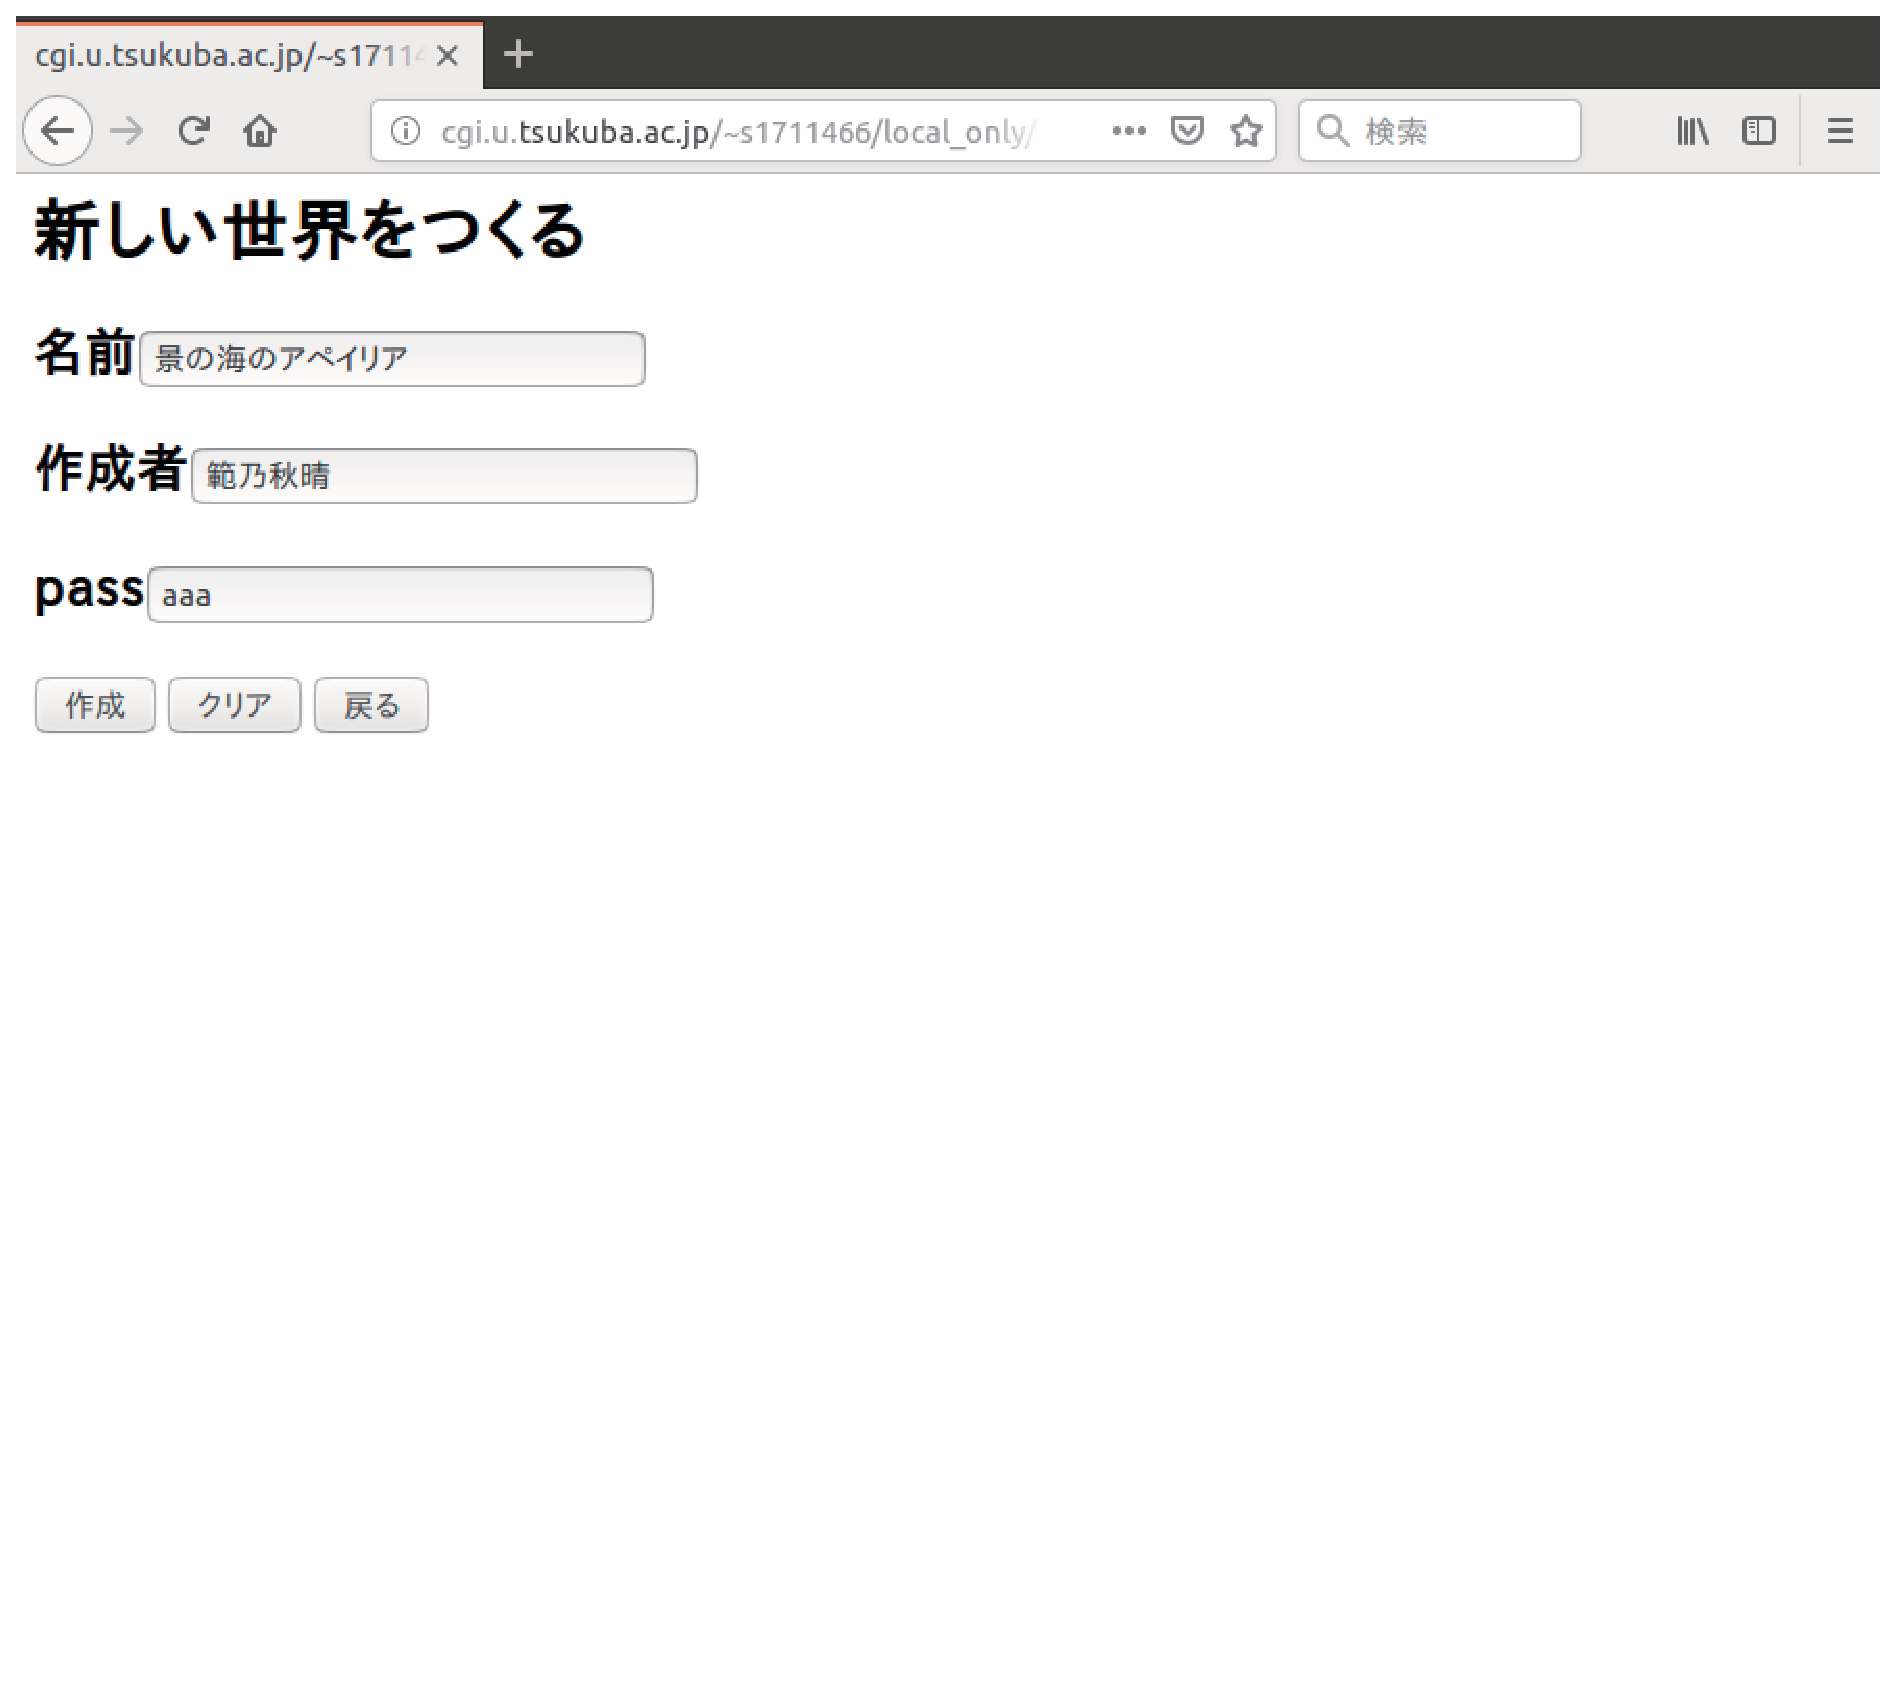
\includegraphics[width=7.0cm]{10-3-37.eps}
          \hspace{1.6cm} [1]既存と同名(景の海のアペイリア)の世界をつくろうとする
        \end{center}
      \end{minipage}

      % 2 
      \begin{minipage}{0.55\hsize}
        \begin{center}
          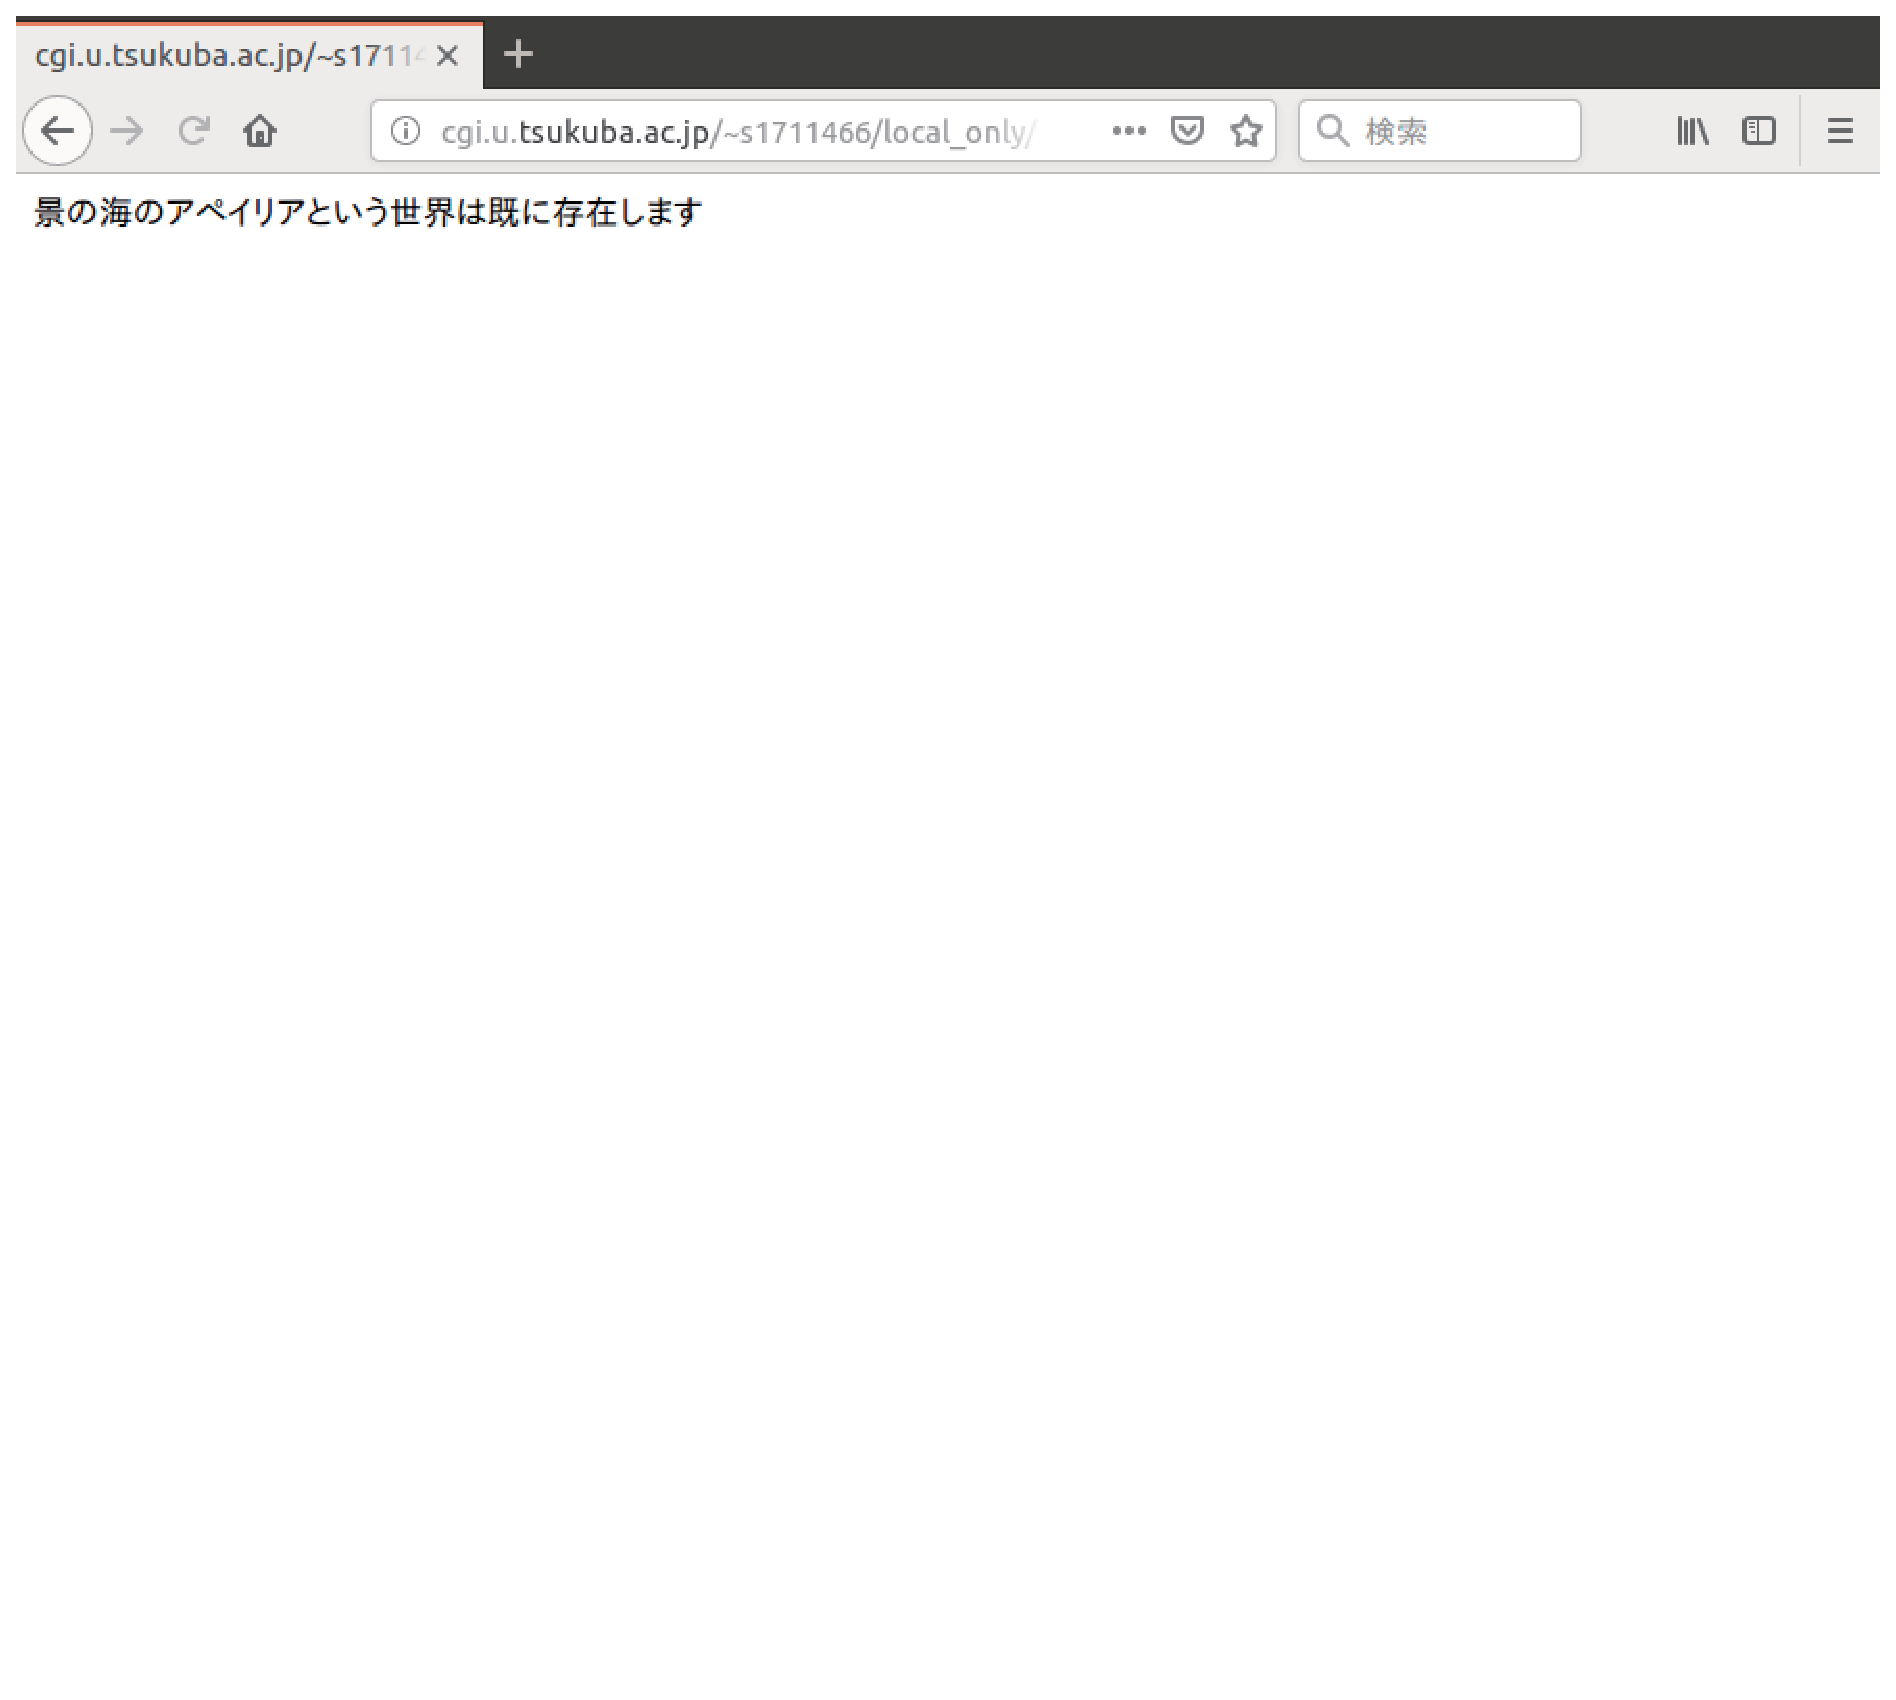
\includegraphics[width=6.7cm]{10-3-38.eps}
          \hspace{1.6cm} [2]エラーメッセージ
        \end{center}
      \end{minipage}

      \begin{minipage}{0.55\hsize}
        \vspace{90mm}
      \end{minipage} \\
 
      % 3
      \begin{minipage}{0.5\hsize}
        \begin{center}
          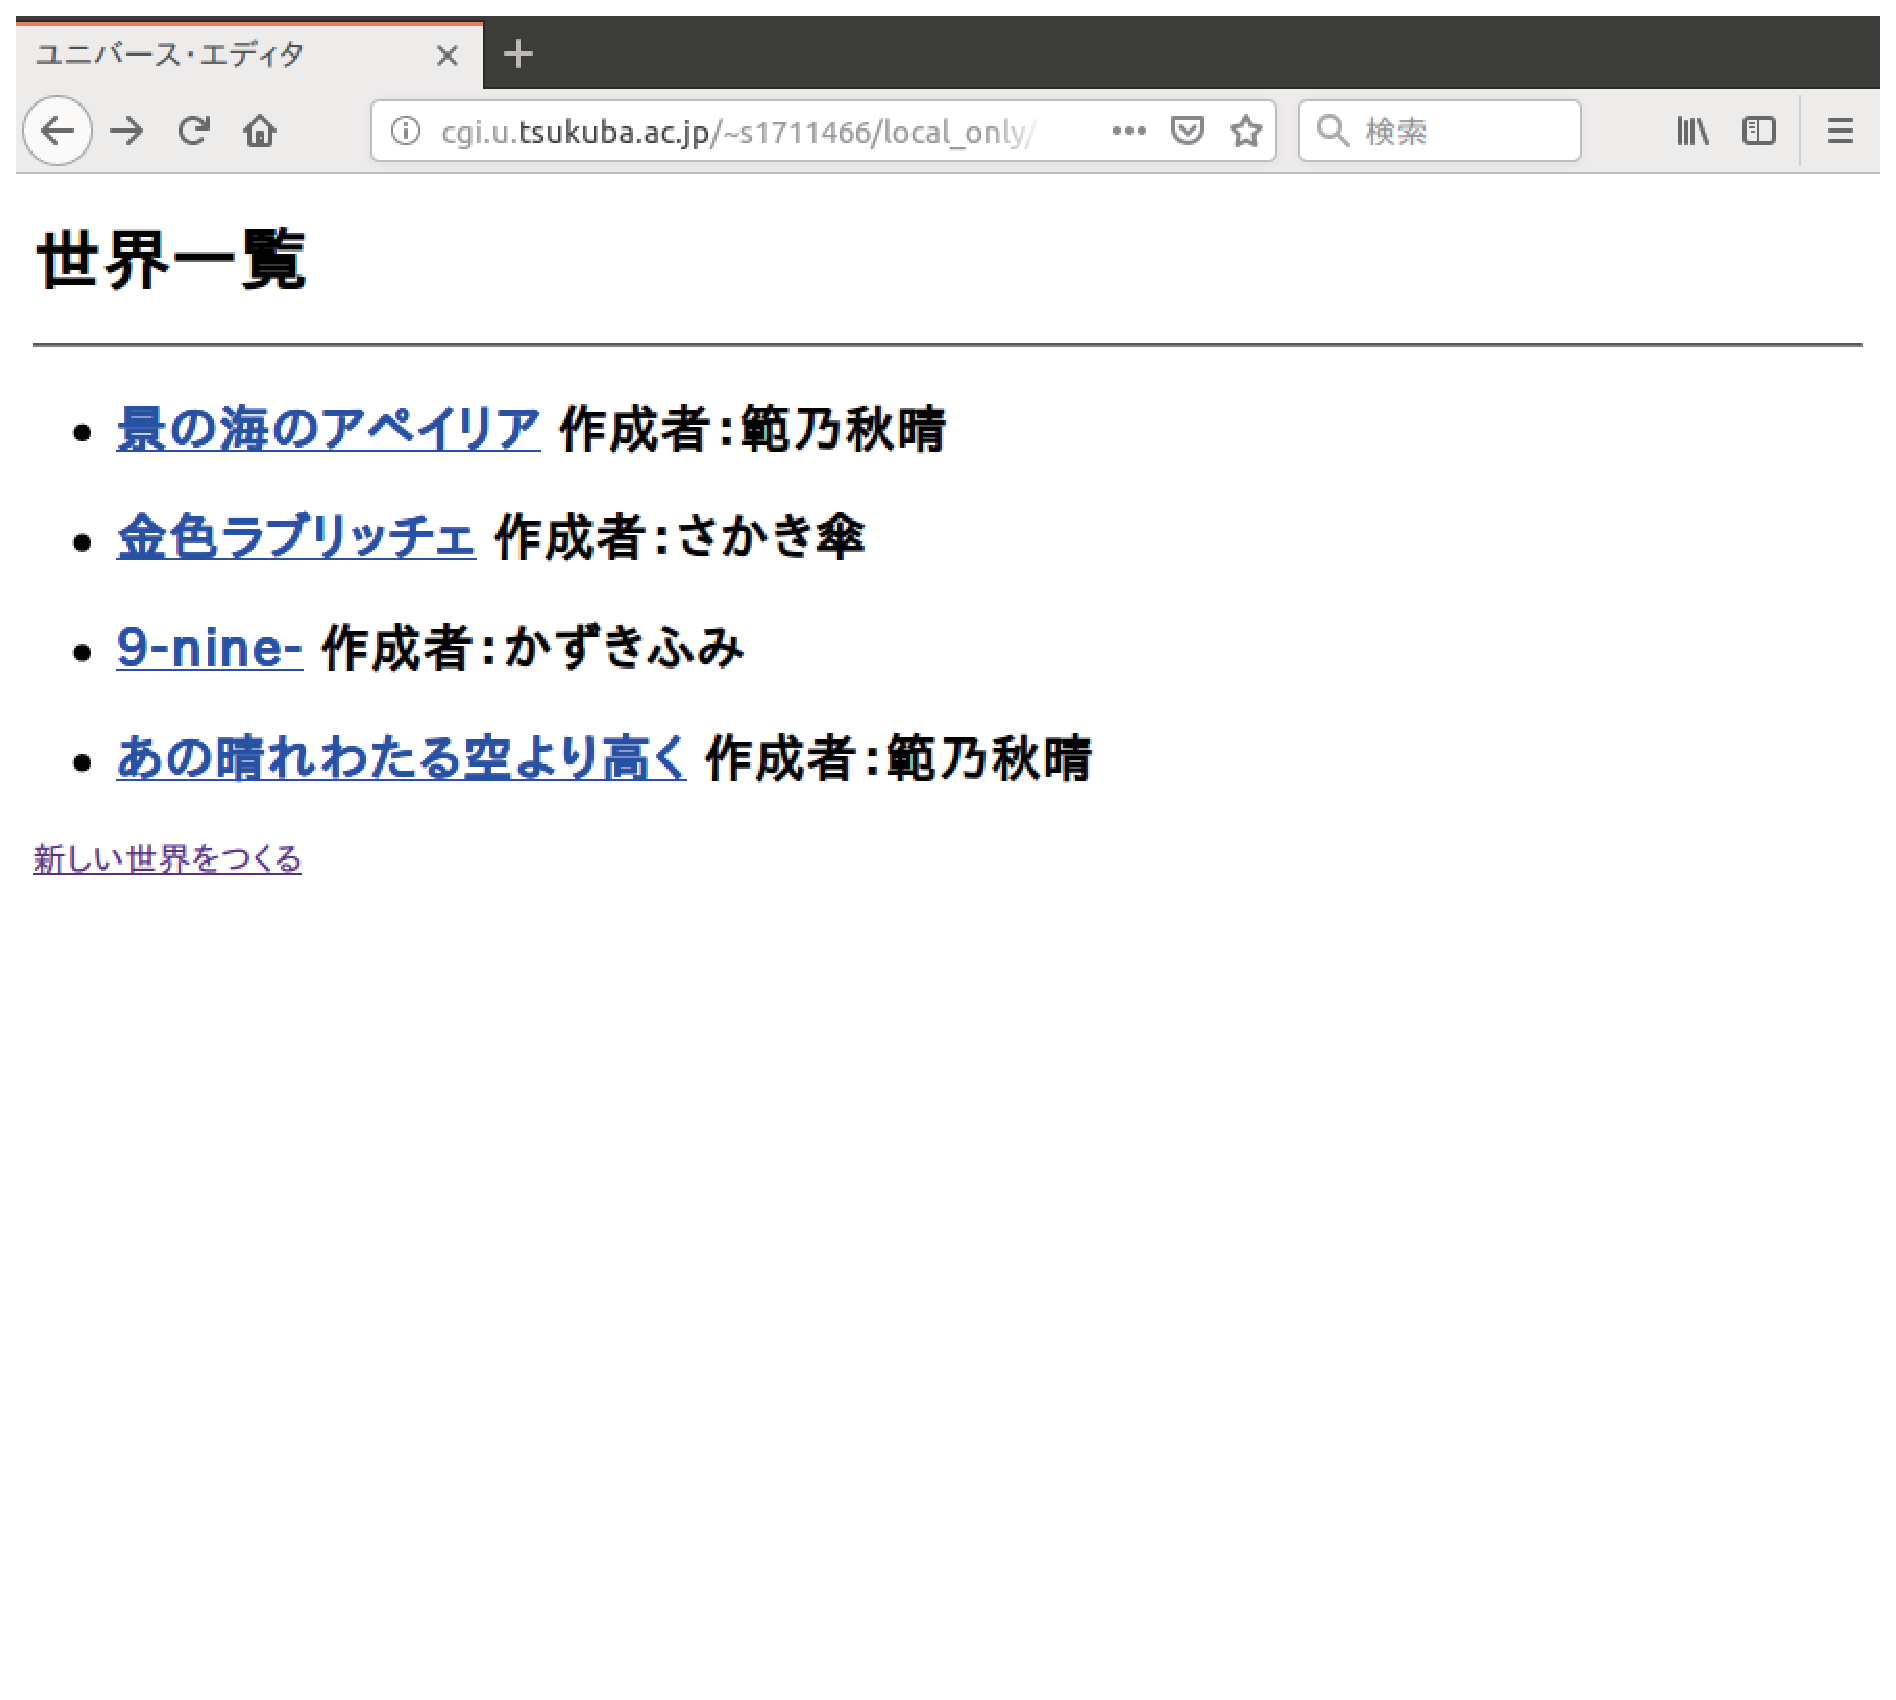
\includegraphics[width=6.7cm]{10-3-39.eps}
          \hspace{1.6cm} [3]ホーム画面
        \end{center}
      \end{minipage}

    \end{tabular}
    \caption{同名の世界を作成しようとした場合の動作画面}
    \label{fig:b}
  \end{center}
\end{figure}

\begin{figure}[htbp]
  \begin{center}
    \begin{tabular}{c}

      % 1 ホーム画面
      \begin{minipage}{0.55\hsize}
        \begin{center}
          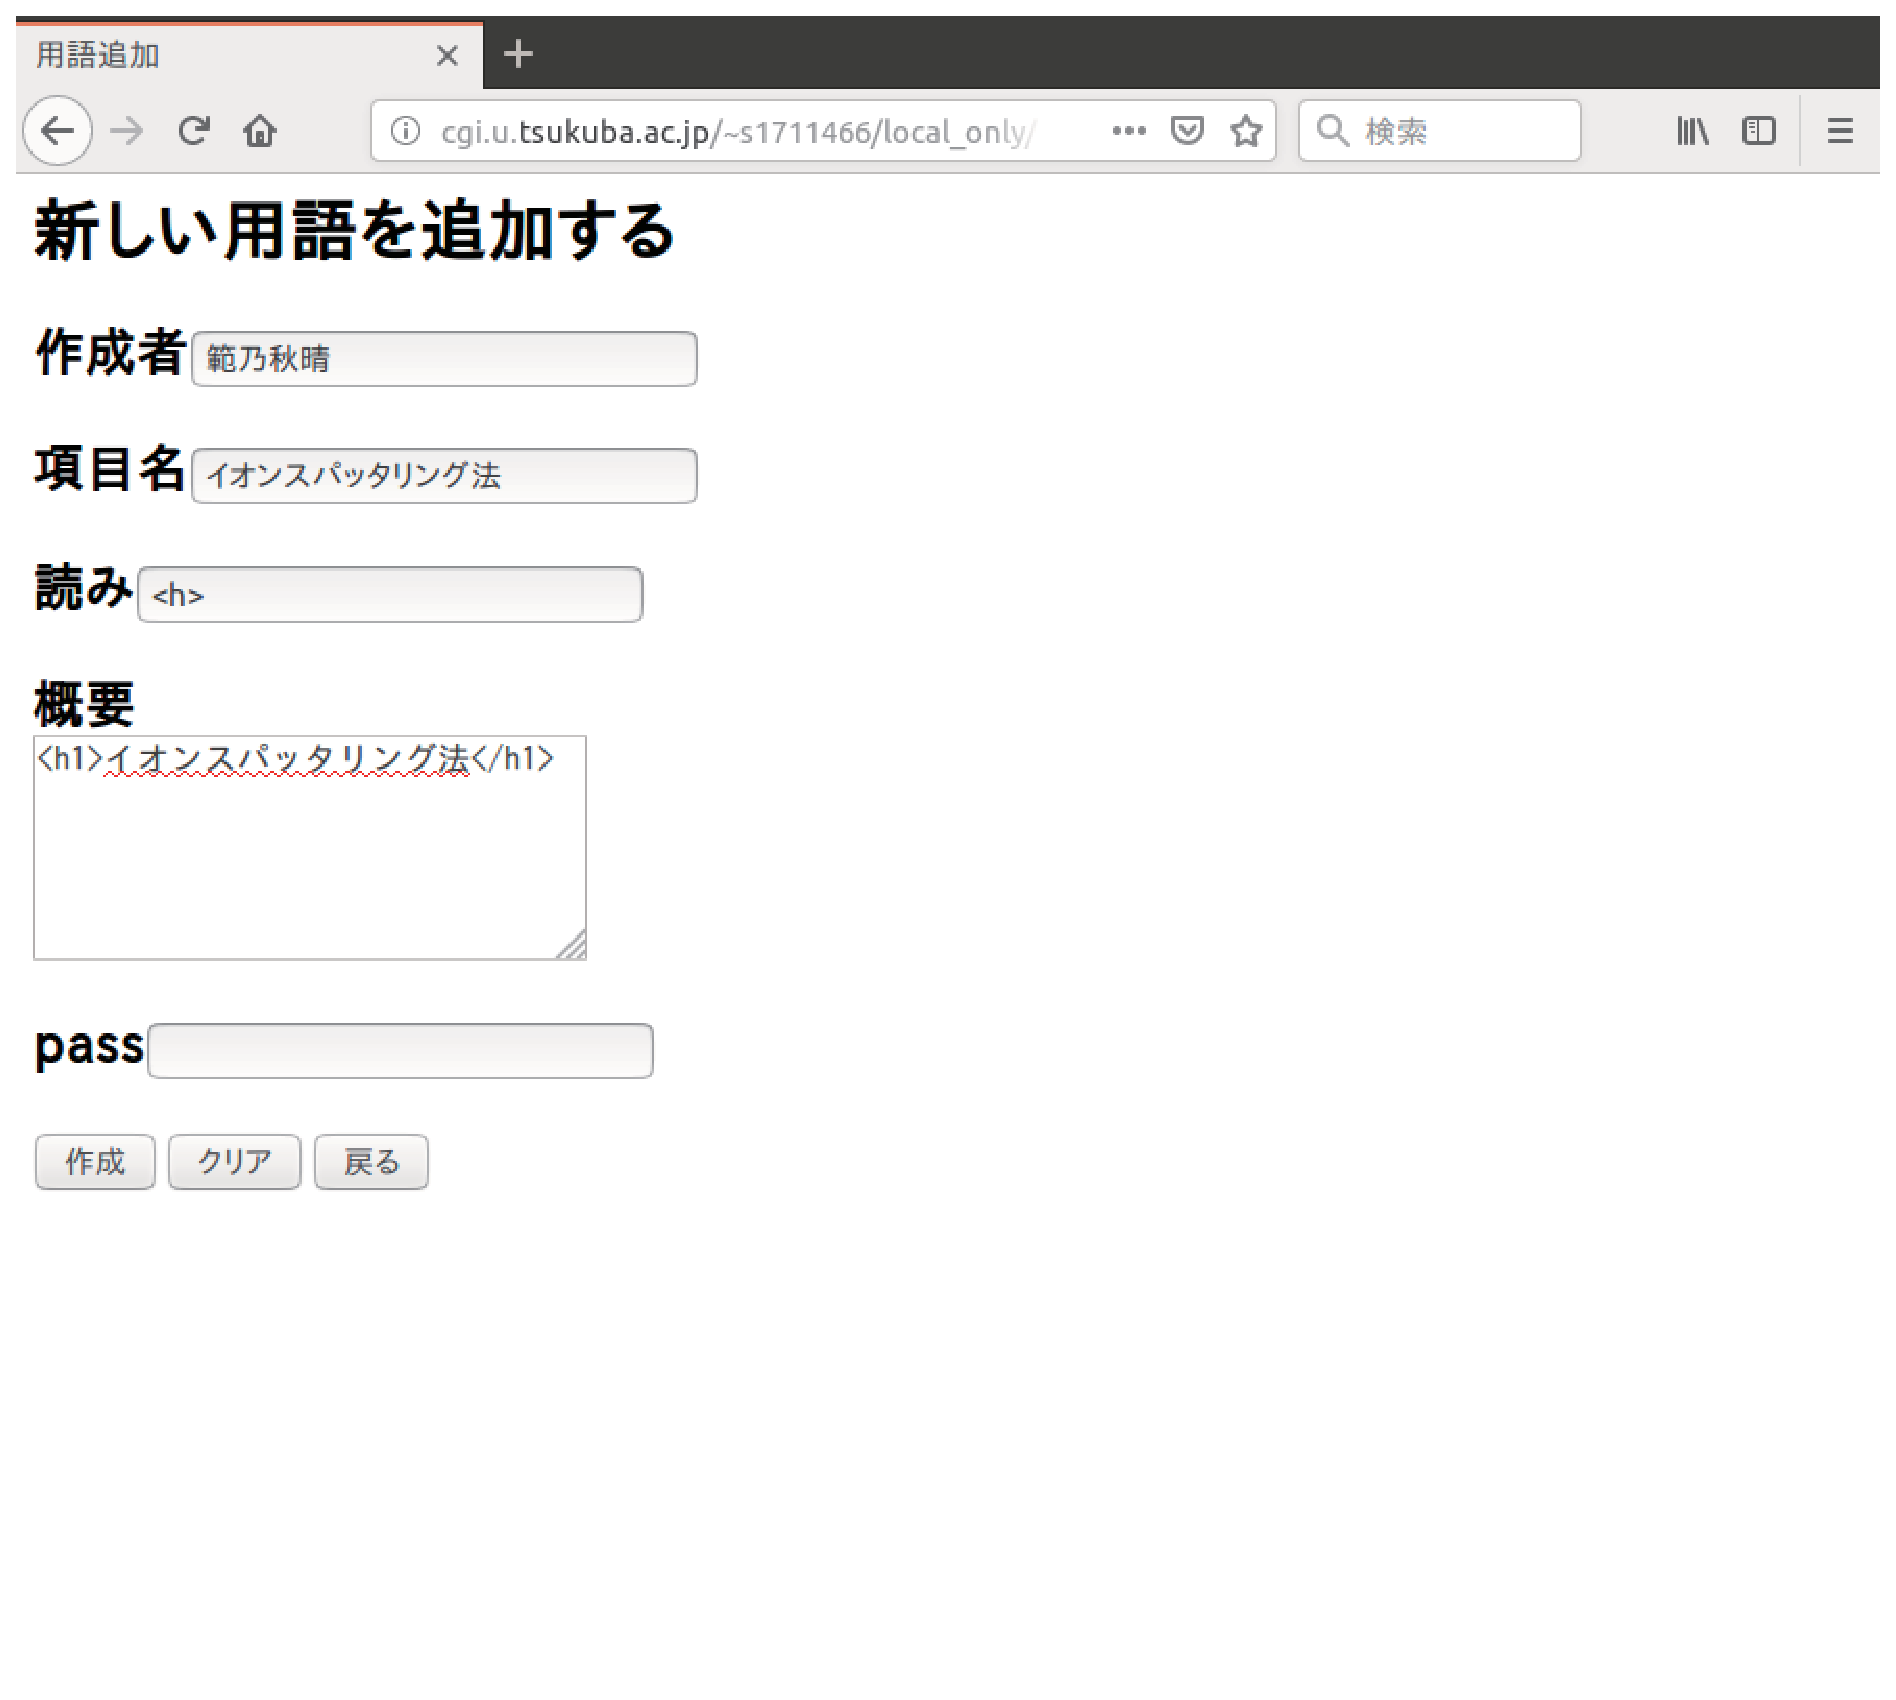
\includegraphics[width=7.0cm]{10-3-35.eps}
          \hspace{1.6cm} [1]HTMLのヘッダを入れようとする
        \end{center}
      \end{minipage}

      % 2 
      \begin{minipage}{0.55\hsize}
        \begin{center}
          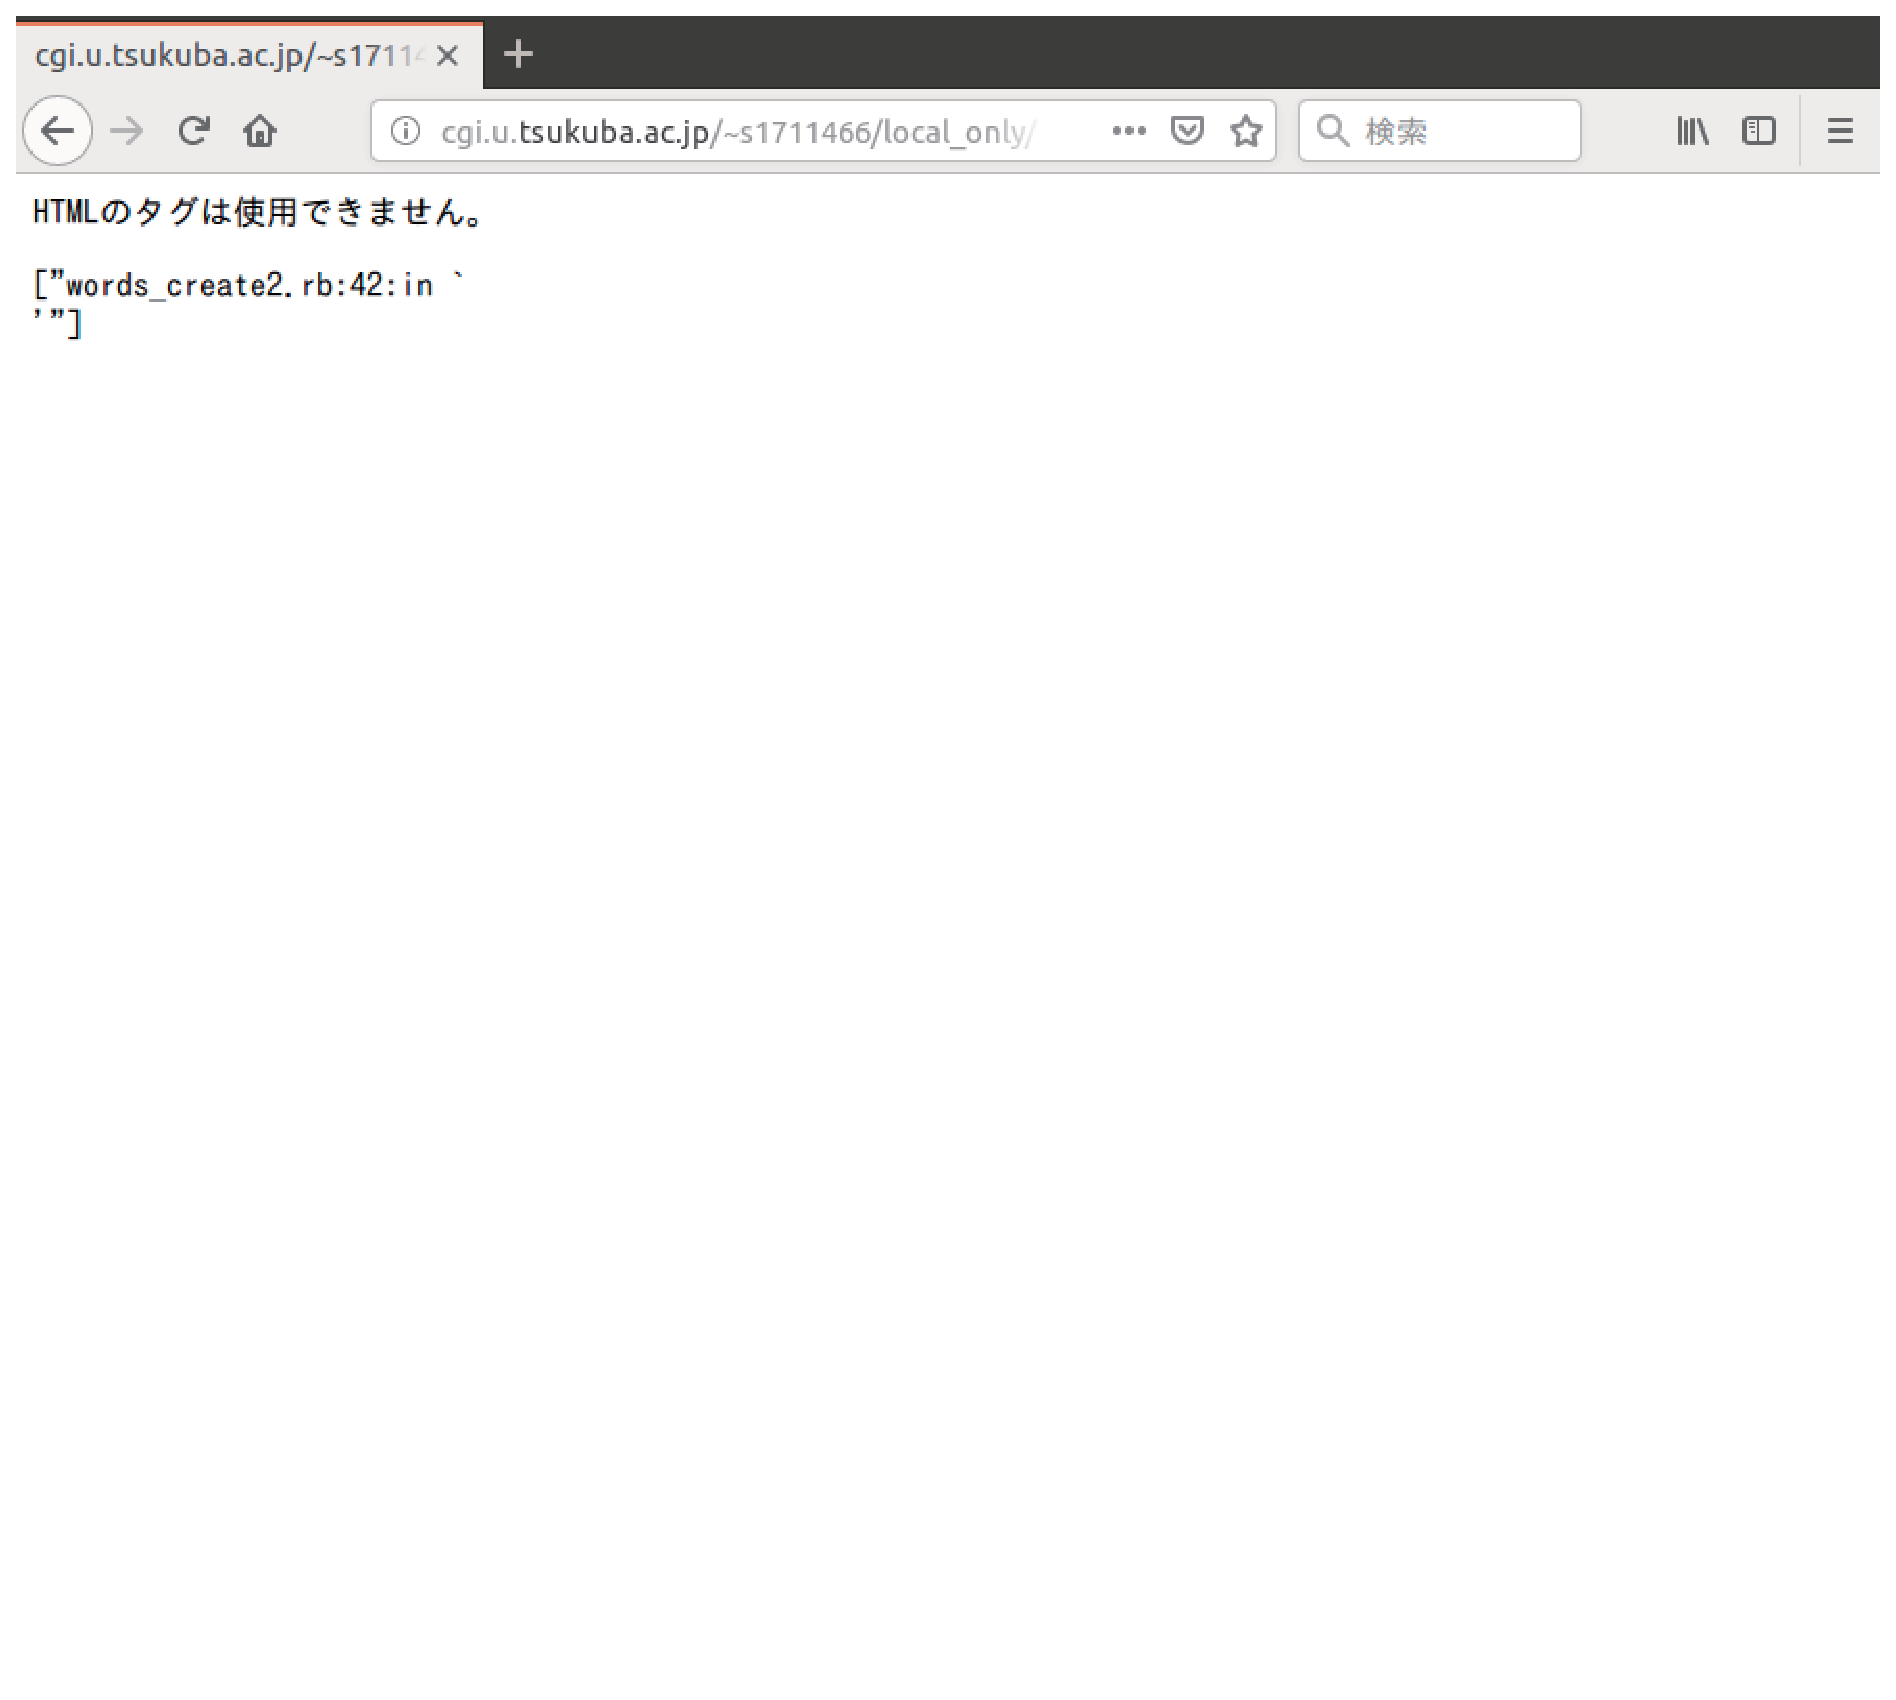
\includegraphics[width=6.7cm]{10-3-36.eps}
          \hspace{1.6cm} [2]エラーメッセージ
        \end{center}
      \end{minipage}

      \begin{minipage}{0.55\hsize}
        \vspace{90mm}
      \end{minipage} \\
 
      % 3
      \begin{minipage}{0.5\hsize}
        \begin{center}
          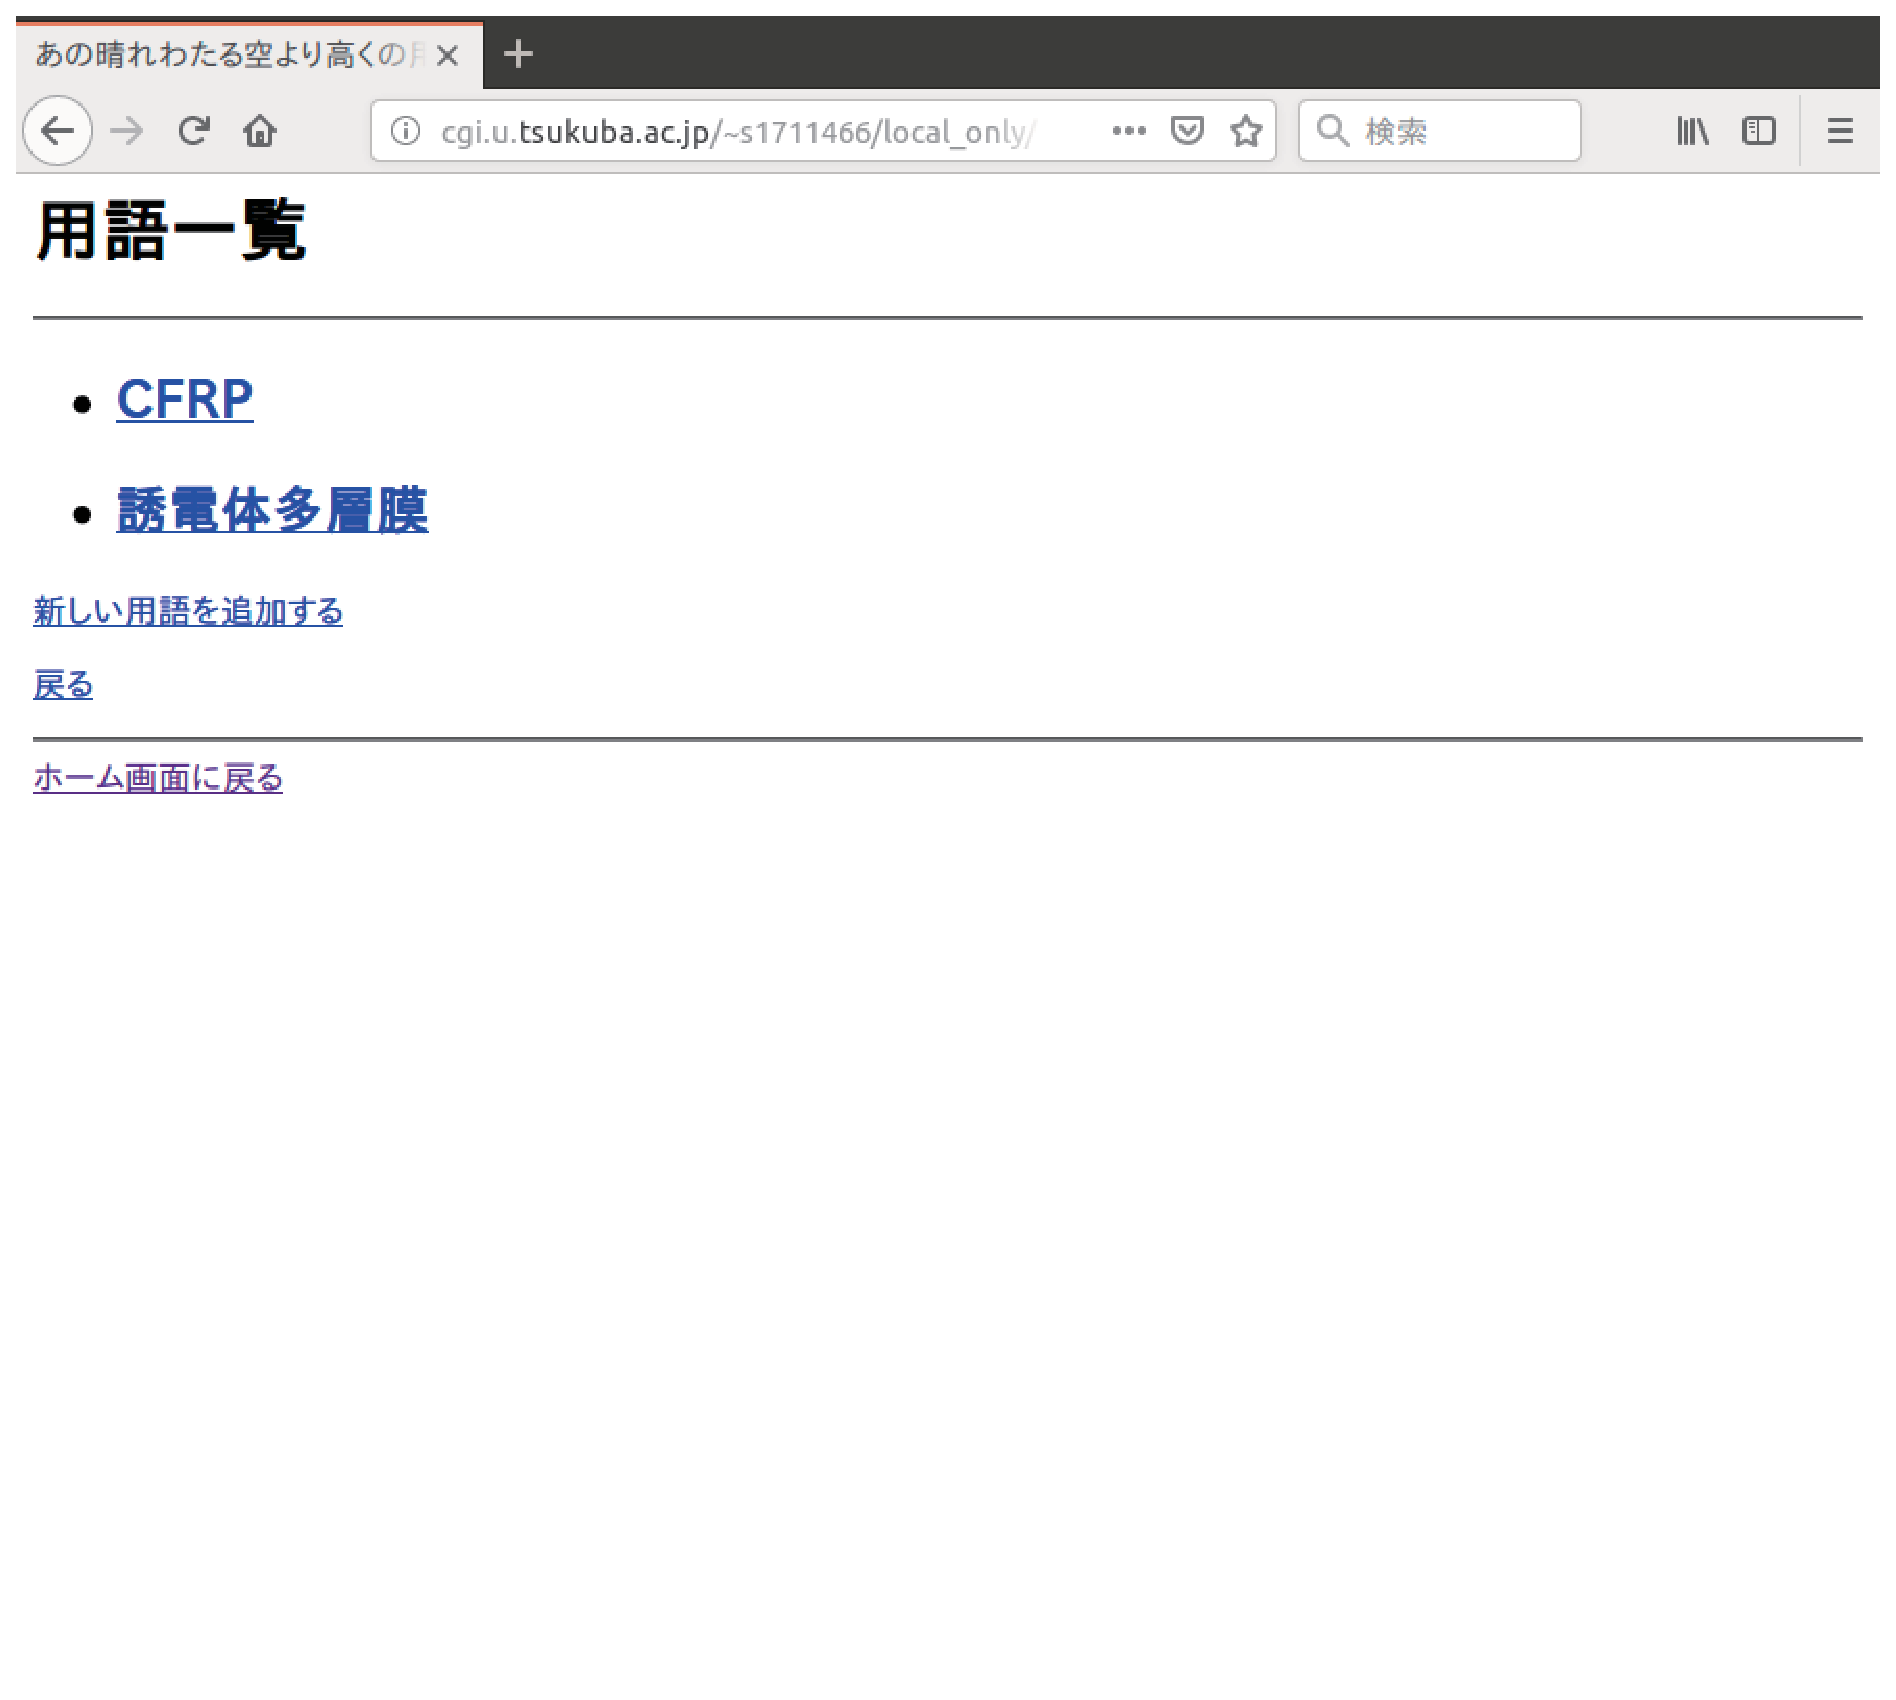
\includegraphics[width=6.7cm]{10-3-40.eps}
          \hspace{1.6cm} [3]用語一覧
        \end{center}
      \end{minipage}

    \end{tabular}
    \caption{HTMLヘッダを入力した場合の動作画面}
    \label{fig:b}
  \end{center}
\end{figure}

\begin{figure}[htbp]
  \begin{center}
    \begin{tabular}{c}

      % 1 ホーム画面
      \begin{minipage}{0.55\hsize}
        \begin{center}
          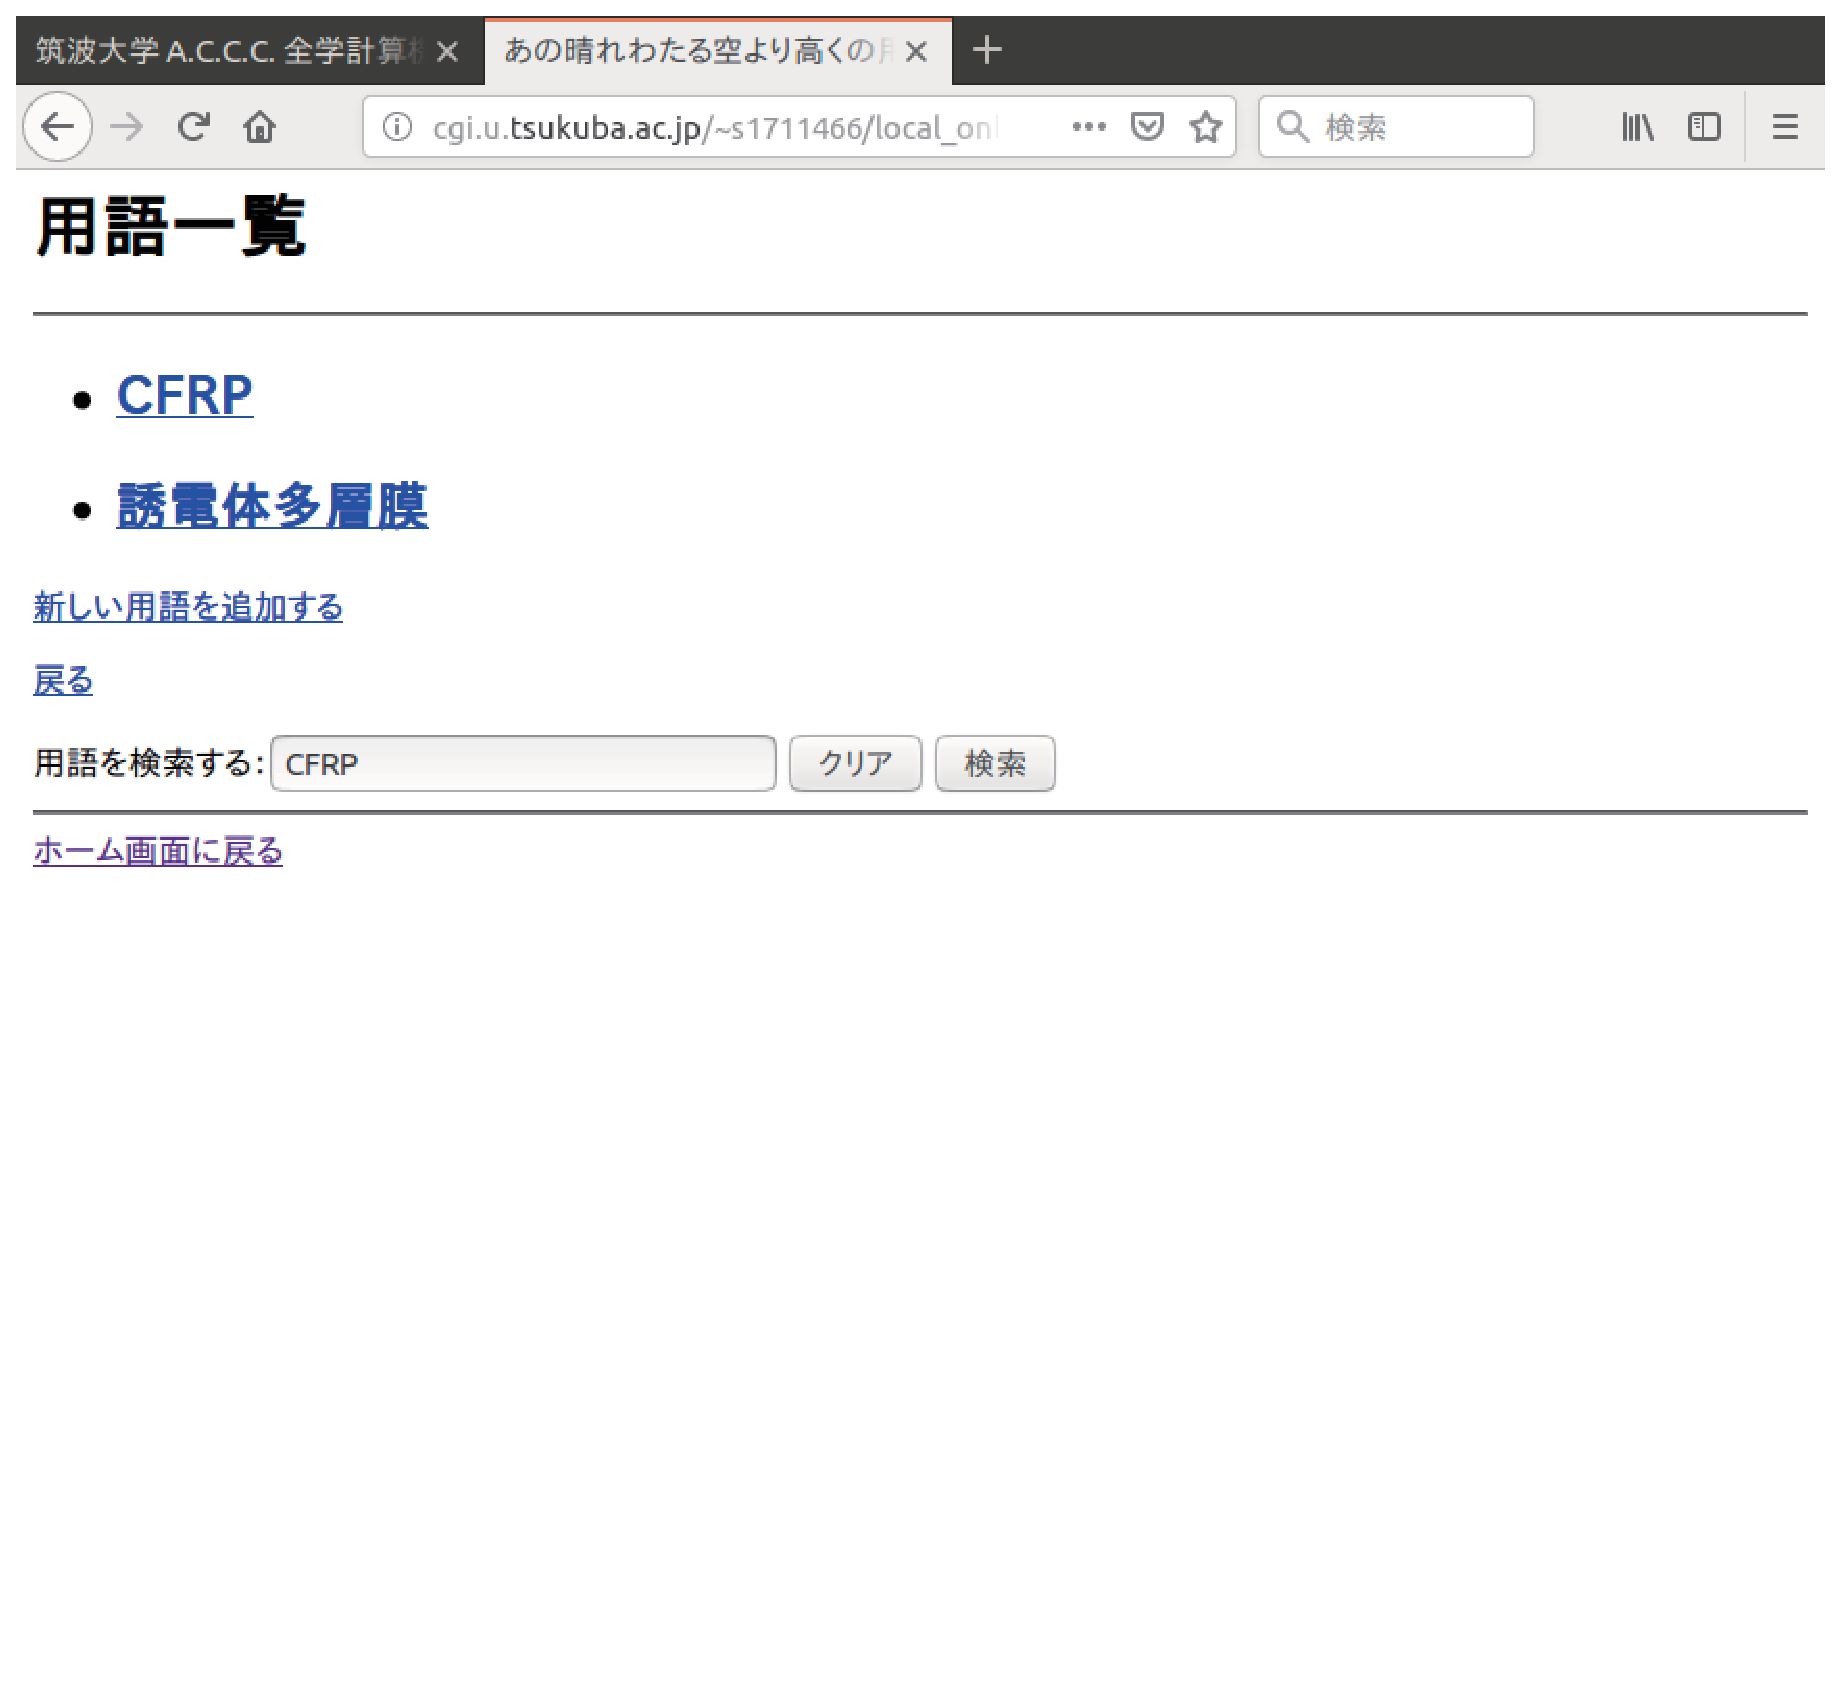
\includegraphics[width=7.0cm]{10-3-41.eps}
          \hspace{1.6cm} [1]用語を検索する
        \end{center}
      \end{minipage}

      % 2 
      \begin{minipage}{0.55\hsize}
        \begin{center}
          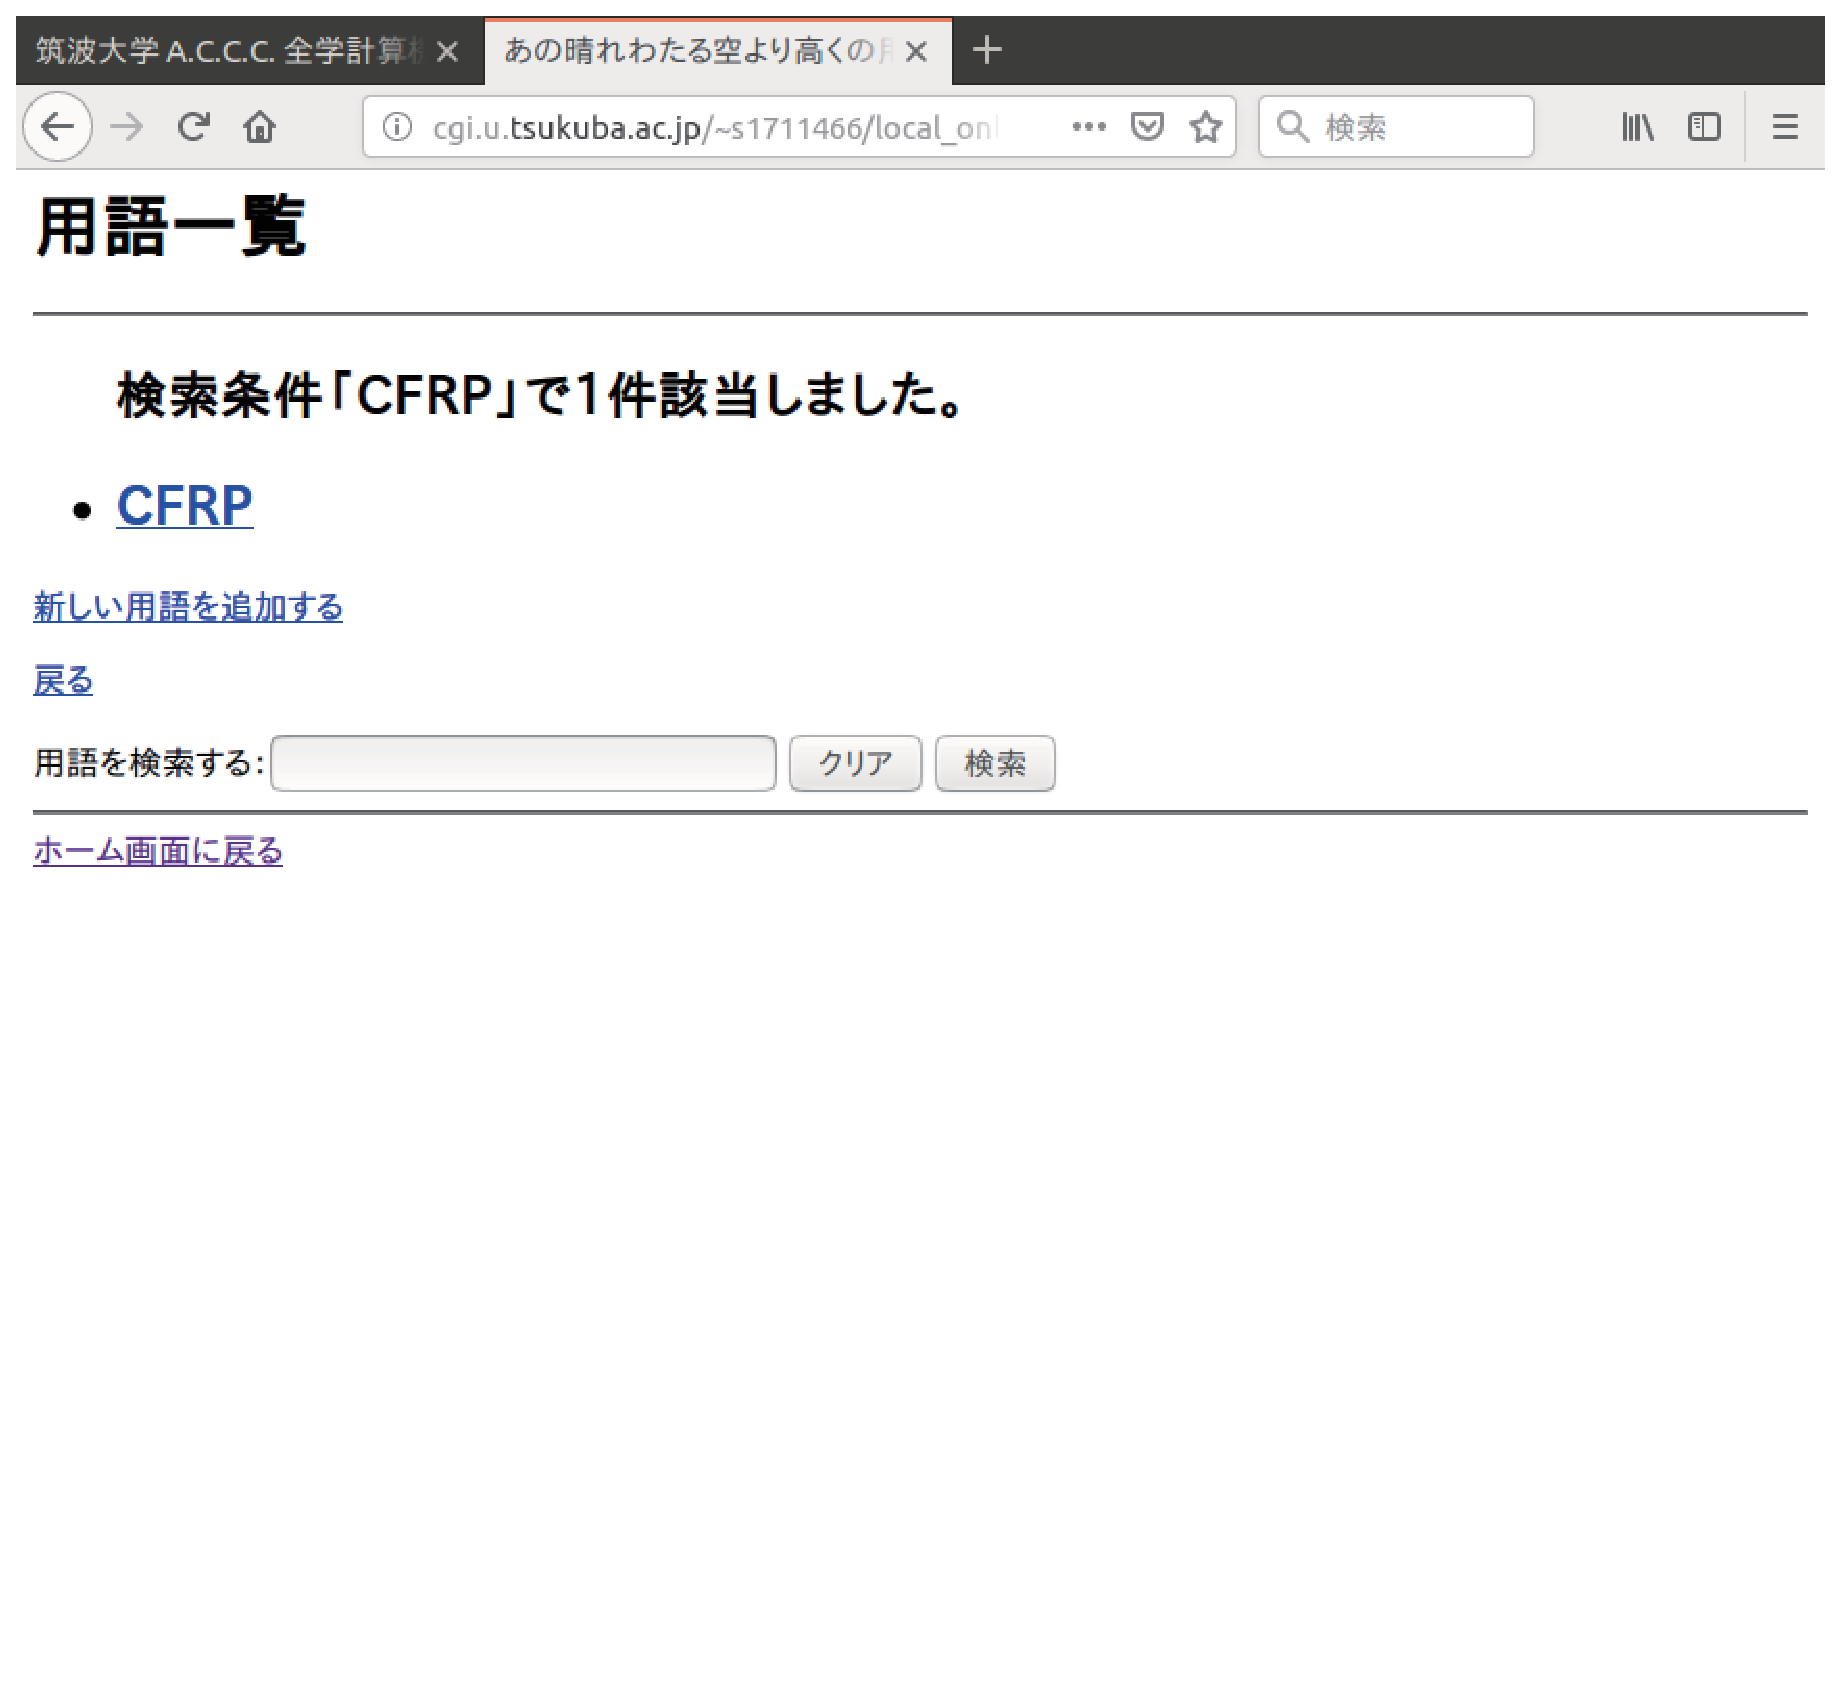
\includegraphics[width=6.7cm]{10-3-42.eps}
          \hspace{1.6cm} [2]検索結果
        \end{center}
      \end{minipage}

    \end{tabular}
    \caption{用語を検索した時の動作画面}
    \label{fig:b}
  \end{center}
\end{figure}

\newpage
\newpage
\newpage
\section{プログラムにアクセスするためのURL}
\verb|http://cgi.u.tsukuba.ac.jp/~s1711466/local_only/wp/universe_editor.rb|

\section{授業の感想}
rubyを使ってwebアプリケーションを作成するという、少し趣向が違う(と個人的に思う)講義だったが、ruby、html、javascriptと浅くではあるが複数の言語を実習形式で学習できたのは貴重な経験になったので良かった。この前に、phpを使ってデータベースを使用する講義もやったが、よりアプリケーションチックな多様な機能があるwebアプリケーションを作成するためのノウハウを段階的に学習し、最後には既存のモノには及ばないまでの比較的さまになるwebアプリケーションを作ることが出来て楽しかった。

\section*{参照文献・参照URL}
\par https://www.sejuku.net/blog/14685
\par https://qiita.com/shizuma/items/4279104026964f1efca6
\par https://allabout.co.jp/gm/gc/23839/
\par https://qiita.com/next1ka2u/items/9736ce2f9c7f3aa69d61
\par http://www.htmq.com/html/input.shtml
\par https://www.tagindex.com/html\_tag/form/textarea.html
\par https://www.dbonline.jp/sqlite/
\par http://www.tohoho-web.com/html/comments.htm


\section*{使用したテキストデータ}
\par https://ja.wikipedia.org/wiki/景の海のアペイリア
\par https://ja.wikipedia.org/wiki/金色ラブリッチェ
\par https://ja.wikipedia.org/wiki/9-nine-ここのつここのかここのいろ
\par https://ja.wikipedia.org/wiki/あの晴れわたる空より高く

\newpage
\section*{ソースコード}
\subsection*{universe\_editor.rb}
\begin{oframed}
 \fontsize{8pt}{8pt}\selectfont
 \begin{verbatim}
#!/usr/bin/env ruby
# encoding: utf-8
require "cgi"
require "sqlite3"
require 'cgi/session'
cgi = CGI.new
session = CGI::Session.new(cgi)
choices = Array.new
world = Array.new
cnt = 0;
url = 'http://cgi.u.tsukuba.ac.jp/~s1711466/local_only/wp/world.rb' # リンク先のURL

print cgi.header("text/html; charset=utf-8")

begin
  db = SQLite3::Database.new("ue.db")
  db.transaction() {
    # 登録されている世界を全て検索し、それのデータをworld.rbに渡すリンクを作成する
    db.execute("SELECT * FROM world;") {|line|
    pass = line[4] # パスワードを格納
    if pass.empty? # パスワードがないなら
      choices.push("<li><form method='get' name='form1' action=#{url}><input type='hidden' name='id' value=#{line[0]}>
<input type='hidden' name='name' value=#{line[1]}><a href='javascript:form1[#{cnt}].submit()'>
#{line[1]}</a>   作成者:#{line[2]}</form></li>")
    else # パスワードがあるなら
      choices.push("<li><form method='get' name='form1' action=#{url} onclick='return gate(\"#{line[4]}\")'>
<input type='hidden' name='id' value=#{line[0]}><input type='hidden' name='name' value=#{line[1]}>
<a href='javascript:form1[#{cnt}].submit()'>#{line[1]}</a>   作成者:#{line[2]}</form></li>")
    end
    cnt += 1
    }
  }
  db.close

  print <<EOB
  <html>
  <head><title>ユニバース・エディタ</title></head>
  <body>
  <script type="text/javascript">
  // パスワード入力ウィンドウ
  function gate(pass){
    var UserInput = prompt("パスワードを入力して下さい:","");
    if(UserInput == pass) {return true;}
    if(UserInput == null) {return false;}
    alert("パスワードが違います");
    return false;
  }
  </script>
  <h1>世界一覧</h1>
  <hr><h2><ul>
  #{choices.join("\n")}
  </ul></h2>
  <a href="http://cgi.u.tsukuba.ac.jp/~s1711466/local_only/wp/world_create.rb">新しい世界をつくる</a>
  </body>
  </html>
EOB
session.close
rescue => ex
  print <<-EOB
  <html><body>
  <p>#{ex.message}</p>
  <p>#{ex.backtrace}</p>
  </body></html>
  EOB
end
 \end{verbatim}
\end{oframed}

\subsection*{world.rb}
\begin{oframed}
 \fontsize{8pt}{8pt}\selectfont
 \begin{verbatim}
#!/usr/bin/env ruby
# encoding: utf-8
require "cgi"
require "sqlite3"
require 'cgi/session'
cgi = CGI.new
session = CGI::Session.new(cgi)
choices = Array.new
world = Array.new
cnt = 0;
urlw = 'http://cgi.u.tsukuba.ac.jp/~s1711466/local_only/wp/words.rb' # 用語一覧のリンク先
urlc = 'http://cgi.u.tsukuba.ac.jp/~s1711466/local_only/wp/chara.rb' # キャラクター一覧のリンク先
name = ""

print cgi.header("text/html; charset=utf-8")

begin
  if cgi["id"].empty?
  else # universe_editor.rbからidとnameが渡されたら、セッション情報を更新する
    name = cgi["name"]
    id = cgi["id"]
    session['name'] = name
    session['id'] = id
  end
  # セッション情報を読み込む
  name = session['name']
  id = session['id']
  print <<EOB
  <html>
  <head><title>#{name}</title></head>
  <body>
  <h1>#{name}</h1>
  <hr><h2><ul>
  <li><form method='get' name='form1' action=#{urlw}>
  <a href='javascript:form1[0].submit()'>用語</a>
  </form></li>
  <li><form method='get' name='form1' action=#{urlc}>
  <a href='javascript:form1[1].submit()'>キャラクター</a>
  </form></li>
  </ul></h2>
  <a href="http://cgi.u.tsukuba.ac.jp/~s1711466/local_only/wp/universe_editor.rb">戻る</a>
  </body></html>
EOB
session.close
rescue => ex
  print <<-EOB
  <html><body>
  <p>#{ex.message}</p>
  <p>#{ex.backtrace}</p>
  </body></html>
  EOB
end
 \end{verbatim}
\end{oframed}

\subsection*{world\_create.rb}
\begin{oframed}
 \fontsize{8pt}{8pt}\selectfont
 \begin{verbatim}
#!/usr/bin/env ruby
# encoding: utf-8
require "cgi"
require 'cgi/session'
cgi = CGI.new
session = CGI::Session.new(cgi)

print cgi.header("text/html; charset=utf-8")

begin
  print <<EOB
  <html><body>
  <h1>新しい世界をつくる</h1>
  <h2>
  <form action="http://cgi.u.tsukuba.ac.jp/~s1711466/local_only/wp/world_create2.rb" method="get">
  <p>名前<input type="text" name="wname"></p>
  <p>作成者<input type="text" name="creator"></p>
  <p>pass<input type="text" name="pass"></p>
  </h2>
  <input type="submit" value="作成">
  <input type="reset" value="クリア">
  <input type="button" value="戻る" onclick="history.back()">
  </form>
  </body></html>
EOB
session.close
rescue => ex
  print <<-EOB
  <html><body>
  <p>#{ex.message}</p>
  <p>#{ex.backtrace}</p>
  </body></html>
  EOB
end
 \end{verbatim}
\end{oframed}

\subsection*{world\_create2.rb}
\begin{oframed}
 \fontsize{8pt}{8pt}\selectfont
 \begin{verbatim}
#!/usr/bin/env ruby
# encoding: utf-8
require "cgi"
require "sqlite3"
require 'cgi/session'
cgi = CGI.new
session = CGI::Session.new(cgi)
cnt = Array.new
w_name = ""
c_name = ""
sqlp = "CREATE TABLE "
sqlw = " (wid INTEGER PRIMARY KEY,creator TEXT NOT NULL,word TEXT NOT NULL,ruby TEXT NOT NULL,
content TEXT NOT NULL,relation TEXT,pass TEXT);" # w○を作成するときのコマンドの一部
sqlc = " (cid INTEGER PRIMARY KEY,creator TEXT NOT NULL,chara TEXT NOT NULL,ruby TEXT NOT NULL,
age INTEGER NOT NULL,sex TEXT NOT NULL,height INTEGER NOT NULL,weight INTEGER NOT NULL,
content TEXT NOT NULL,relation TEXT,pass TEXT);" # c○を作成するときのコマンドの一部

print cgi.header("text/html; charset=utf-8")

begin
  db = SQLite3::Database.new("ue.db")
  db.transaction() {
    # 既に同名の世界があるか判定
    db.execute("SELECT name FROM world;") {|line|
      if line == cgi.params["wname"]
        print <<-EOB
        <html><body>
        <p>#{line[0]}という世界は既に存在します</p>
        <meta http-equiv="refresh" content="1;URL=http://cgi.u.tsukuba.ac.jp/~s1711466/local_only/wp/world_create.rb">
        EOB
        exit
      end
    }
  }
    creator = cgi.params["creator"]
    wname = cgi.params["wname"]
    summary = 'test'
    pass = cgi.params["pass"]
    # 入力漏れがあるか確認
    if creator[0].empty? or wname[0].empty? # パスワードは任意なので見ない
      raise "入力漏れがあります"
    end
    # データベースの処理
    db.transaction() {
      db.execute("INSERT INTO world(name,creator,summary,pass) VALUES(?,?,?,?)", wname,creator,summary,pass) # worldテーブルにデータを追加
      cnt = db.execute("SELECT * FROM world WHERE name = ?;", cgi.params["wname"]) # 追加したデータ(の自動生成されたid)を取得
      w_name = sqlp + "w" + cnt[0][0].to_s + sqlw # w○テーブルを作成するためのコマンドを生成
      c_name = sqlp + "c" + cnt[0][0].to_s + sqlc # c○テーブルを作成するためのコマンドを生成
      db.execute(w_name) # w○テーブルを作成
      db.execute(c_name) # c○テーブルを作成
    }
  db.close

  print <<-EOB
  <html><body>
  <p>新しい世界を作成しました</p>
  <p><a href="http://cgi.u.tsukuba.ac.jp/~s1711466/local_only/wp/universe_editor.rb">戻る</a></p>
  </body></html>
  EOB
  session.close
rescue => ex
  print <<-EOB
  <html><body>
  <pre>#{ex.message}</pre>
  <pre>#{ex.backtrace}</pre>
  EOB
end
 \end{verbatim}
\end{oframed}

\subsection*{words.rb}
\begin{oframed}
 \fontsize{8pt}{8pt}\selectfont
 \begin{verbatim}
#!/usr/bin/env ruby
# encoding: utf-8
require "cgi"
require "sqlite3"
require 'cgi/session'
cgi = CGI.new
session = CGI::Session.new(cgi)
choices = Array.new
world = Array.new
cnt = 0;
url = 'http://cgi.u.tsukuba.ac.jp/~s1711466/local_only/wp/words_page.rb'
urlc = 'http://cgi.u.tsukuba.ac.jp/~s1711466/local_only/wp/words_create.rb'
urlw = 'http://cgi.u.tsukuba.ac.jp/~s1711466/local_only/wp/world.rb'
urlwo = 'http://cgi.u.tsukuba.ac.jp/~s1711466/local_only/wp/words.rb'

print cgi.header("text/html; charset=utf-8")

begin
  # セッション情報を格納
  id = session["id"]
  name = session["name"]
  db = SQLite3::Database.new("ue.db")
  if cgi["search"].empty? # 検索が行われていない場合
    db.transaction() {
      w_name = "w" + id # テーブル名を生成
      sql = "SELECT * FROM " + w_name # テーブルのデータを読み込むためのコマンドを生成
      # 用語ごとに個別ページのリンクを生成
      db.execute(sql) {|line|
      choices.push("<li><form method='post' name='form1' action=#{url}><input type='hidden' name='wid' value=#{line[0]}><a href='javascript:form1[#{cnt}].submit()'>#{line[2]}</a></form></li>")
      cnt += 1
      }
    }
  else # 検索が行われた場合
    db.transaction() {
      search = cgi["search"] #検索条件を格納
      w_name = "w" + id + " WHERE word like ?;" # テーブル名を生成
      sql = "SELECT * FROM " + w_name # テーブルのデータを読み込むためのコマンドを生成
      # 用語ごとに個別ページのリンクを生成
      cnt += 1
      choices.push("<p>検索条件「#{search}」で#{cnt}件該当しました。</p>")
      db.execute(sql,cgi["search"]) {|line|
      choices.push("<li><form method='post' name='form1' action=#{url}><input type='hidden' name='wid' value=#{line[0]}><a href='javascript:form1[#{cnt}].submit()'>#{line[2]}</a></form></li>")
      }
    }
  end
  db.close
  print <<EOB
  <html>
  <head><title>#{name}の用語</title></head>
  <body>
  <h1>用語一覧</h1>
  <hr><h2><ul>
  #{choices.join("\n")}
  </ul></h2>
  <form method='post' name='form2' action=#{urlc}>
  <a href='javascript:form2.submit()'>新しい用語を追加する</a>
  </form>
  <form method='post' name='form3' action=#{urlw}>
  <a href='javascript:form3.submit()'>戻る</a>
  </form>
  <form method='post' action=#{urlwo}>
  <div>用語を検索する:<input type="text" name="search"></dvi>
  <input type="reset" value="クリア">
  <input type="submit" value="検索">
  </form>
  <hr>
  <a href="http://cgi.u.tsukuba.ac.jp/~s1711466/local_only/wp/universe_editor.rb">ホーム画面に戻る</a>
  </body></html>
EOB
session.close
rescue => ex
  print <<-EOB
  <html><body>
  <p>#{ex.message}</p>
  <p>#{ex.backtrace}</p>
  </body></html>
  EOB
end
 \end{verbatim}
\end{oframed}

\subsection*{words\_create.rb}
\begin{oframed}
 \fontsize{8pt}{8pt}\selectfont
 \begin{verbatim}
#!/usr/bin/env ruby
# encoding: utf-8
require "cgi"
require 'cgi/session'
cgi = CGI.new
session = CGI::Session.new(cgi)

print cgi.header("text/html; charset=utf-8")


begin
  # セッション情報を格納
  id = session["id"]
  name = session["name"]
  print <<EOB
  <html><head><title>用語追加</title></head>
  <body>
  <h1>新しい用語を追加する</h>
  <h2>
  <form action="http://cgi.u.tsukuba.ac.jp/~s1711466/local_only/wp/words_create2.rb" method="get">
  <p>作成者<input type="text" name="creator"></p>
  <p>項目名<input type="text" name="word"></p>
  <p>読み<input type="text" name="ruby"></p>
  <p>概要<br><textarea name="content" cols="30" rows="5"></textarea></p>
  <p>pass<input type="text" name="pass"></p>
  </h2>
  <input type="submit" value="作成">
  <input type="reset" value="クリア">
  <input type="button" value="戻る" onclick="history.back()">
  </form>
  </body></html>
EOB
session.close
rescue => ex
  print <<-EOB
  <html><body>
  <p>#{ex.message}</p>
  <p>#{ex.backtrace}</p>
  </body></html>
  EOB
end
 \end{verbatim}
\end{oframed}

\subsection*{words\_create2.rb}
\begin{oframed}
 \fontsize{8pt}{8pt}\selectfont
 \begin{verbatim}
#!/usr/bin/env ruby
# encoding: utf-8
require "cgi"
require "sqlite3"
require 'cgi/session'
cgi = CGI.new
session = CGI::Session.new(cgi)
cnt = Array.new
w_name = "INSERT INTO " # データベースにデータを追加するためのコマンドの一部
s_name = "SELECT word FROM " # データベースを検索するためのコマンドの一部

print cgi.header("text/html; charset=utf-8")


begin
  # セッション情報を格納
  id = session["id"]
  name = session["name"]
  sql = w_name + 'w' + id + ' (creator,word,ruby,content,relation,pass) VALUES(?,?,?,?,?,?)' # データベースにデータを追加するためのコマンドを生成
  db = SQLite3::Database.new("ue.db")
  db.transaction() {
    selectname = s_name + "w" + id + ";" # データベースを検索するためのコマンドを生成
    # 既に同名の用語があるか判定
    db.execute(selectname) {|line|
      if line == cgi.params["word"]
        print <<-EOB
        <html><body>
        <p>#{name}には「#{line[0]}」という用語が既に存在します</p>
        EOB
        exit
      end
    }
  }
   # 正規表現でHTMLタグが使用されているか判定
    creator = cgi.params["creator"]
    if (/<.*>/ !~ creator[0]) == false
      raise "HTMLのタグは使用できません。"
    end
    word = cgi.params["word"]
    if (/<.*>/ !~ word[0]) == false
      raise "HTMLのタグは使用できません。"
    end
    ruby = cgi.params["ruby"]
    if (/<.*>/ !~ ruby[0]) == false
      raise "HTMLのタグは使用できません。"
    end
    content = cgi.params["content"]
    if (/<.*>/ !~ content[0]) == false
      raise "HTMLのタグは使用できません。"
    end
    relation = ''
    pass = cgi.params["pass"]
    if (/<.*>/ !~ pass[0]) == false
      raise "HTMLのタグは使用できません。"
    end
    db.transaction() {
      db.execute(sql, creator,word,ruby,content,relation,pass) # w○テーブルにデータを追加
    }
  db.close

  print <<-EOB
  <html><body>
  <p>新しい用語を追加しました</p>
  <form method='get' name='form1' action="http://cgi.u.tsukuba.ac.jp/~s1711466/local_only/wp/words.rb">
  <a href='javascript:form1.submit()'>戻る</a>
  </body></html>
  EOB
  session.close
rescue => ex
  print <<-EOB
  <html><body>
  <pre>#{ex.message}</pre>
  <pre>#{ex.backtrace}</pre>
  EOB
end
 \end{verbatim}
\end{oframed}

\subsection*{words\_page.rb}
\begin{oframed}
 \fontsize{8pt}{8pt}\selectfont
 \begin{verbatim}
#!/usr/bin/env ruby
# encoding: utf-8
require "cgi"
require "sqlite3"
require 'cgi/session'
cgi = CGI.new
session = CGI::Session.new(cgi)
choices = Array.new
word = Array.new
cnt = 0;
sql = ""
urlw = 'http://cgi.u.tsukuba.ac.jp/~s1711466/local_only/wp/words.rb' # 用語一覧ページへのリンク
urle = 'http://cgi.u.tsukuba.ac.jp/~s1711466/local_only/wp/words_edit.rb' # 用語編集ページへのリンク

print cgi.header("text/html; charset=utf-8")

begin
  wid = cgi["wid"]
  # セッション情報を格納
  id = session["id"]
  name = session["name"]
  db = SQLite3::Database.new("ue.db")
  db.transaction() {
    w_name = "w" + id # テーブル名を生成
    sql = "SELECT * FROM " + w_name + " WHERE wid = ?" # データベースを検索するためのコマンドを生成
    word = db.execute(sql, wid) # 検索したデータベースの情報を格納
  }
  db.close

  print <<EOB
  <html>
  <head><title>#{name}の用語:#{word[0][2]}</title></head>
  <body>
  <h1>#{word[0][2]} (#{word[0][3]})</h1>
  <h3><p style="text-align: right">作成者 #{word[0][1]}</p></h3>
  <hr><h3>
  <p>#{word[0][4].gsub(/\n/, '</br>')}</p><!-- 正規表現によって改行文字「\n」を「</br>」に置換する -->
  </h3>
  <form method='get' name='form3' action=#{urle}>
  <input type='hidden' name='wid' value=#{word[0][0]}>
  <a href='javascript:form3.submit()'>内容を編集する</a>
  </form>
  <form method='get' name='form4' action=#{urlw}>
  <a href='javascript:form4.submit()'>戻る</a>
  </form>
  </body></html>
EOB
session.close
rescue => ex
  print <<-EOB
  <html><body>
  <p>#{ex.message}</p>
  <p>#{ex.backtrace}</p>
  </body></html>
  EOB
end
 \end{verbatim}
\end{oframed}

\subsection*{words\_edit.rb}
\begin{oframed}
 \fontsize{8pt}{8pt}\selectfont
 \begin{verbatim}
#!/usr/bin/env ruby
# encoding: utf-8
require "cgi"
require "sqlite3"
require 'cgi/session'
cgi = CGI.new
session = CGI::Session.new(cgi)
pass = Array.new

print cgi.header("text/html; charset=utf-8")

begin
  # セッション情報を格納
  id = session["id"]
  name = session["name"]
  wid = cgi["wid"]
  passsen = "SELECT pass FROM " + "w" + id + " WHERE wid = ?;" # その用語に設けられたパスワードを検索するためのコマンドを生成
  db = SQLite3::Database.new("ue.db")
  db.transaction() {
     # パスワードを検索し、格納
    db.execute(passsen,wid) {|line|
      pass = line
    }
  }
  db.close
  print <<EOB
  <html>
  <head><title>用語編集</title></head>
  <body>
  <script type="text/javascript">
  function gate(pass){
    var str = pass; // 引数にして取得したpassを格納
    // strの長さが0でない(=パスワードがある)ならパスワード入力を要求する
    if(str.length != 0) {
      var UserInput = prompt("パスワードを入力して下さい:","");
      if(UserInput == pass) {return true;}
      if(UserInput == null) {return false;}
      alert("パスワードが違います");
      return false;
    }
  }
  </script>
  <h1>用語を編集する</h1>
  <h2>
  <form action="http://cgi.u.tsukuba.ac.jp/~s1711466/local_only/wp/words_edit2.rb" method="get" 
onSubmit="return gate('#{pass[0]}')">
  <p>作成者<input type="text" name="creator"></p>
  <p>項目名<input type="text" name="word"></p>
  <p>読み<input type="text" name="ruby"></p>
  <p>概要<br><textarea name="content" cols="30" rows="5"></textarea></p>
  <p>pass<input type="text" name="pass"></p>
  </h2>
  <input type='hidden' name='wid' value=#{wid}>
  <input type="submit" value="変更">
  <input type="reset" value="クリア">
  <input type="submit" name='delete' value="削除">
  <input type="button" value="戻る" onclick="history.back()">
  </form>
  </body></html>
EOB
session.close
rescue => ex
  print <<-EOB
  <html><body>
  <p>#{ex.message}</p>
  <p>#{ex.backtrace}</p>
  </body></html>
  EOB
end
 \end{verbatim}
\end{oframed}

\subsection*{words\_edit2.rb}
\begin{oframed}
 \fontsize{8pt}{8pt}\selectfont
 \begin{verbatim}
#!/usr/bin/env ruby
# encoding: utf-8
require "cgi"
require "sqlite3"
require 'cgi/session'
cgi = CGI.new
session = CGI::Session.new(cgi)
cnt = Array.new
w_name = "update " # データベースのデータを更新するコマンドの一部
d_name = "DELETE FROM " # データベースのデータを削除するコマンドの一部

print cgi.header("text/html; charset=utf-8")

begin
  # セッション情報を格納
  id = session["id"]
  name = session["name"]
  wid = cgi["wid"]
  sql = w_name + 'w' + id + ' set' # データベースのデータを更新するコマンドを生成

  db = SQLite3::Database.new("ue.db")
   # words_editで削除ボタンが押されていたら用語を削除する
  dflag = cgi["delete"]
  if cgi["delete"].empty?
  else
    d = d_name + "w" + id + " WHERE wid = ?;" # データベースのデータを削除するコマンドを生成
    db.transaction() {db.execute(d, wid)} # 用語のデータを削除
    print <<-EOB
    <html><body>
    <p>用語を削除しました</p>
    <form method='get' name='form1' action="http://cgi.u.tsukuba.ac.jp/~s1711466/local_only/wp/words.rb">
    <a href='javascript:form1.submit()'>戻る</a>
    </body></html>
    EOB
    db.close
    exit
  end
   # 正規表現でHTMLのタグが使用されているか判定
    creator = cgi.params["creator"]
    if (/<.*>/ !~ creator[0]) == false
      raise "HTMLのタグは使用できません。"
    end
    word = cgi.params["word"]
    if (/<.*>/ !~ word[0]) == false
      raise "HTMLのタグは使用できません。"
    end
    ruby = cgi.params["ruby"]
    if (/<.*>/ !~ ruby[0]) == false
      raise "HTMLのタグは使用できません。"
    end
    content = cgi.params["content"]
    if (/<.*>/ !~ content[0]) == false
      raise "HTMLのタグは使用できません。"
    end
    relation = ''
    pass = cgi.params["pass"]
    if (/<.*>/ !~ pass[0]) == false
      raise "HTMLのタグは使用できません。"
    end
  # words_editで入力があった項目を更新
  if cgi["creator"].empty?
  else
    n = sql + ' creator = ? where wid = ?;'
    db.transaction() {db.execute(n, cgi["creator"], wid)}
  end
  if cgi["ruby"].empty?
  else
    n = sql + ' ruby = ? where wid = ?;'
    db.transaction() {db.execute(n, cgi["ruby"], wid)}
  end
  if cgi["content"].empty?
  else
    n = sql + ' content = ? where wid = ?;'
    db.transaction() {db.execute(n, cgi["content"], wid)}
  end
  if cgi["pass"].empty?
  else
    n = sql + ' pass = ? where wid = ?;'
    db.transaction() {db.execute(n, cgi["pass"], wid)}
  end
  if cgi["word"].empty?
  else
    n = sql + ' word = ? where wid = ?;'
    db.transaction() {db.execute(n, cgi["word"], wid)}
  end
  db.close

  print <<-EOB
  <html><body>
  <p>用語の情報を編集しました</p>
  <form method='get' name='form1' action="http://cgi.u.tsukuba.ac.jp/~s1711466/local_only/wp/words_page.rb">
  <input type='hidden' name='wid' value=#{wid}>
  <a href='javascript:form1.submit()'>戻る</a>
  </body></html>
  EOB
  session.close
rescue => ex
  print <<-EOB
  <html><body>
  <pre>#{ex.message}</pre>
  <pre>#{ex.backtrace}</pre>
  EOB
end
 \end{verbatim}
\end{oframed}

\subsection*{chara.rb}
\begin{oframed}
 \fontsize{8pt}{8pt}\selectfont
 \begin{verbatim}
#!/usr/bin/env ruby
# encoding: utf-8
require "cgi"
require "sqlite3"
require 'cgi/session'
cgi = CGI.new
session = CGI::Session.new(cgi)
choices = Array.new
world = Array.new
cnt = 0;
url = 'http://cgi.u.tsukuba.ac.jp/~s1711466/local_only/wp/chara_page.rb' # 個別(詳細)ページへのリンク
urlc = 'http://cgi.u.tsukuba.ac.jp/~s1711466/local_only/wp/chara_create.rb' # キャラクター追加ページへのリンク
urlw = 'http://cgi.u.tsukuba.ac.jp/~s1711466/local_only/wp/world.rb' # 前ページへのリンク

print cgi.header("text/html; charset=utf-8")

begin
  # セッション情報を格納
  id = session["id"]
  name = session["name"]
  db = SQLite3::Database.new("ue.db")
  db.transaction() {
    c_name = "c" + id # テーブル名を生成
    sql = "SELECT * FROM " + c_name # テーブルのデータを読み込むためのコマンドを生成
    # 用語ごとに個別ページのリンクを生成
    db.execute(sql) {|line|
    choices.push("<li><form method='get' name='form1' action=#{url}><input type='hidden' name='cid' value=#{line[0]}>
<a href='javascript:form1[#{cnt}].submit()'>#{line[2]}</a></form></li>")
    cnt += 1
    }
  }
  db.close

  print <<EOB
  <html>
  <head><title>#{name}のキャラクター</title></head>
  <body>
  <h1>キャラクター一覧</h>
  <hr><h2><ul>
  #{choices.join("\n")}
  </ul></h2>
  <form method='get' name='form2' action=#{urlc}>
  <a href='javascript:form2.submit()'>新しいキャラクターを追加する</a>
  </form>
  <form method='get' name='form3' action=#{urlw}>
  <a href='javascript:form3.submit()'>戻る</a>
  </form>
  <hr>
  <a href="http://cgi.u.tsukuba.ac.jp/~s1711466/local_only/wp/universe_editor.rb">ホーム画面に戻る</a>
  </body></html>
EOB
session.close
rescue => ex
  print <<-EOB
  <html><body>
  <p>#{ex.message}</p>
  <p>#{ex.backtrace}</p>
  </body></html>
  EOB
end
 \end{verbatim}
\end{oframed}

\subsection*{chara\_create.rb}
\begin{oframed}
 \fontsize{8pt}{8pt}\selectfont
 \begin{verbatim}
#!/usr/bin/env ruby
# encoding: utf-8
require "cgi"
require 'cgi/session'
cgi = CGI.new
session = CGI::Session.new(cgi)

print cgi.header("text/html; charset=utf-8")


begin
  # セッション情報を格納
  id = session["id"]
  name = session["name"]
  print <<EOB
  <html><head><title>キャラクター追加</title></head>
  <body>
  <h1>新しいキャラクターを追加する</h1>
  <h2>
  <form action="http://cgi.u.tsukuba.ac.jp/~s1711466/local_only/wp/chara_create2.rb" method="get">
  <p>作成者<input type="text" name="creator"></p>
  <p>キャラクター名<input type="text" name="chara"></p>
  <p>読み<input type="text" name="ruby"></p>
  <p>年齢<input type="text" name="age">歳</p>
  <p>性別<input type="text" name="sex"></p>
  <p>身長<input type="text" name="height">cm</p>
  <p>体重<input type="text" name="weight">kg</p>
  <p>概要<br><textarea name="content" cols="30" rows="5"></textarea></p>
  <p>pass<input type="text" name="pass"></p>
  </h2>
  <input type="submit" value="作成">
  <input type="reset" value="クリア">
  <input type="button" value="戻る" onclick="history.back()">
  </form>
  </body></html>
EOB
session.close
rescue => ex
  print <<-EOB
  <html><body>
  <p>#{ex.message}</p>
  <p>#{ex.backtrace}</p>
  </body></html>
  EOB
end
 \end{verbatim}
\end{oframed}

\subsection*{chara\_create2.rb}
\begin{oframed}
 \fontsize{8pt}{8pt}\selectfont
 \begin{verbatim}
#!/usr/bin/env ruby
# encoding: utf-8
require "cgi"
require "sqlite3"
require 'cgi/session'
cgi = CGI.new
session = CGI::Session.new(cgi)
cnt = Array.new
c_name = "INSERT INTO " # データベースにデータを追加するためのコマンドの一部
s_name = "SELECT chara FROM " # データベースを検索するためのコマンドの一部

print cgi.header("text/html; charset=utf-8")


begin
  # セッション情報を格納
  id = session["id"]
  name = session["name"]
  sql = c_name + 'c' + id + ' (creator,chara,ruby,age,sex,height,weight,content,relation,pass) VALUES(?,?,?,?,?,?,?,?,?,?)' # データベースにデータを追加するためのコマンドを生成
  db = SQLite3::Database.new("ue.db")
  db.transaction() {
    selectname = s_name + "c" + id + ";" # データベースを検索するためのコマンドを生成
    # 既に同名のキャラクターがあるか判定
    db.execute(selectname) {|line|
      if line == cgi.params["chara"]
        print <<-EOB
        <html><body>
        <p>#{name}には「#{line[0]}」というキャラクターが既に存在します</p>
        EOB
        exit
      end
    }
  }
   # 正規表現でHTMLタグが使用されているか判定
    creator = cgi.params["creator"]
    if (/<.*>/ !~ creator[0]) == false
      raise "HTMLのタグは使用できません。"
    end
    chara = cgi.params["chara"]
    if (/<.*>/ !~ chara[0]) == false
      raise "HTMLのタグは使用できません。"
    end
    ruby = cgi.params["ruby"]
    if (/<.*>/ !~ ruby[0]) == false
      raise "HTMLのタグは使用できません。"
    end
    age = cgi.params["age"]
    if (/<.*>/ !~ age.to_s) == false
      raise "HTMLのタグは使用できません。"
    end
    sex = cgi.params["sex"]
    if (/<.*>/ !~ sex[0]) == false
      raise "HTMLのタグは使用できません。"
    end
    height = cgi.params["height"]
    if (/<.*>/ !~ height.to_s) == false
      raise "HTMLのタグは使用できません。"
    end
    weight = cgi.params["weight"]
    if (/<.*>/ !~ weight.to_s) == false
      raise "HTMLのタグは使用できません。"
    end
    content = cgi.params["content"]
    if (/<.*>/ !~ content[0]) == false
      raise "HTMLのタグは使用できません。"
    end
    relation = ''
    pass = cgi.params["pass"]
    if (/<.*>/ !~ pass[0]) == false
      raise "HTMLのタグは使用できません。"
    end
    db.transaction() {
      db.execute(sql, creator,chara,ruby,age,sex,height,weight,content,relation,pass) # c○テーブルにデータを追加
    }
  db.close

  print <<-EOB
  <html><body>
  <p>新しいキャラクターを追加しました</p>
  <form method='get' name='form1' action="http://cgi.u.tsukuba.ac.jp/~s1711466/local_only/wp/chara.rb">
  <a href='javascript:form1.submit()'>戻る</a>
  </body></html>
  EOB
  session.close
rescue => ex
  print <<-EOB
  <html><body>
  <pre>#{ex.message}</pre>
  <pre>#{ex.backtrace}</pre>
  EOB
end
 \end{verbatim}
\end{oframed}

\subsection*{create\_page.rb}
\begin{oframed}
 \fontsize{8pt}{8pt}\selectfont
 \begin{verbatim}
#!/usr/bin/env ruby
# encoding: utf-8
require "cgi"
require "sqlite3"
require 'cgi/session'
cgi = CGI.new
session = CGI::Session.new(cgi)
choices = Array.new
chara = Array.new
cnt = 0;
sql = ""
urlw = 'http://cgi.u.tsukuba.ac.jp/~s1711466/local_only/wp/chara.rb' # キャラクター一覧ページへのリンク
urle = 'http://cgi.u.tsukuba.ac.jp/~s1711466/local_only/wp/chara_edit.rb' # キャラクター編集ページへのリンク
ex = "<h1><p>akak</p></h1>"

print cgi.header("text/html; charset=utf-8")

begin
  cid = cgi["cid"]
  # セッション情報を格納
  id = session["id"]
  name = session["name"]
  db = SQLite3::Database.new("ue.db")
  db.transaction() {
    w_name = "c" + id # テーブル名を生成
    sql = "SELECT * FROM " + w_name + " WHERE cid = ?" # データベースを検索するためのコマンドを生成
    chara = db.execute(sql, cid) # 検索したデータベースの情報を格納
  }
  db.close

  print <<EOB
  <html>
  <head><title>#{name}のキャラクター:#{chara[0][1]}</title></head>
  <body>
  <h1>#{chara[0][2]} (#{chara[0][3]})</h1>
  <h3><p style="text-align: right">作成者 #{chara[0][1]}</p></h3>
  <hr><h4>
  <p>年齢:#{chara[0][4]}歳</p>
  <p>性別:#{chara[0][5]}</p>
  <p>身長:#{chara[0][6]}cm</p>
  <p>体重:#{chara[0][7]}kg</p>
  </h4>
  <h3>
  <br></br>
  <p>#{chara[0][8].gsub(/\n/, '</br>')}</p><!-- 正規表現によって改行文字「\n」を「</br>」に置換する -->
  </h3>
  <form method='get' name='form3' action=#{urle}>
  <input type='hidden' name='cid' value=#{chara[0][0]}>
  <a href='javascript:form3.submit()'>内容を編集する</a>
  </form>
  <form method='get' name='form4' action=#{urlw}>
  <a href='javascript:form4.submit()'>戻る</a>
  </form>
  </body></html>
EOB
session.close
rescue => ex
  print <<-EOB
  <html><body>
  <p>#{ex.message}</p>
  <p>#{ex.backtrace}</p>
  </body></html>
  EOB
end
 \end{verbatim}
\end{oframed}

\subsection*{create\_edit.rb}
\begin{oframed}
 \fontsize{8pt}{8pt}\selectfont
 \begin{verbatim}
#!/usr/bin/env ruby
# encoding: utf-8
require "cgi"
require "sqlite3"
require 'cgi/session'
cgi = CGI.new
session = CGI::Session.new(cgi)
pass = Array.new

print cgi.header("text/html; charset=utf-8")

begin
  # セッション情報を格納
  id = session["id"]
  name = session["name"]
  cid = cgi["cid"]
  passsen = "SELECT pass FROM " + "c" + id + " WHERE cid = ?;" # その用語に設けられたパスワードを検索するためのコマンドを生成
  db = SQLite3::Database.new("ue.db")
  db.transaction() {
     # パスワードを検索し、格納
    db.execute(passsen,cid) {|line|
      pass = line
    }
  }
  db.close
  print <<EOB
  <html>
  <head><title>キャラクター編集</title></head>
  <body>
  <script type="text/javascript">
  function gate(pass){
    var str = pass; // 引数にして取得したpassを格納
    // strの長さが0でない(=パスワードがある)ならパスワード入力を要求する
    if(str.length != 0) {
      var UserInput = prompt("パスワードを入力して下さい:","");
      if(UserInput == pass) {return true;}
      if(UserInput == null) {return false;}
      alert("パスワードが違います");
      return false;
    }
  }
  </script>
  <h1>キャラクターを編集する</h1>
  <h2>
  <form action="http://cgi.u.tsukuba.ac.jp/~s1711466/local_only/wp/chara_edit2.rb" method="get" 
onSubmit="return gate('#{pass[0]}')">
  <p>作成者<input type="text" name="creator"></p>
  <p>キャラクター名<input type="text" name="chara"></p>
  <p>読み<input type="text" name="ruby"></p>
  <p>年齢<input type="text" name="age"> 歳</p>
  <p>性別<input type="text" name="sex"></p>
  <p>身長<input type="text" name="height"> cm</p>
  <p>体重<input type="text" name="weight"> kg</p>
  <p>概要<br><textarea name="content" cols="30" rows="5"></textarea></p>
  <p>pass<input type="text" name="pass"></p>
  </h2>
  <input type='hidden' name='cid' value=#{cid}>
  <input type="submit" value="変更">
  <input type="reset" value="クリア">
  <input type="submit" name='delete' value="削除">
  <input type="button" value="戻る" onclick="history.back()">
  </form>
  </body></html>
EOB
session.close
rescue => ex
  print <<-EOB
  <html><body>
  <p>#{ex.message}</p>
  <p>#{ex.backtrace}</p>
  </body></html>
  EOB
end
 \end{verbatim}
\end{oframed}

\subsection*{create\_edit2.rb}
\begin{oframed}
 \fontsize{8pt}{8pt}\selectfont
 \begin{verbatim}
#!/usr/bin/env ruby
# encoding: utf-8
require "cgi"
require "sqlite3"
require 'cgi/session'
cgi = CGI.new
session = CGI::Session.new(cgi)
cnt = Array.new
w_name = "update " # データベースのデータを更新するコマンドの一部
d_name = "DELETE FROM " # データベースのデータを削除するコマンドの一部

print cgi.header("text/html; charset=utf-8")

begin
  # セッション情報を格納
  id = session["id"]
  name = session["name"]
  cid = cgi["cid"]
  sql = w_name + 'c' + id + ' set' # データベースのデータを更新するコマンドを生成

  db = SQLite3::Database.new("ue.db")
   # chara_editで削除ボタンが押されていたら用語を削除する
  dflag = cgi["delete"]
  if cgi["delete"].empty?
  else
    d = d_name + "c" + id + " WHERE cid = ?;" # データベースのデータを削除するコマンドを生成
    db.transaction() {db.execute(d, cid)} # キャラクターのデータを削除
    print <<-EOB
    <html><body>
    <p>キャラクターを削除しました</p>
    <form method='get' name='form1' action="http://cgi.u.tsukuba.ac.jp/~s1711466/local_only/wp/chara.rb">
    <a href='javascript:form1.submit()'>戻る</a>
    </body></html>
    EOB
    db.close
    exit
  end
   # 正規表現でHTMLのタグが使用されているか判定
    creator = cgi.params["creator"]
    if (/<.*>/ !~ creator[0]) == false
      raise "HTMLのタグは使用できません。"
    end
    chara = cgi.params["chara"]
    if (/<.*>/ !~ chara[0]) == false
      raise "HTMLのタグは使用できません。"
    end
    ruby = cgi.params["ruby"]
    if (/<.*>/ !~ ruby[0]) == false
      raise "HTMLのタグは使用できません。"
    end
    age = cgi.params["age"]
    if (/<.*>/ !~ age.to_s) == false
      raise "HTMLのタグは使用できません。"
    end
    sex = cgi.params["sex"]
    if (/<.*>/ !~ sex[0]) == false
      raise "HTMLのタグは使用できません。"
    end
    height = cgi.params["height"]
    if (/<.*>/ !~ height.to_s) == false
      raise "HTMLのタグは使用できません。"
    end
    weight = cgi.params["weight"]
    if (/<.*>/ !~ weight.to_s) == false
      raise "HTMLのタグは使用できません。"
    end
    content = cgi.params["content"]
    if (/<.*>/ !~ content[0]) == false
      raise "HTMLのタグは使用できません。"
    end
    relation = ''
    pass = cgi.params["pass"]
    if (/<.*>/ !~ pass[0]) == false
      raise "HTMLのタグは使用できません。"
    end
  # chara_editで入力があった項目を更新
  if cgi["creator"].empty?
  else
    n = sql + ' creator = ? where cid = ?;'
    db.transaction() {db.execute(n, cgi["creator"], cid)}
  end
  if cgi["ruby"].empty?
  else
    n = sql + ' ruby = ? where cid = ?;'
    db.transaction() {db.execute(n, cgi["ruby"], cid)}
  end
  if cgi["age"].empty?
  else
    n = sql + ' age = ? where cid = ?;'
    db.transaction() {db.execute(n, cgi["age"], cid)}
  end
  if cgi["sex"].empty?
  else
    n = sql + ' sex = ? where cid = ?;'
    db.transaction() {db.execute(n, cgi["sex"], cid)}
  end
  if cgi["height"].empty?
  else
    n = sql + ' height = ? where cid = ?;'
    db.transaction() {db.execute(n, cgi["height"], cid)}
  end
  if cgi["weight"].empty?
  else
    n = sql + ' weight = ? where cid = ?;'
    db.transaction() {db.execute(n, cgi["weight"], cid)}
  end
  if cgi["content"].empty?
  else
    n = sql + ' content = ? where cid = ?;'
    db.transaction() {db.execute(n, cgi["content"], cid)}
  end
  if cgi["pass"].empty?
  else
    n = sql + ' pass = ? where cid = ?;'
    db.transaction() {db.execute(n, cgi["pass"], cid)}
  end
  if cgi["chara"].empty?
  else
    n = sql + ' chara = ? where cid = ?;'
    db.transaction() {db.execute(n, cgi["chara"], cid)}
  end
  db.close

  print <<-EOB
  <html><body>
  <p>キャラクターの情報を編集しました</p>
  <form method='get' name='form1' action="http://cgi.u.tsukuba.ac.jp/~s1711466/local_only/wp/chara_page.rb">
  <input type='hidden' name='cid' value=#{cid}>
  <a href='javascript:form1.submit()'>戻る</a>
  </body></html>
  EOB
  session.close
rescue => ex
  print <<-EOB
  <html><body>
  <pre>#{ex.message}</pre>
  <pre>#{ex.backtrace}</pre>
  EOB
end
 \end{verbatim}
\end{oframed}

\end{ttfamily}
\end{document}
